\chapter{3 \glsentrytext{dof} localization system results} \label{app:appendix-a}



\section*{}

The next sections present in detail the results achieved with the localization system configured to 3 \gls{dof}.

Each test starts by presenting an interactive sequence of images in order to give an overview of the sensor data retrieved along the movement path of the robot (a regular grid with 1 meter spacing and a inner grid with 5 cm were applied on top of the figures). To allow a more broad analysis of the point cloud registration quality achieved with the proposed localization system, it is also provided figures with all the lasers assembled using the estimated robot poses. For a more visual inspection, the synchronized poses from the localization system (blue arrows), ground truth (green arrows), odometry (red arrows) and \gls{amcl} (brown arrows) are also presented. To have a much more detailed description of the robot movement path, several more graphs are shown with information about the evolution of the x and y position, along with the distance that the robot traveled between pose estimations and the associated linear / angular velocities / accelerations. Later on, the translation and rotation errors and their respective probability distributions are shown. To give an overview of the impact of the localization system over the odometry movement estimations, the translation and rotation corrections are also given. In the end, it is presented some graphs with information about the point clouds size in each of the main processing stages of the localization system pipeline, along with the number of registered points, inliers analysis (percentage, \gls{rmse} and angular distribution) and finally some more graphs showing how much time the localization system required for each pose estimation.

Only the most representative tests are shown in the next sections. In \footnote{\url{https://github.com/carlosmccosta/dynamic_robot_localization_tests}} is available the full test results along with videos and the configurations used.


\clearpage
\section{Jarvis robot tests}

The next subsections show some of the most relevant results retrieved with the Jarvis robot in the RoboCup field.

\subsection{Rounded path using the Jarvis robot at 5 cm/s}\label{subsec:appendix-a_jarvis-robot-tests_rounded-path-using-the-jarvis-robot-at-5-cm-s}

The figures in this section show the detailed results of the the test performed with the Jarvis robot with a 10 mm resolution map in the RoboCup field following a rounded path and moving at 5 cm/s.


%Animated paths
\begin{figure}[H]
	\centering
	\animategraphics[width=0.63\textwidth,loop,autoplay,controls]{1}{appendices/tests-3dof/jarvis-robot/\currfilebase/images-ground-truth/image}{1}{10}
	\caption{Laser scans projected on top of the map using the ground truth poses}
\end{figure}

\begin{figure}[H]
	\centering
	\animategraphics[width=0.63\textwidth,loop,autoplay,controls]{1}{appendices/tests-3dof/jarvis-robot/\currfilebase/images-drl/image}{1}{10}
	\caption{Laser scans projected on top of the map using the localization system poses}
\end{figure}

\begin{figure}[H]
	\centering
	\animategraphics[width=0.63\textwidth,loop,autoplay,controls]{1}{appendices/tests-3dof/jarvis-robot/\currfilebase/images-amcl/image}{1}{10}
	\caption{Laser scans projected on top of the map using the \glsentrytext{amcl} poses}
\end{figure}


%Laser assembly
\begin{figure}[H]
	\centering
	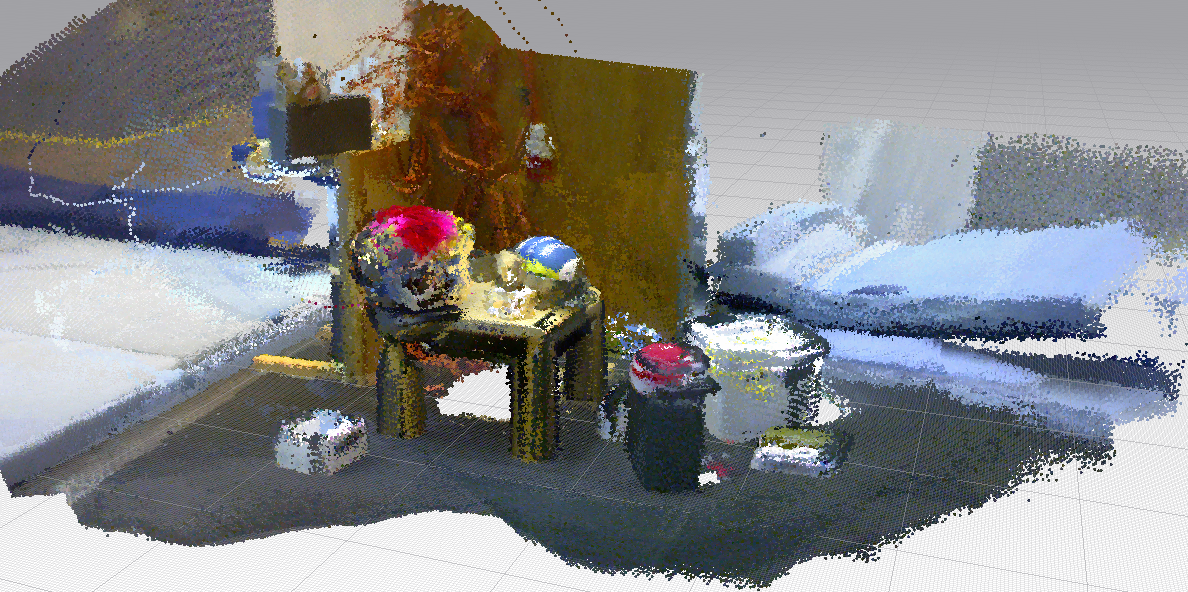
\includegraphics[width=0.993\textwidth]{appendices/tests-3dof/jarvis-robot/\currfilebase/ground-truth-cumulative}
	\caption{Laser scans assembled on top of the map using the ground truth poses}
\end{figure}

\begin{figure}[H]
	\centering
	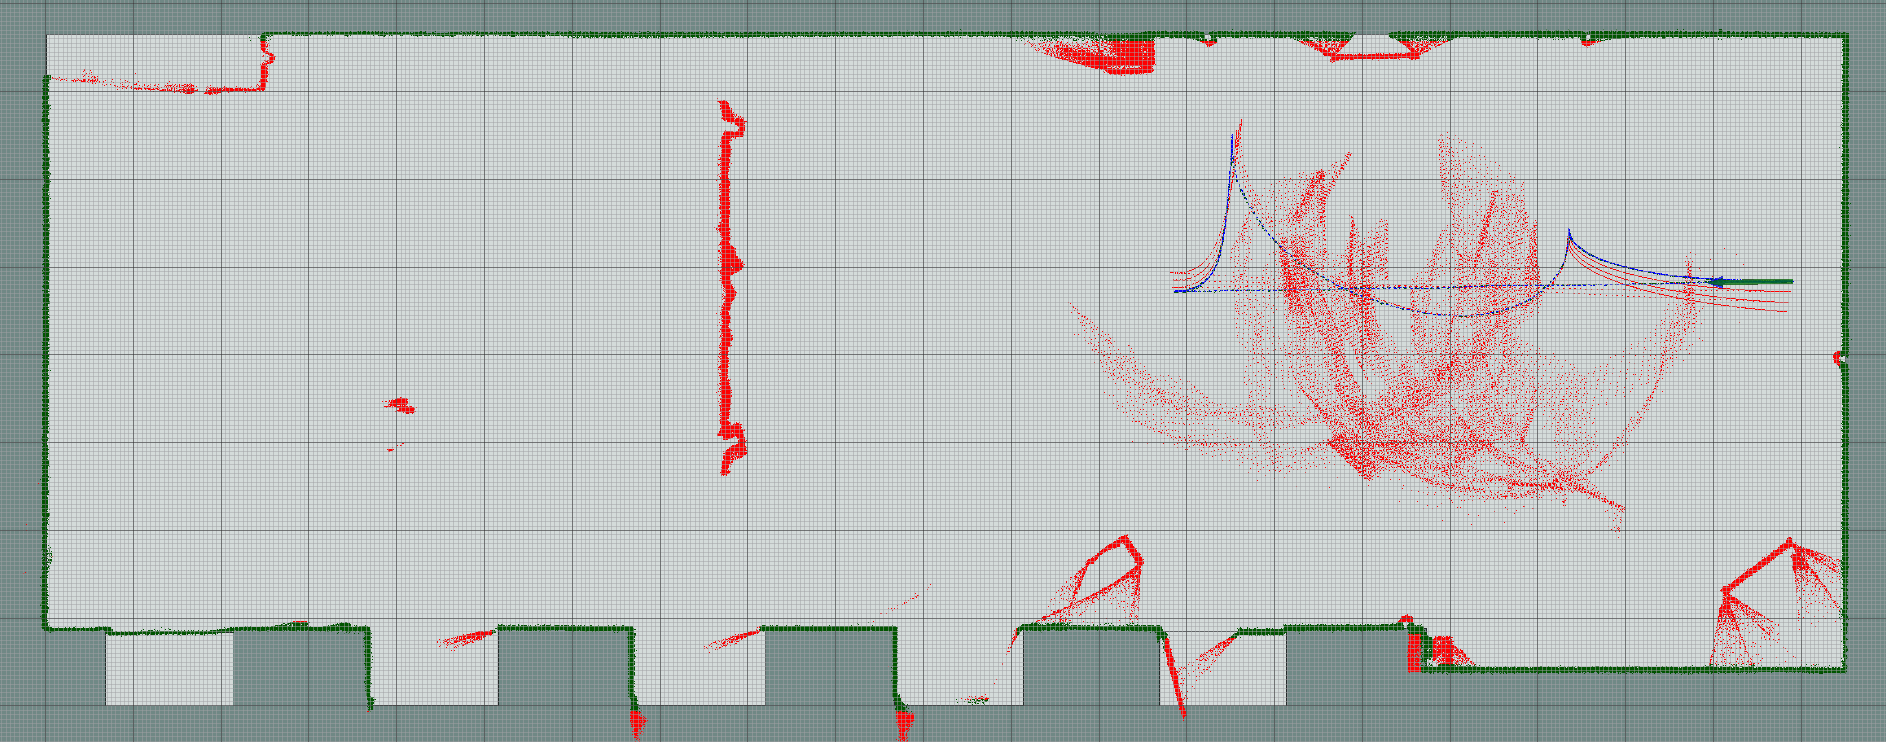
\includegraphics[width=0.993\textwidth]{appendices/tests-3dof/jarvis-robot/\currfilebase/drl-cumulative}
	\caption{Laser scans assembled on top of the map using the localization system poses}
\end{figure}

\begin{figure}[H]
	\centering
	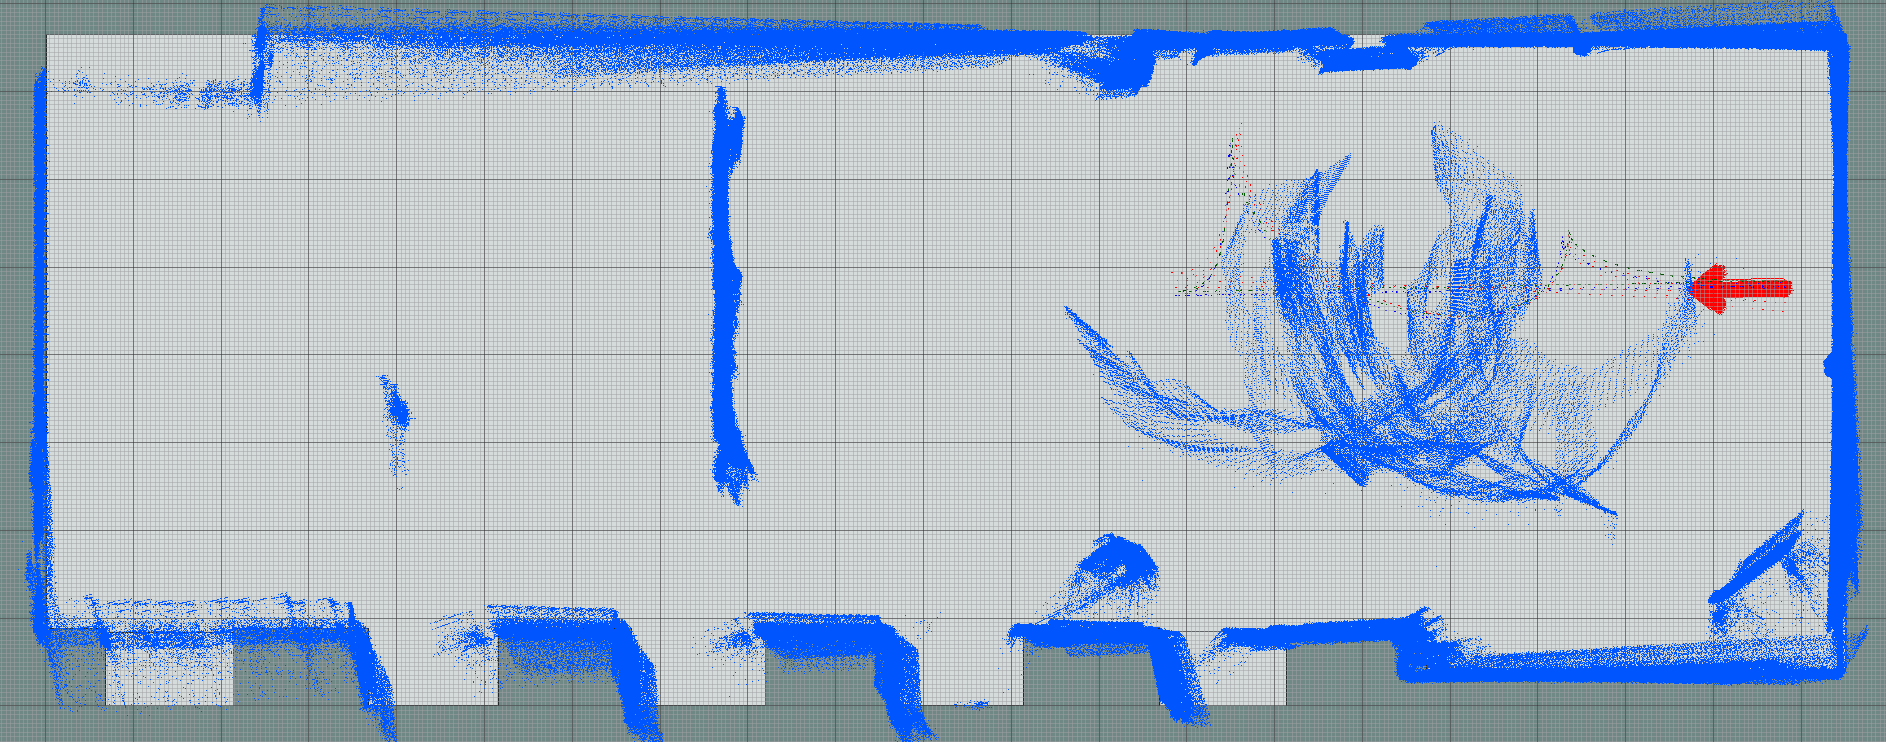
\includegraphics[width=0.993\textwidth]{appendices/tests-3dof/jarvis-robot/\currfilebase/amcl-cumulative}
	\caption{Laser scans assembled on top of the map using the \glsentrytext{amcl} poses}
\end{figure}


%Paths
\begin{figure}[H]
	\centering
	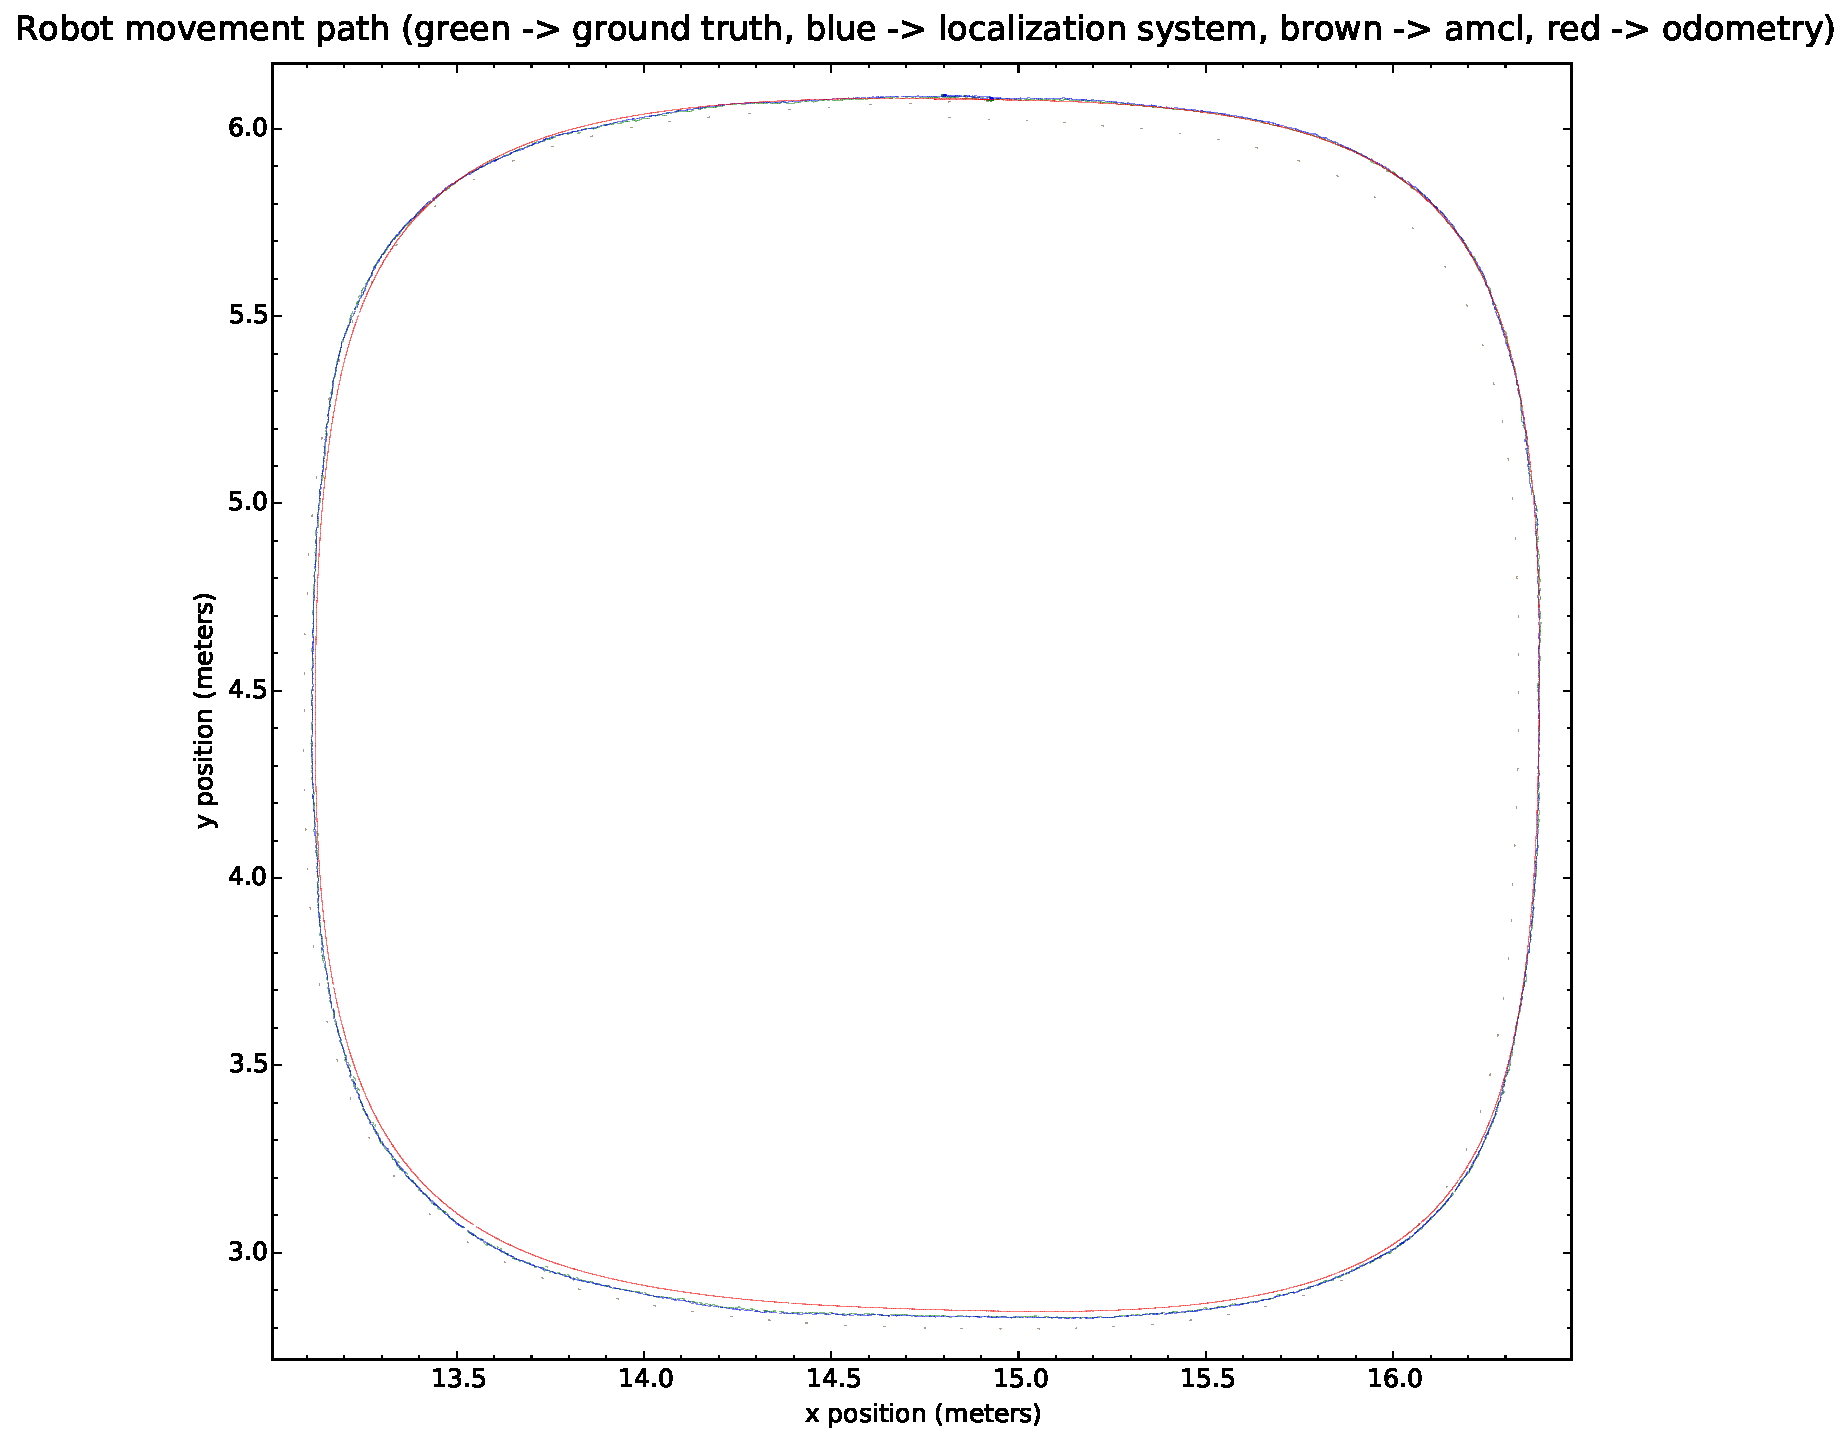
\includegraphics[width=0.8\textwidth]{appendices/tests-3dof/jarvis-robot/\currfilebase/graphs/robot-movement-path-with-odometry-and-amcl}
	\caption{Poses estimated by the ground truth, localization system, \glsentrytext{amcl} and odometry}
\end{figure}

\begin{figure}[H]
	\centering
	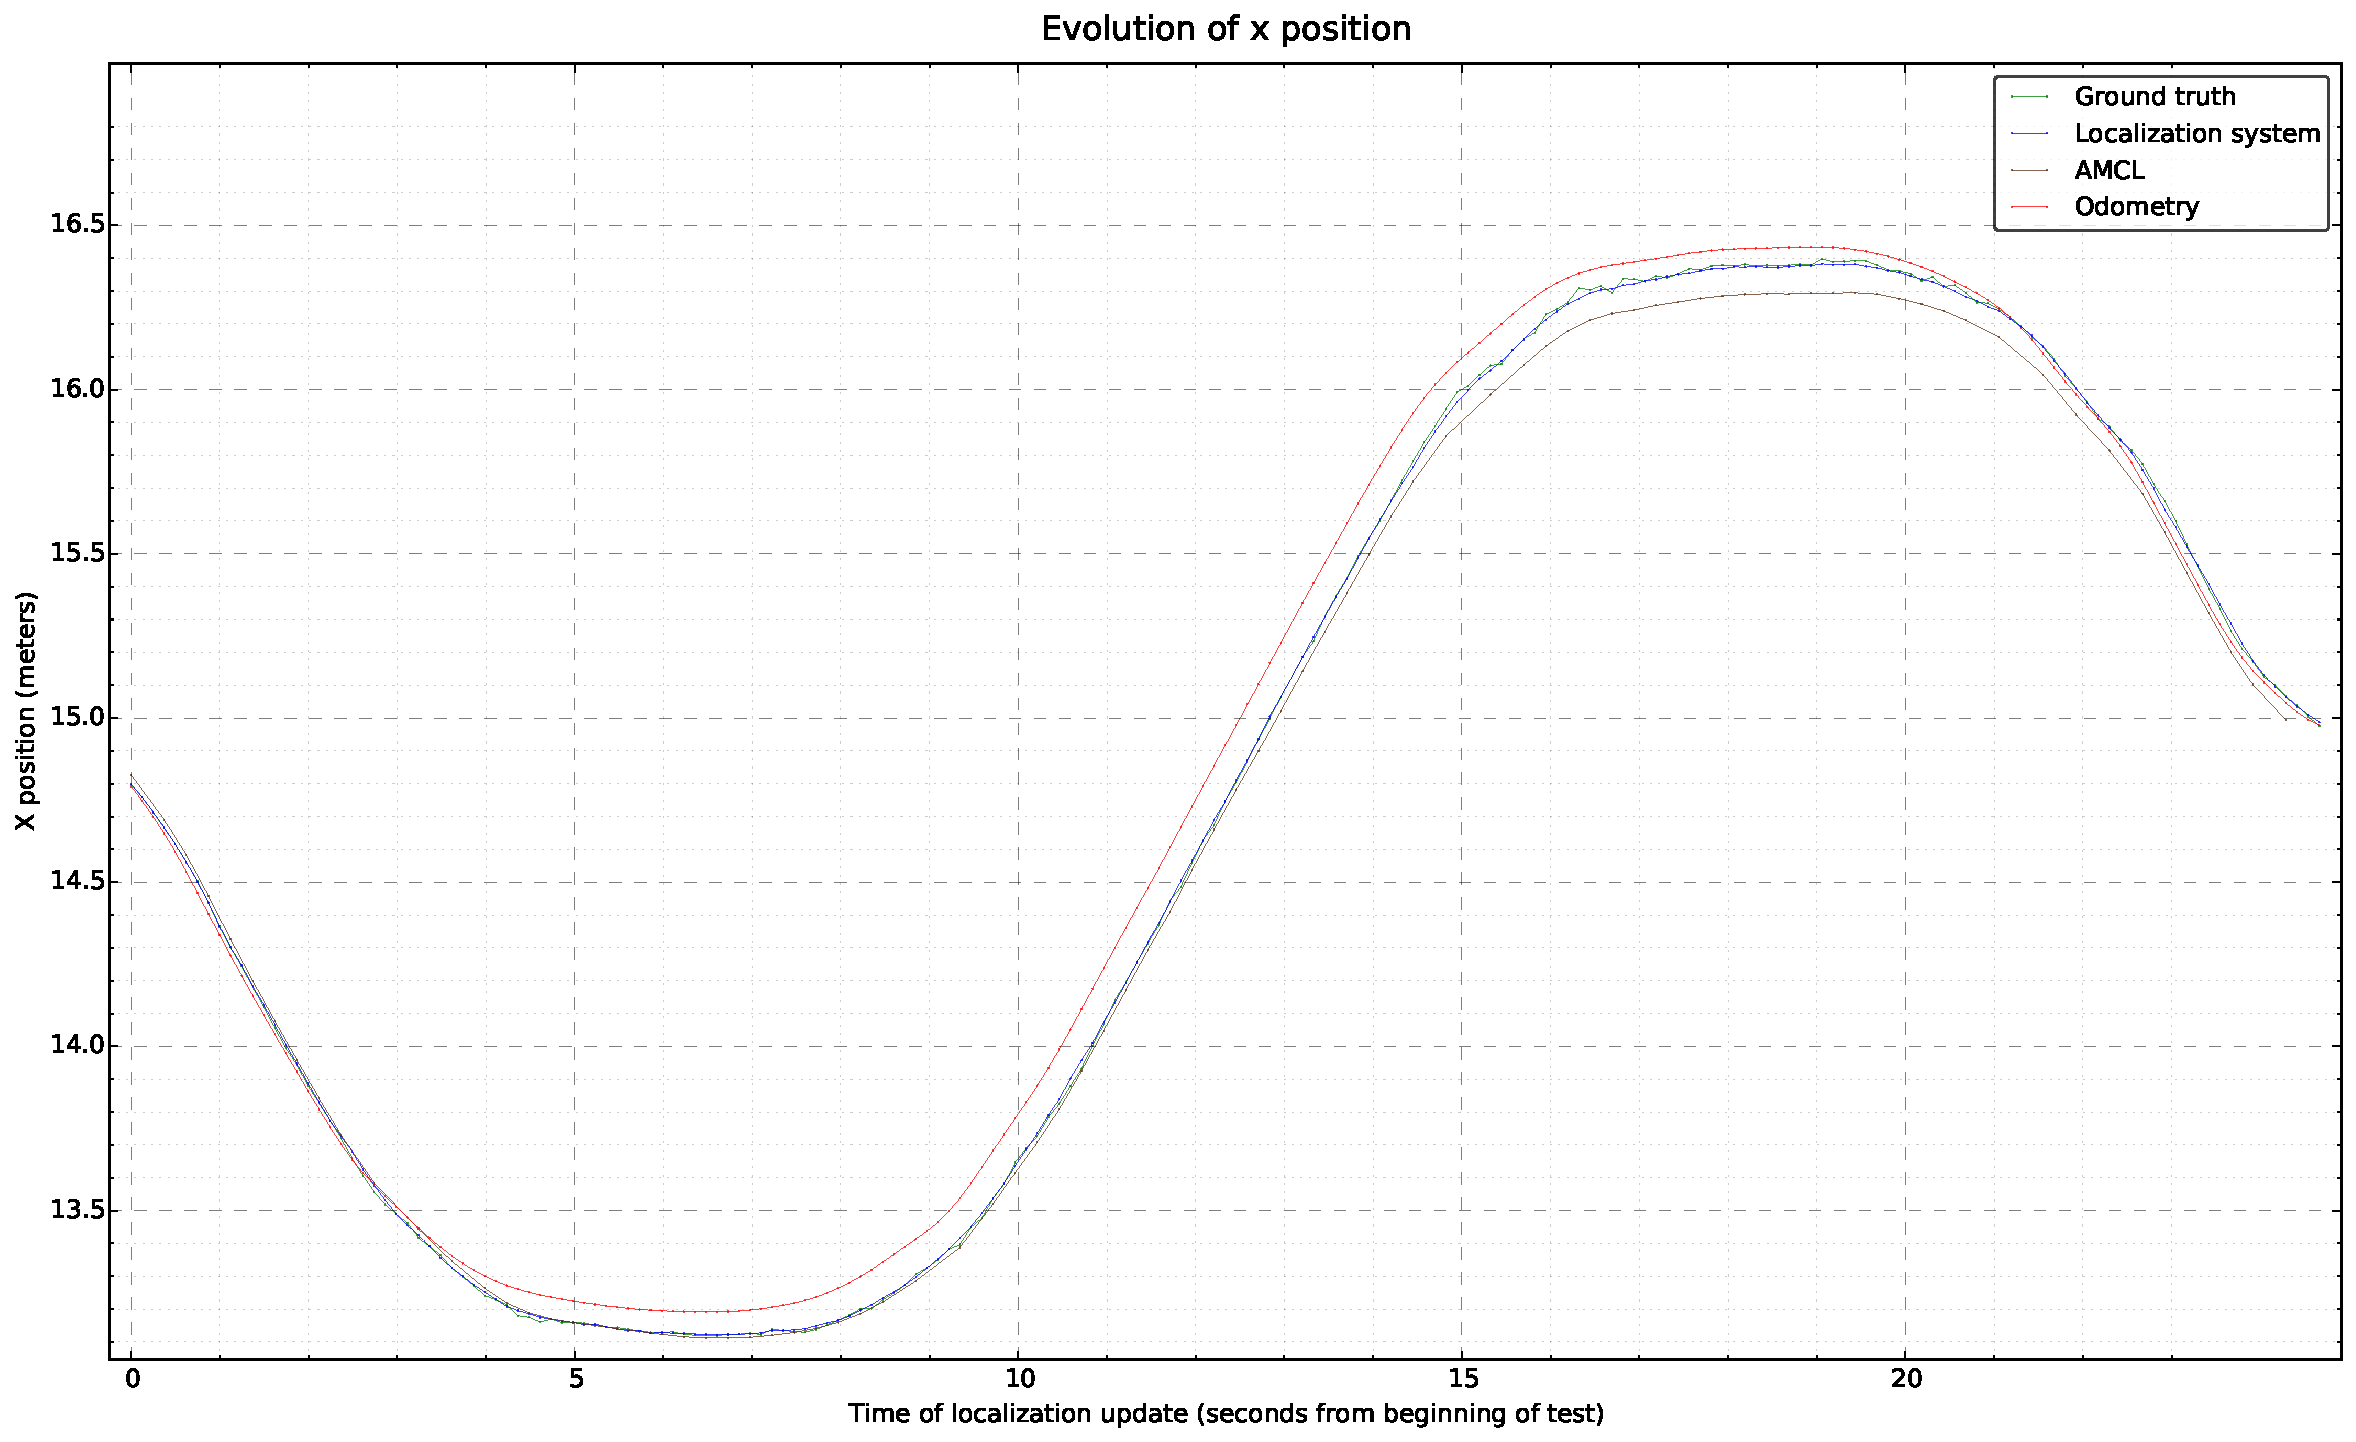
\includegraphics[width=0.53\textwidth]{appendices/tests-3dof/jarvis-robot/\currfilebase/graphs/robot-movement-path-position-evolution-x-with-amcl}
	\caption{Evolution of x position over time}
\end{figure}

\begin{figure}[H]
	\centering
	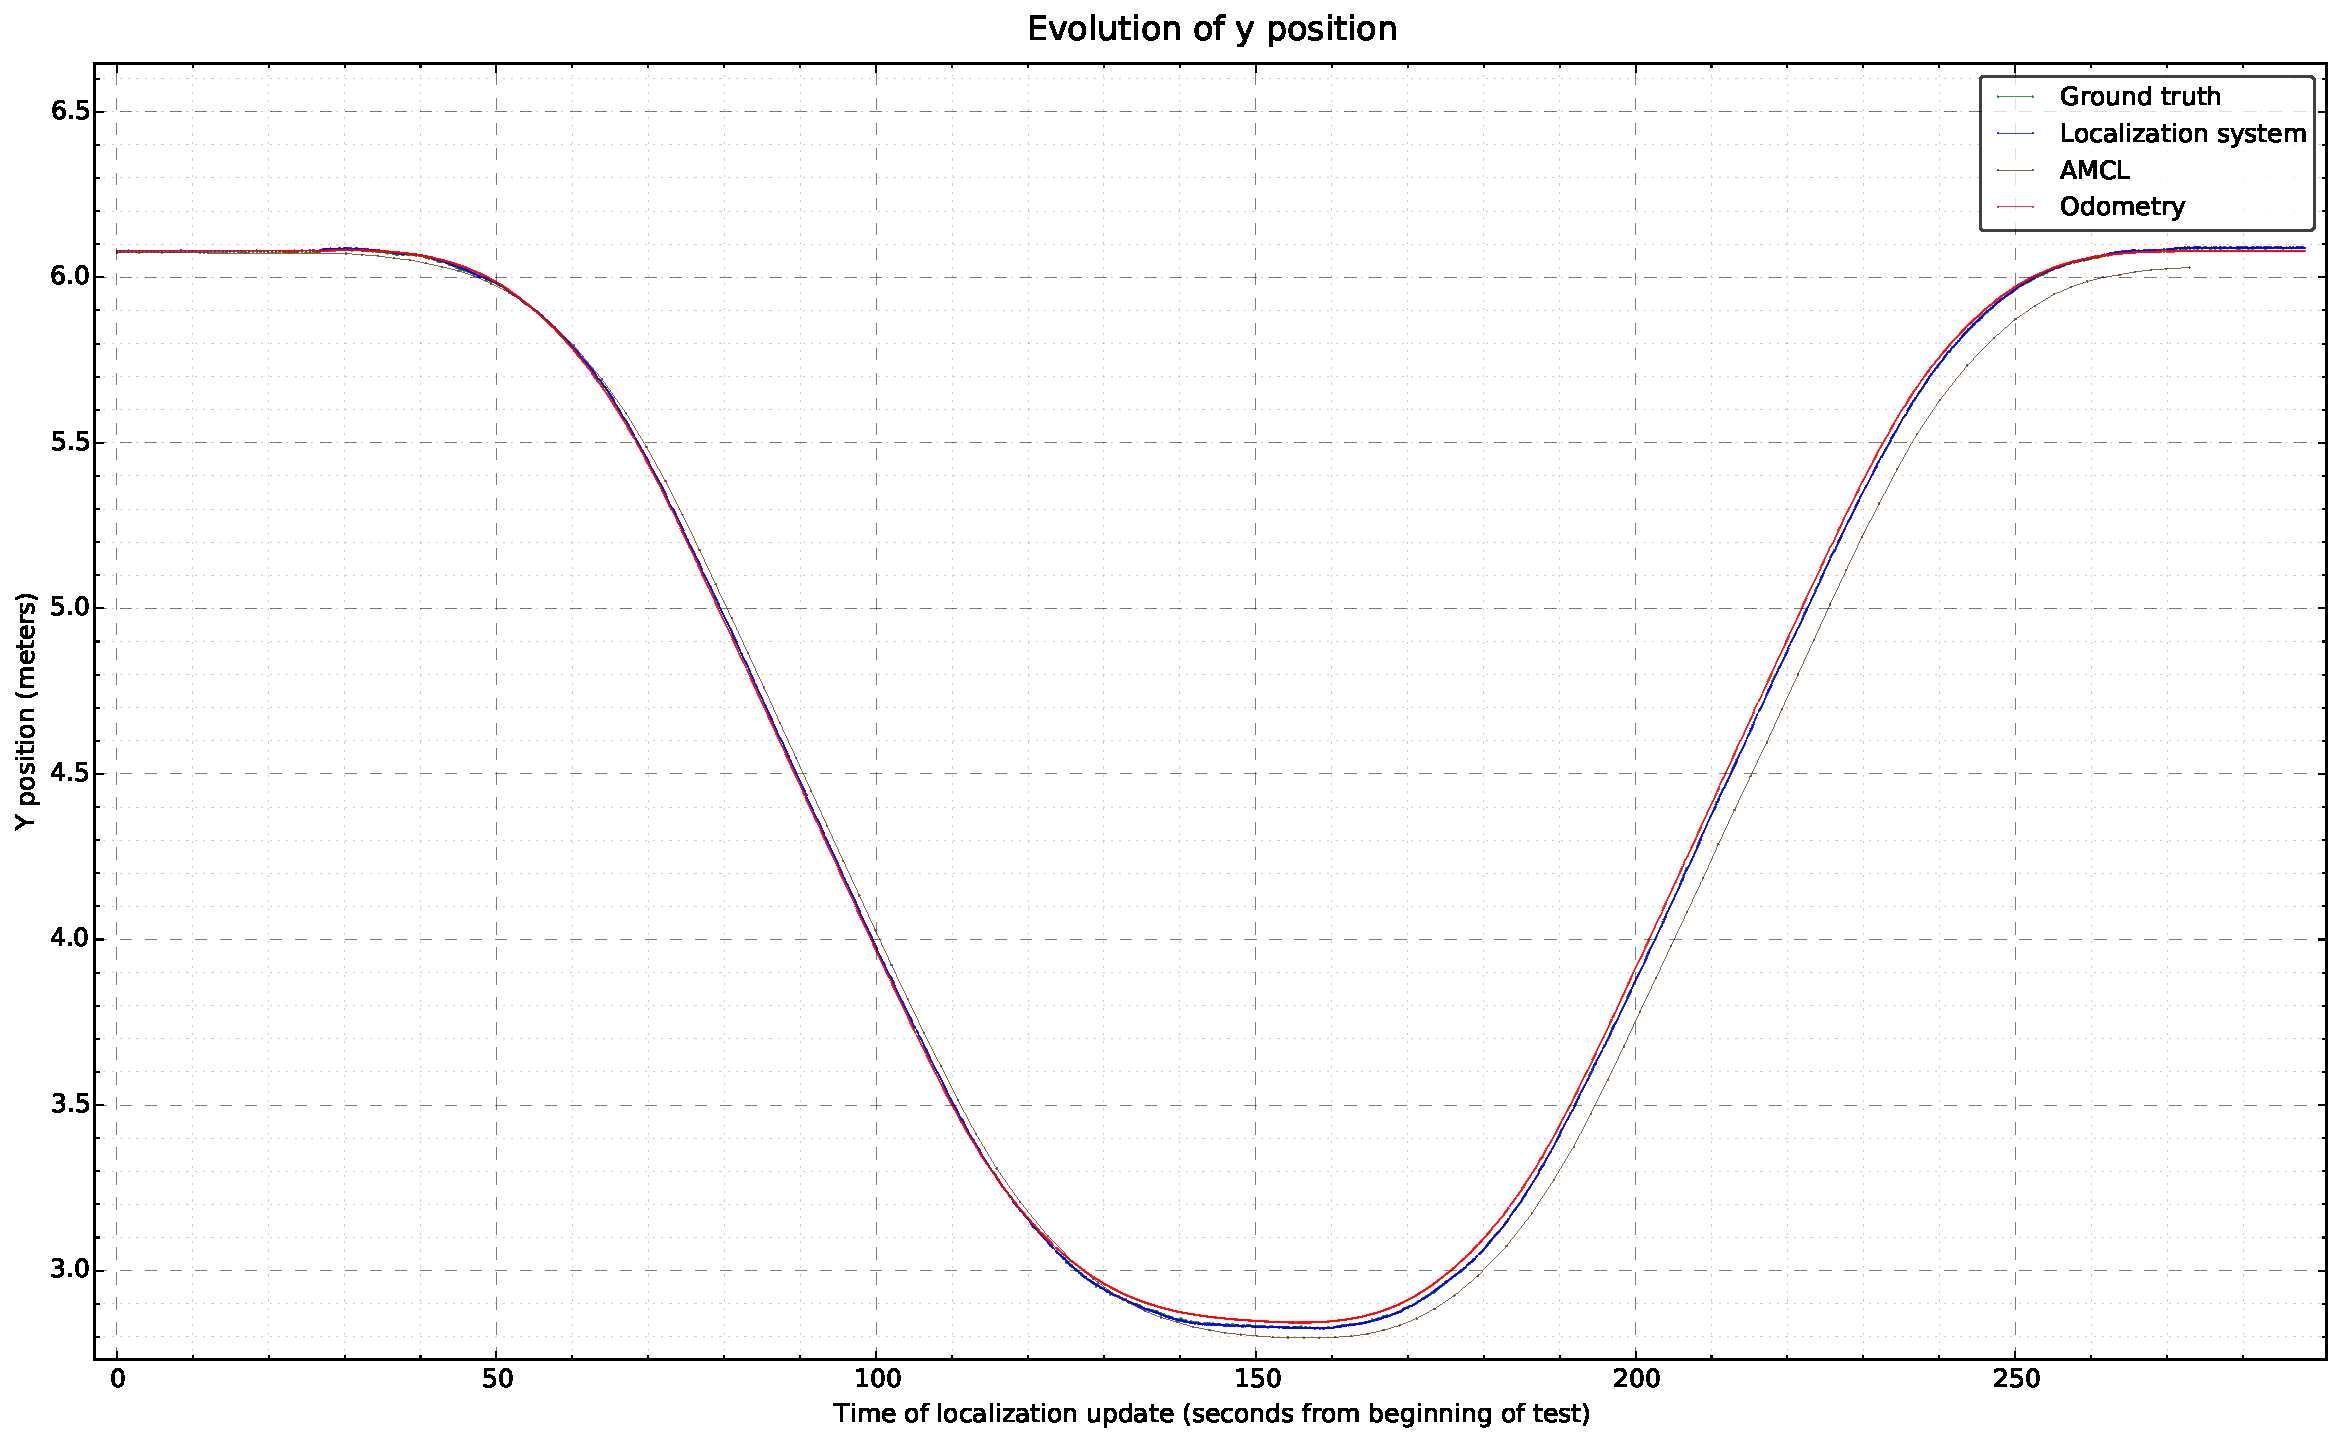
\includegraphics[width=0.53\textwidth]{appendices/tests-3dof/jarvis-robot/\currfilebase/graphs/robot-movement-path-position-evolution-y-with-amcl}
	\caption{Evolution of y position over time}
\end{figure}


%Distance derivatives
\begin{figure}[H]
	\centering
	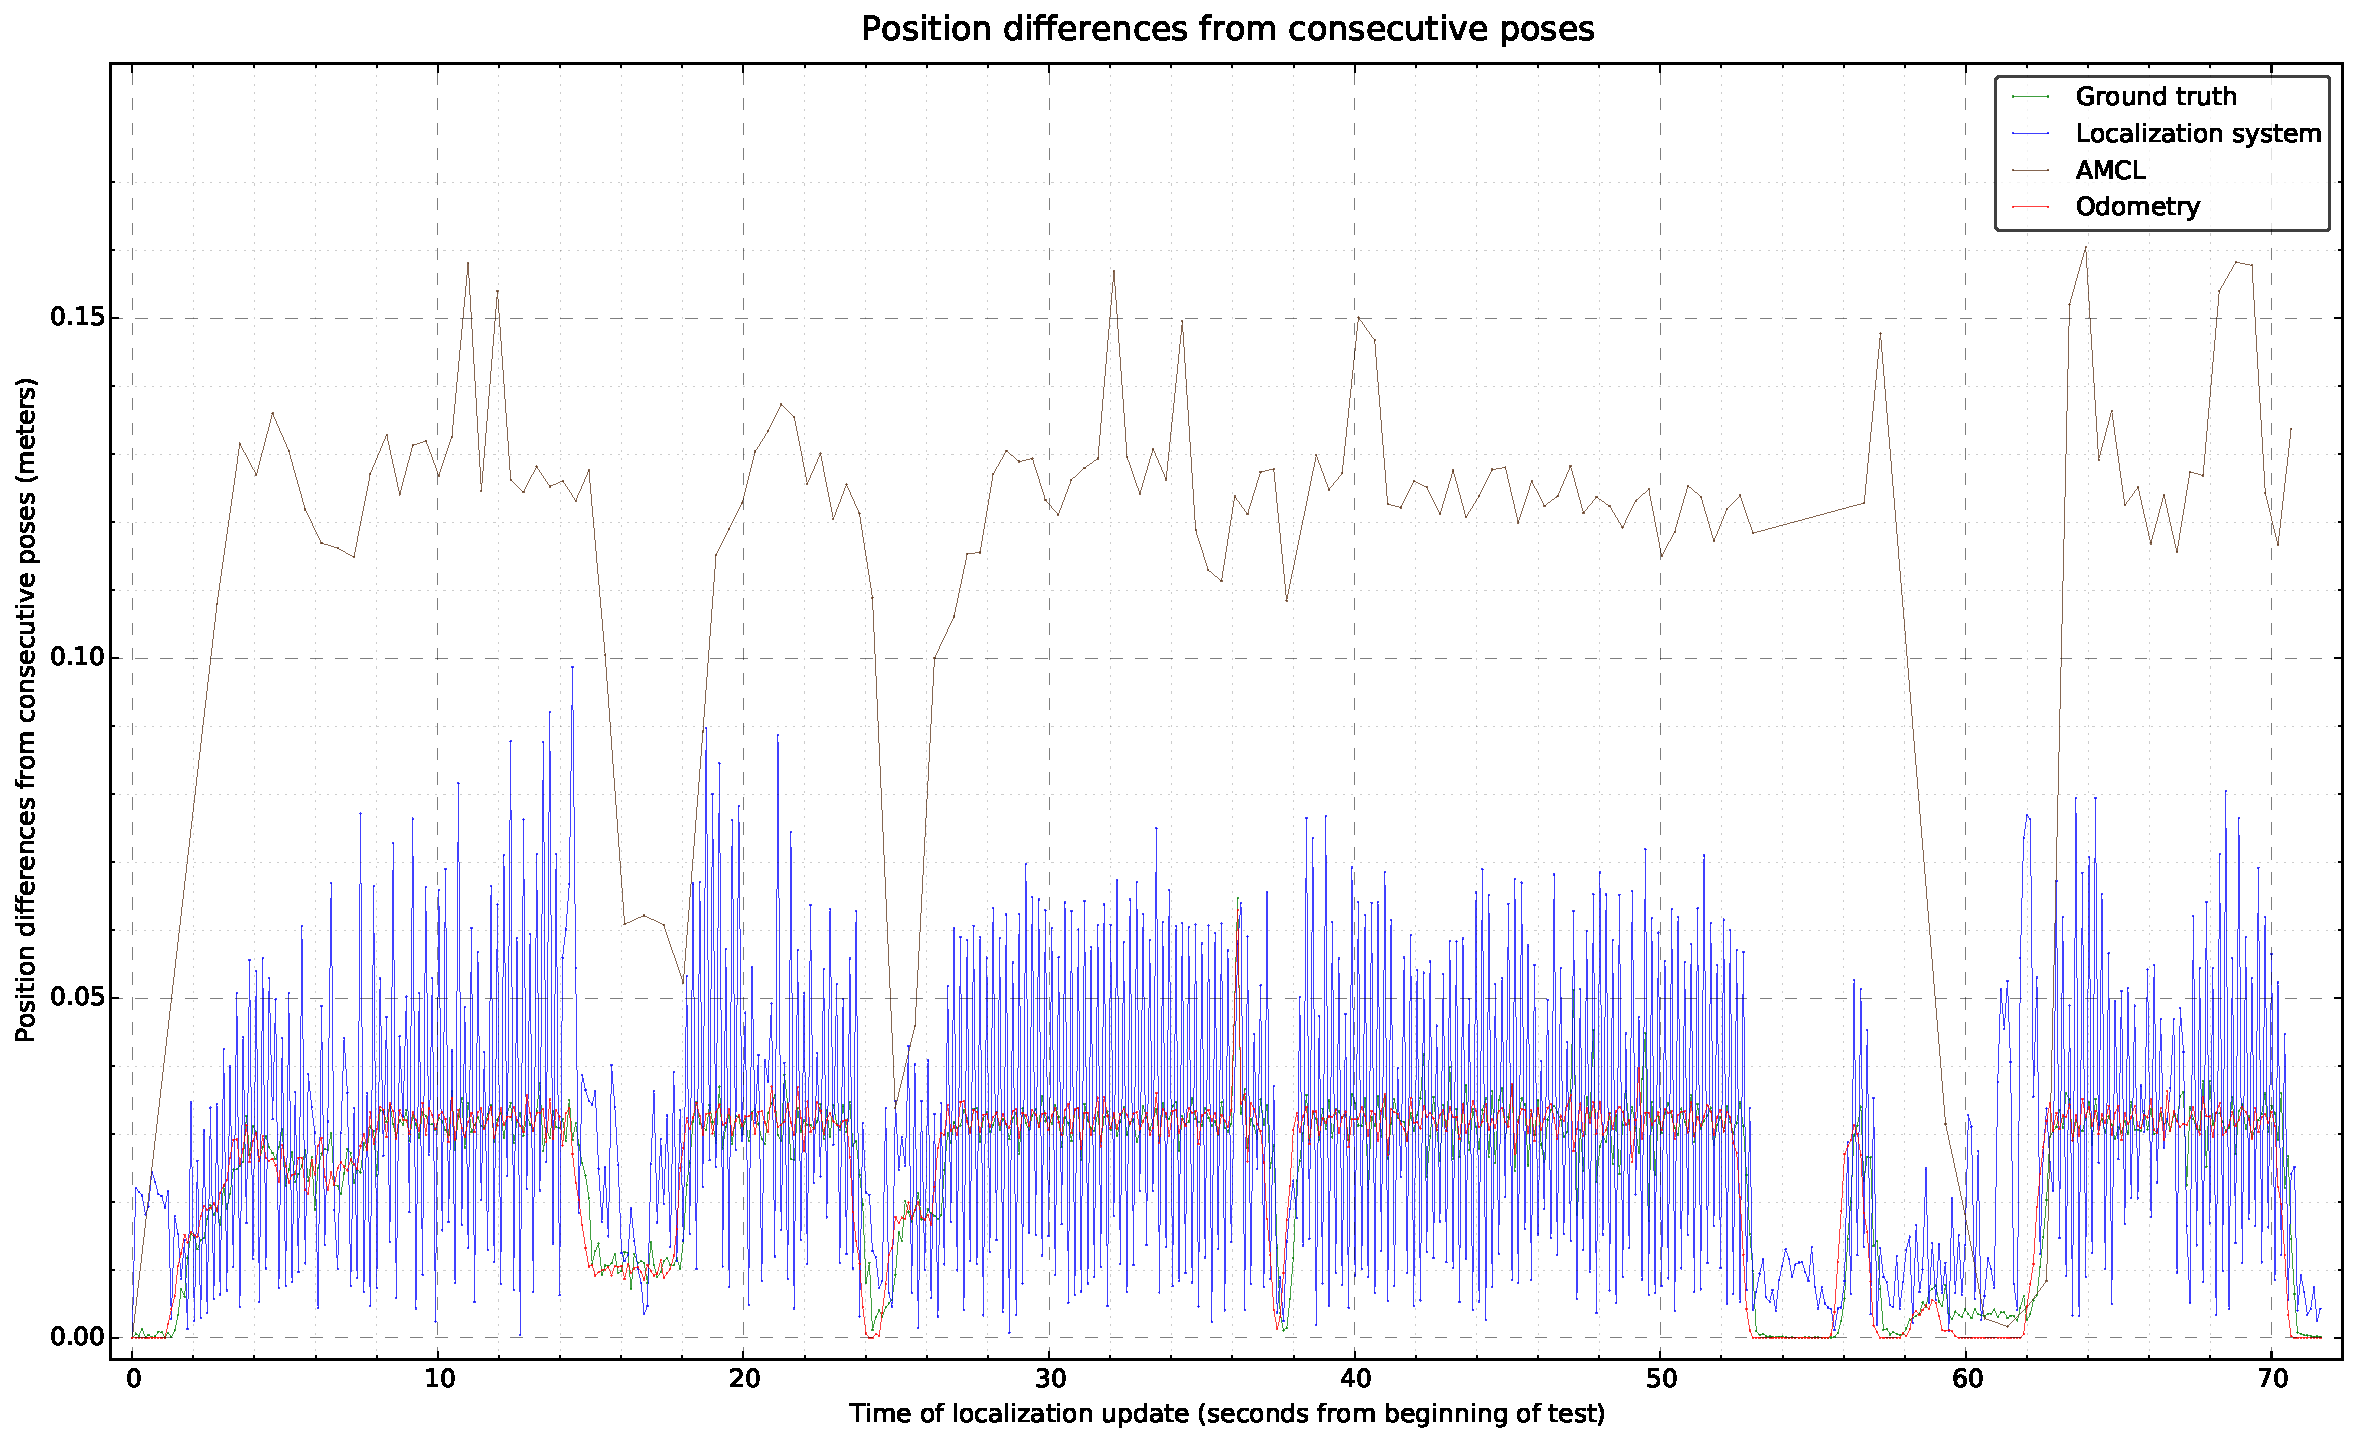
\includegraphics[width=0.7\textwidth]{appendices/tests-3dof/jarvis-robot/\currfilebase/graphs/robot-movement-path-position-differences-with-amcl}
	\caption{Distance traveled between consecutive pose estimations}
\end{figure}

\begin{figure}[H]
	\centering
	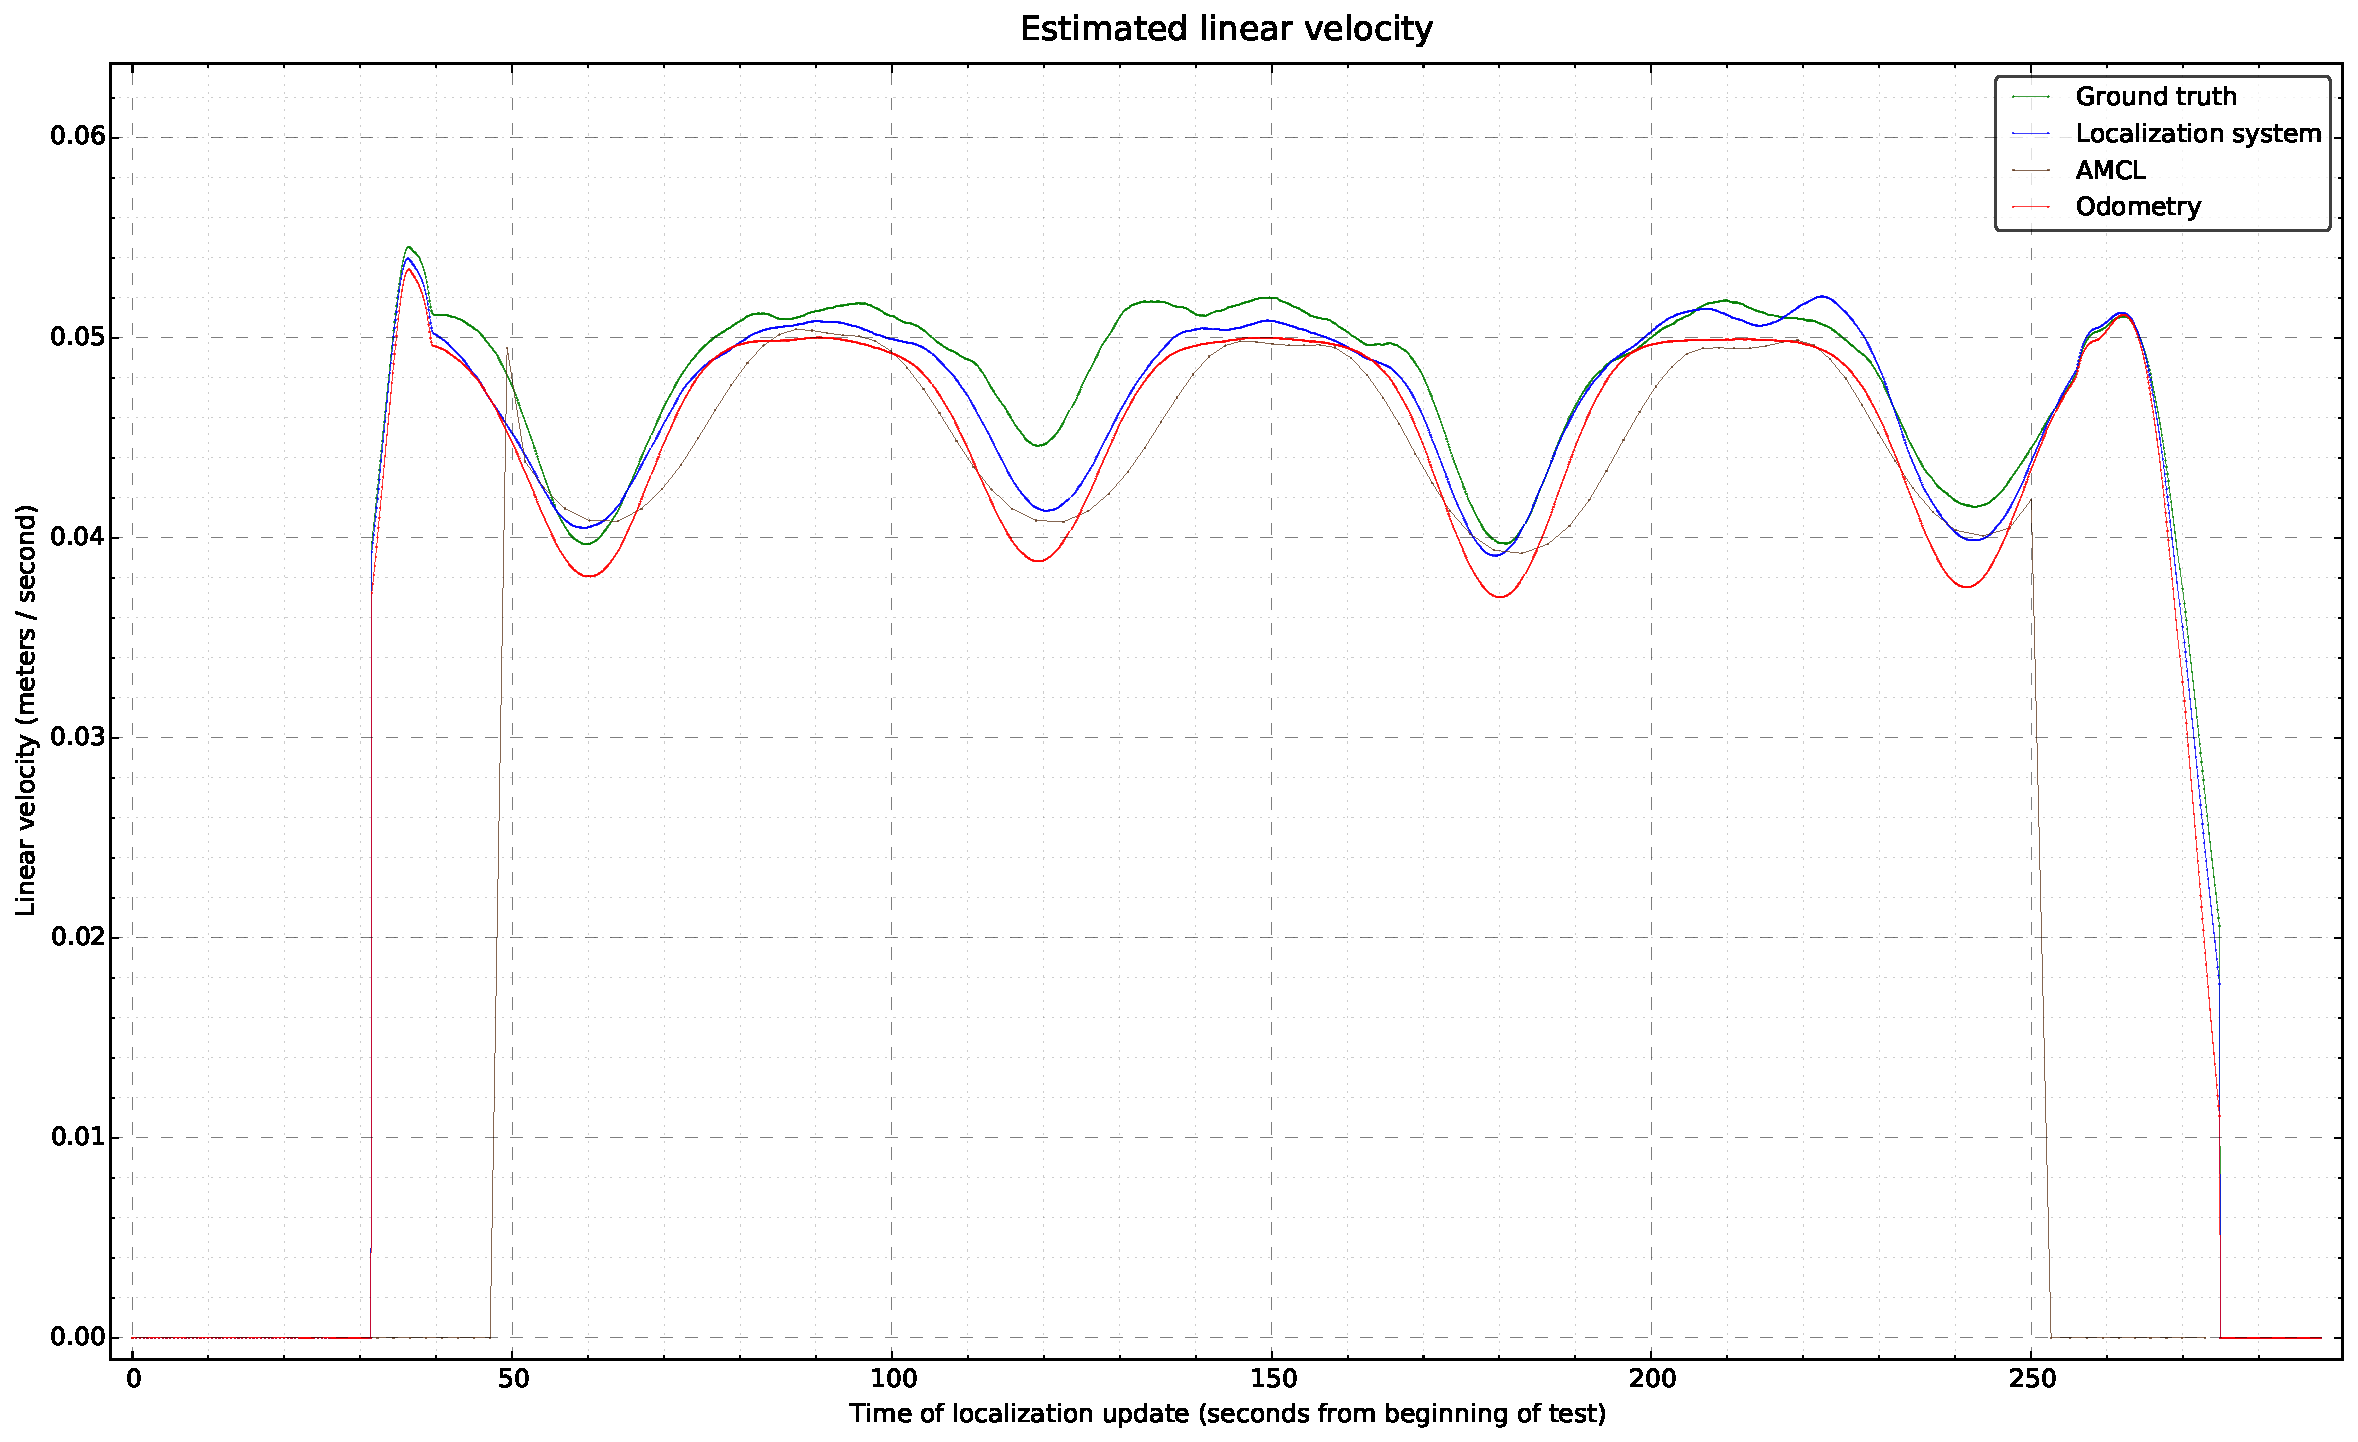
\includegraphics[width=0.7\textwidth]{appendices/tests-3dof/jarvis-robot/\currfilebase/graphs/robot-movement-path-linear-velocity-with-amcl}
	\caption{Estimated linear velocity}
\end{figure}

\begin{figure}[H]
	\centering
	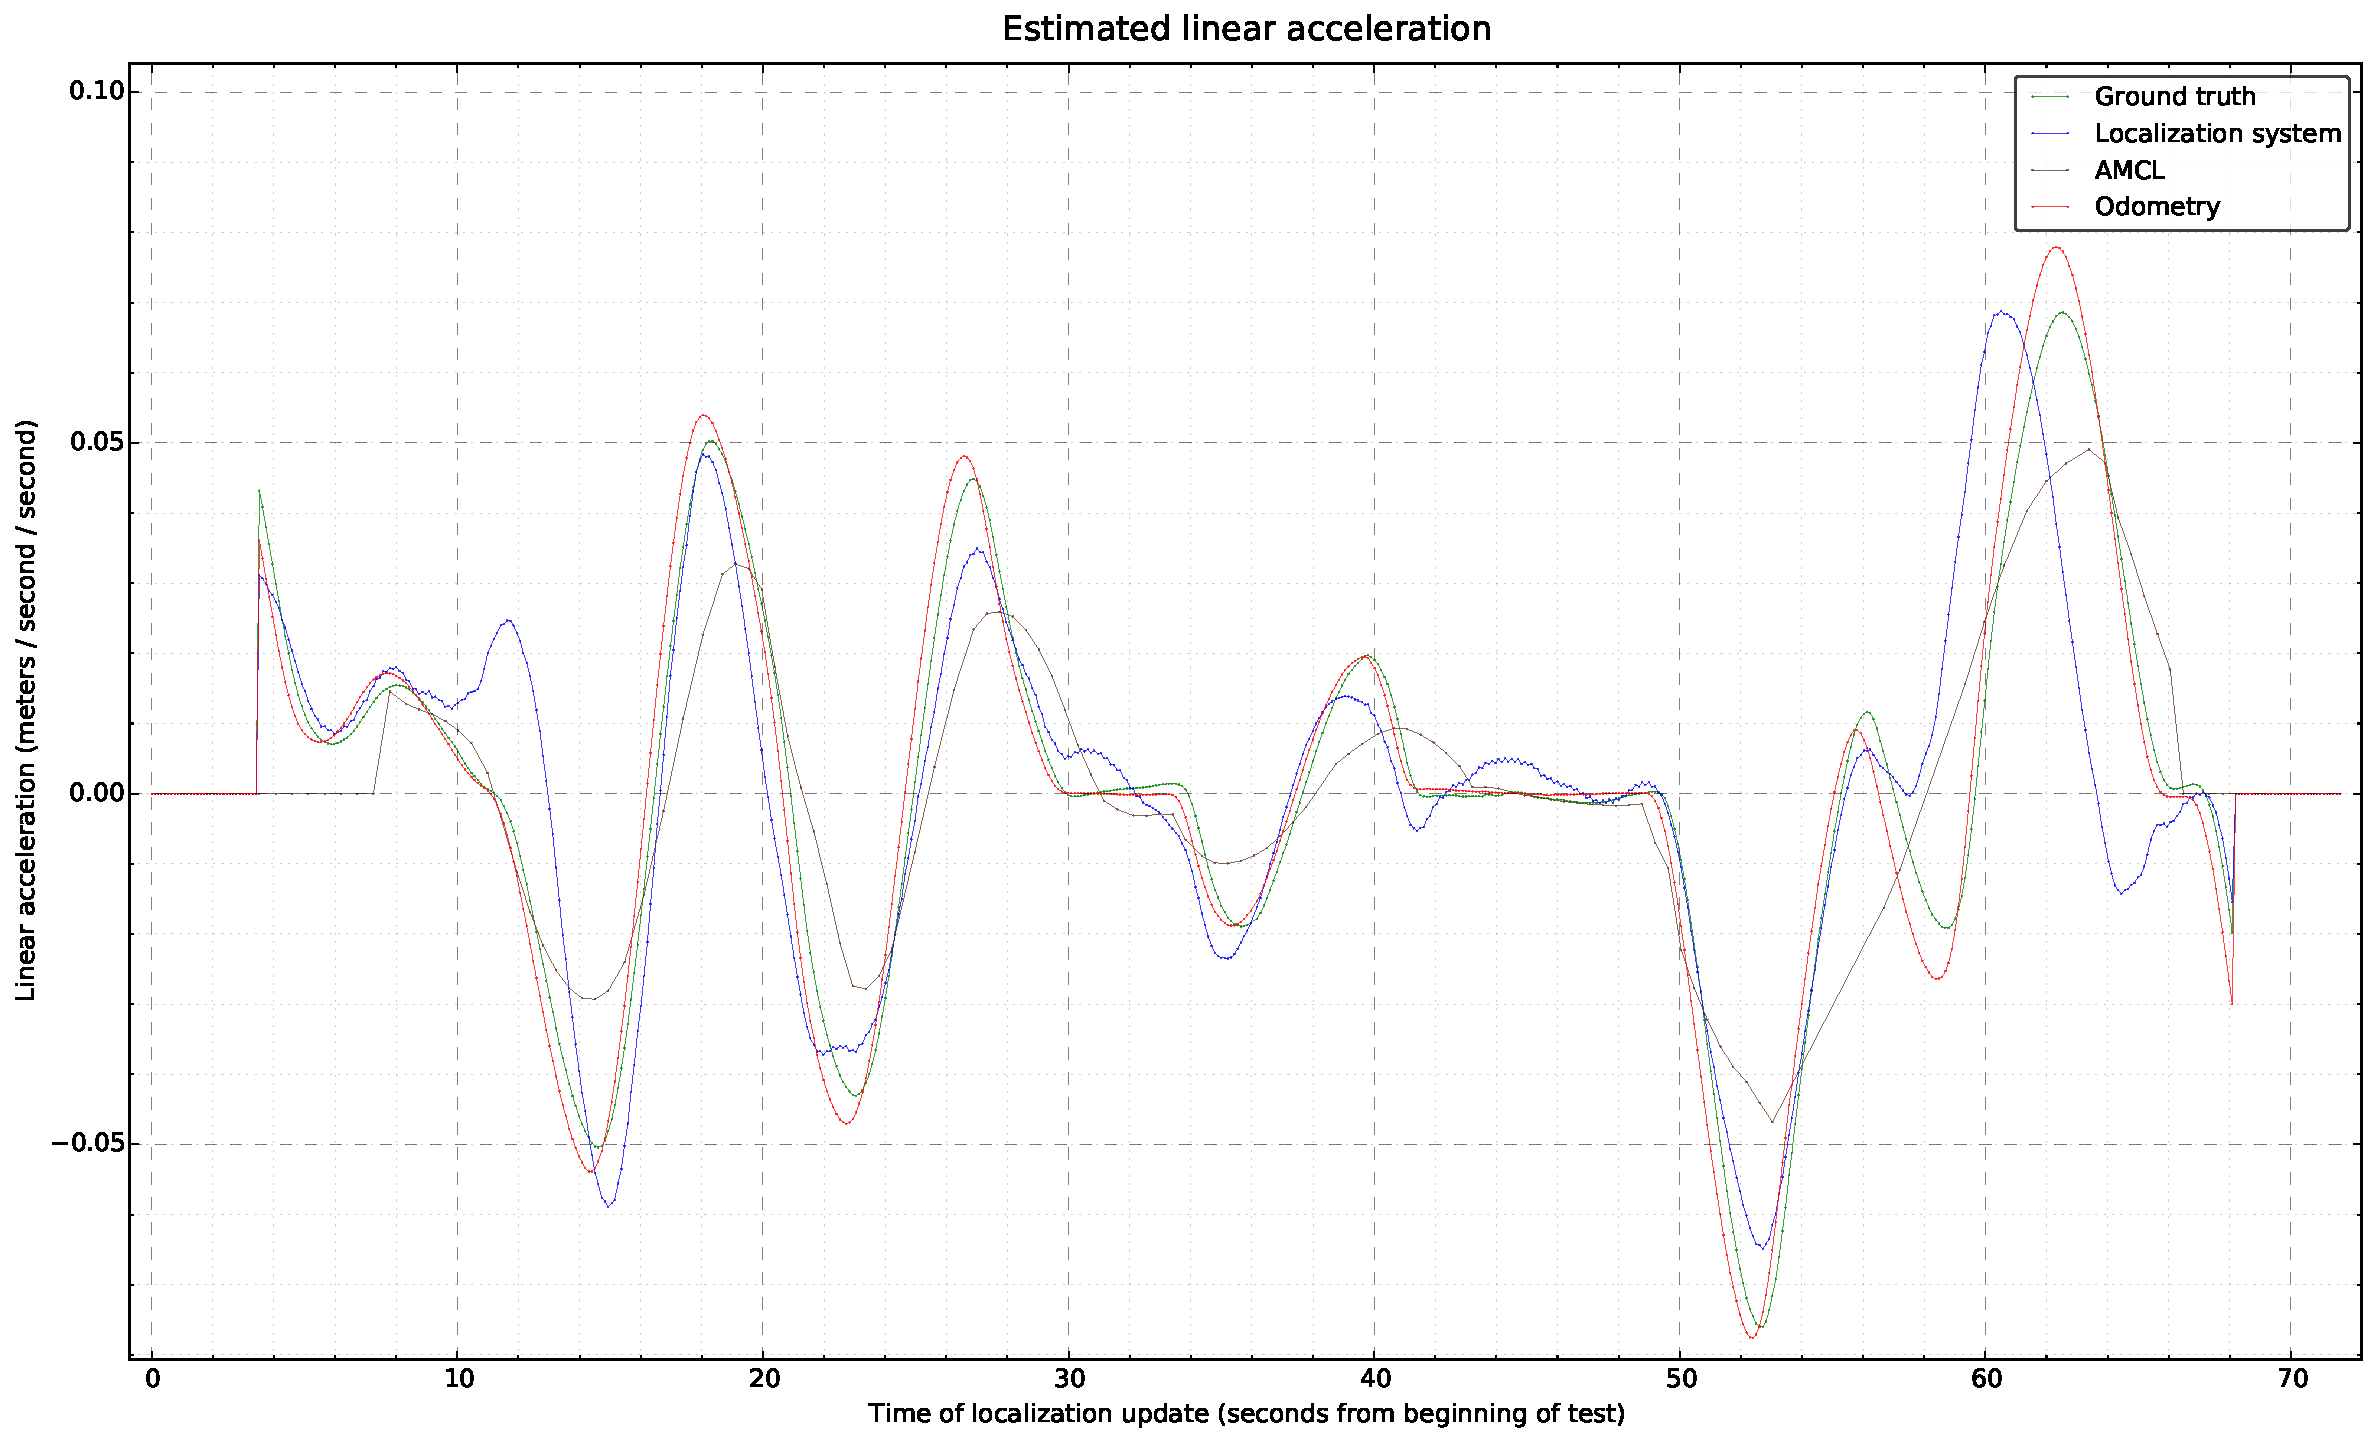
\includegraphics[width=0.7\textwidth]{appendices/tests-3dof/jarvis-robot/\currfilebase/graphs/robot-movement-path-linear-acceleration-with-amcl}
	\caption{Estimated linear acceleration}
\end{figure}


%Angular derivatives
\begin{figure}[H]
	\centering
	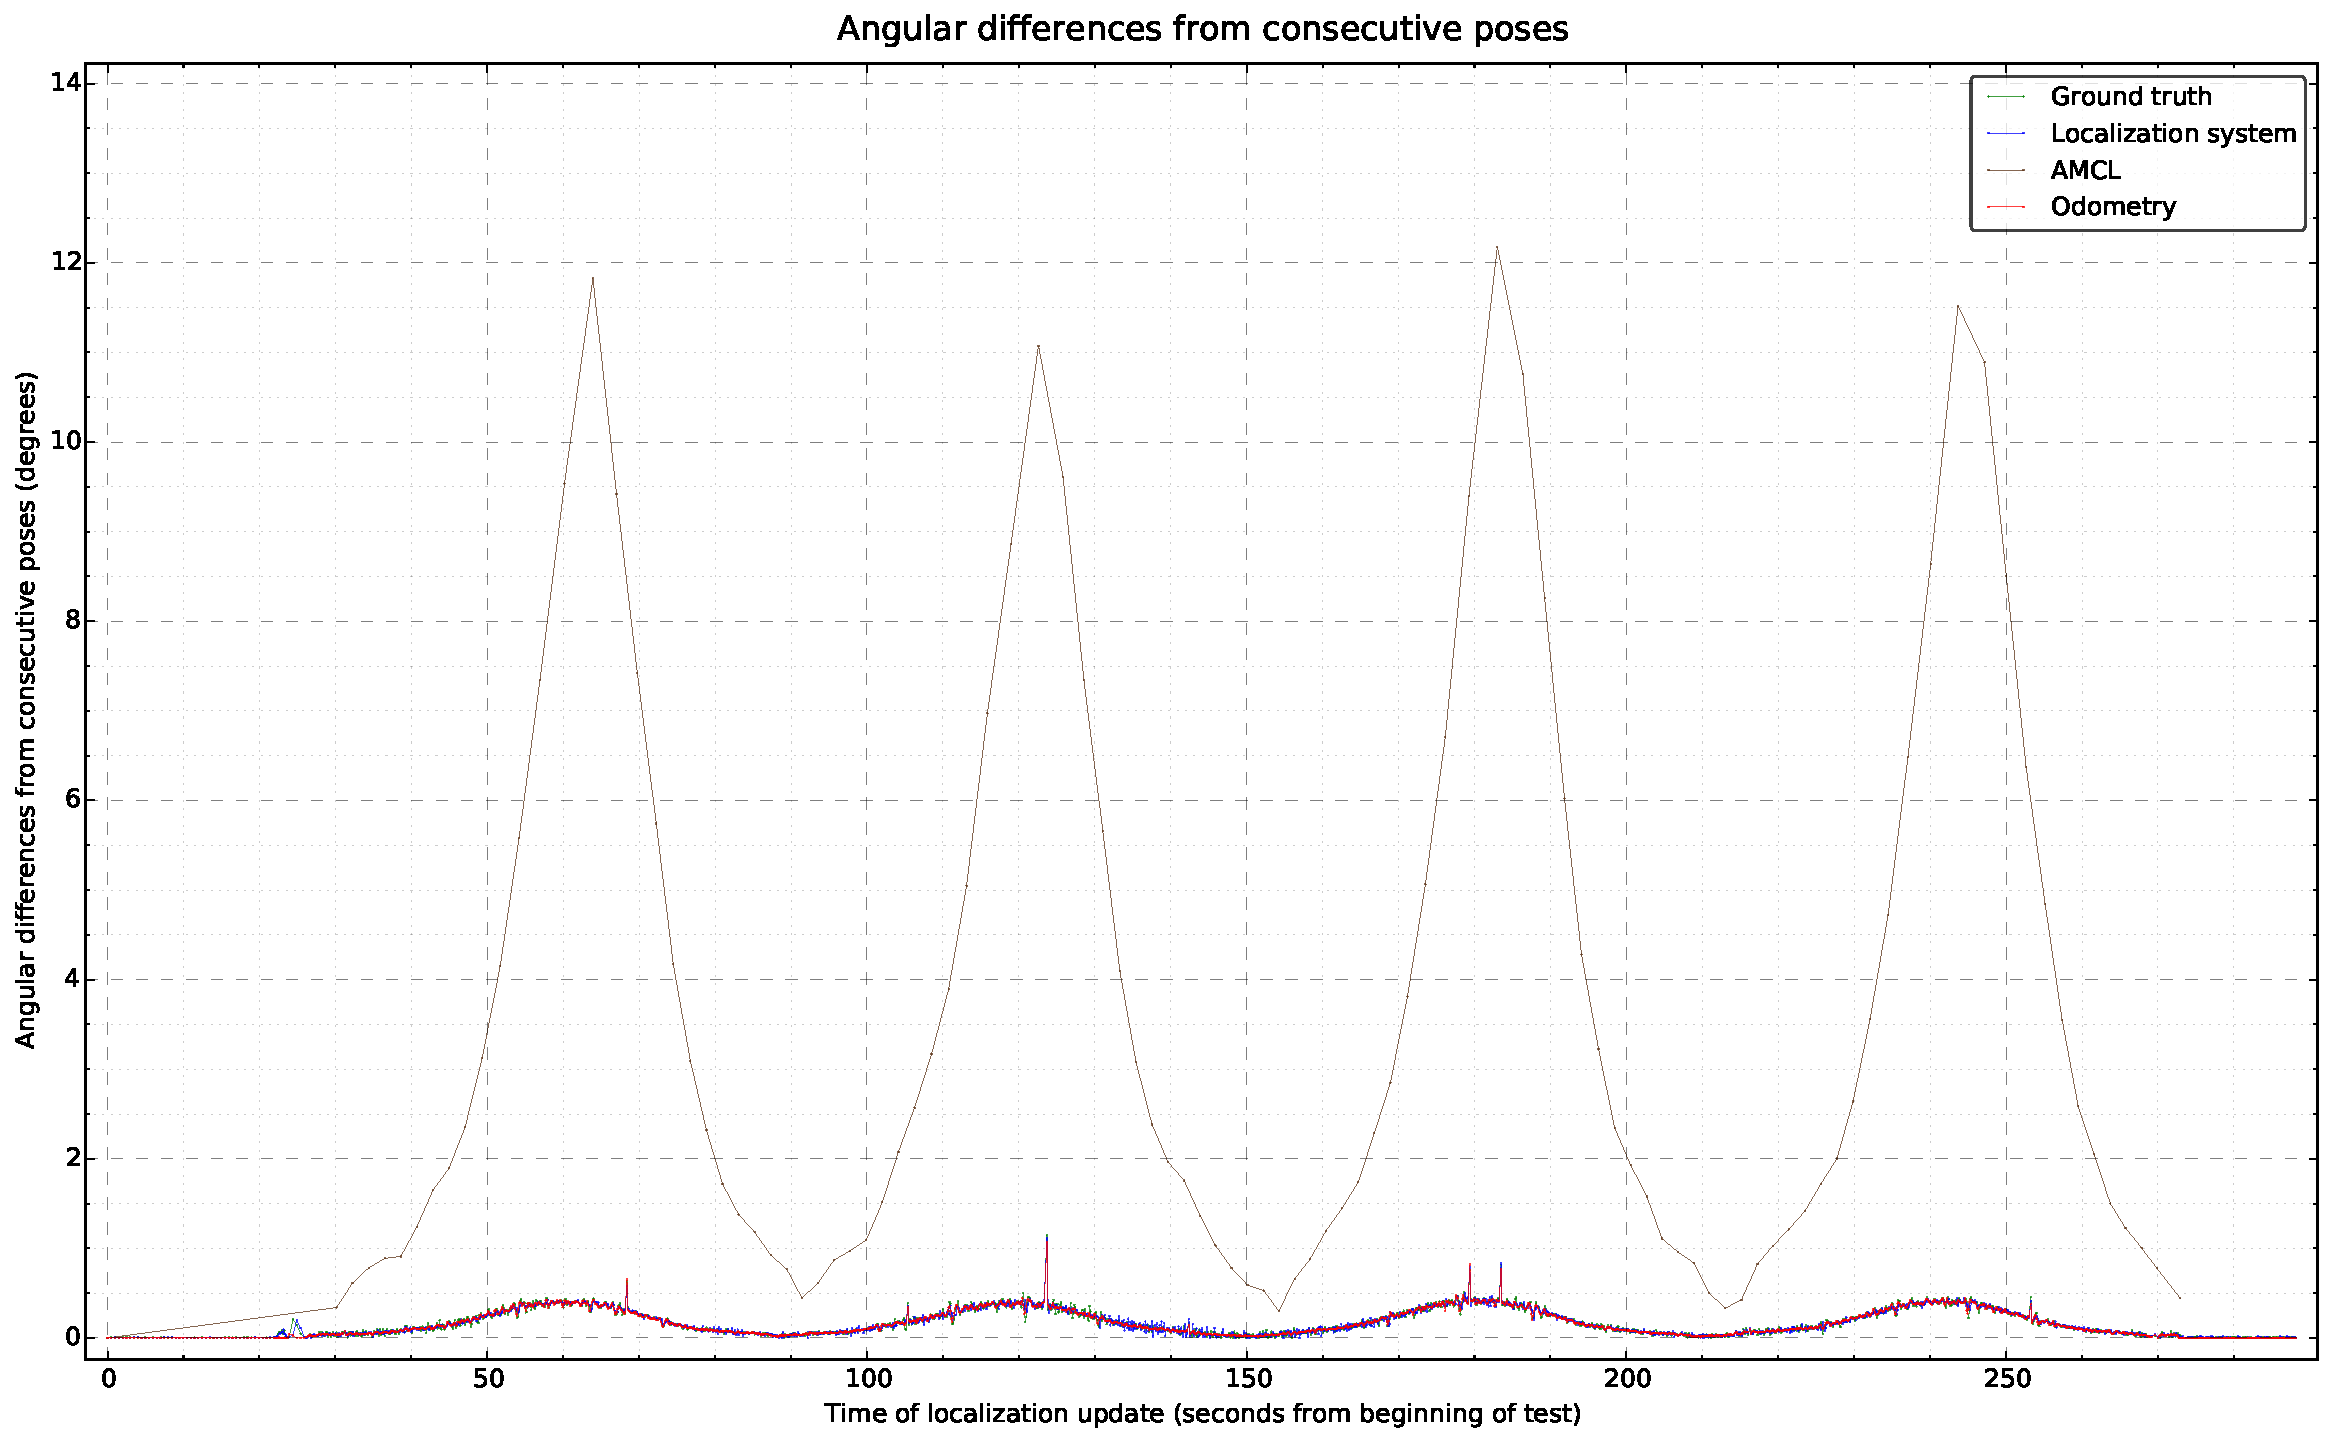
\includegraphics[width=0.69\textwidth]{appendices/tests-3dof/jarvis-robot/\currfilebase/graphs/robot-movement-path-angular-differences-with-amcl}
	\caption{Angular differences between consecutive pose estimations}
\end{figure}

\begin{figure}[H]
	\centering
	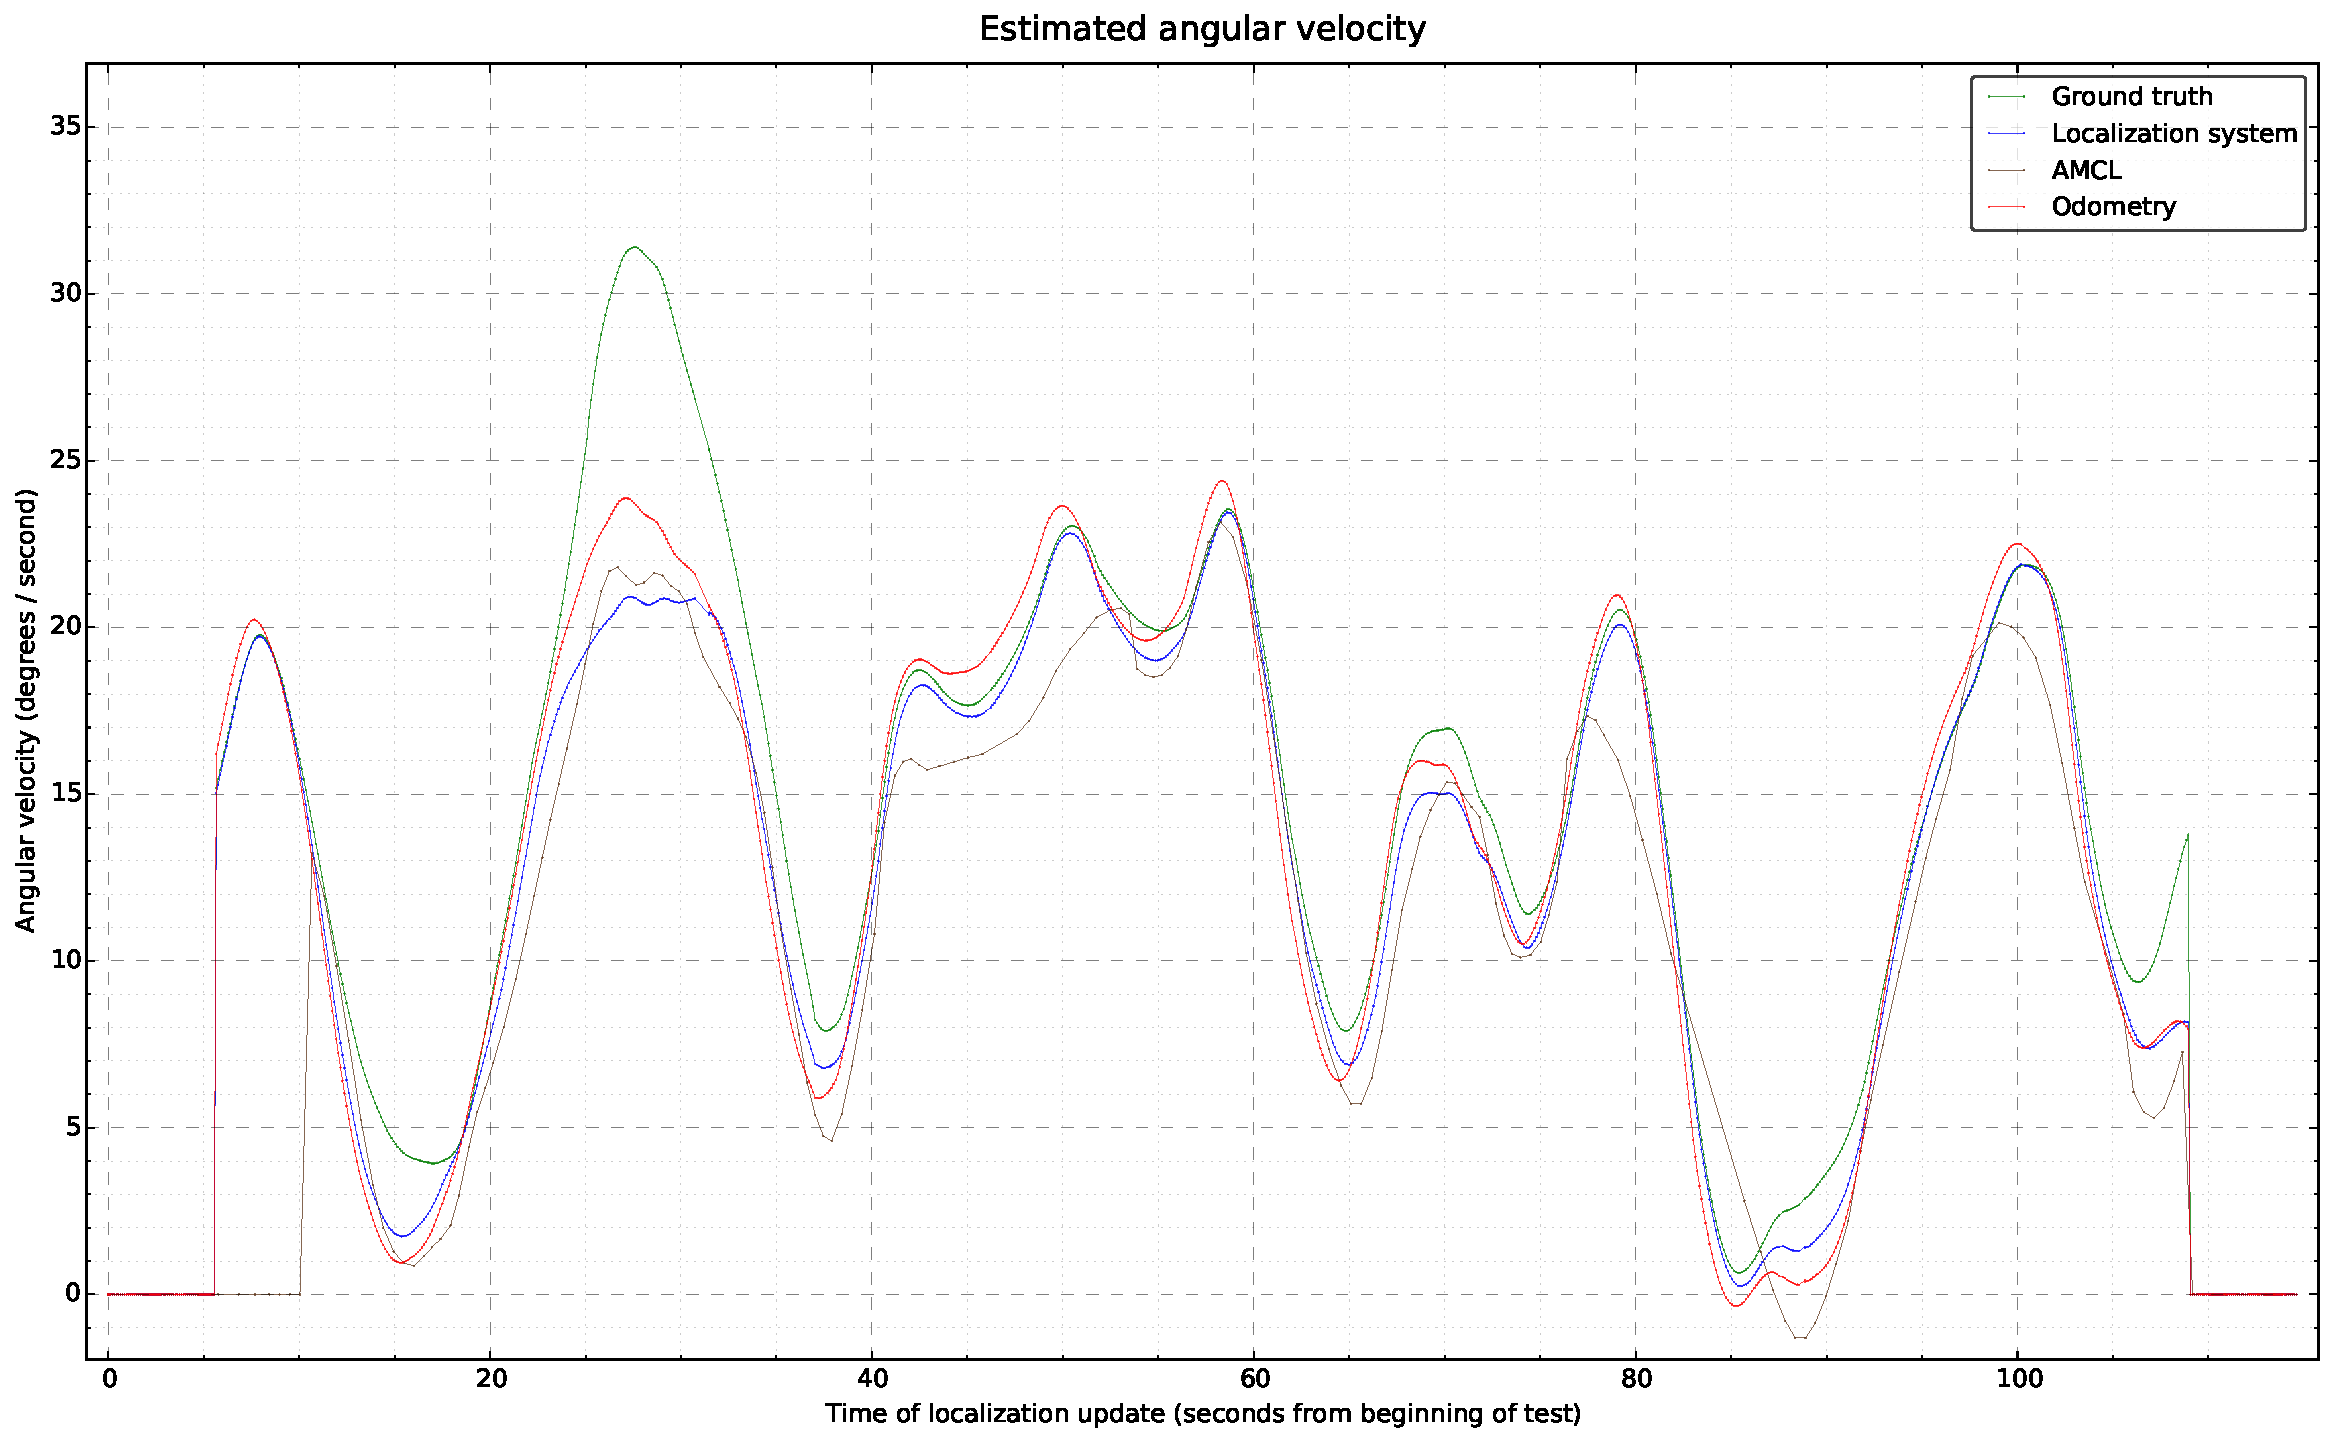
\includegraphics[width=0.69\textwidth]{appendices/tests-3dof/jarvis-robot/\currfilebase/graphs/robot-movement-path-angular-velocity-with-amcl}
	\caption{Estimated angular velocity}
\end{figure}

\begin{figure}[H]
	\centering
	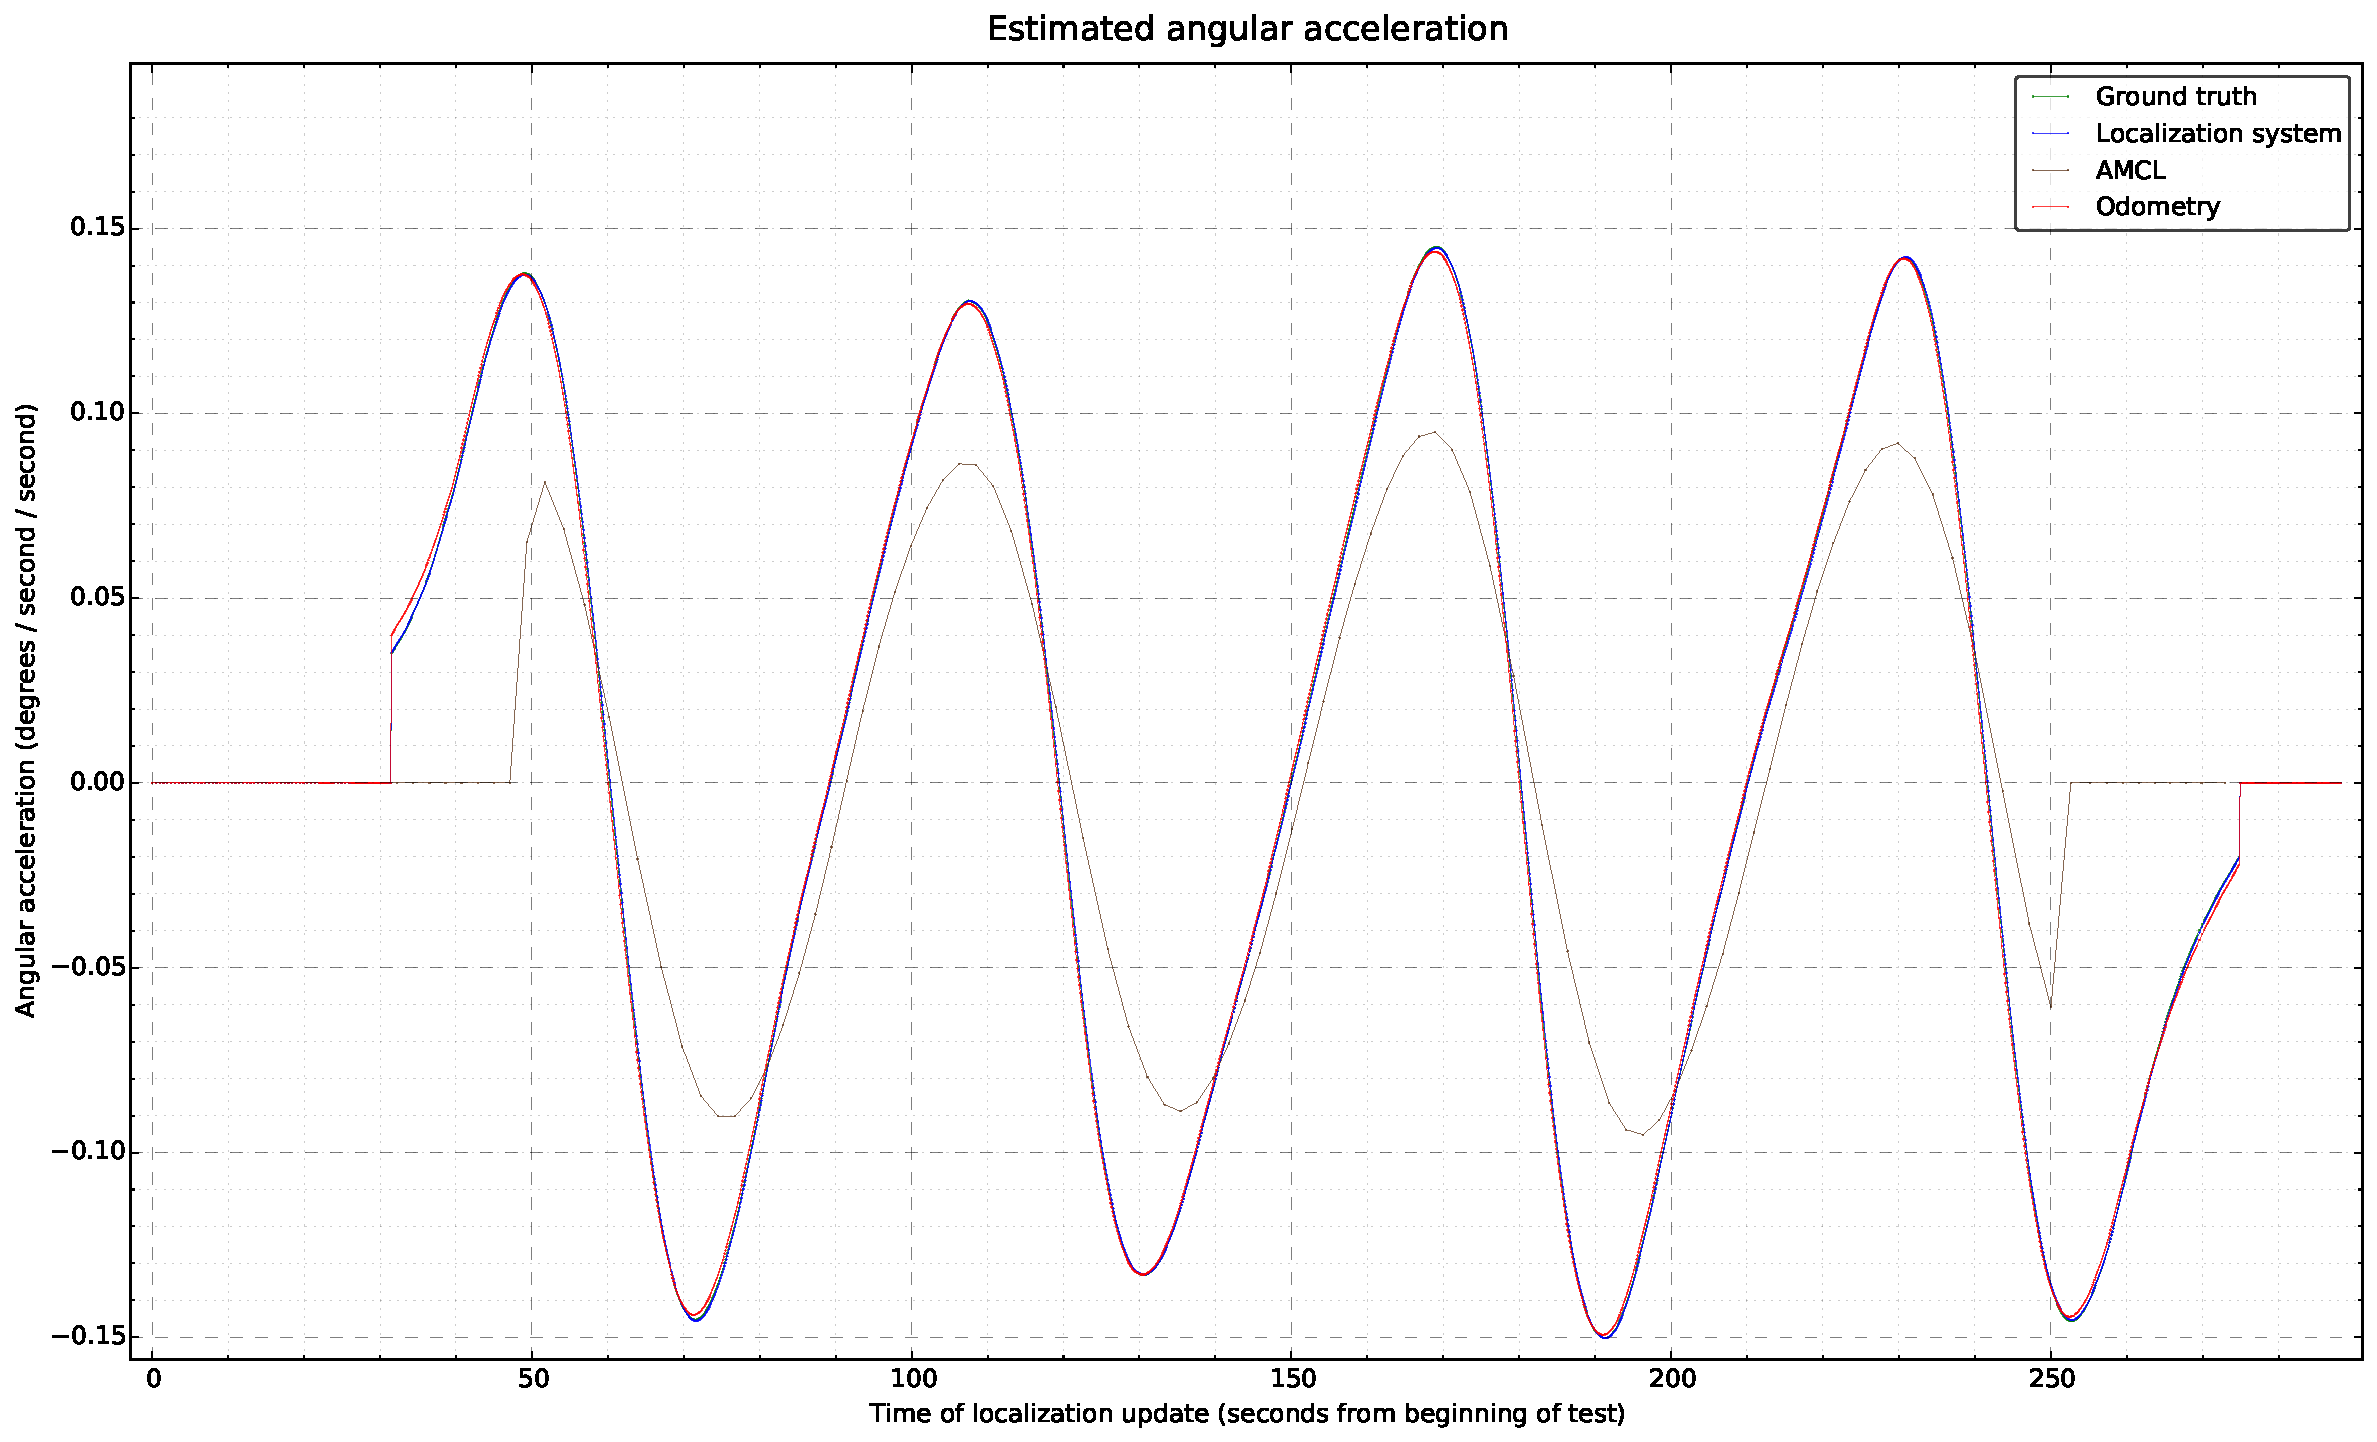
\includegraphics[width=0.69\textwidth]{appendices/tests-3dof/jarvis-robot/\currfilebase/graphs/robot-movement-path-angular-acceleration-with-amcl}
	\caption{Estimated angular acceleration}
\end{figure}


%Translation errors
\begin{figure}[H]
	\centering
	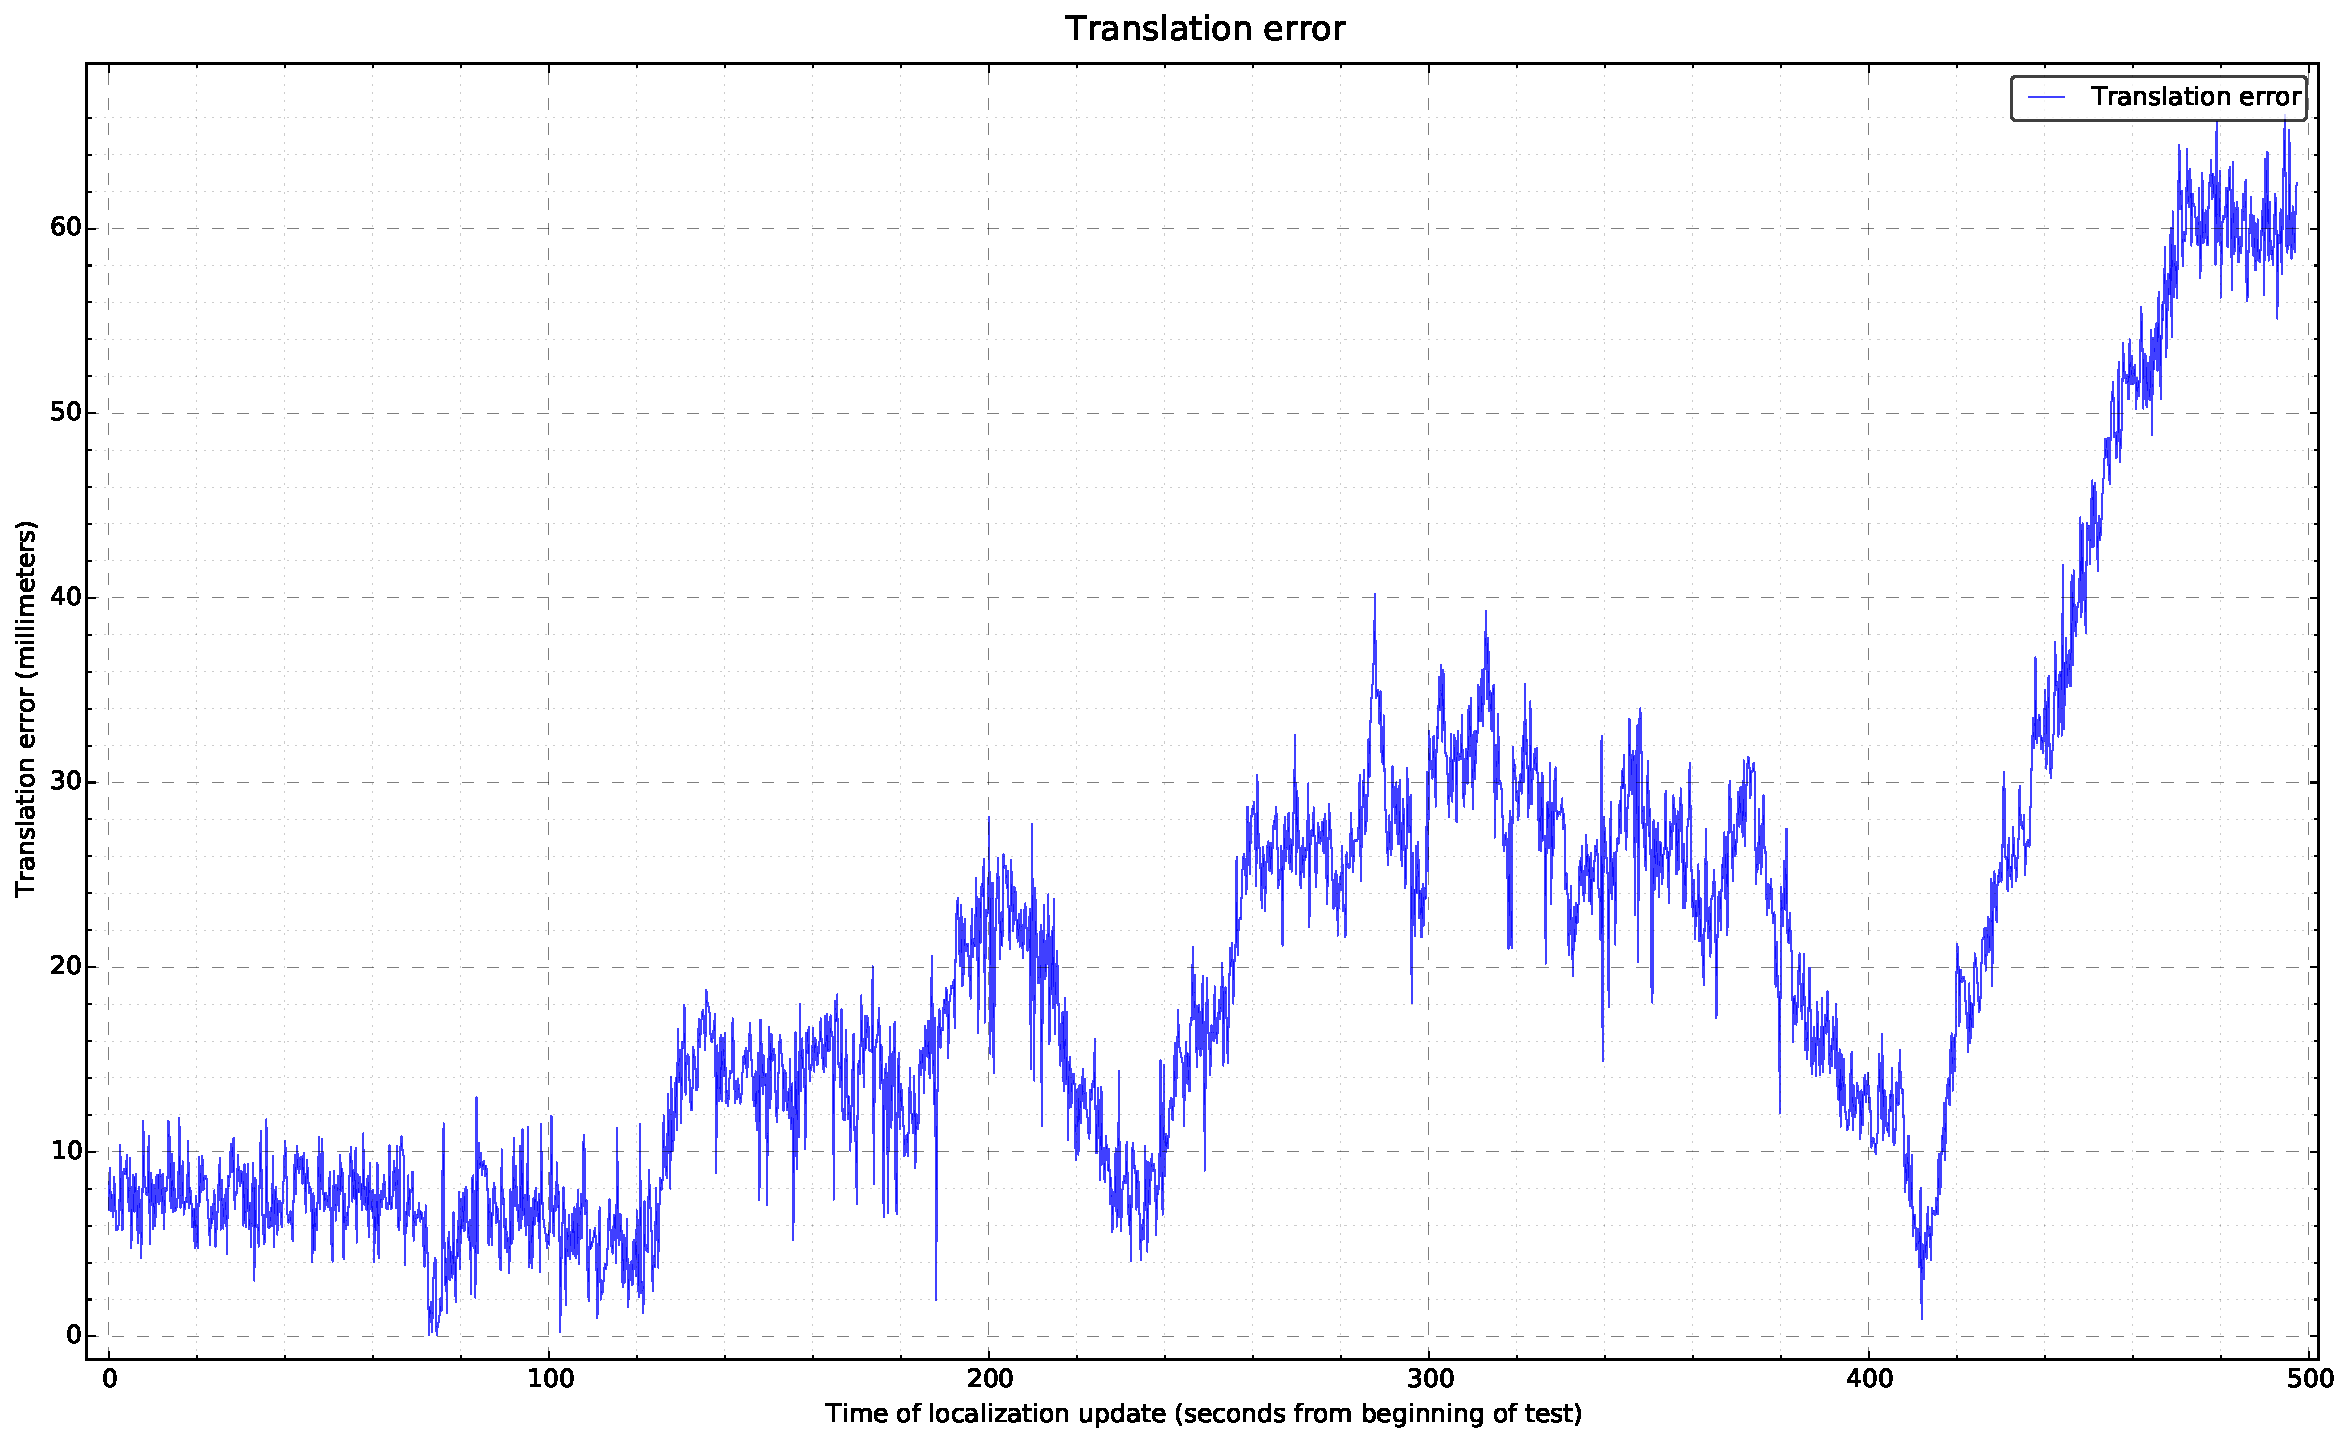
\includegraphics[width=0.69\textwidth]{appendices/tests-3dof/jarvis-robot/\currfilebase/graphs/odometry-translation-error-millimeters}
	\caption{Odometry translation errors}
\end{figure}

\begin{figure}[H]
	\centering
	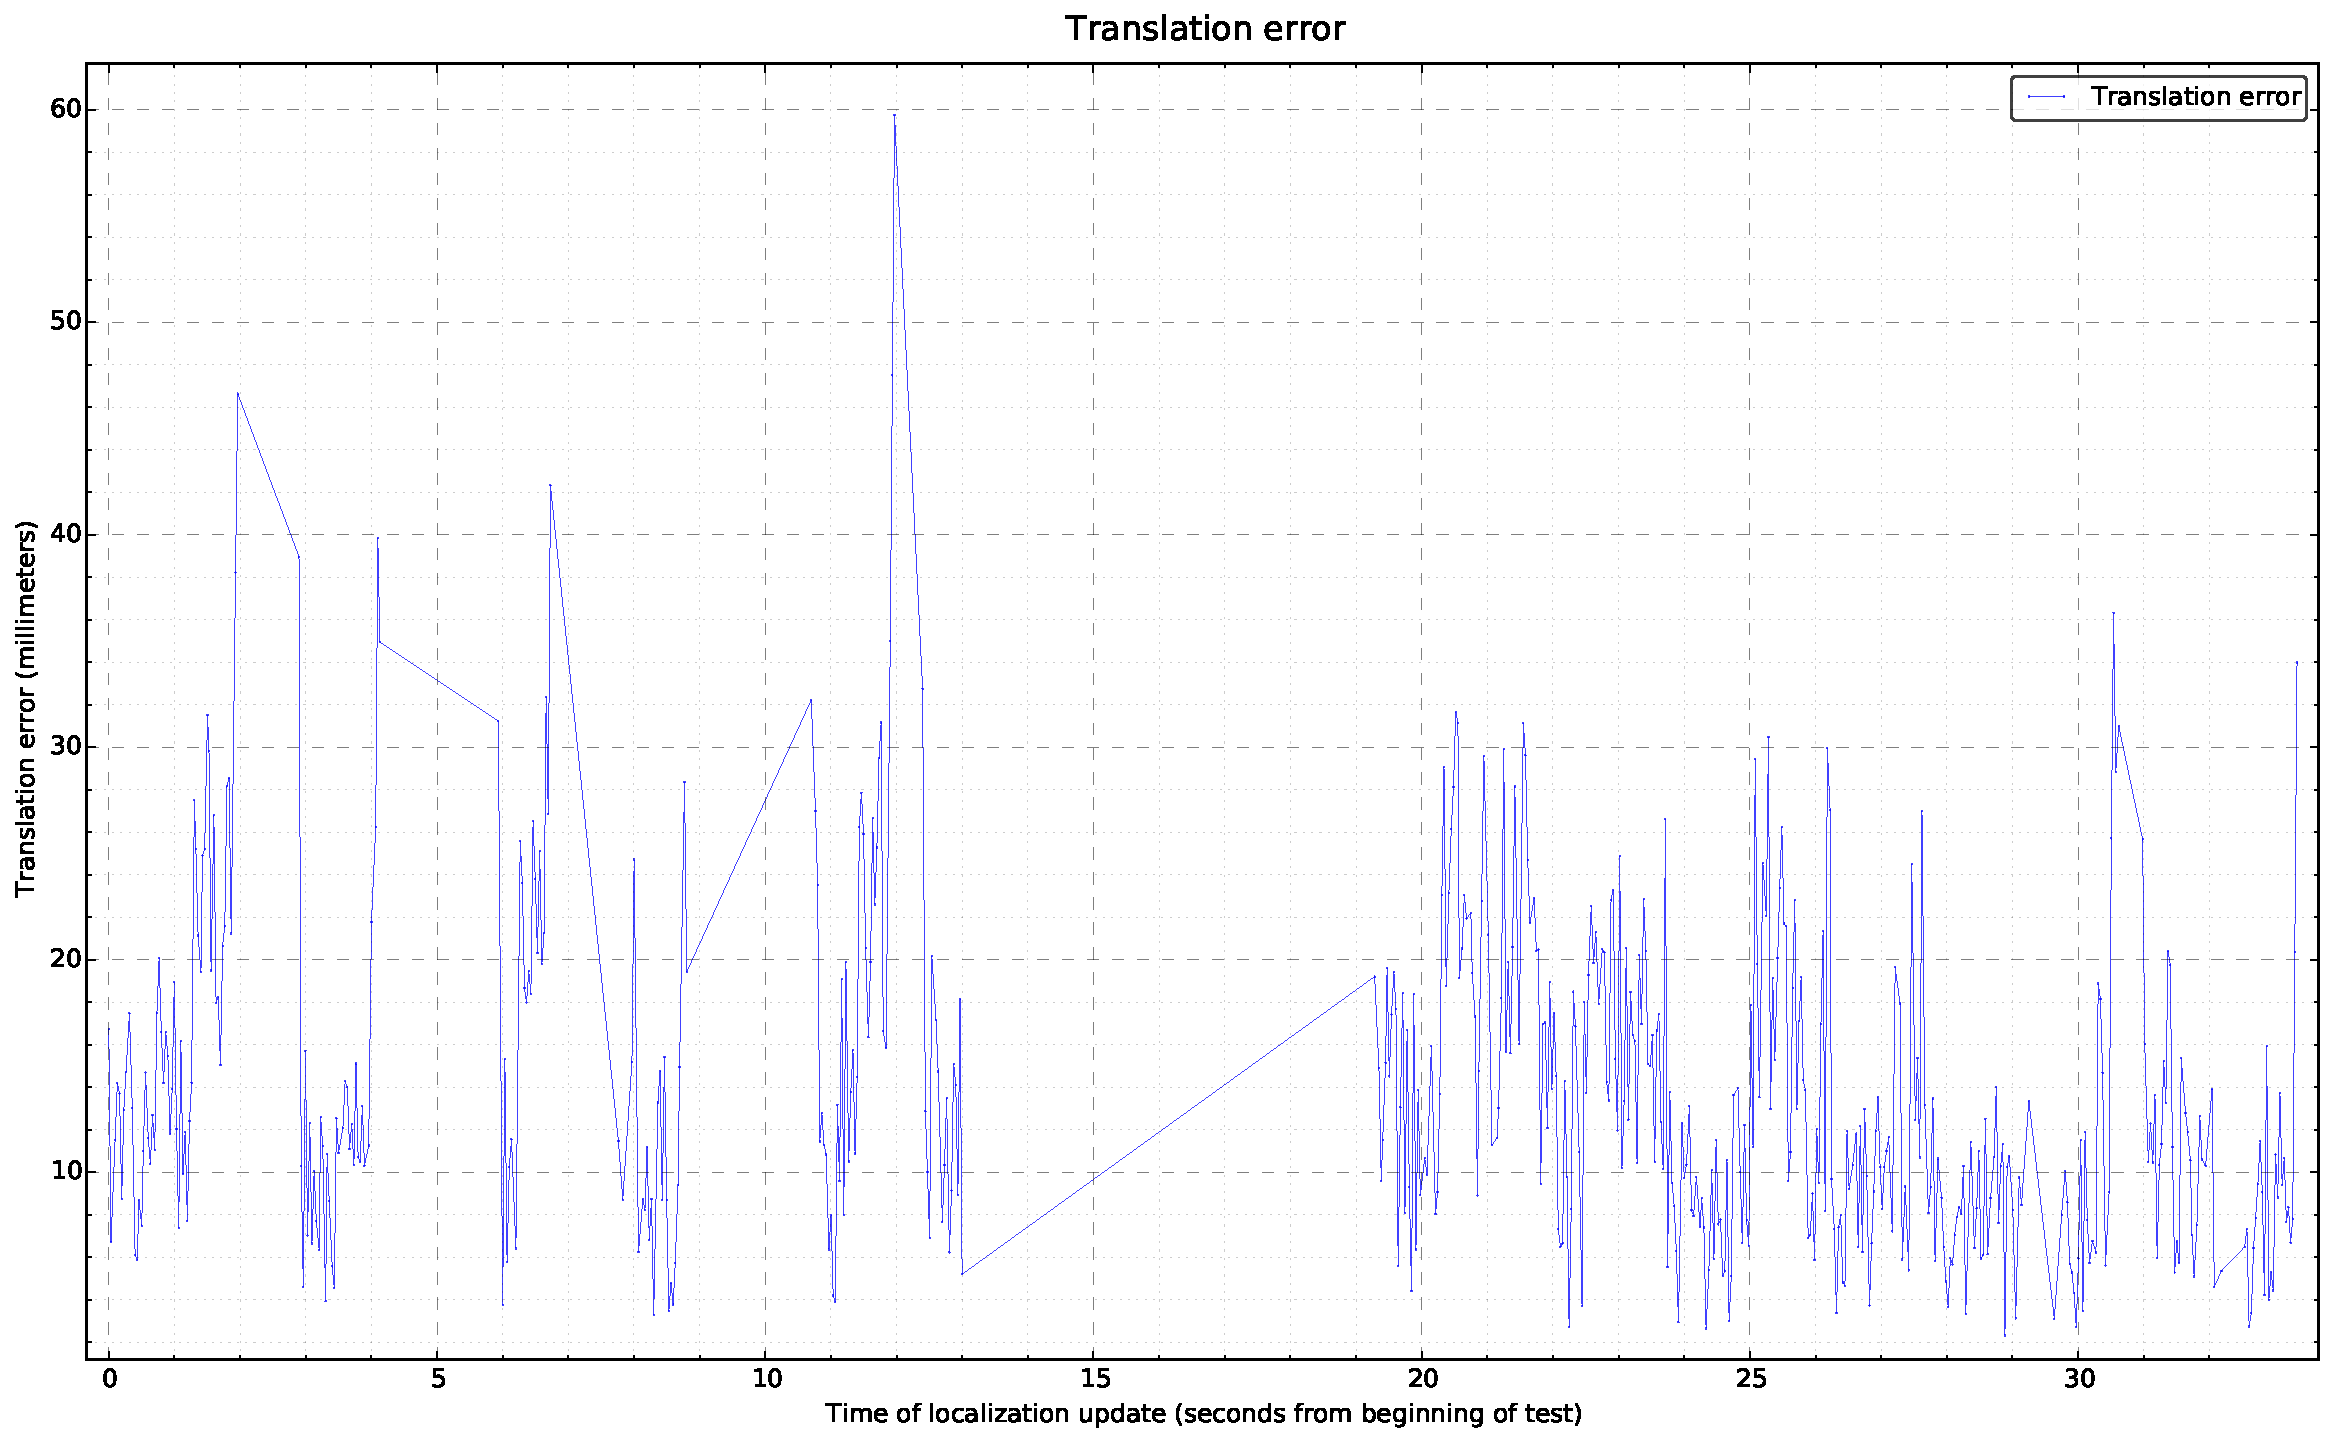
\includegraphics[width=0.69\textwidth]{appendices/tests-3dof/jarvis-robot/\currfilebase/graphs/translation-error-millimeters}
	\caption{Localization system translation errors}
\end{figure}

\begin{figure}[H]
	\centering
	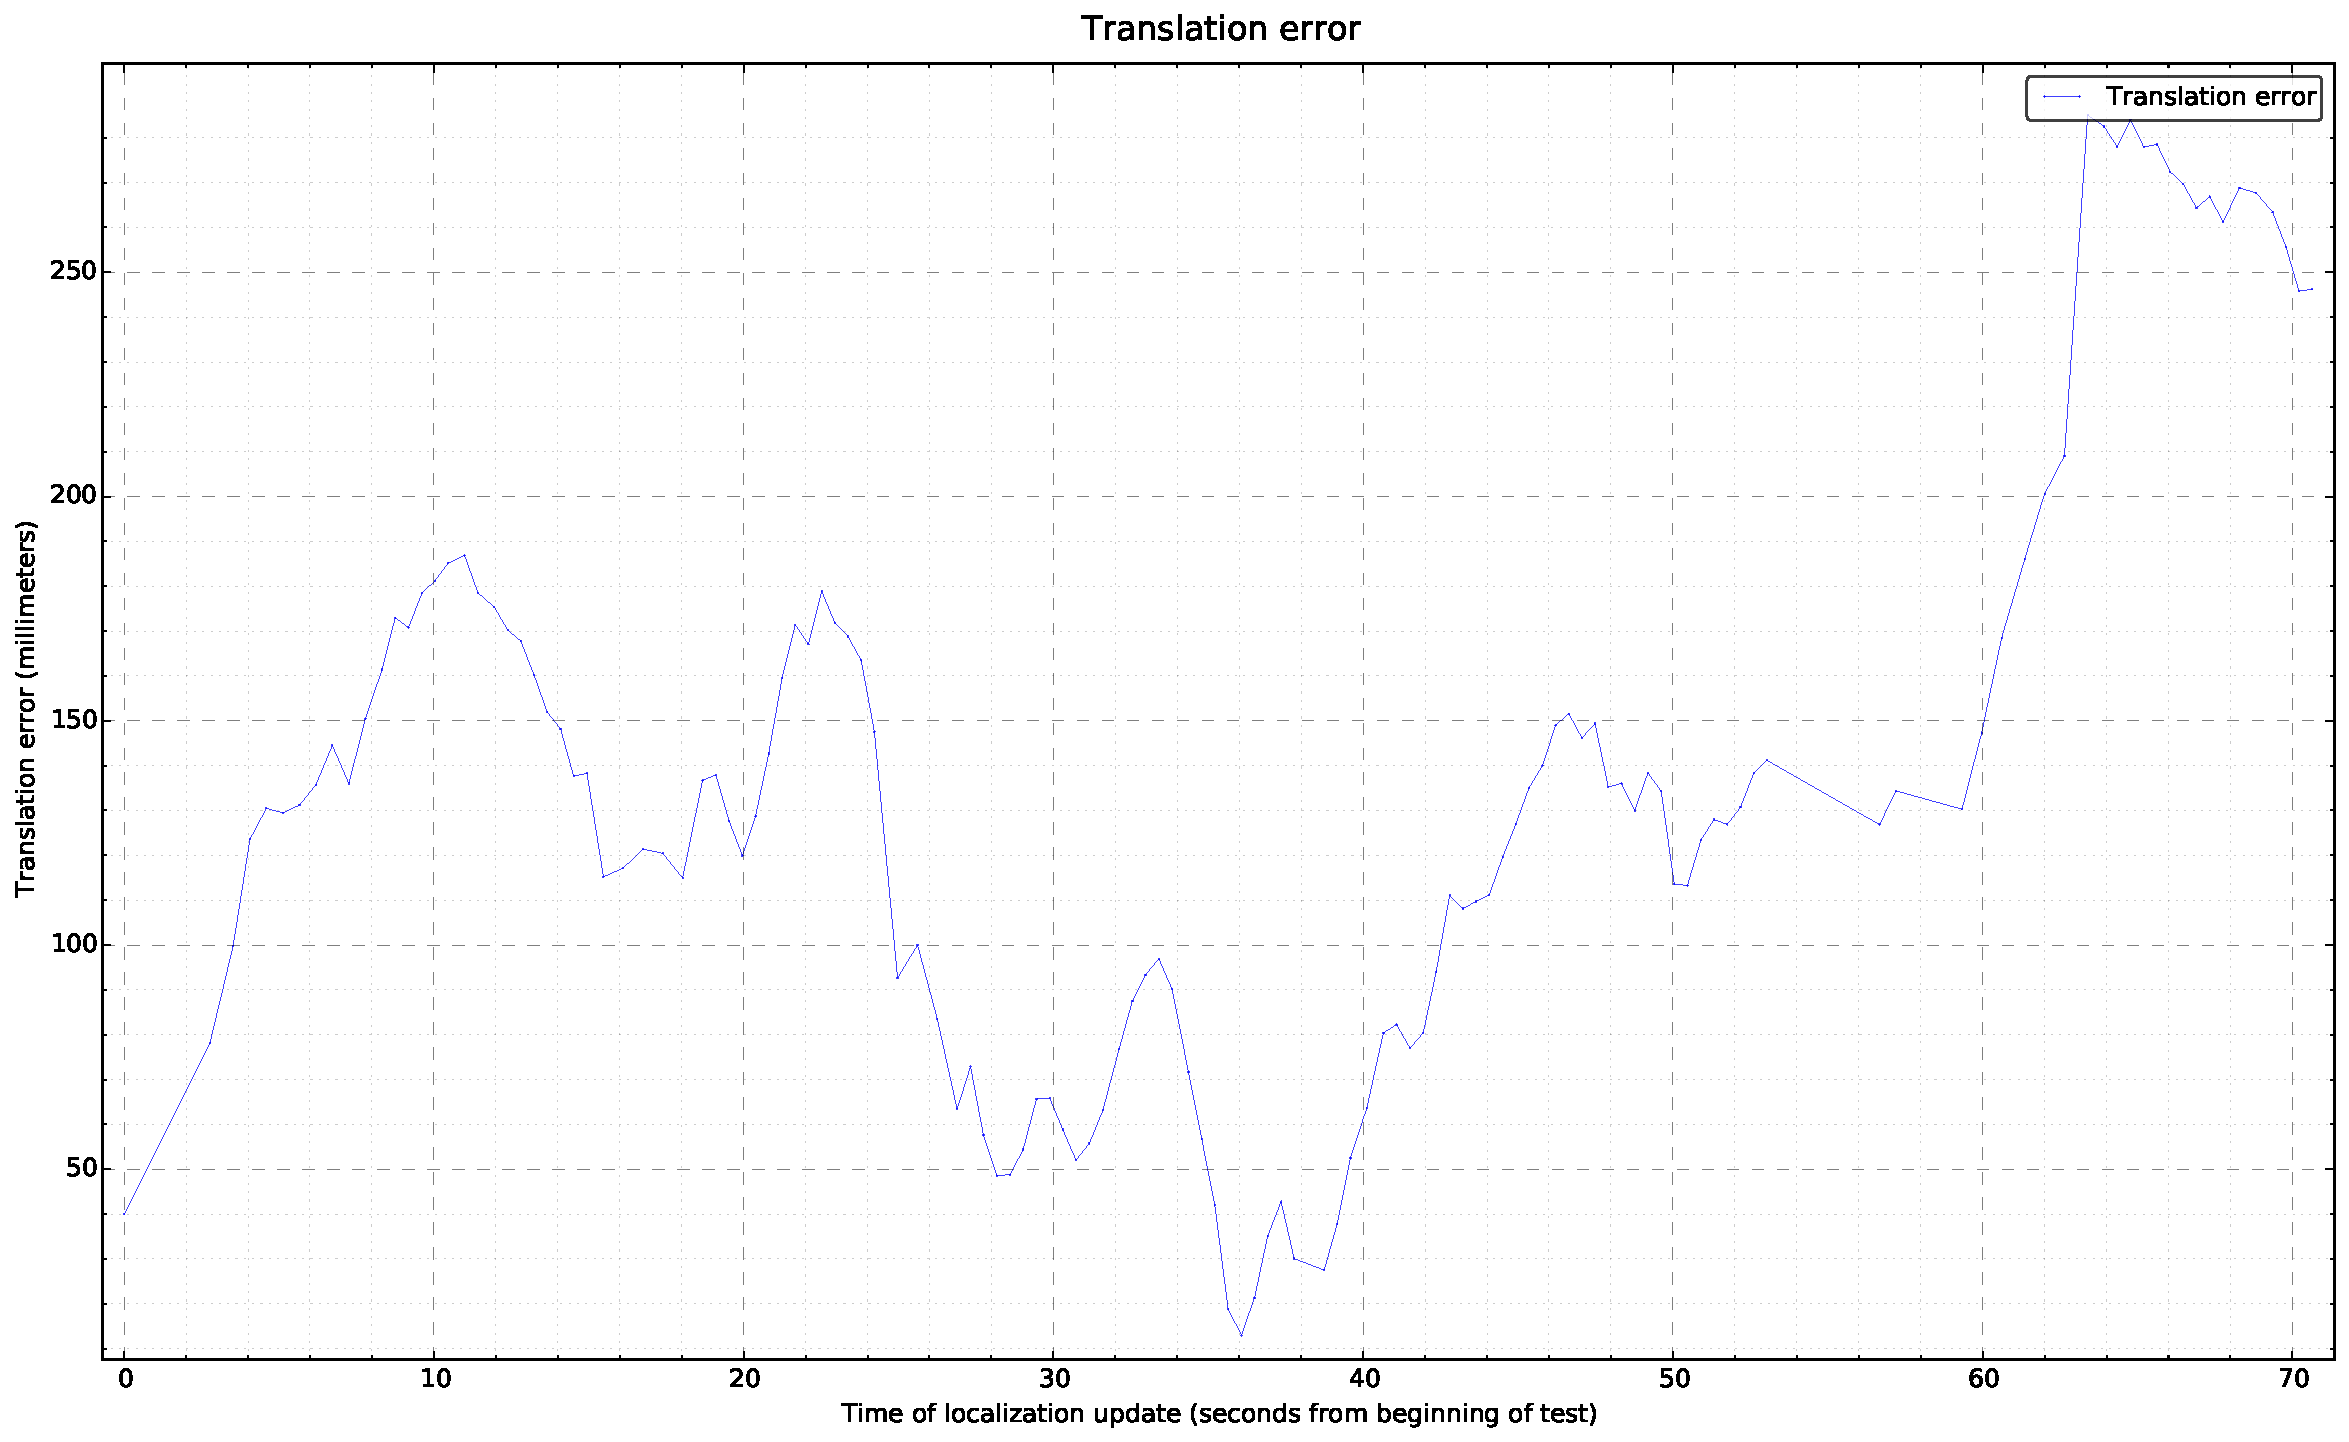
\includegraphics[width=0.69\textwidth]{appendices/tests-3dof/jarvis-robot/\currfilebase/graphs/translation-error-millimeters-amcl}
	\caption{\glsentrytext{amcl} translation errors}
\end{figure}


%Translation errors components
\begin{figure}[H]
	\centering
	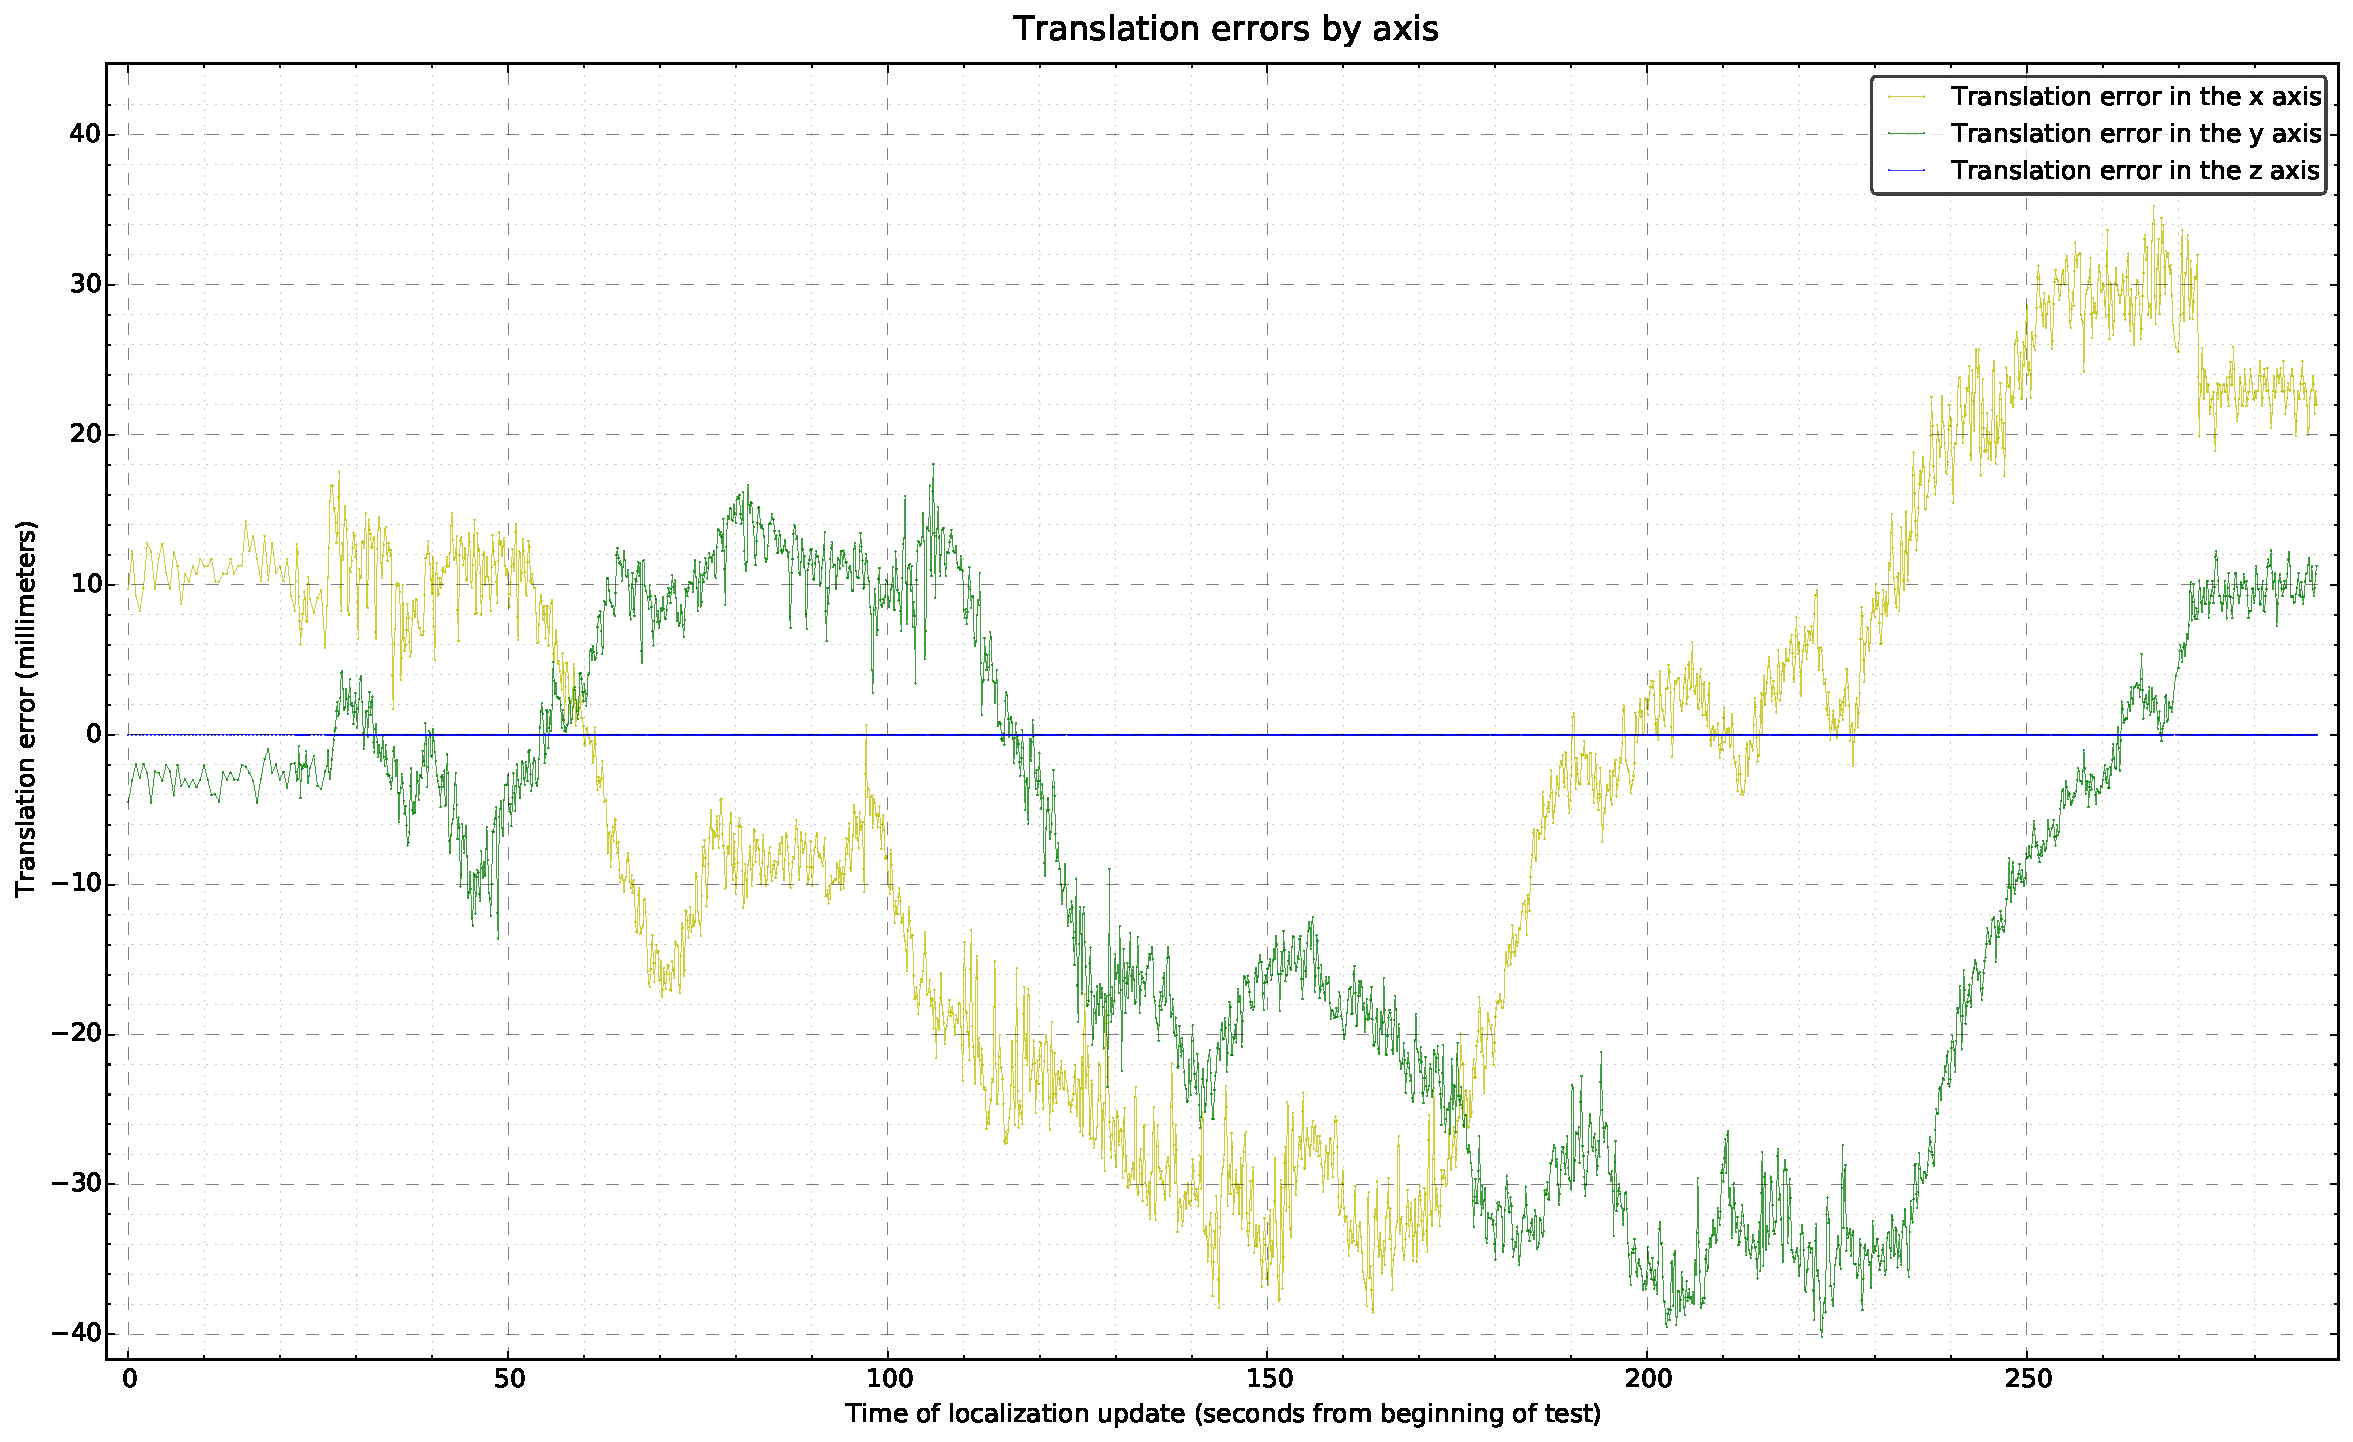
\includegraphics[width=0.69\textwidth]{appendices/tests-3dof/jarvis-robot/\currfilebase/graphs/odometry-translation-error-components-millimeters}
	\caption{Odometry translation errors components}
\end{figure}

\begin{figure}[H]
	\centering
	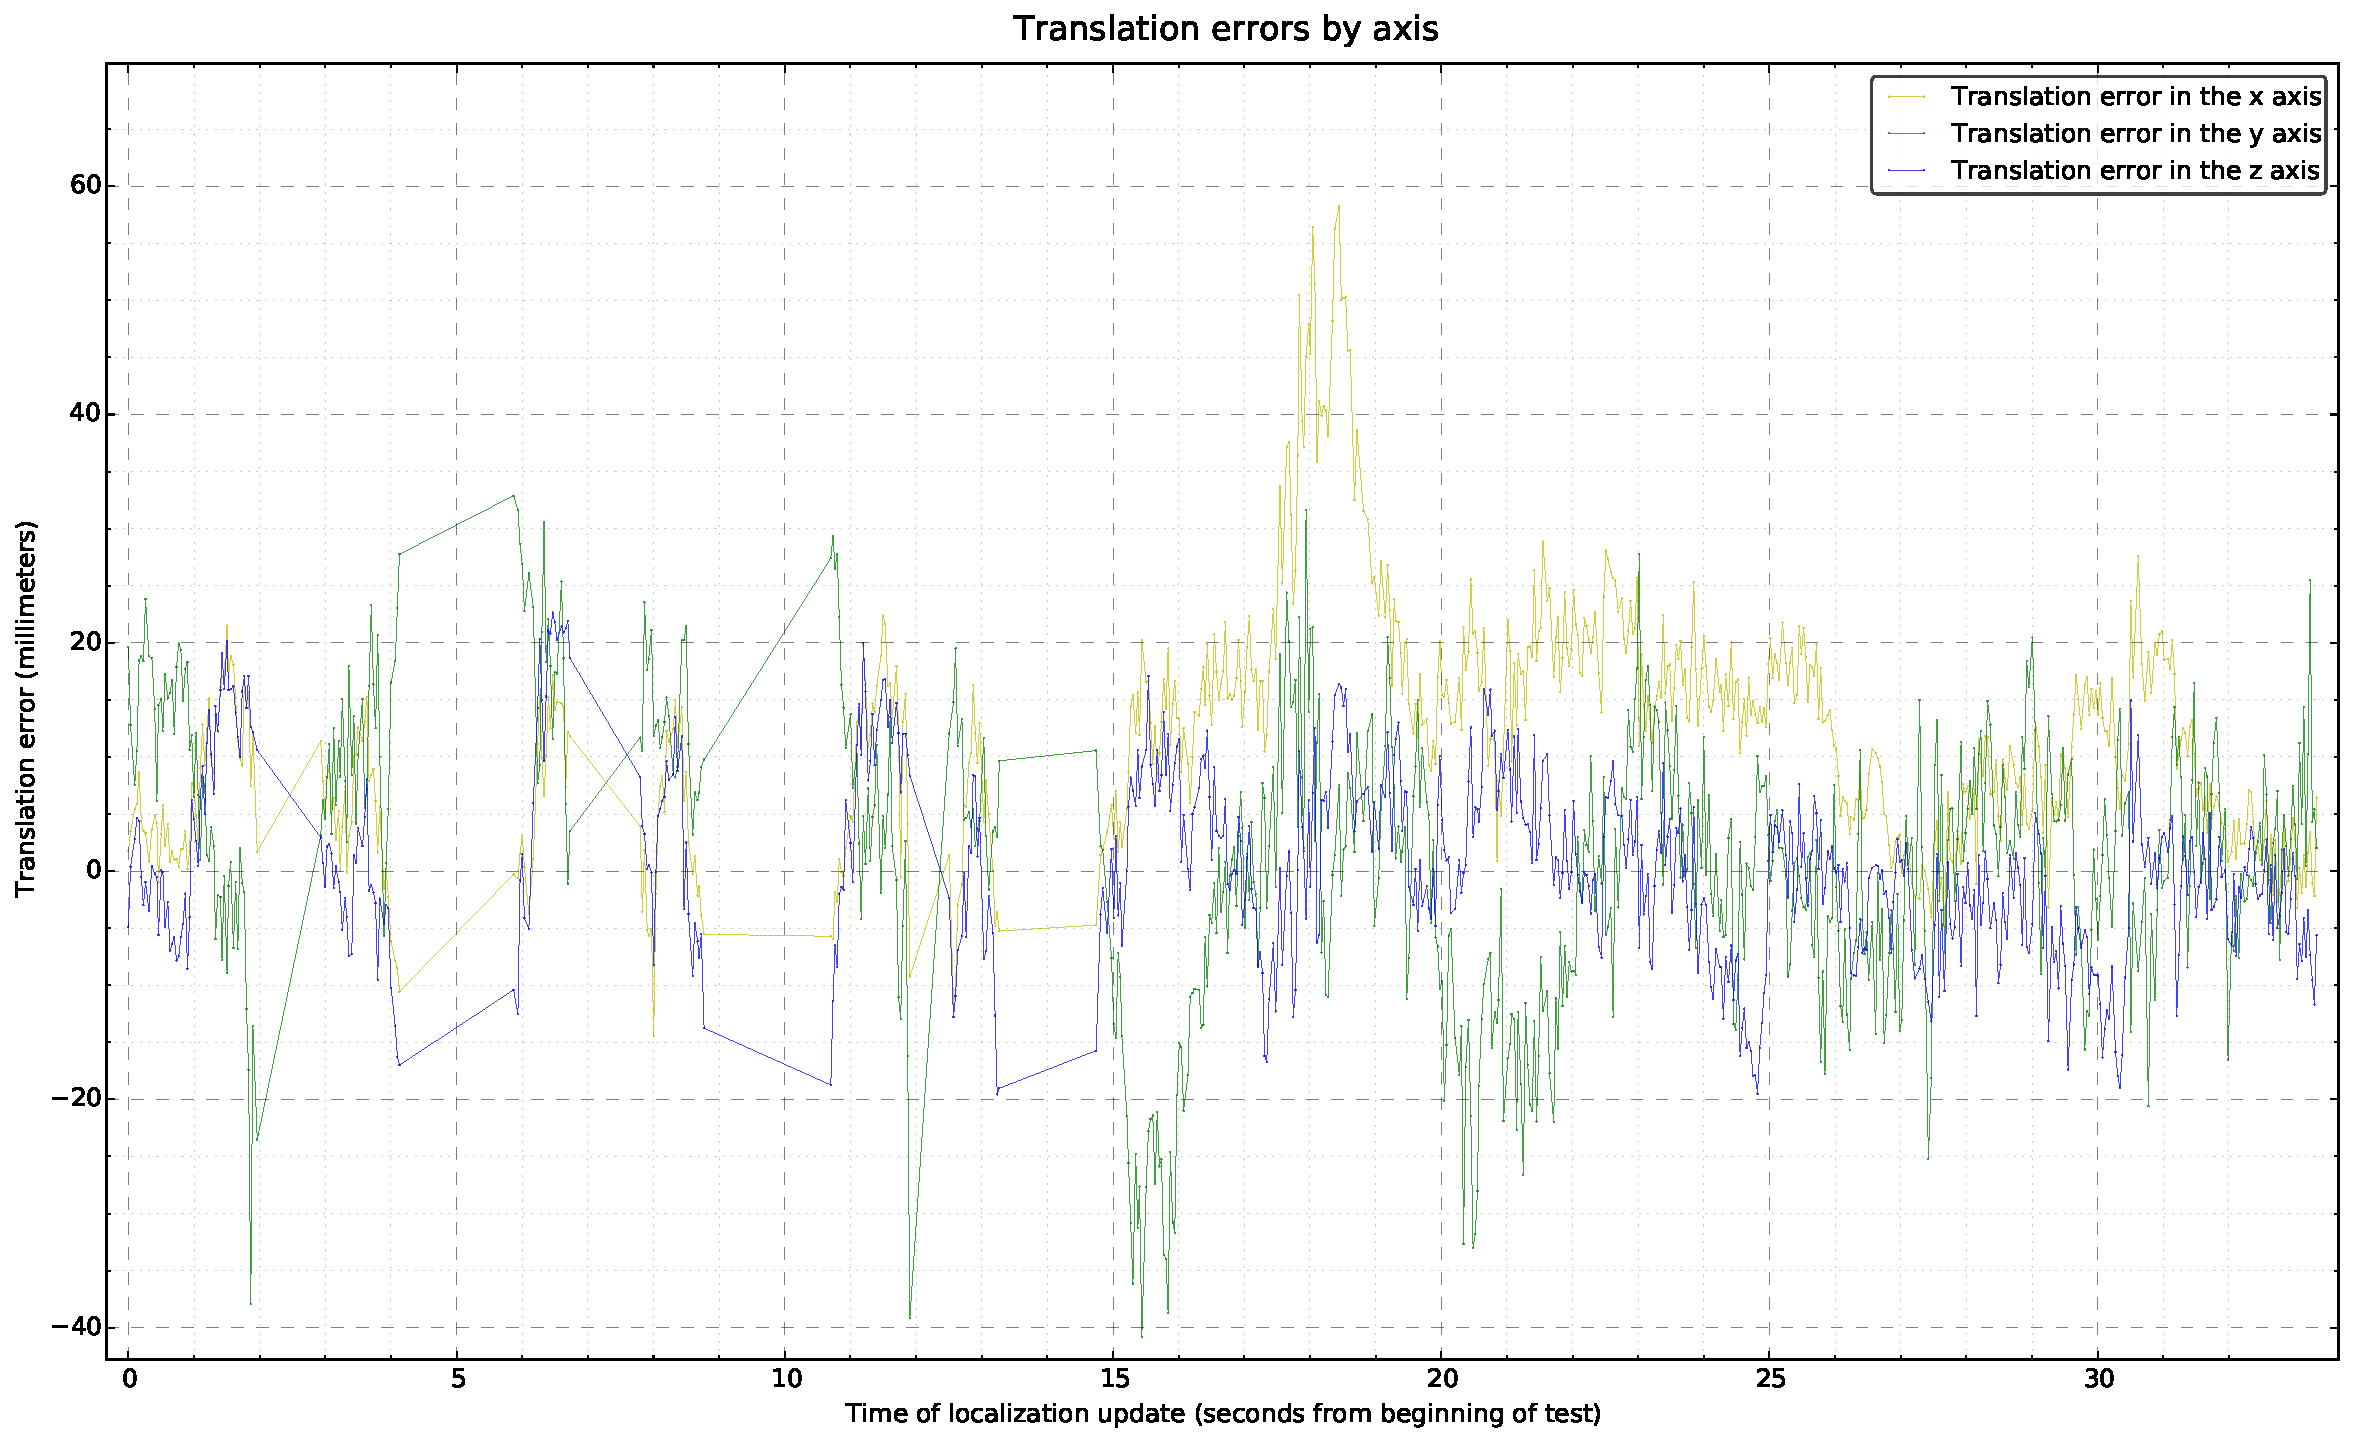
\includegraphics[width=0.69\textwidth]{appendices/tests-3dof/jarvis-robot/\currfilebase/graphs/translation-error-components-millimeters}
	\caption{Localization system translation errors components}
\end{figure}

\begin{figure}[H]
	\centering
	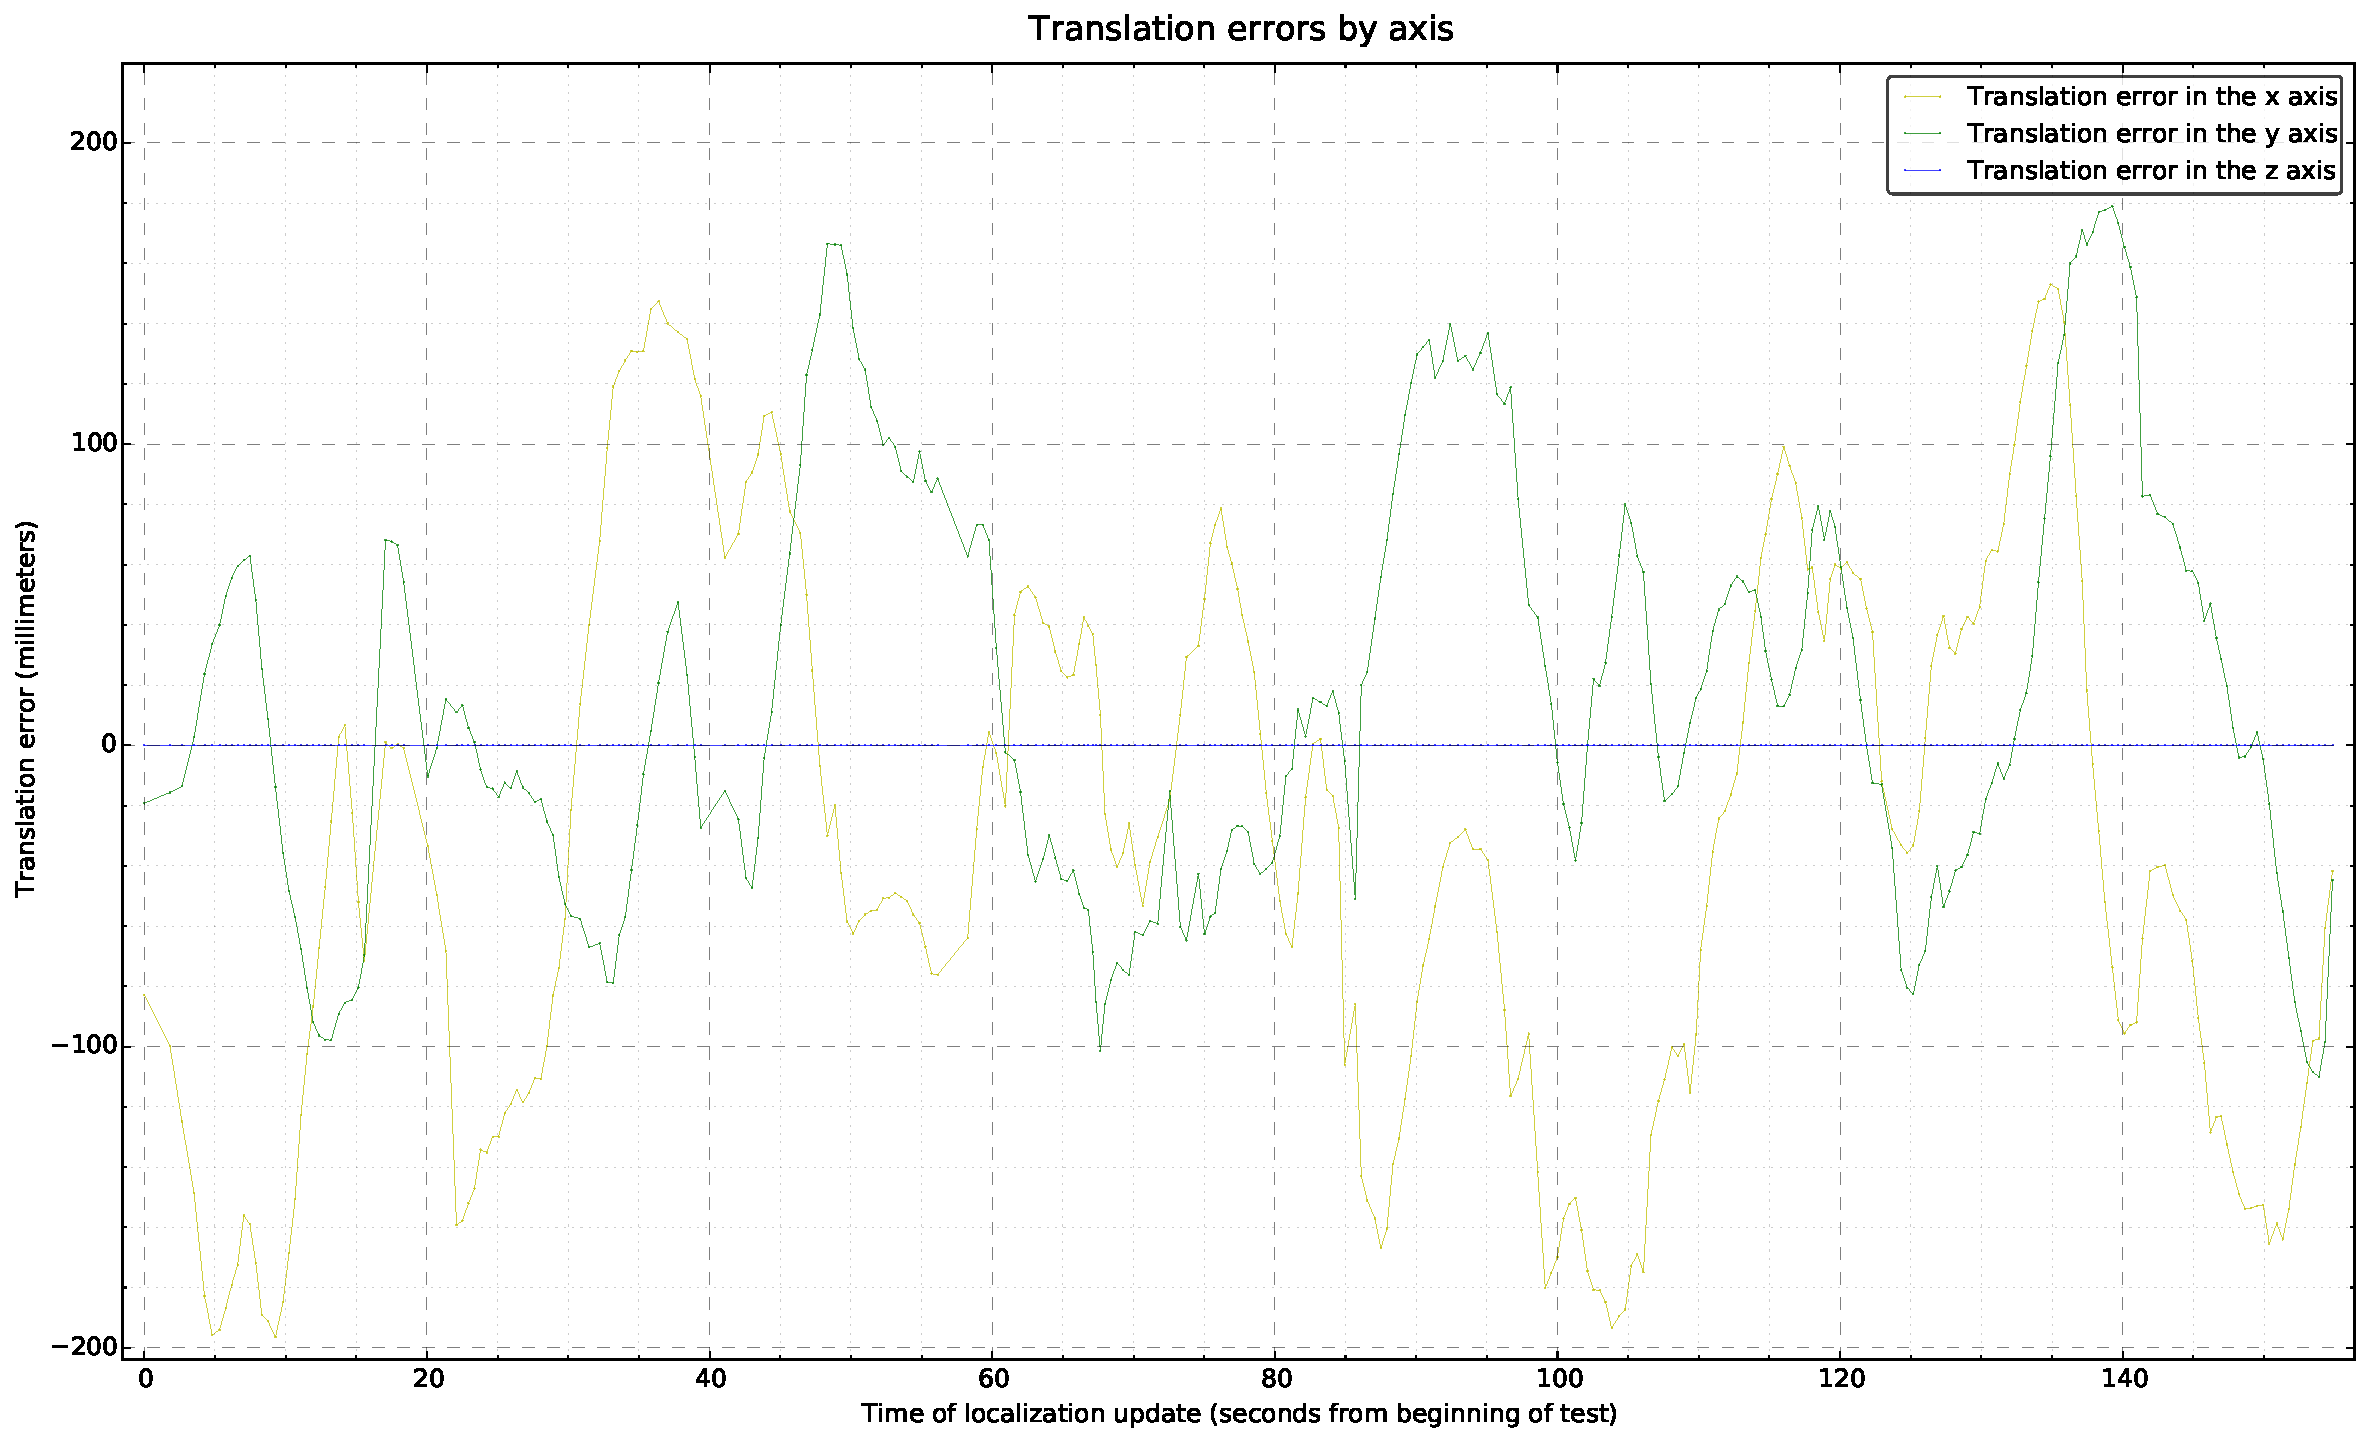
\includegraphics[width=0.69\textwidth]{appendices/tests-3dof/jarvis-robot/\currfilebase/graphs/translation-error-components-millimeters-amcl}
	\caption{\glsentrytext{amcl} translation errors components}
\end{figure}


%Translation errors distributions
\begin{figure}[H]
	\centering
	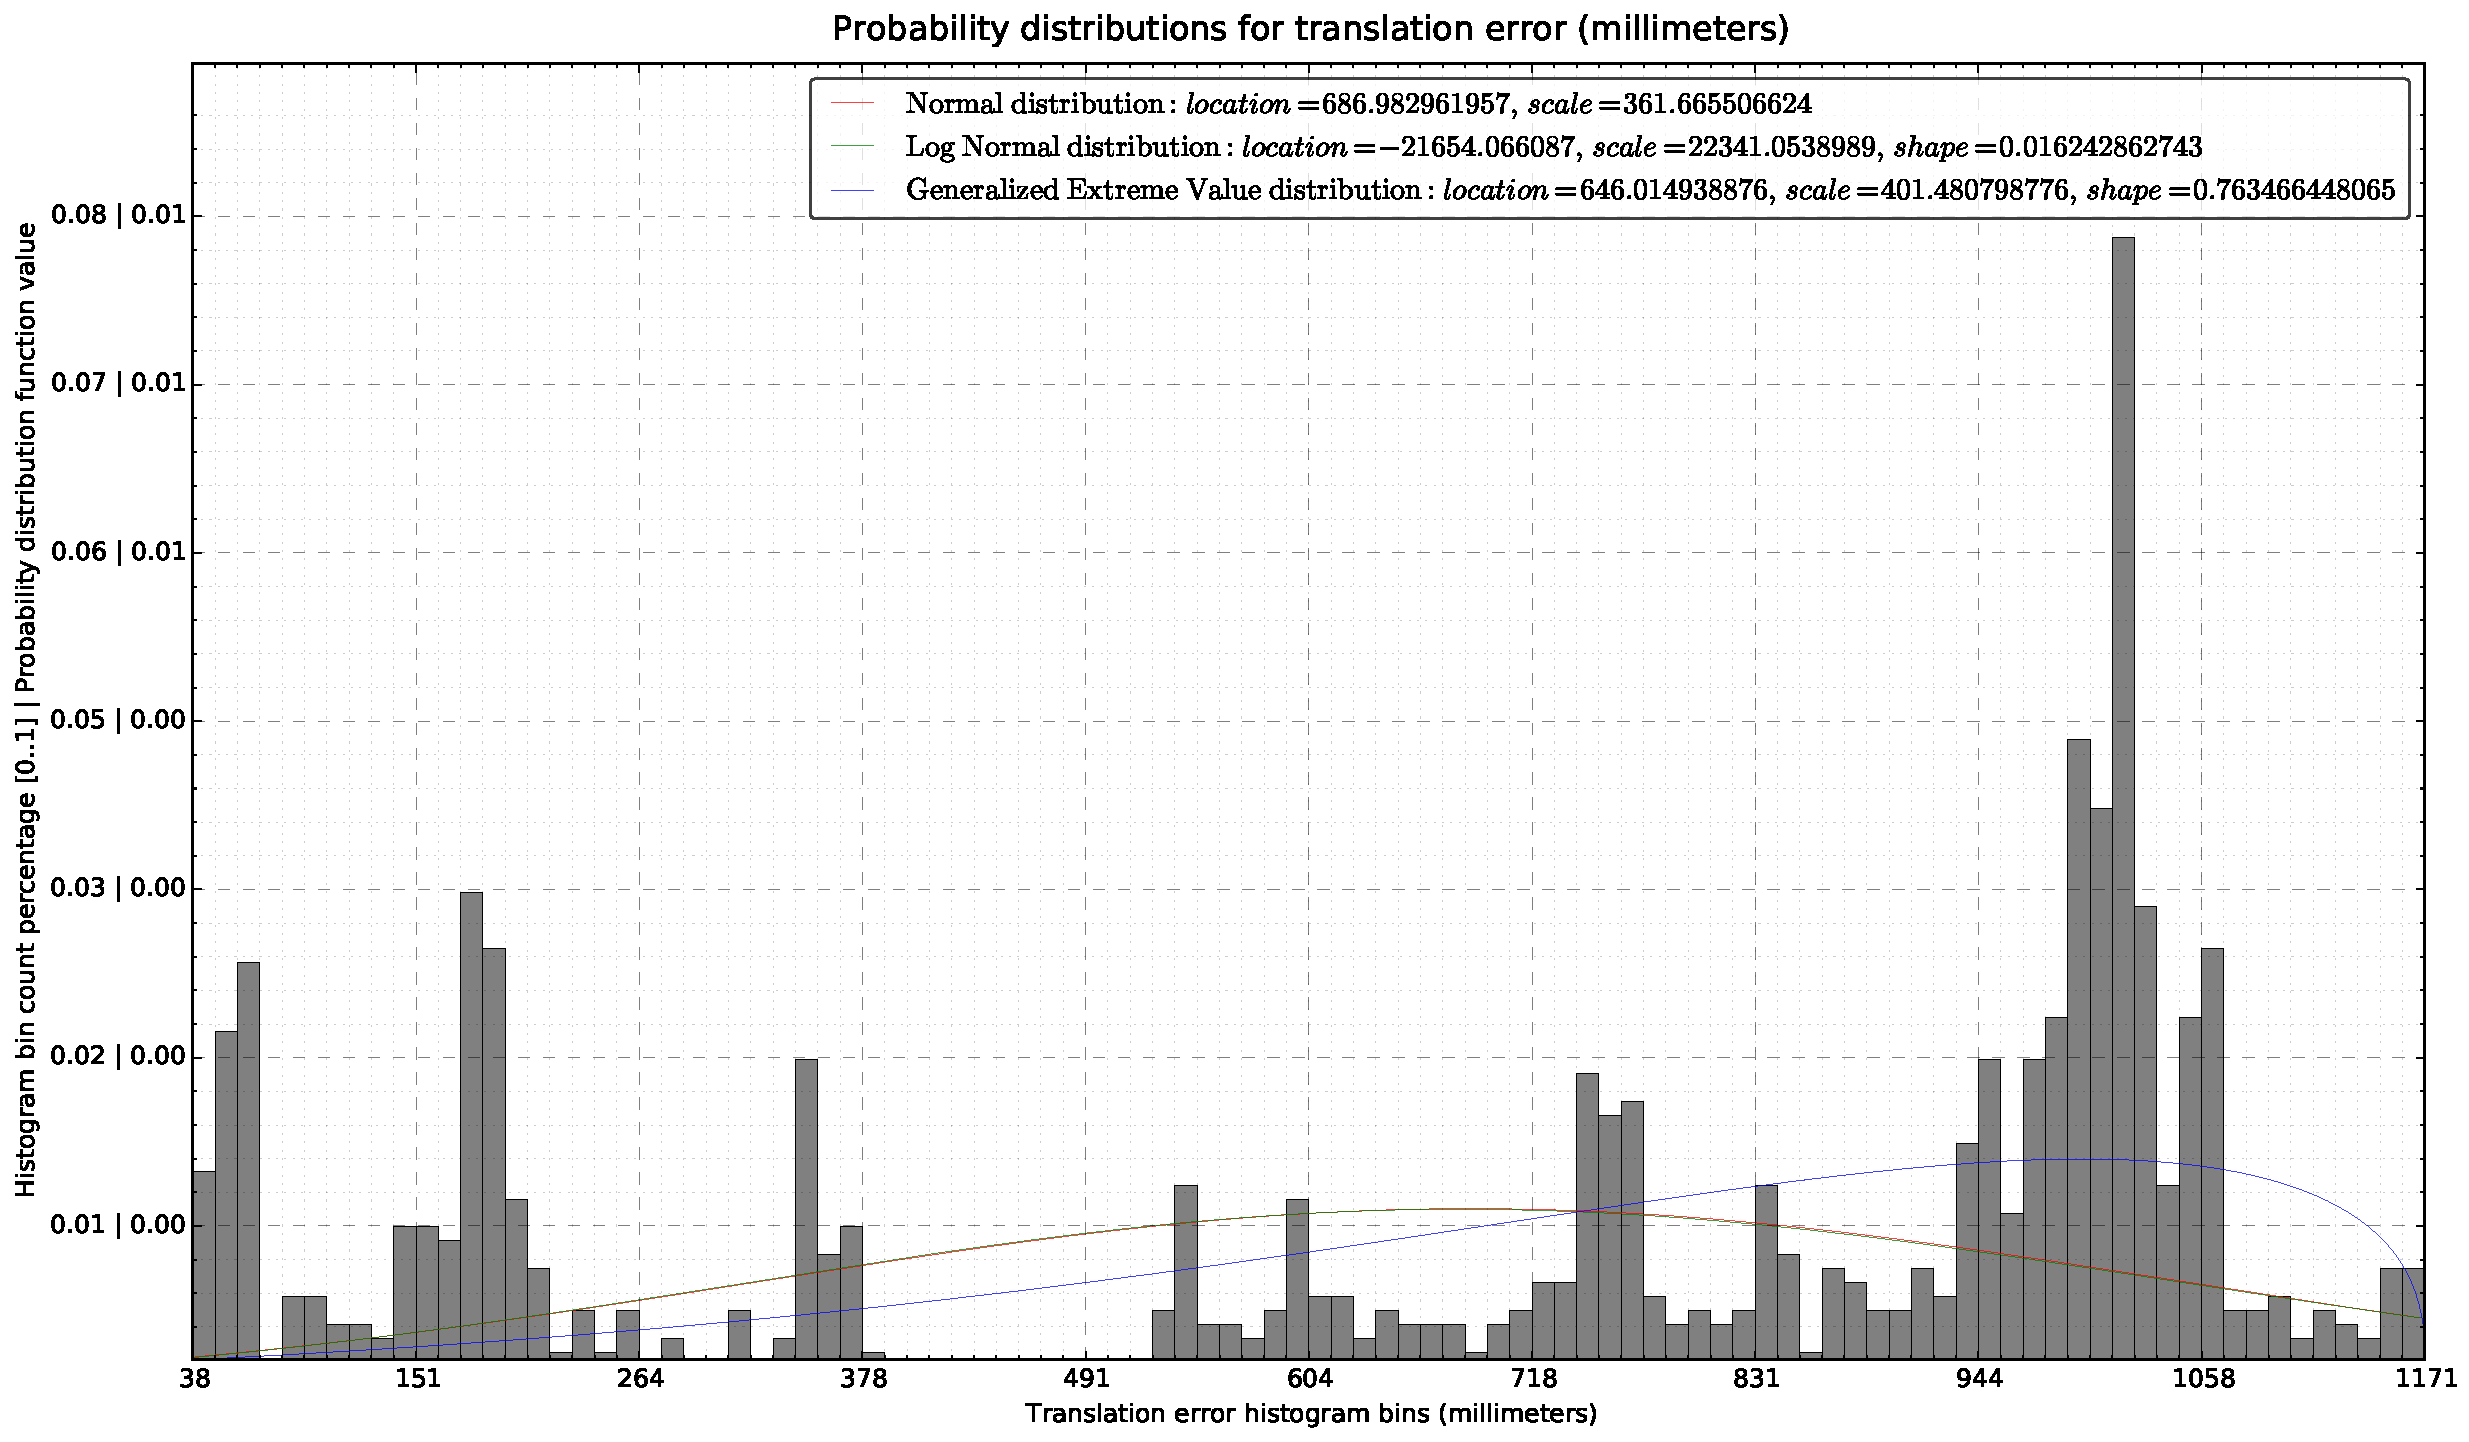
\includegraphics[width=0.73\textwidth]{appendices/tests-3dof/jarvis-robot/\currfilebase/graphs/odometry-translation-error-millimeters-distributions}
	\caption{Probability distributions for the odometry translation errors}
\end{figure}

\begin{figure}[H]
	\centering
	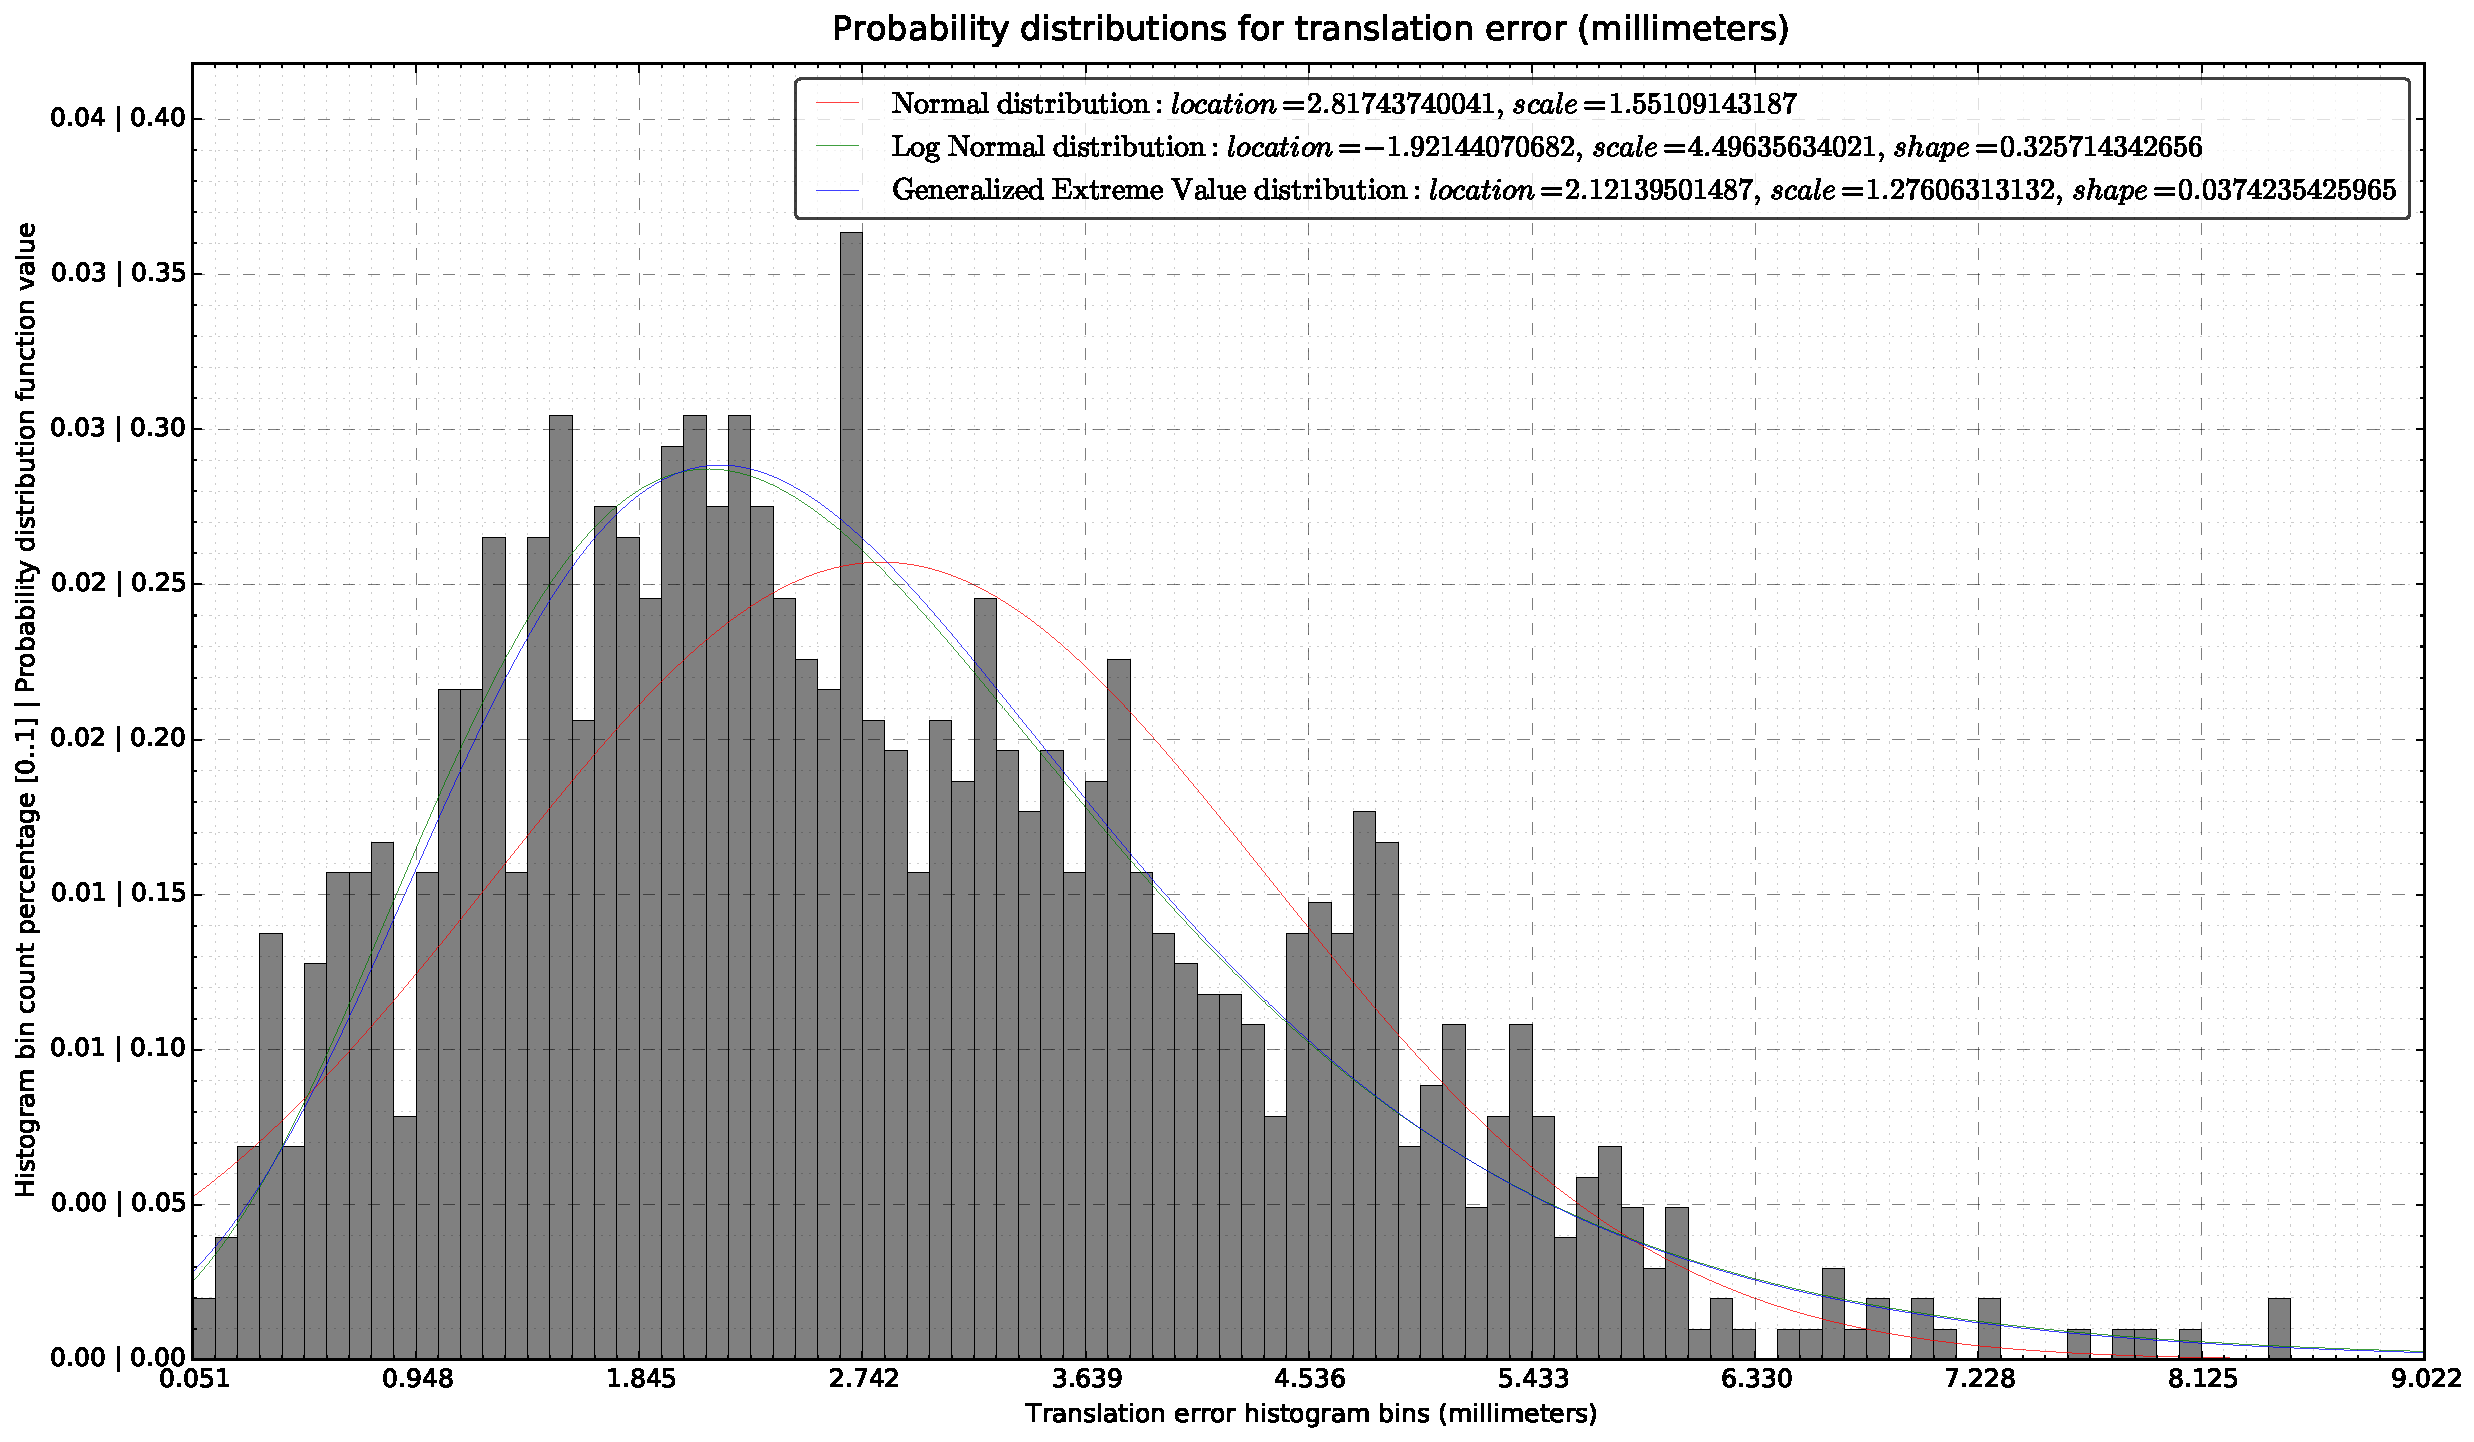
\includegraphics[width=0.73\textwidth]{appendices/tests-3dof/jarvis-robot/\currfilebase/graphs/translation-error-millimeters-distributions}
	\caption{Probability distributions for the localization system translation errors}
\end{figure}

\begin{figure}[H]
	\centering
	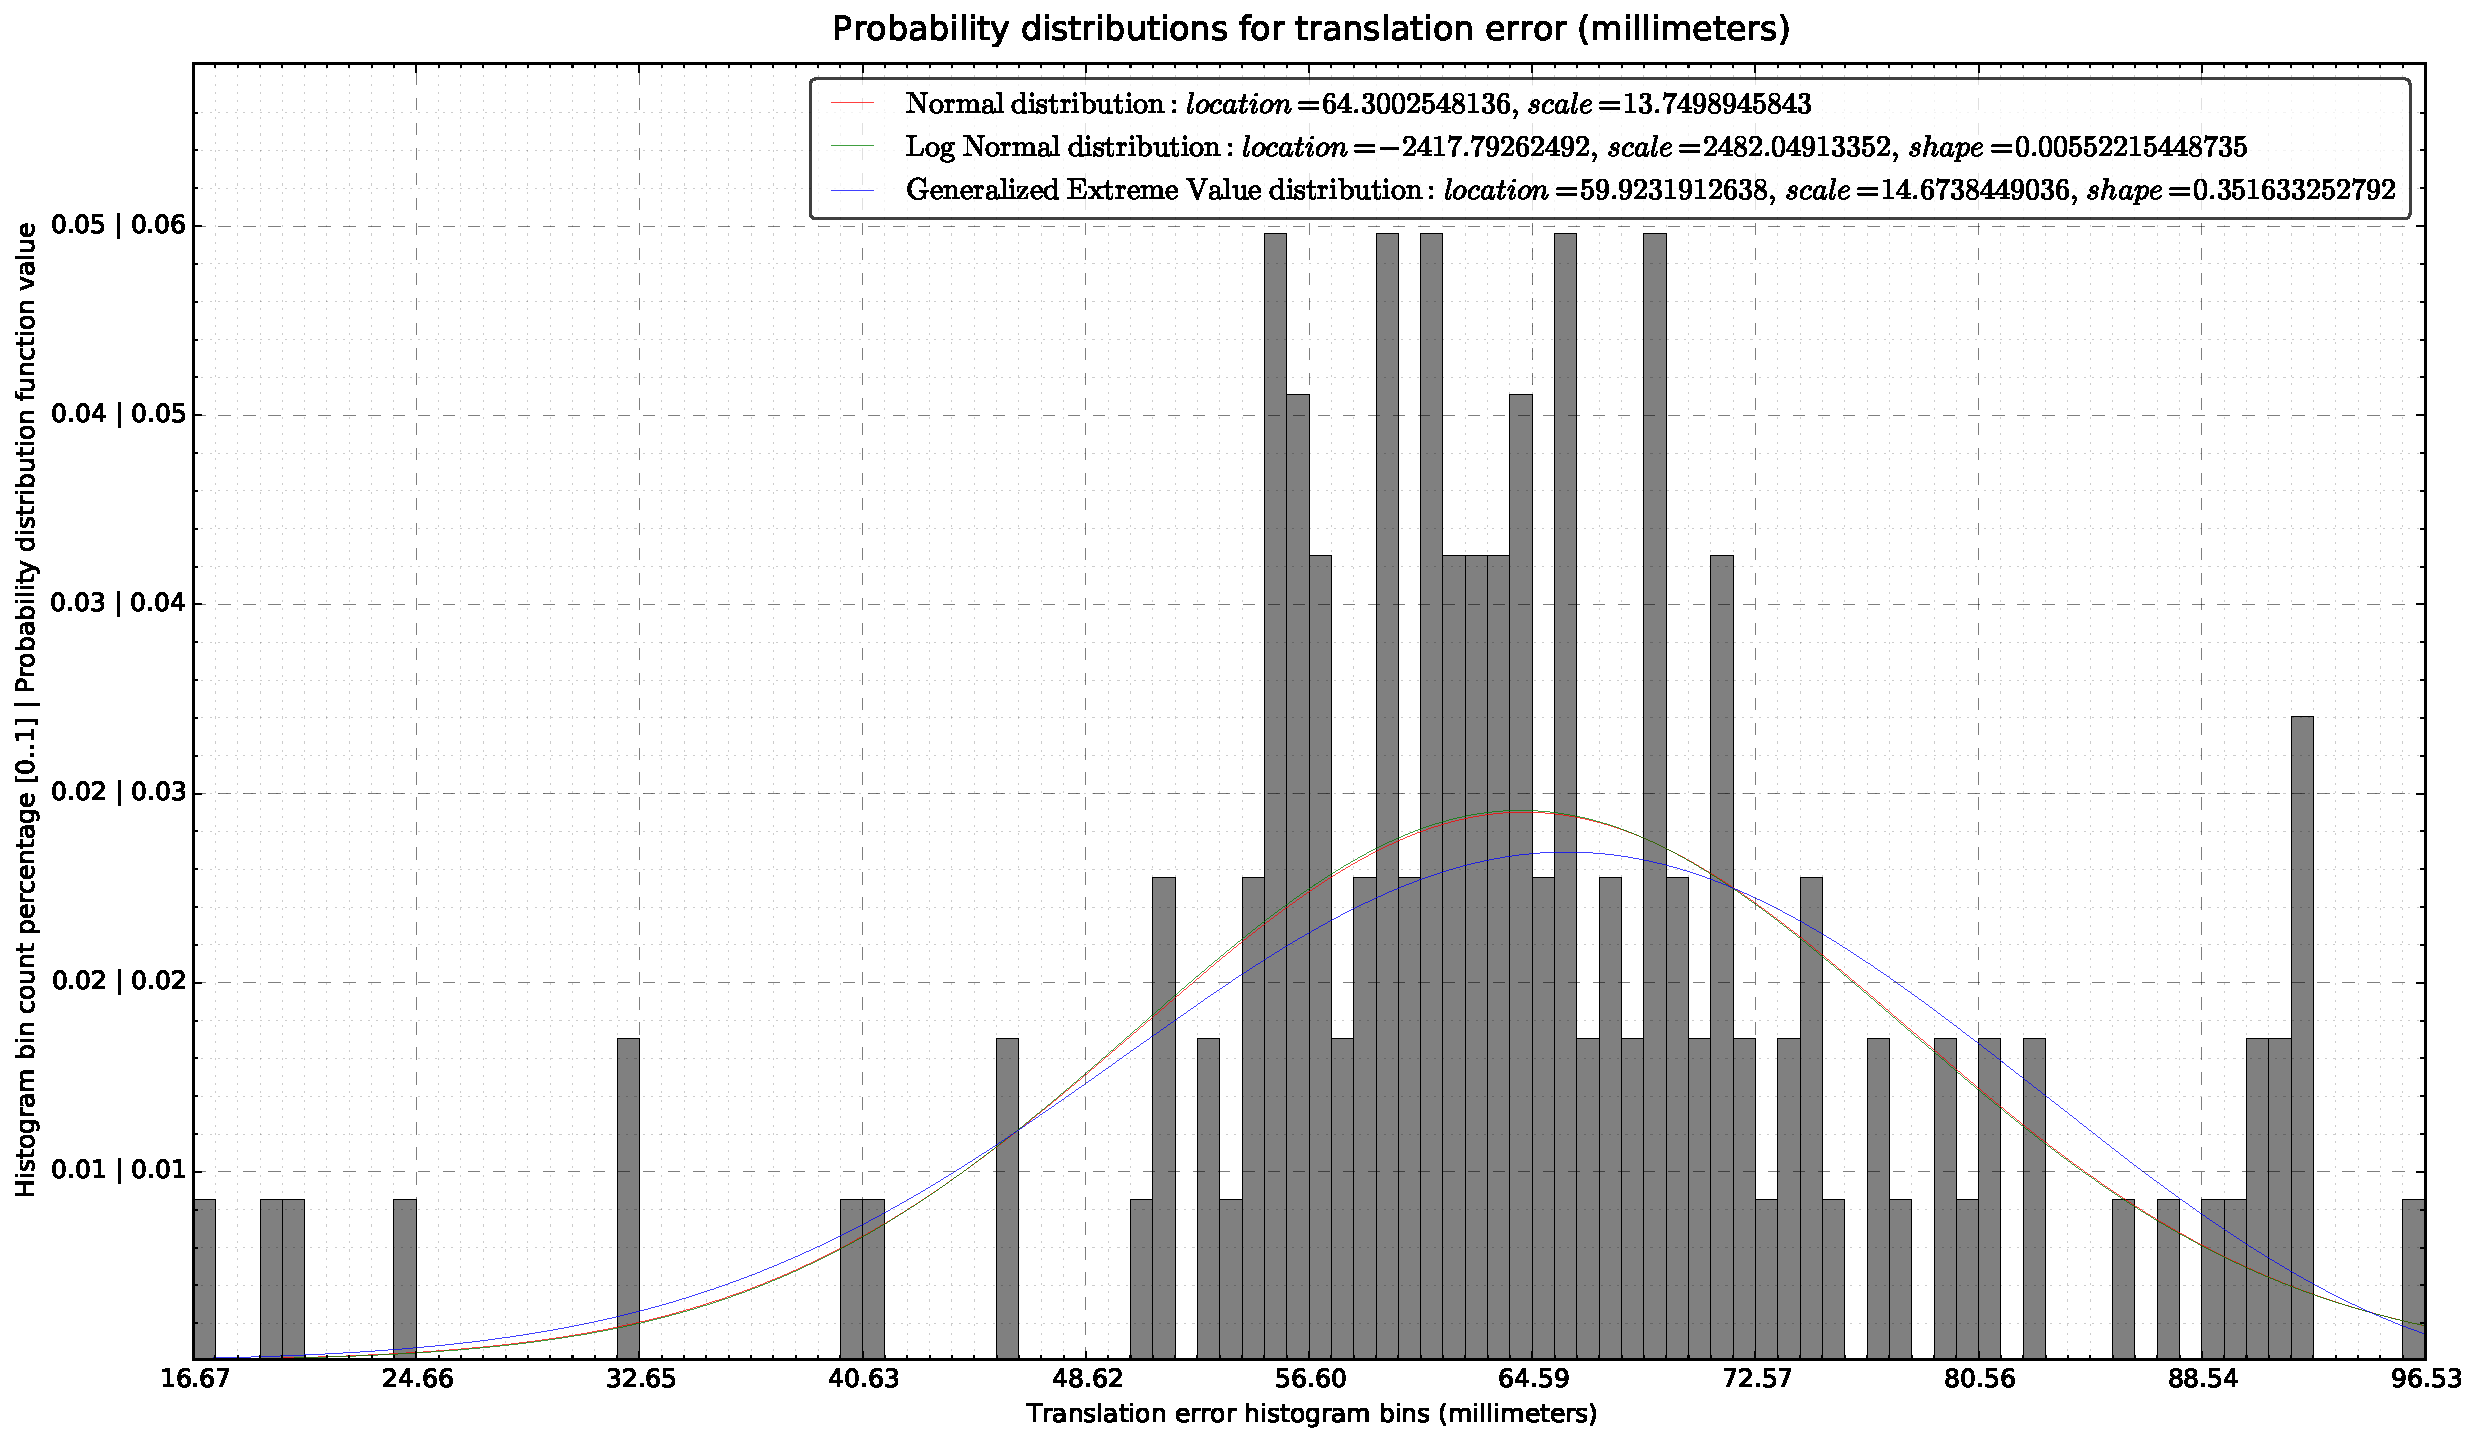
\includegraphics[width=0.73\textwidth]{appendices/tests-3dof/jarvis-robot/\currfilebase/graphs/translation-error-millimeters-distributions-amcl}
	\caption{Probability distributions for the \glsentrytext{amcl} translation errors}
\end{figure}


%Angular errors axis
\begin{figure}[H]
	\centering
	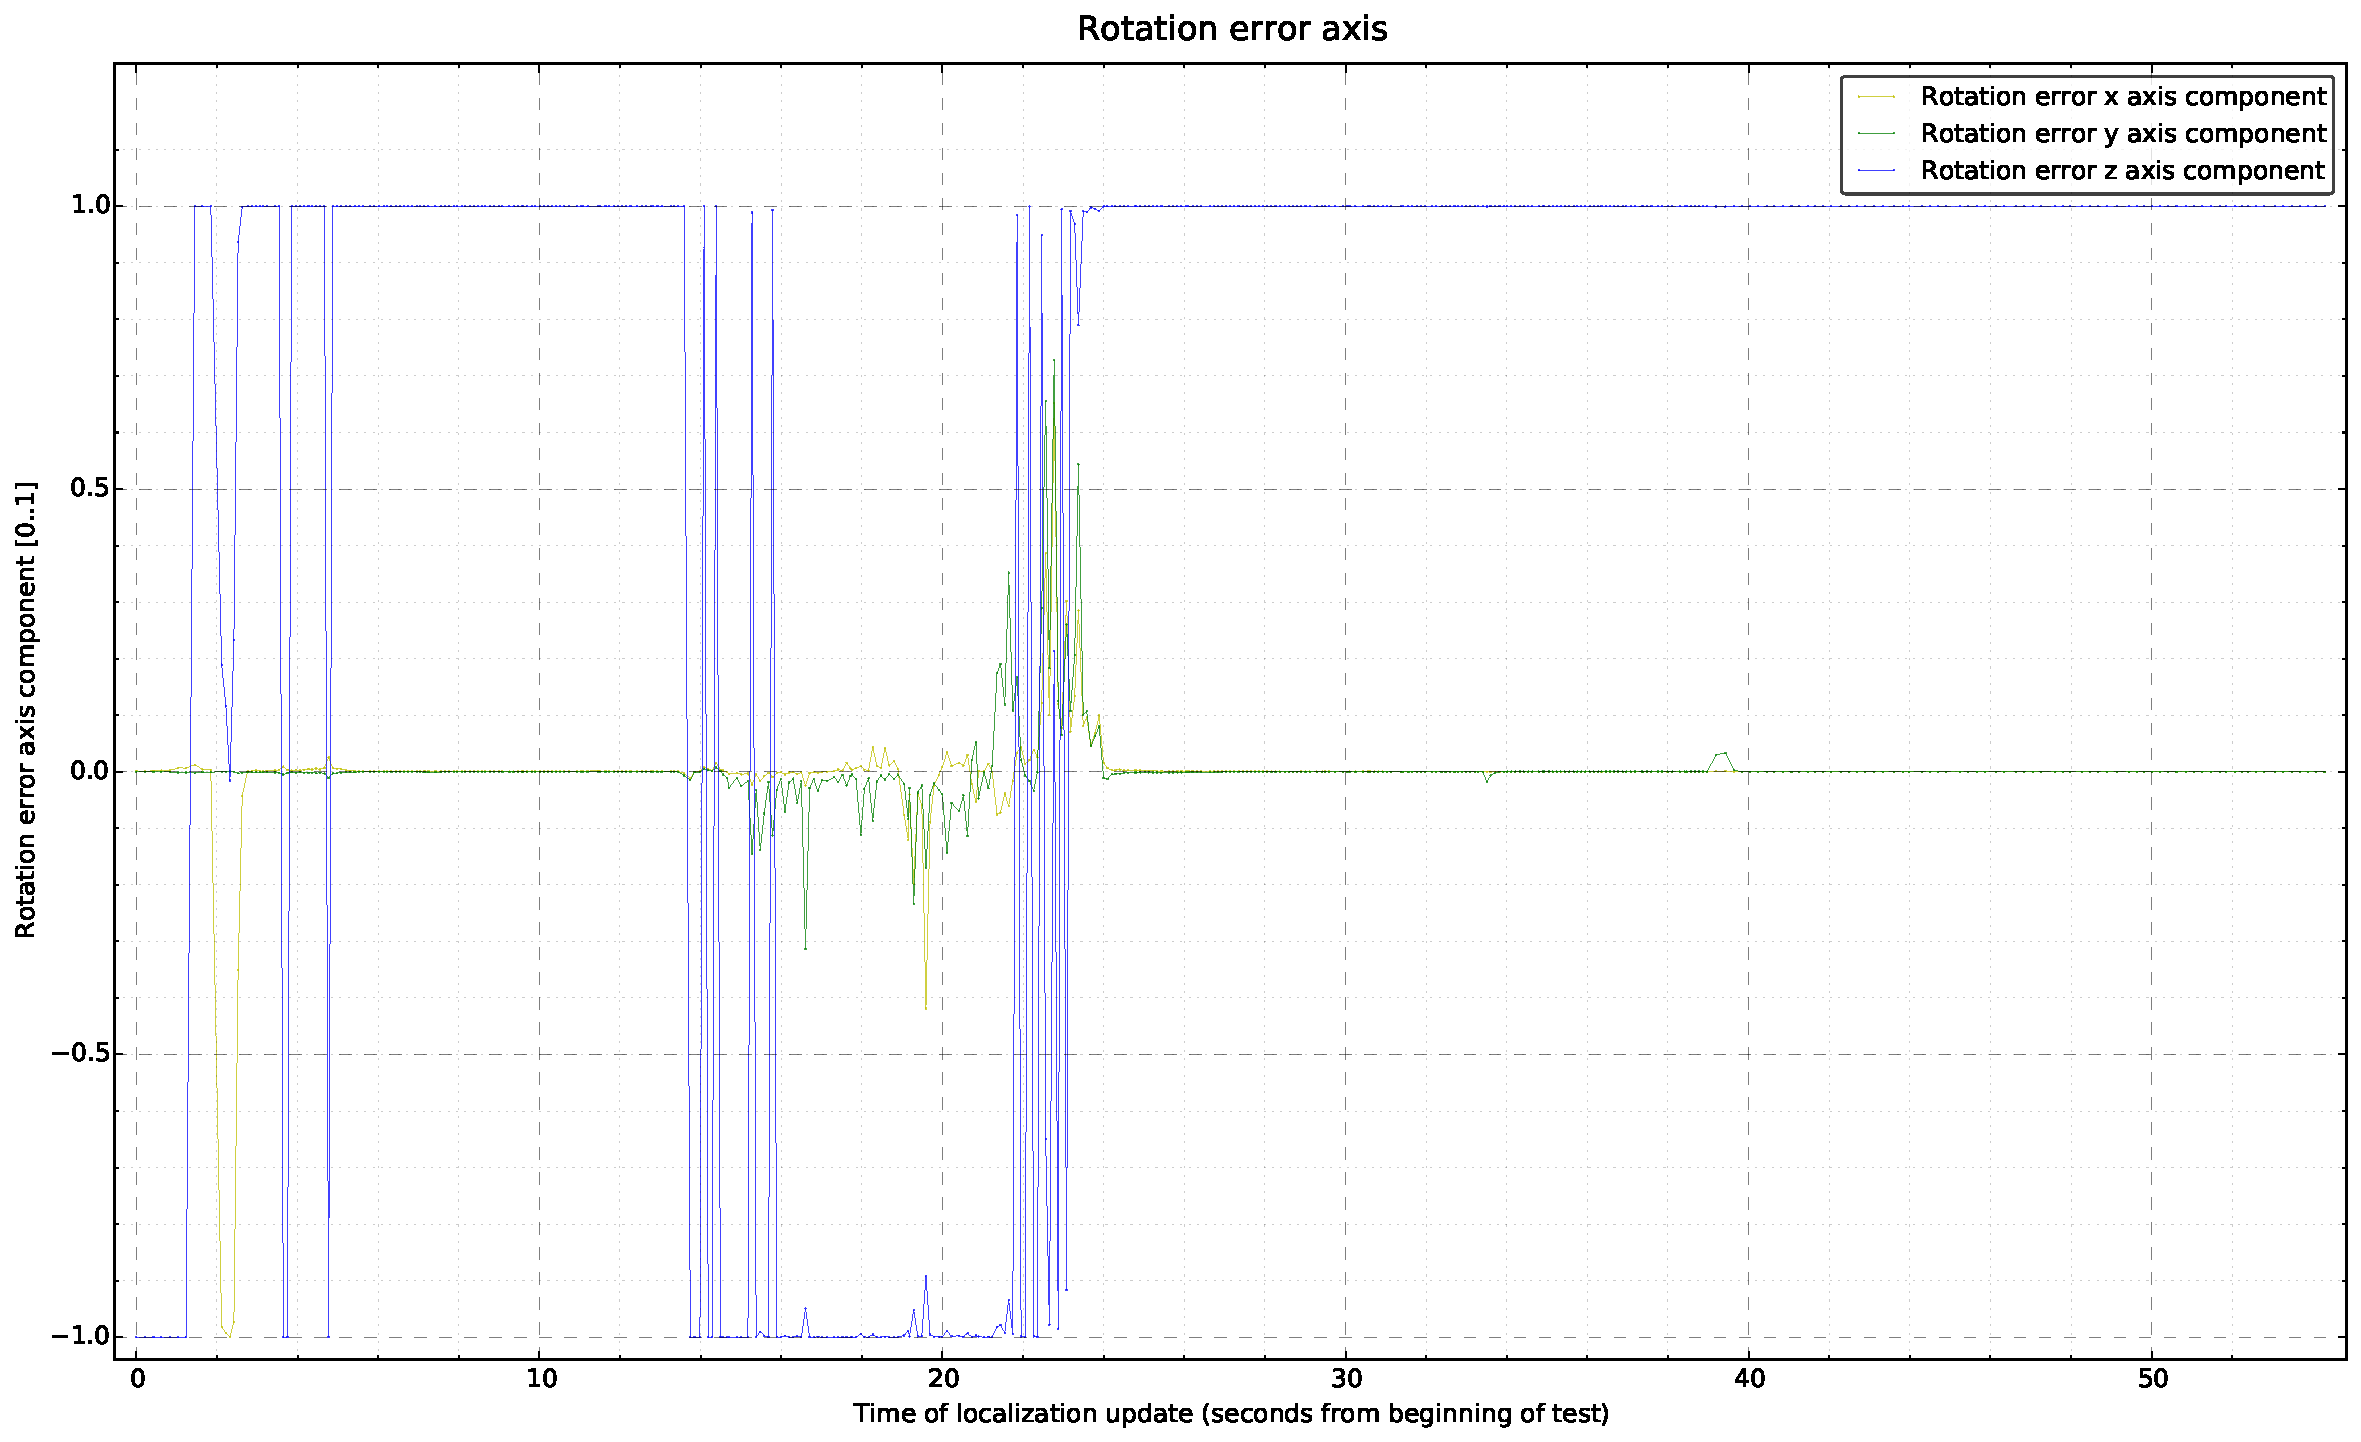
\includegraphics[width=0.69\textwidth]{appendices/tests-3dof/jarvis-robot/\currfilebase/graphs/odometry-rotation-error-axis}
	\caption{Odometry rotation errors axis}
\end{figure}

\begin{figure}[H]
	\centering
	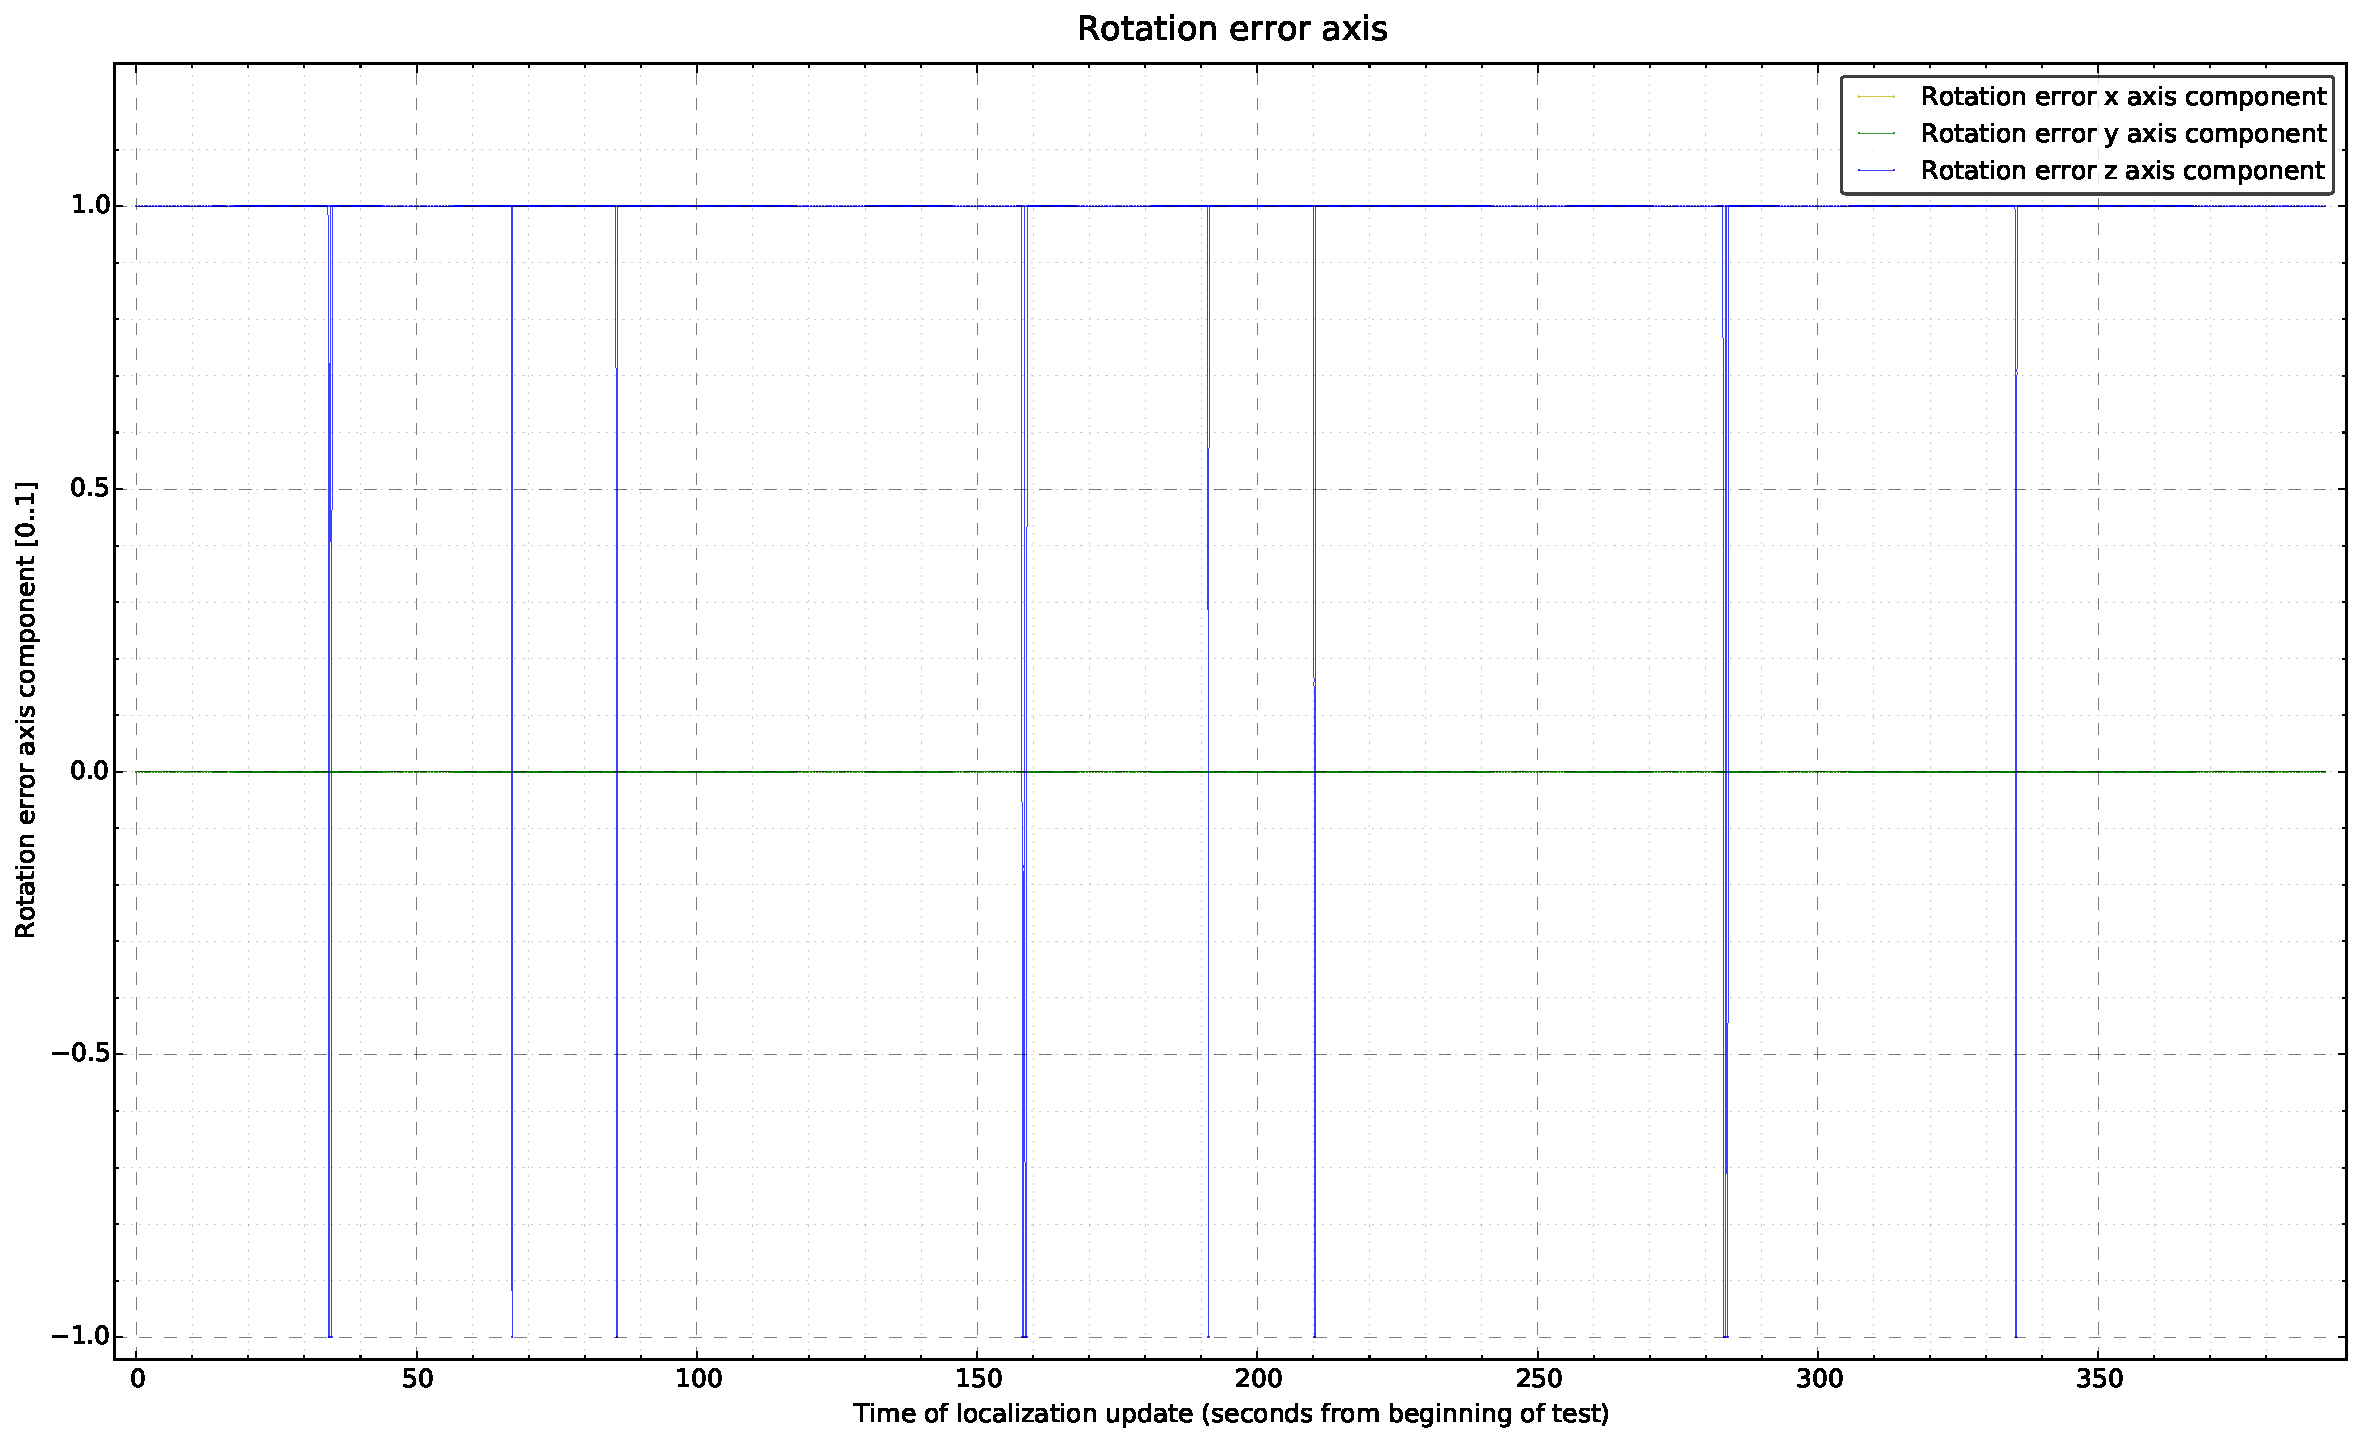
\includegraphics[width=0.69\textwidth]{appendices/tests-3dof/jarvis-robot/\currfilebase/graphs/rotation-error-axis}
	\caption{Localization system rotation errors axis}
\end{figure}

\begin{figure}[H]
	\centering
	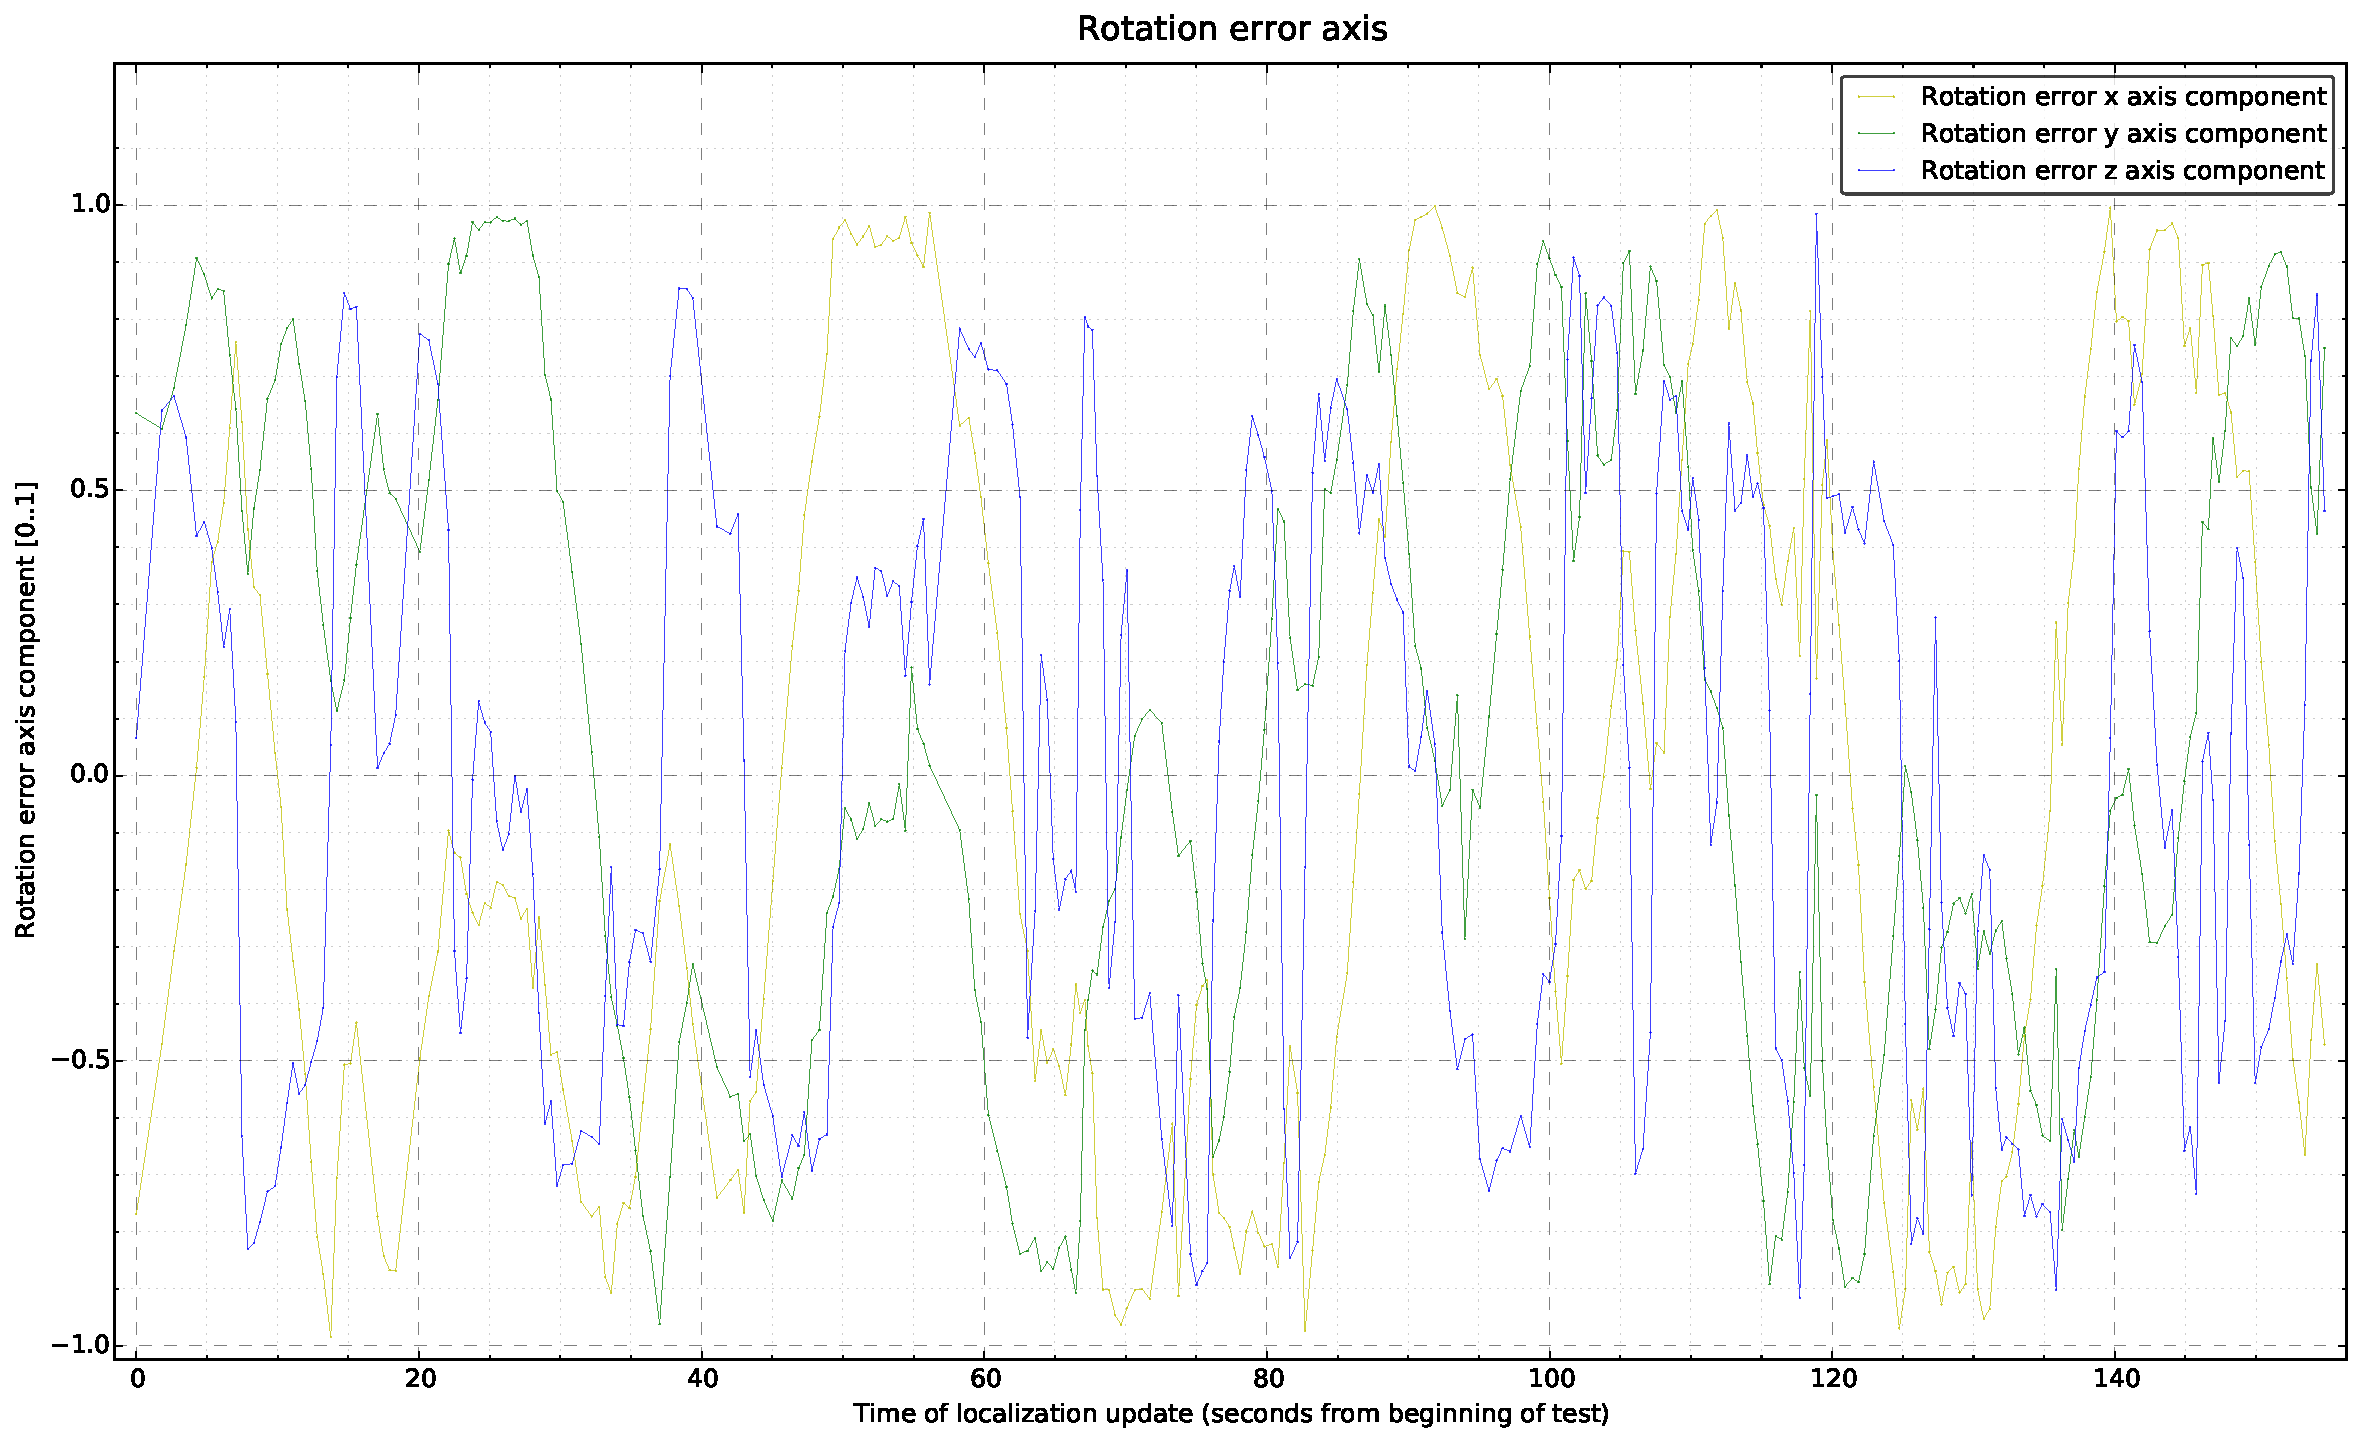
\includegraphics[width=0.69\textwidth]{appendices/tests-3dof/jarvis-robot/\currfilebase/graphs/rotation-error-axis-amcl}
	\caption{\glsentrytext{amcl} rotation errors axis}
\end{figure}


%Angular errors
\begin{figure}[H]
	\centering
	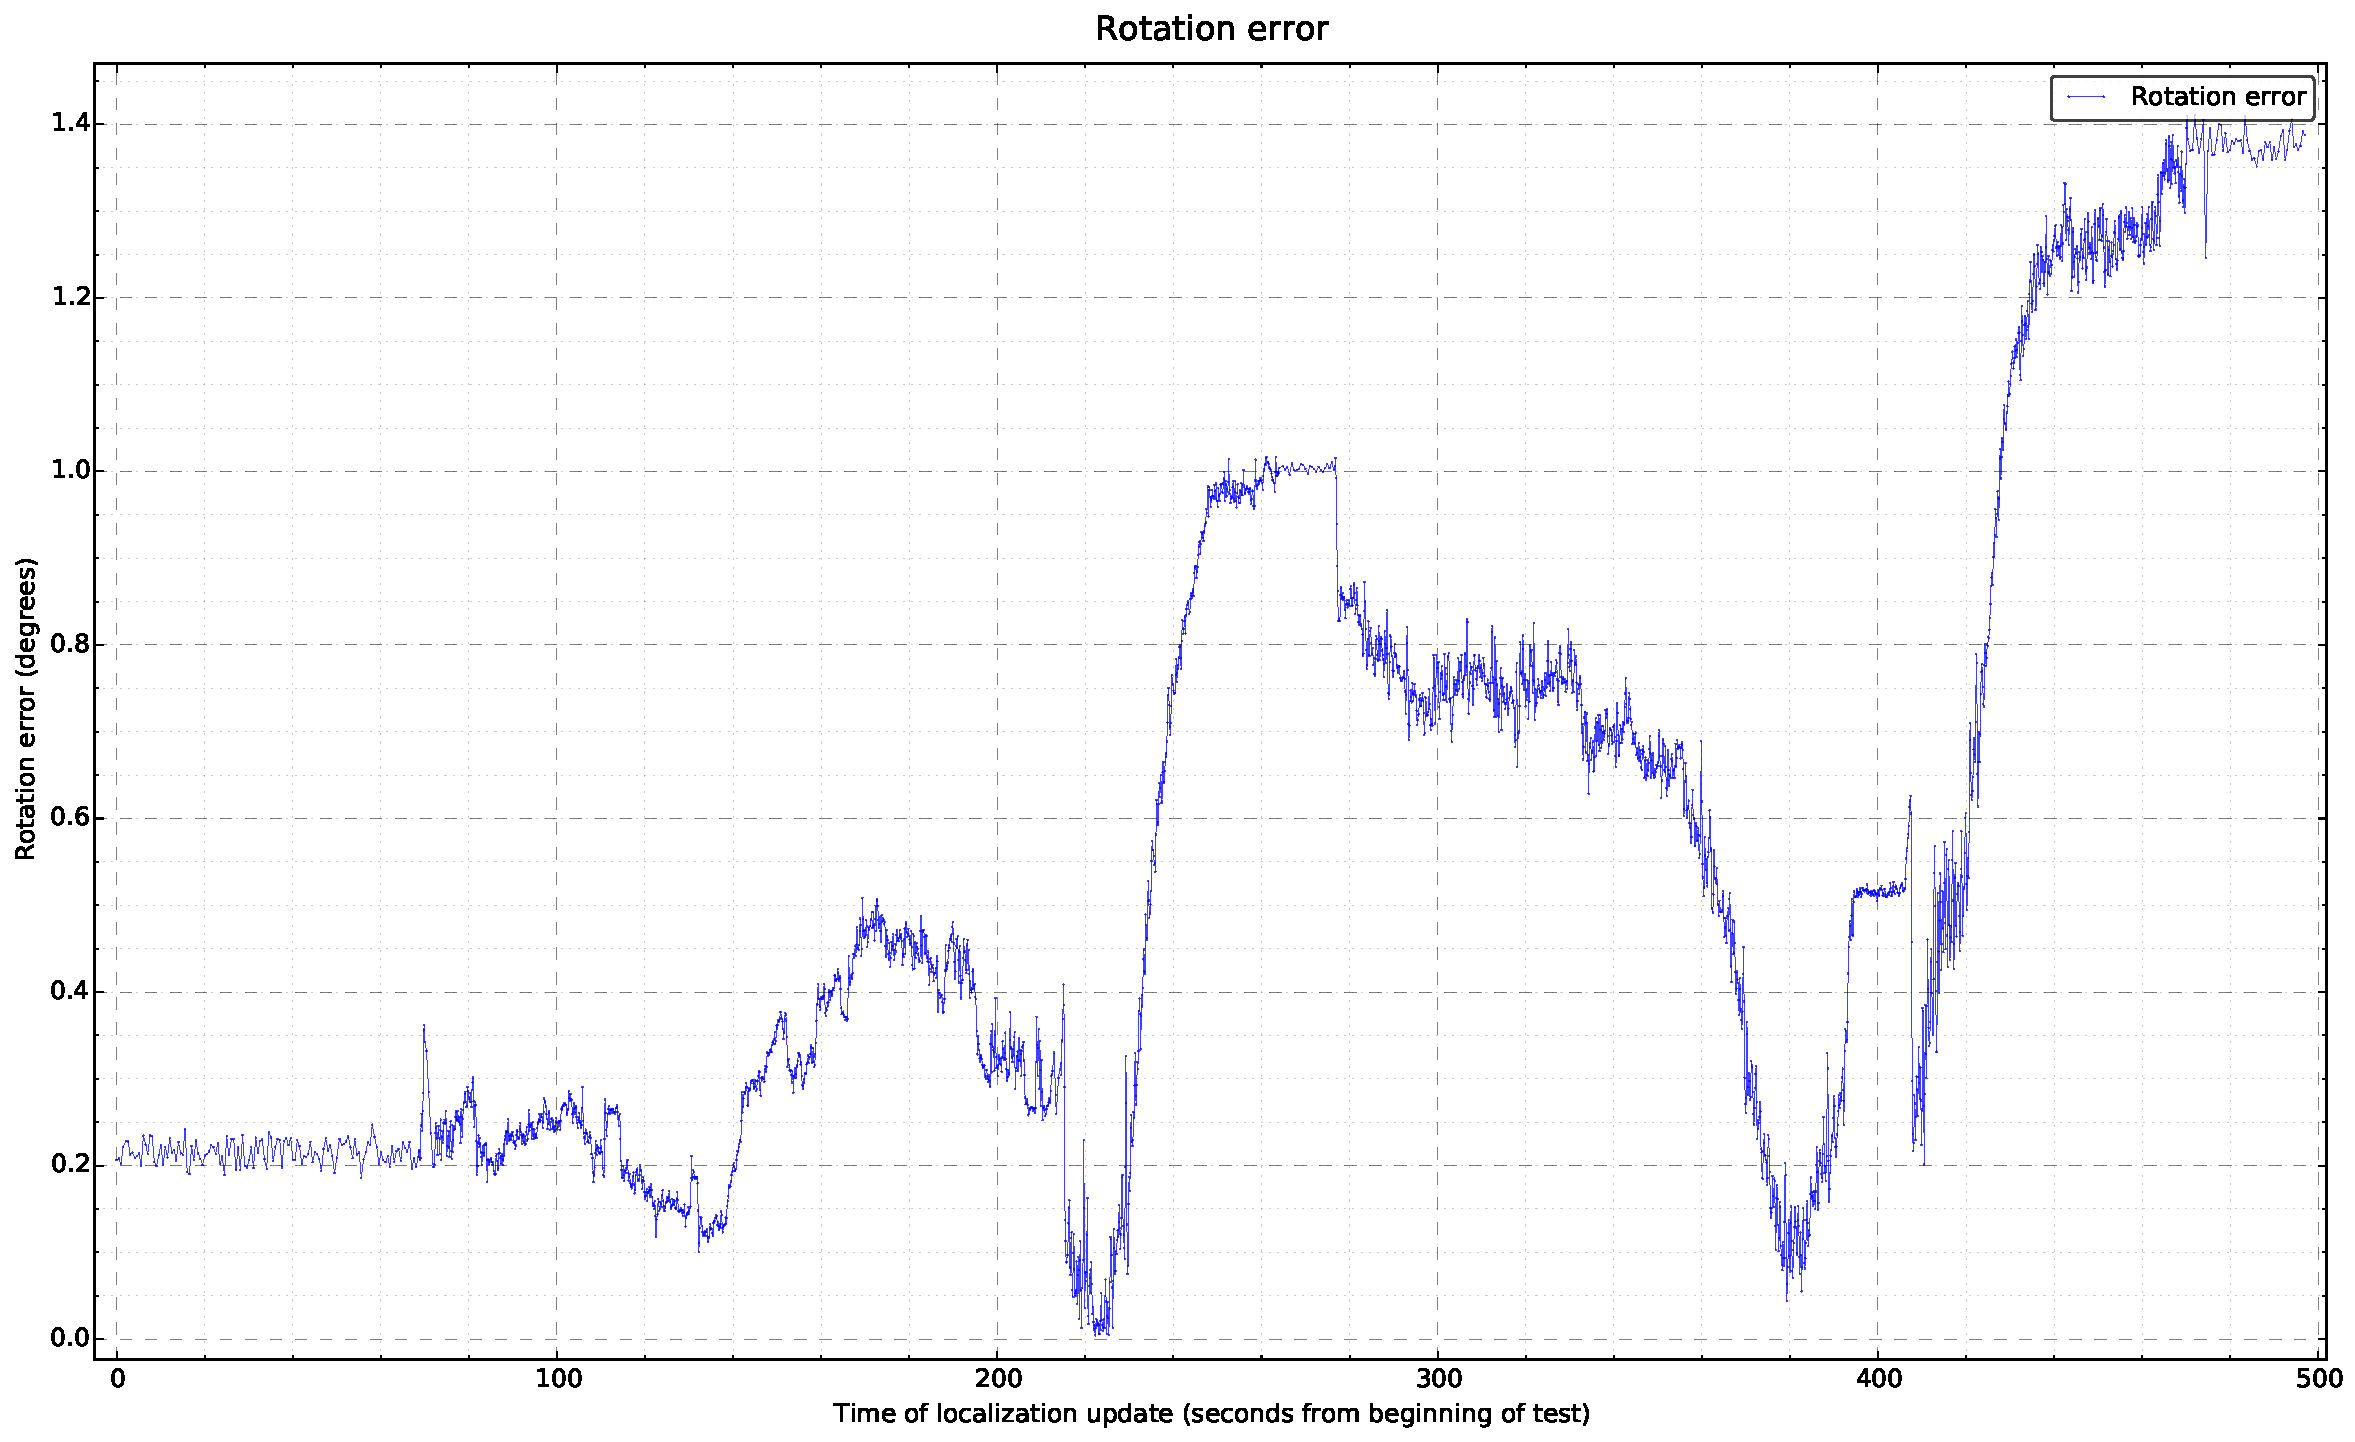
\includegraphics[width=0.69\textwidth]{appendices/tests-3dof/jarvis-robot/\currfilebase/graphs/odometry-rotation-error-degrees}
	\caption{Odometry rotation errors}
\end{figure}

\begin{figure}[H]
	\centering
	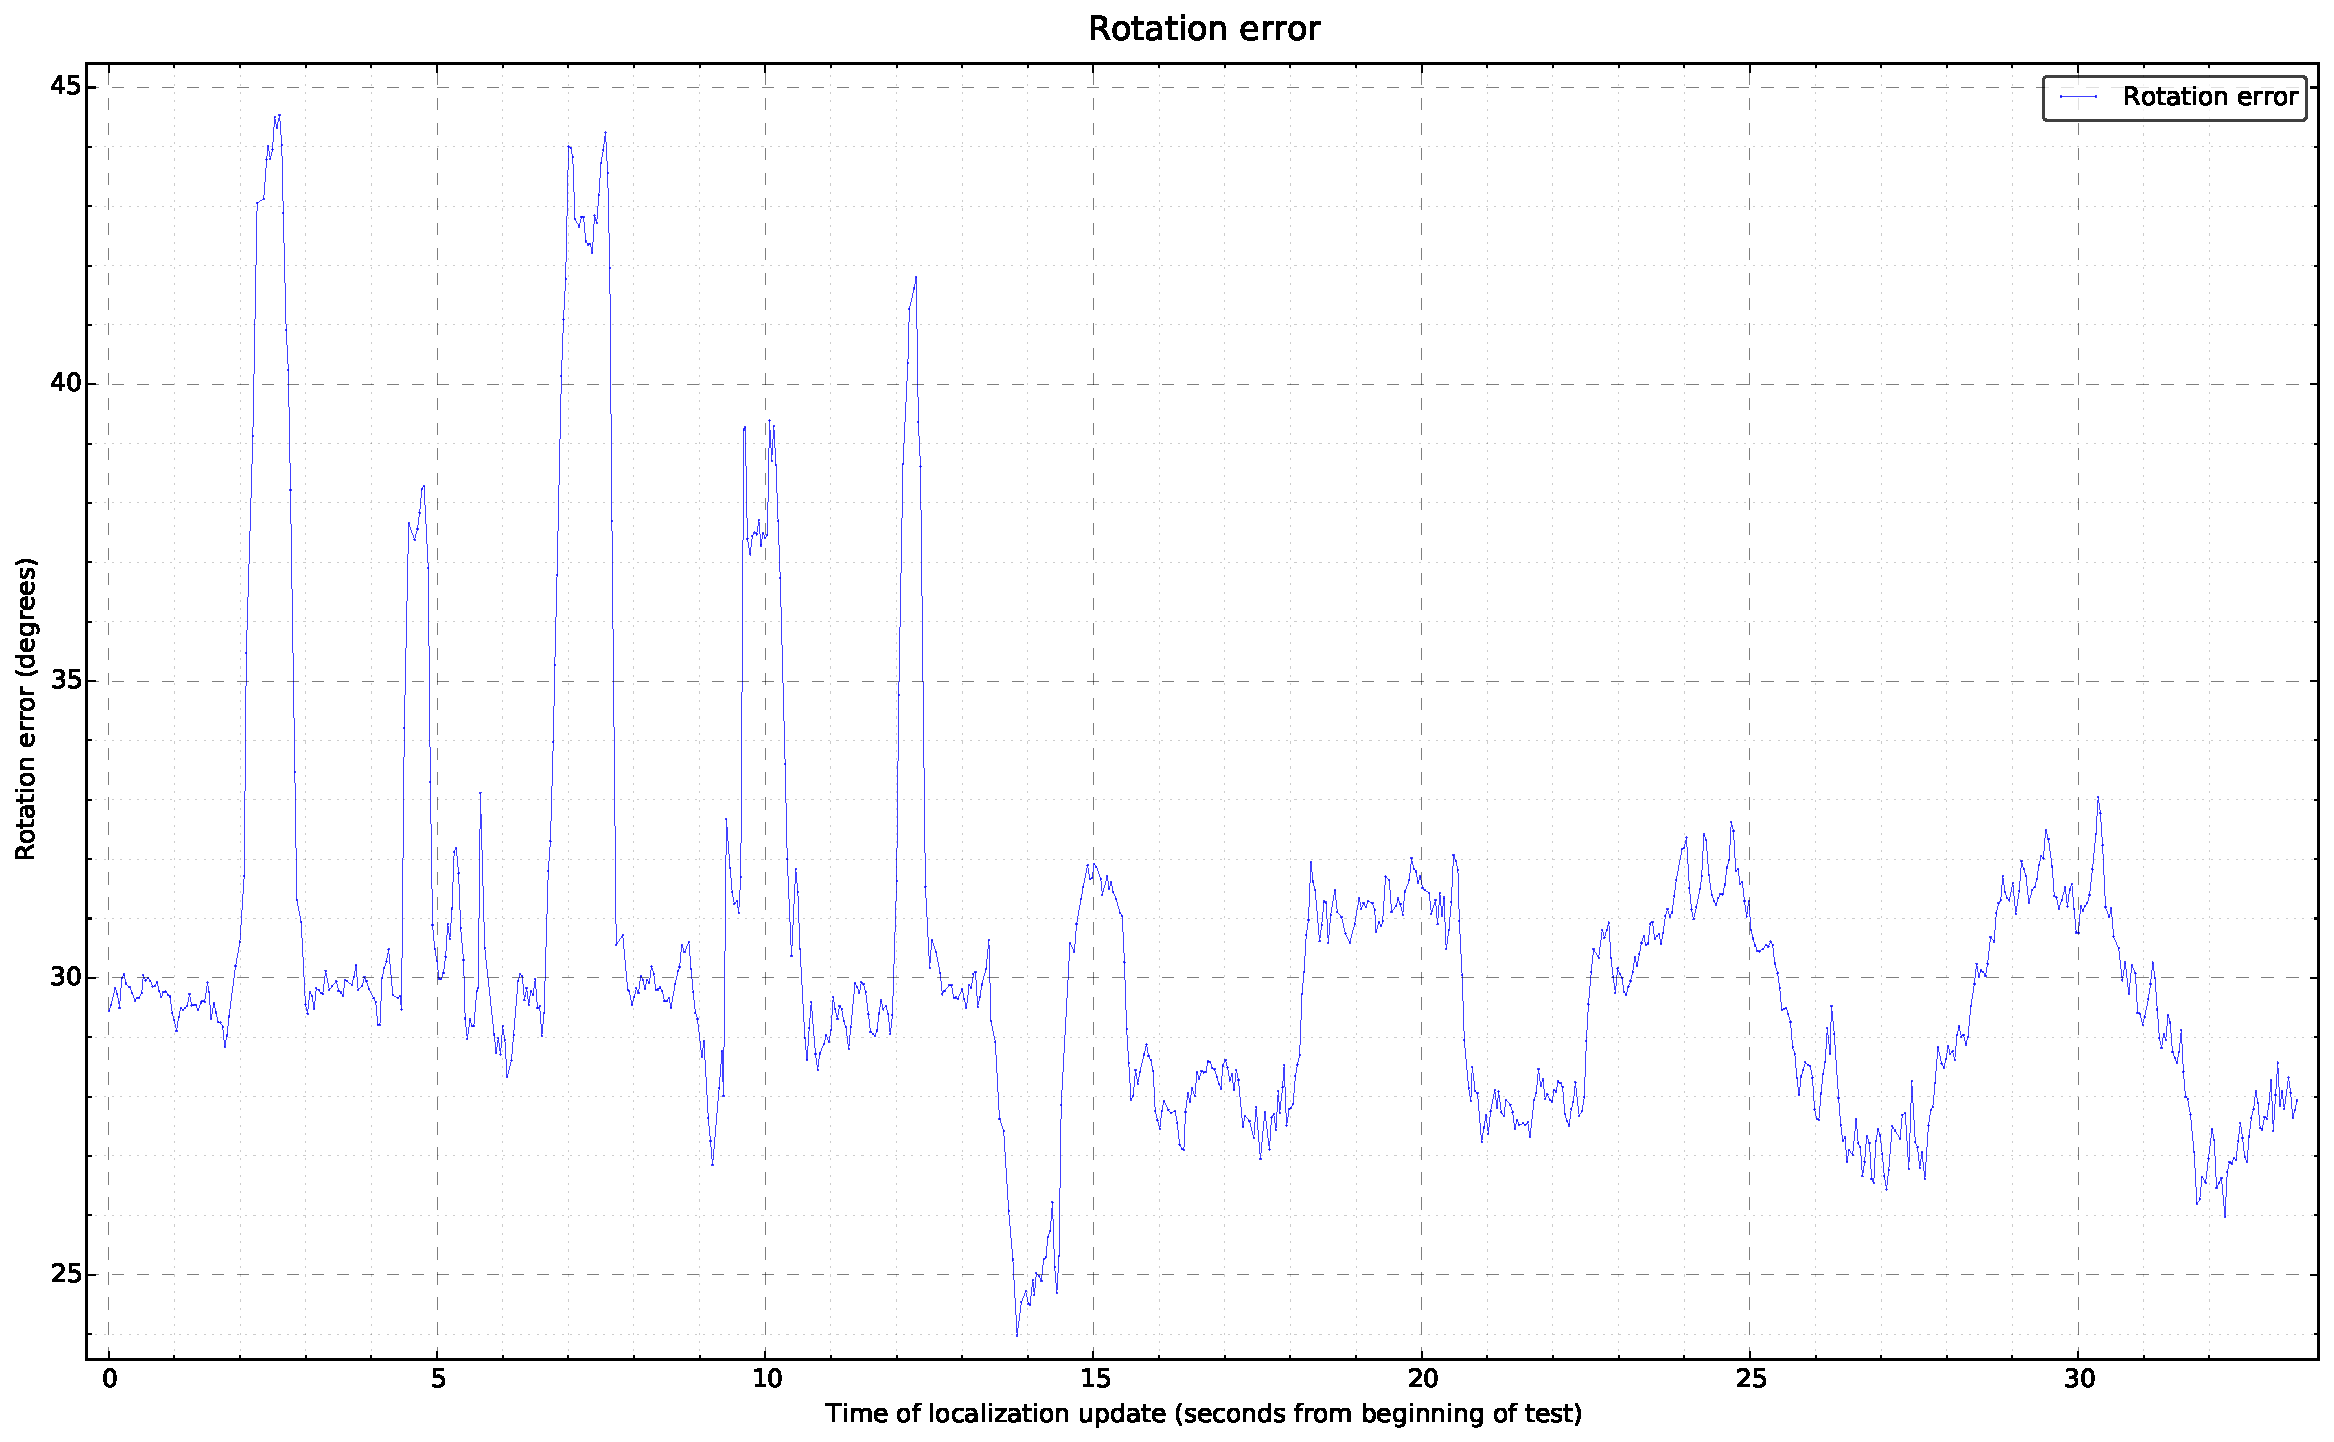
\includegraphics[width=0.69\textwidth]{appendices/tests-3dof/jarvis-robot/\currfilebase/graphs/rotation-error-degrees}
	\caption{Localization system rotation errors}
\end{figure}

\begin{figure}[H]
	\centering
	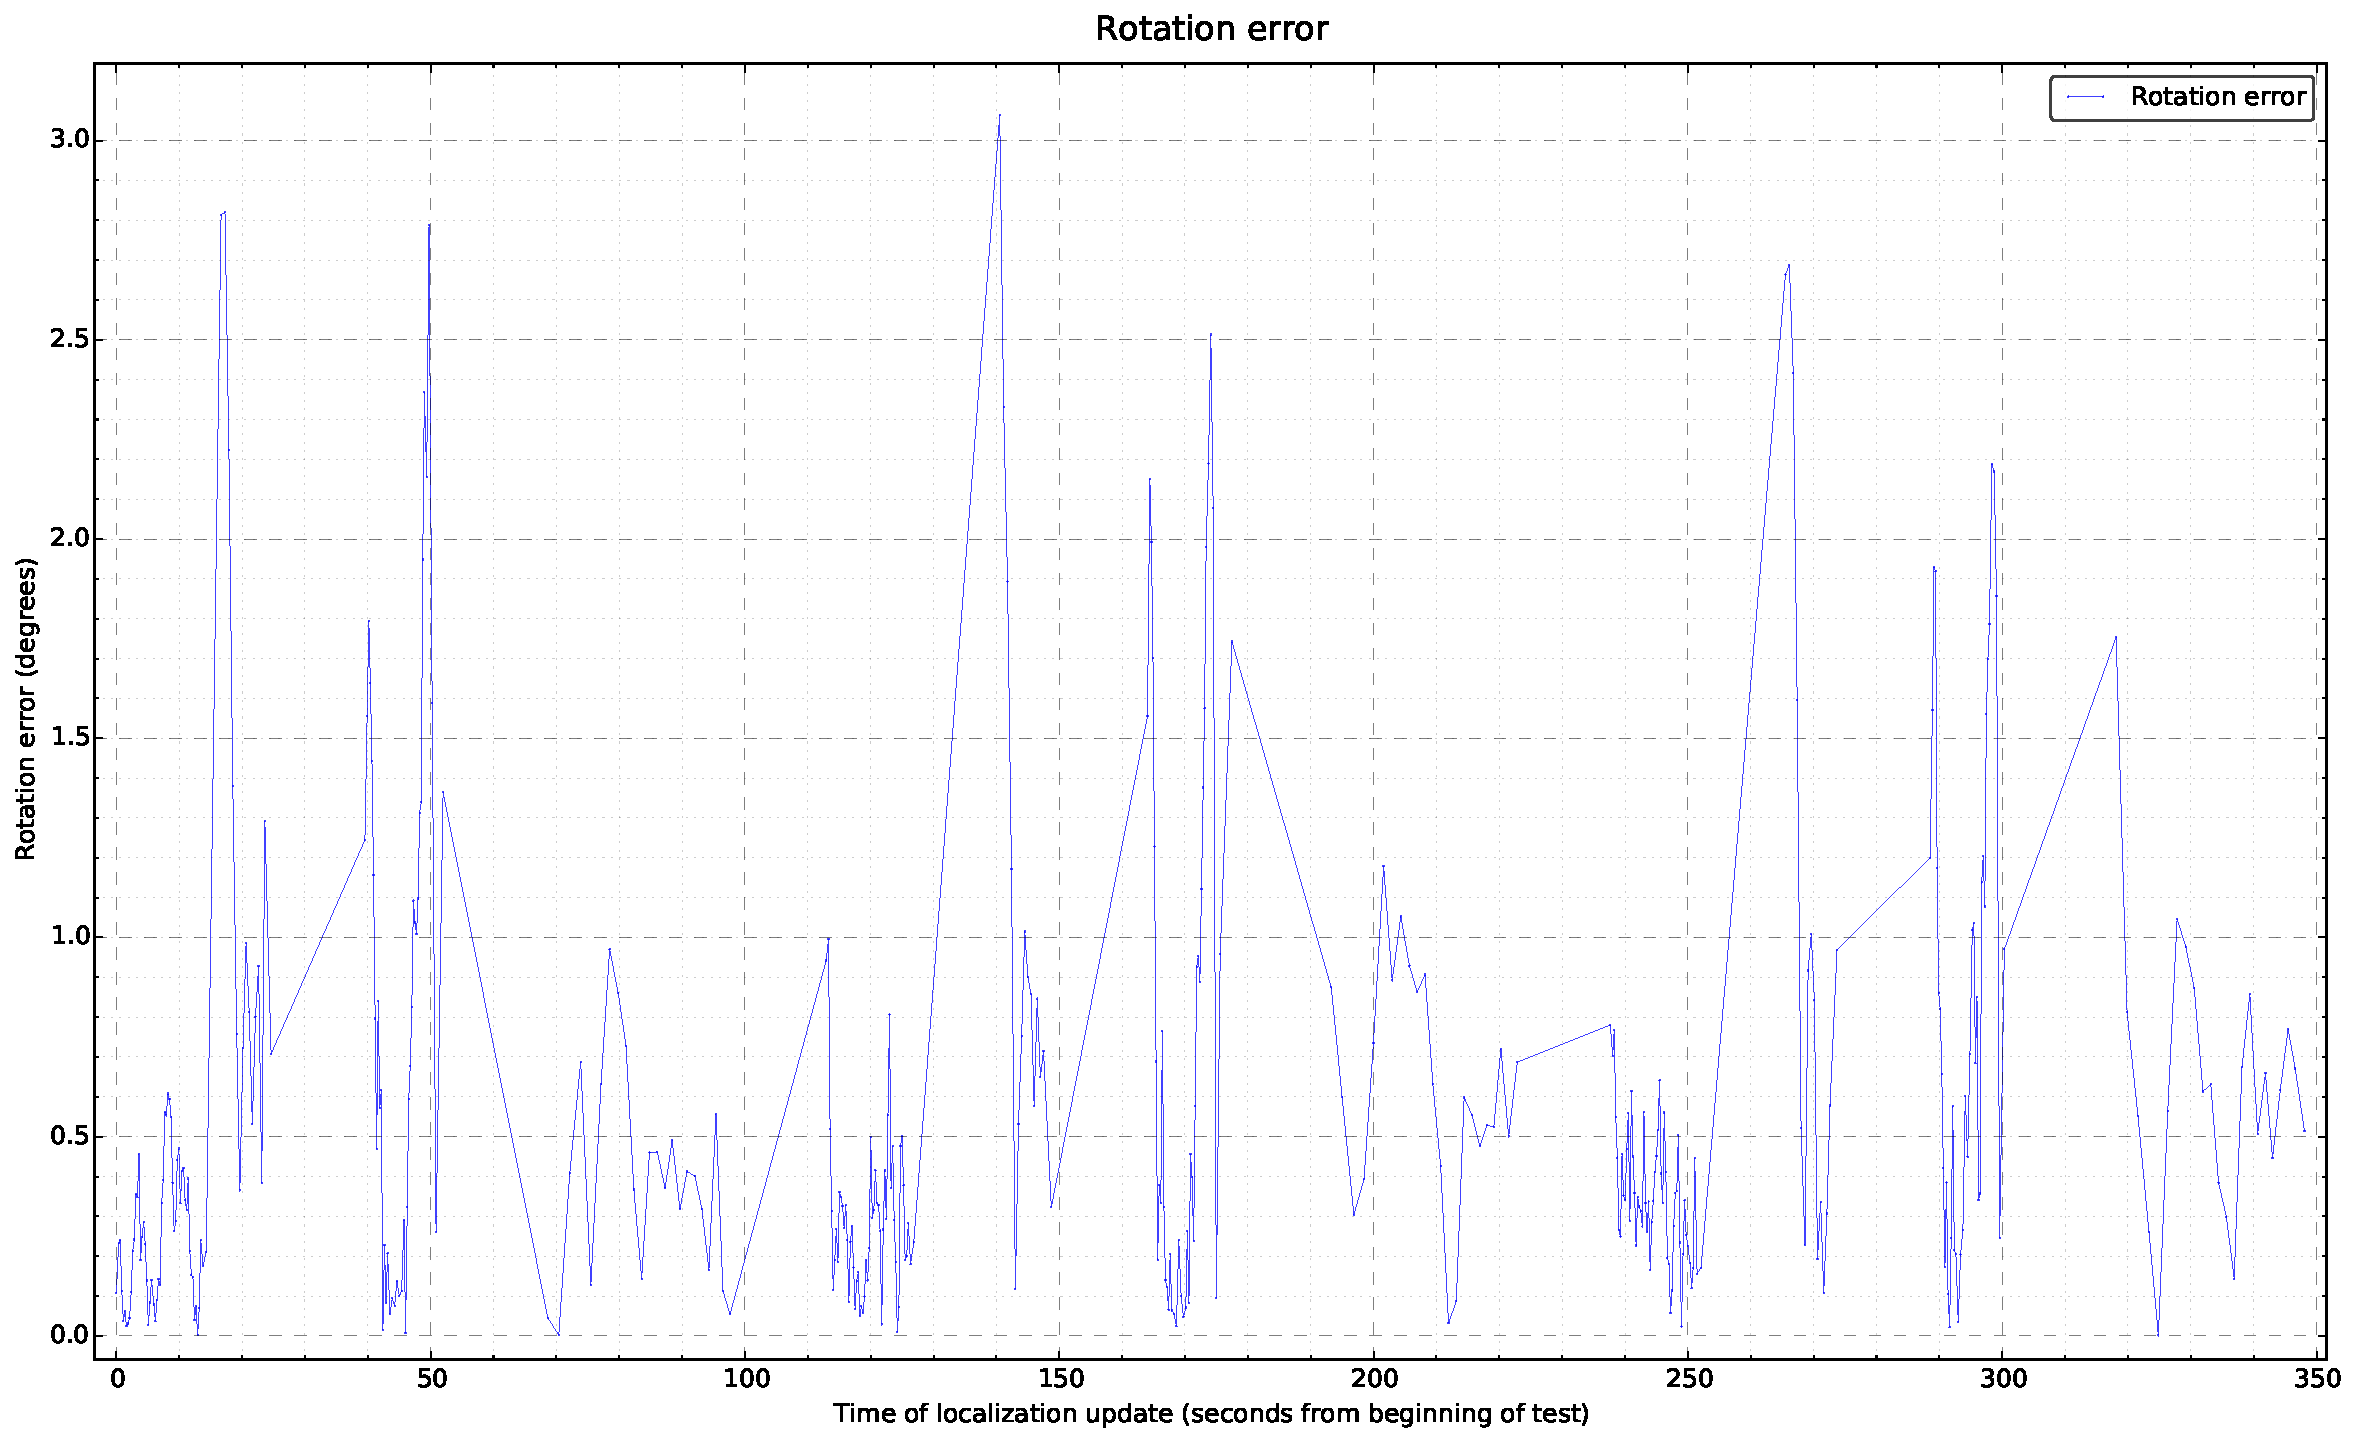
\includegraphics[width=0.69\textwidth]{appendices/tests-3dof/jarvis-robot/\currfilebase/graphs/rotation-error-degrees-amcl}
	\caption{\glsentrytext{amcl} rotation errors}
\end{figure}


%Angular errors distributions
\begin{figure}[H]
	\centering
	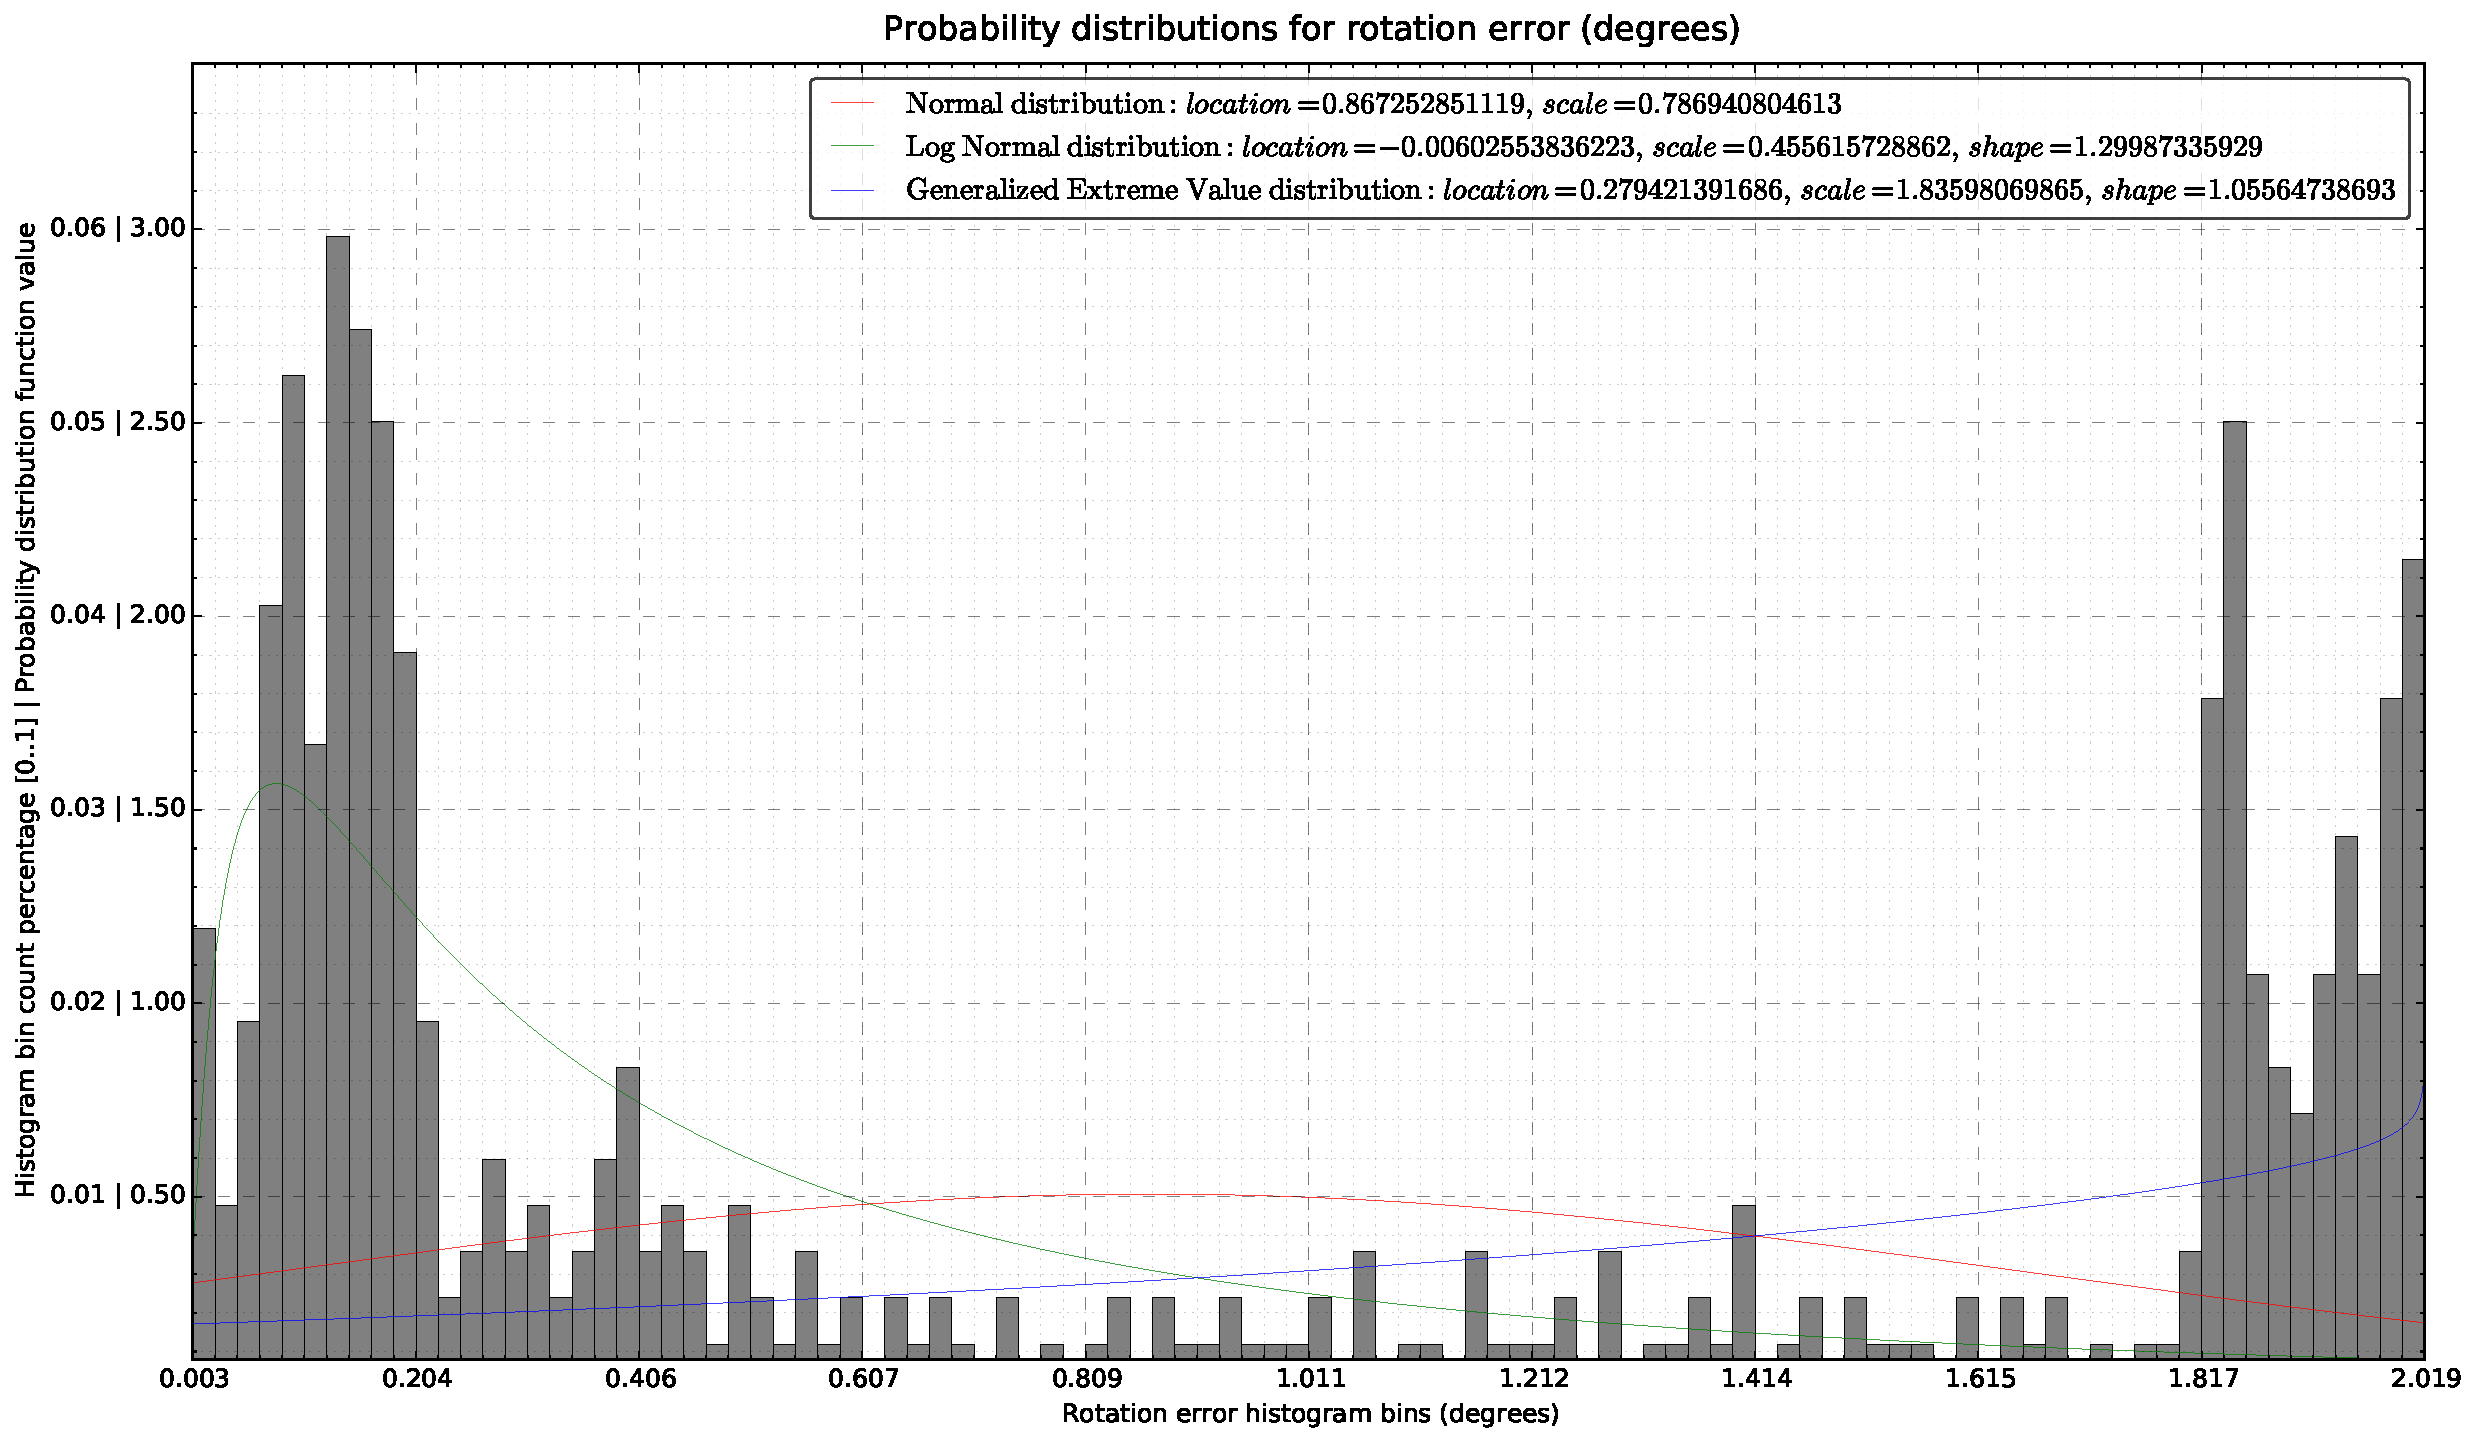
\includegraphics[width=0.73\textwidth]{appendices/tests-3dof/jarvis-robot/\currfilebase/graphs/odometry-rotation-error-degrees-distributions}
	\caption{Probability distributions for the odometry rotation errors}
\end{figure}

\begin{figure}[H]
	\centering
	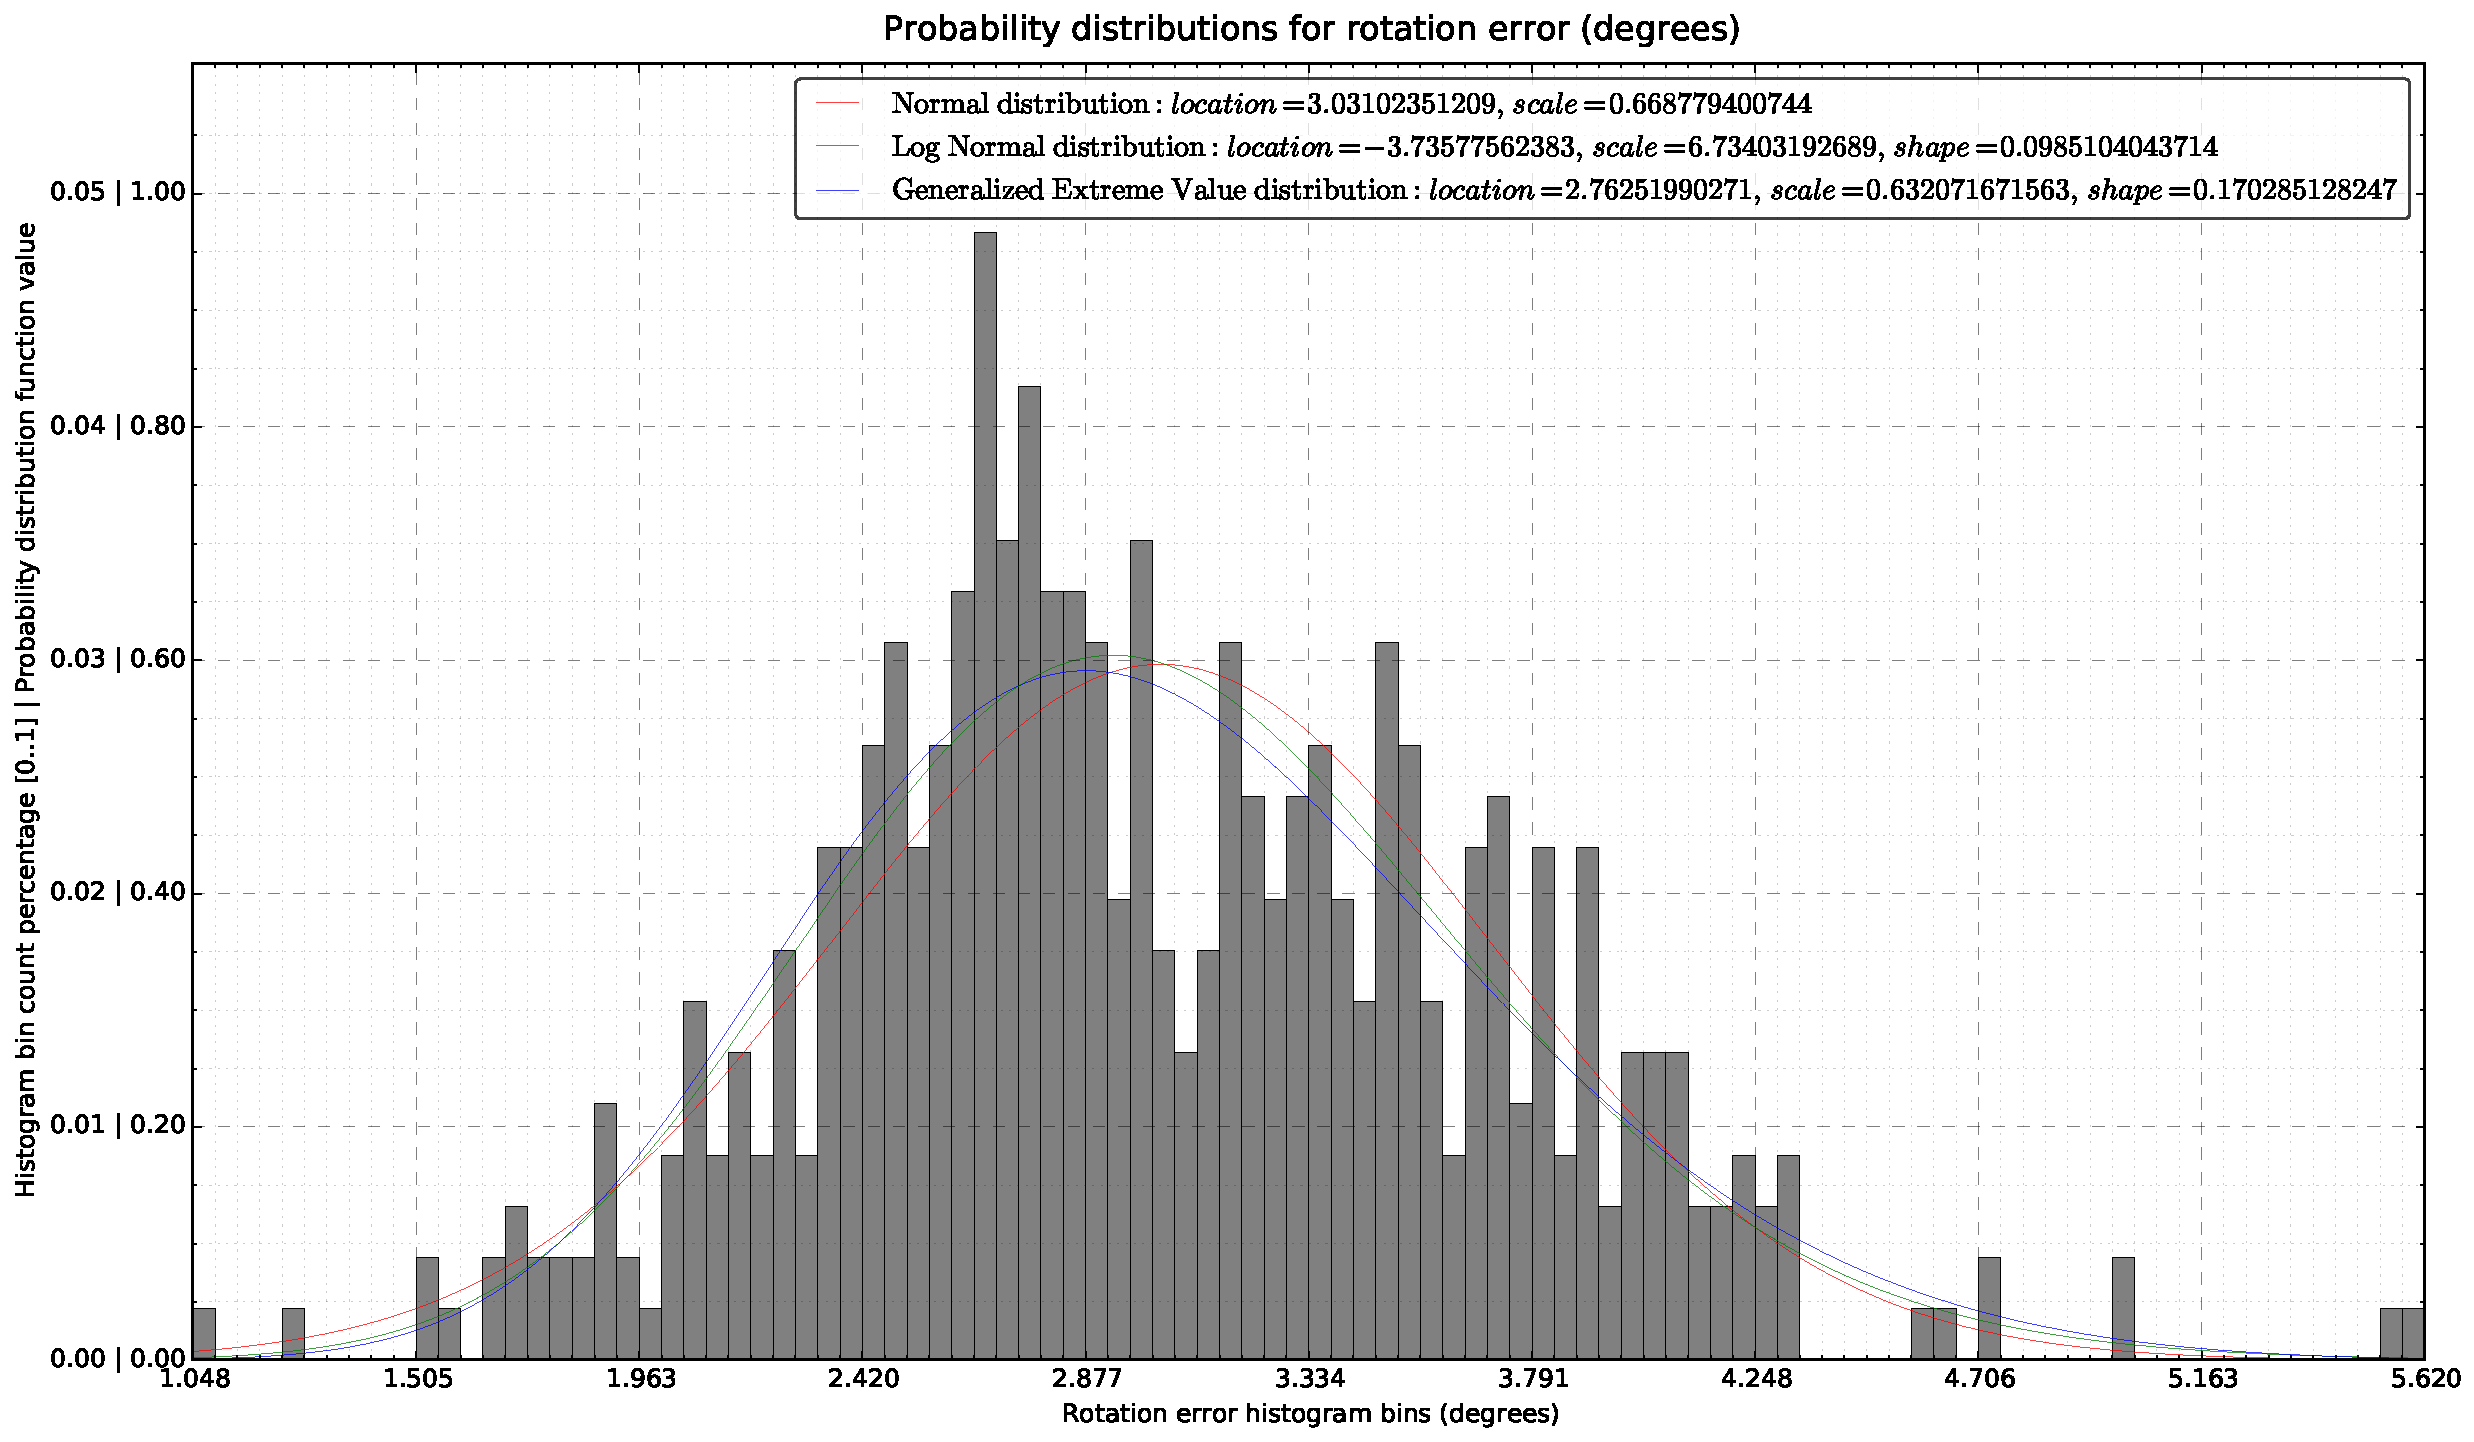
\includegraphics[width=0.73\textwidth]{appendices/tests-3dof/jarvis-robot/\currfilebase/graphs/rotation-error-degrees-distributions}
	\caption{Probability distributions for the localization system rotation errors}
\end{figure}

\begin{figure}[H]
	\centering
	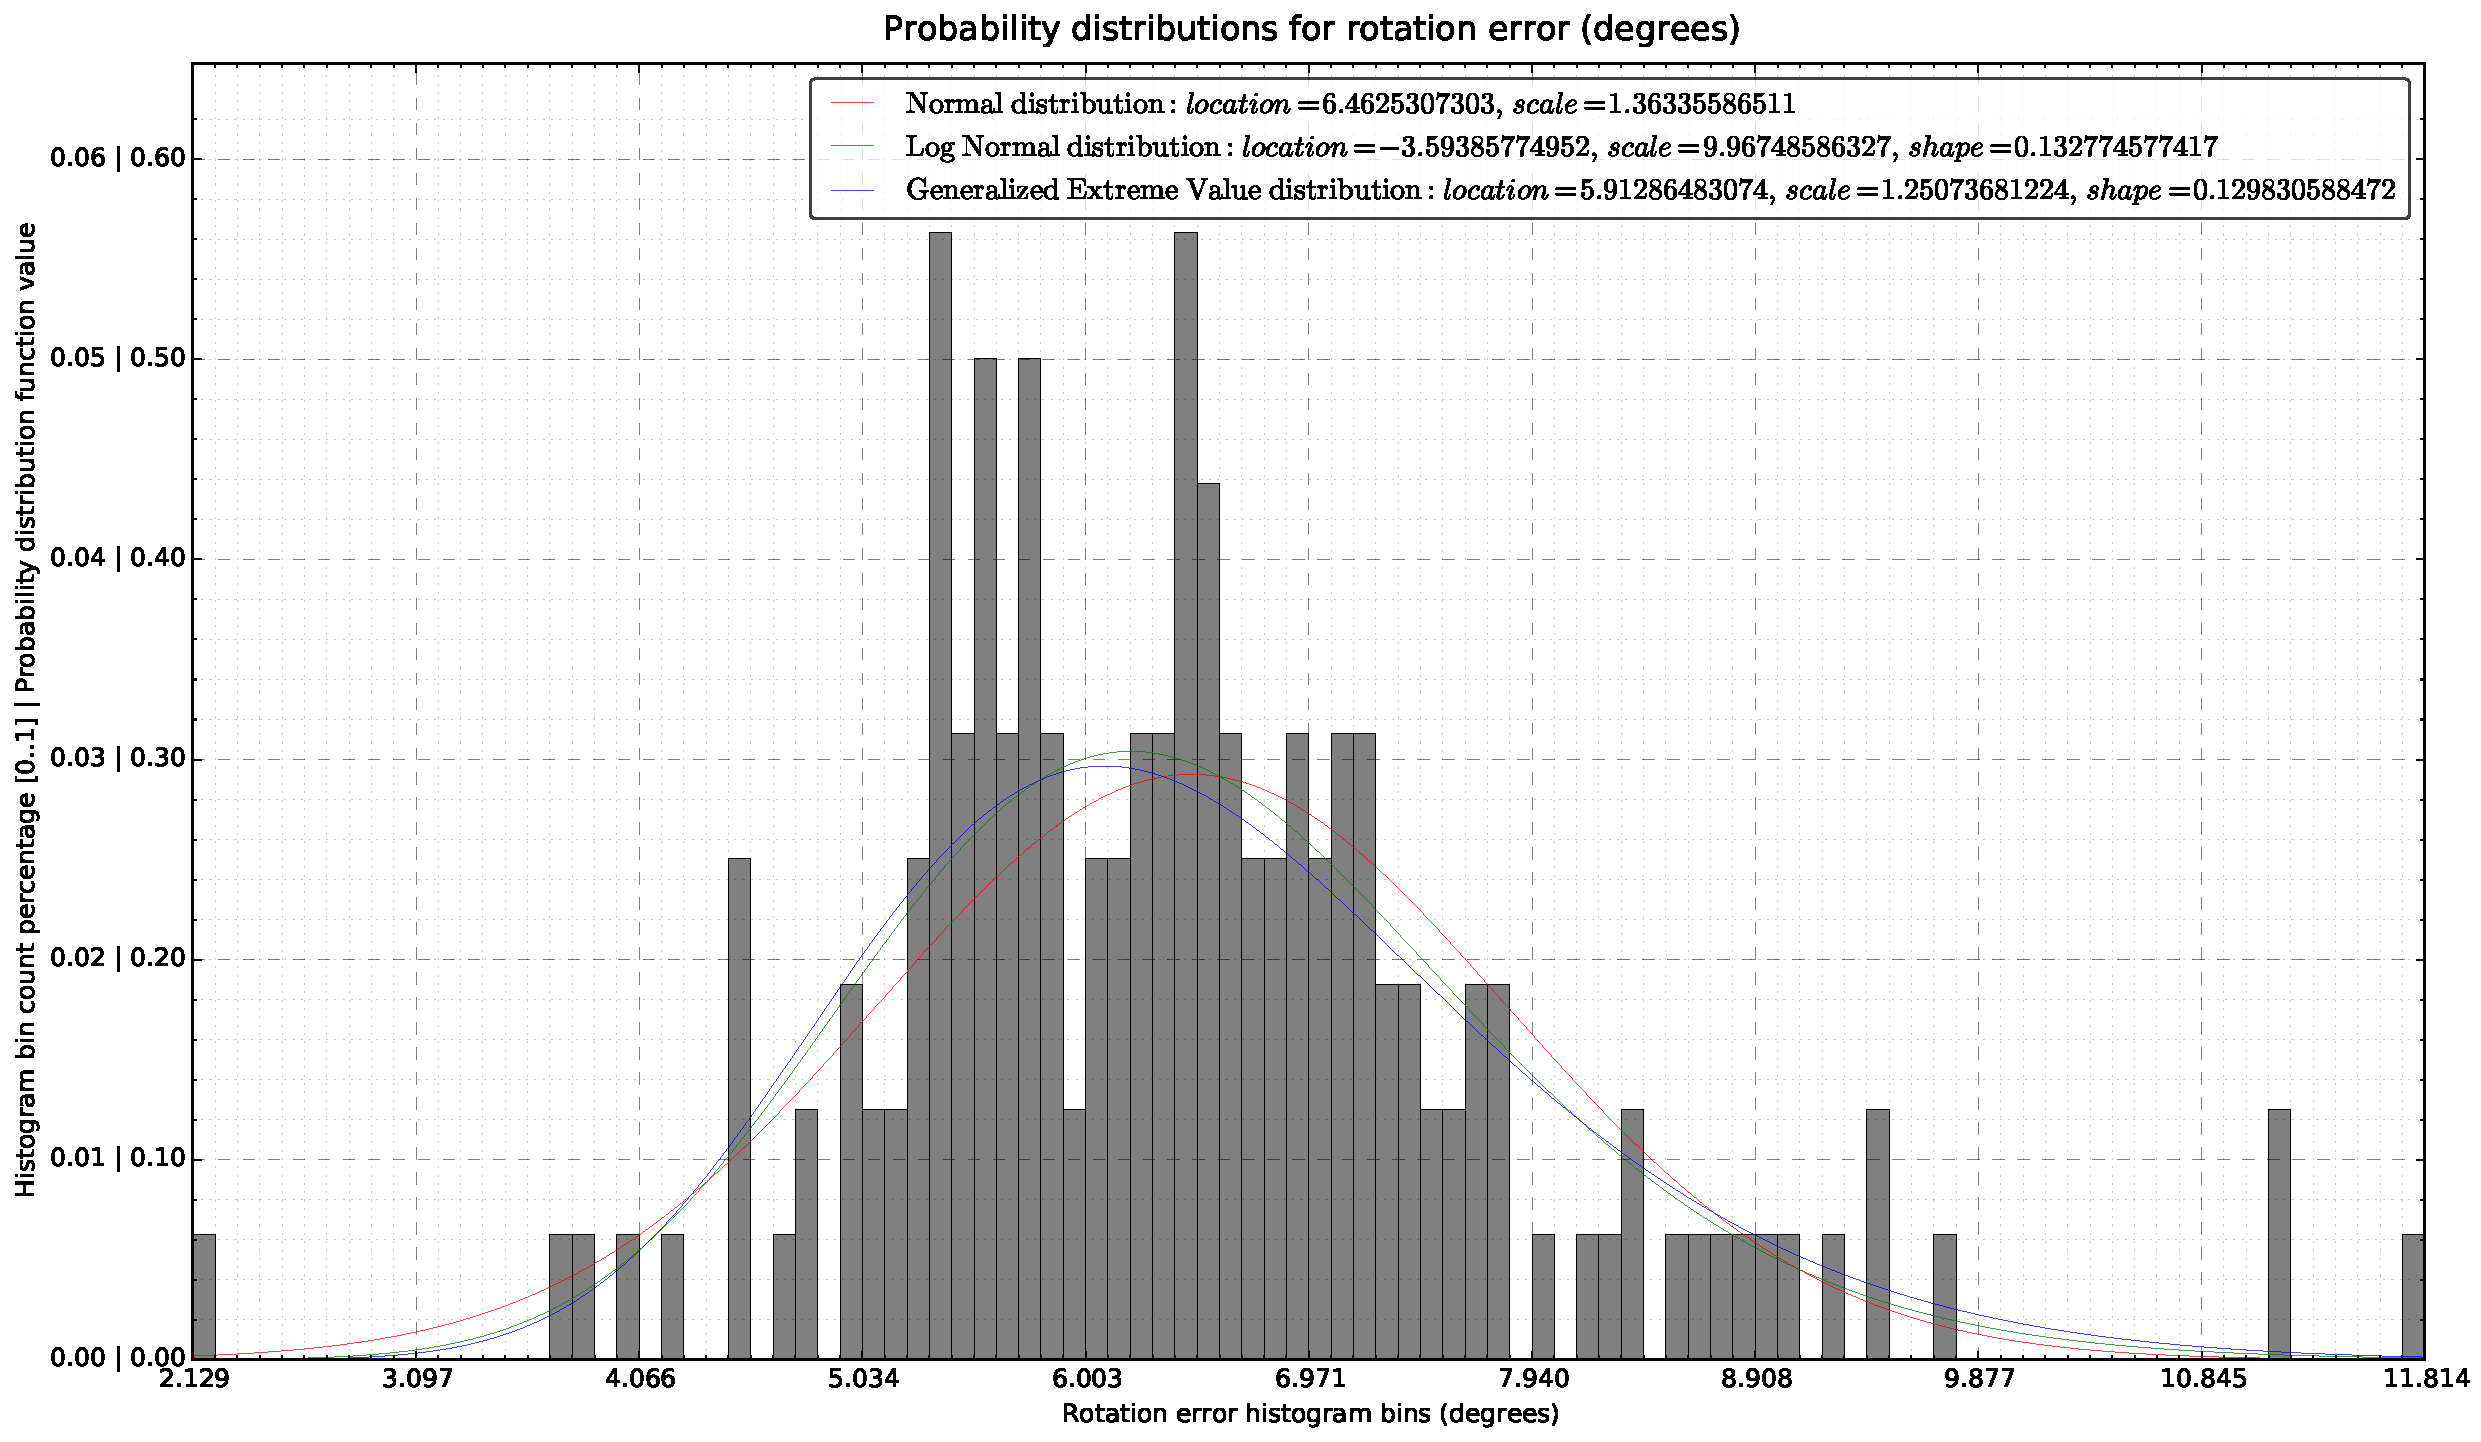
\includegraphics[width=0.73\textwidth]{appendices/tests-3dof/jarvis-robot/\currfilebase/graphs/rotation-error-degrees-distributions-amcl}
	\caption{Probability distributions for the \glsentrytext{amcl} rotation errors}
\end{figure}


%Translation corrections
\begin{figure}[H]
	\centering
	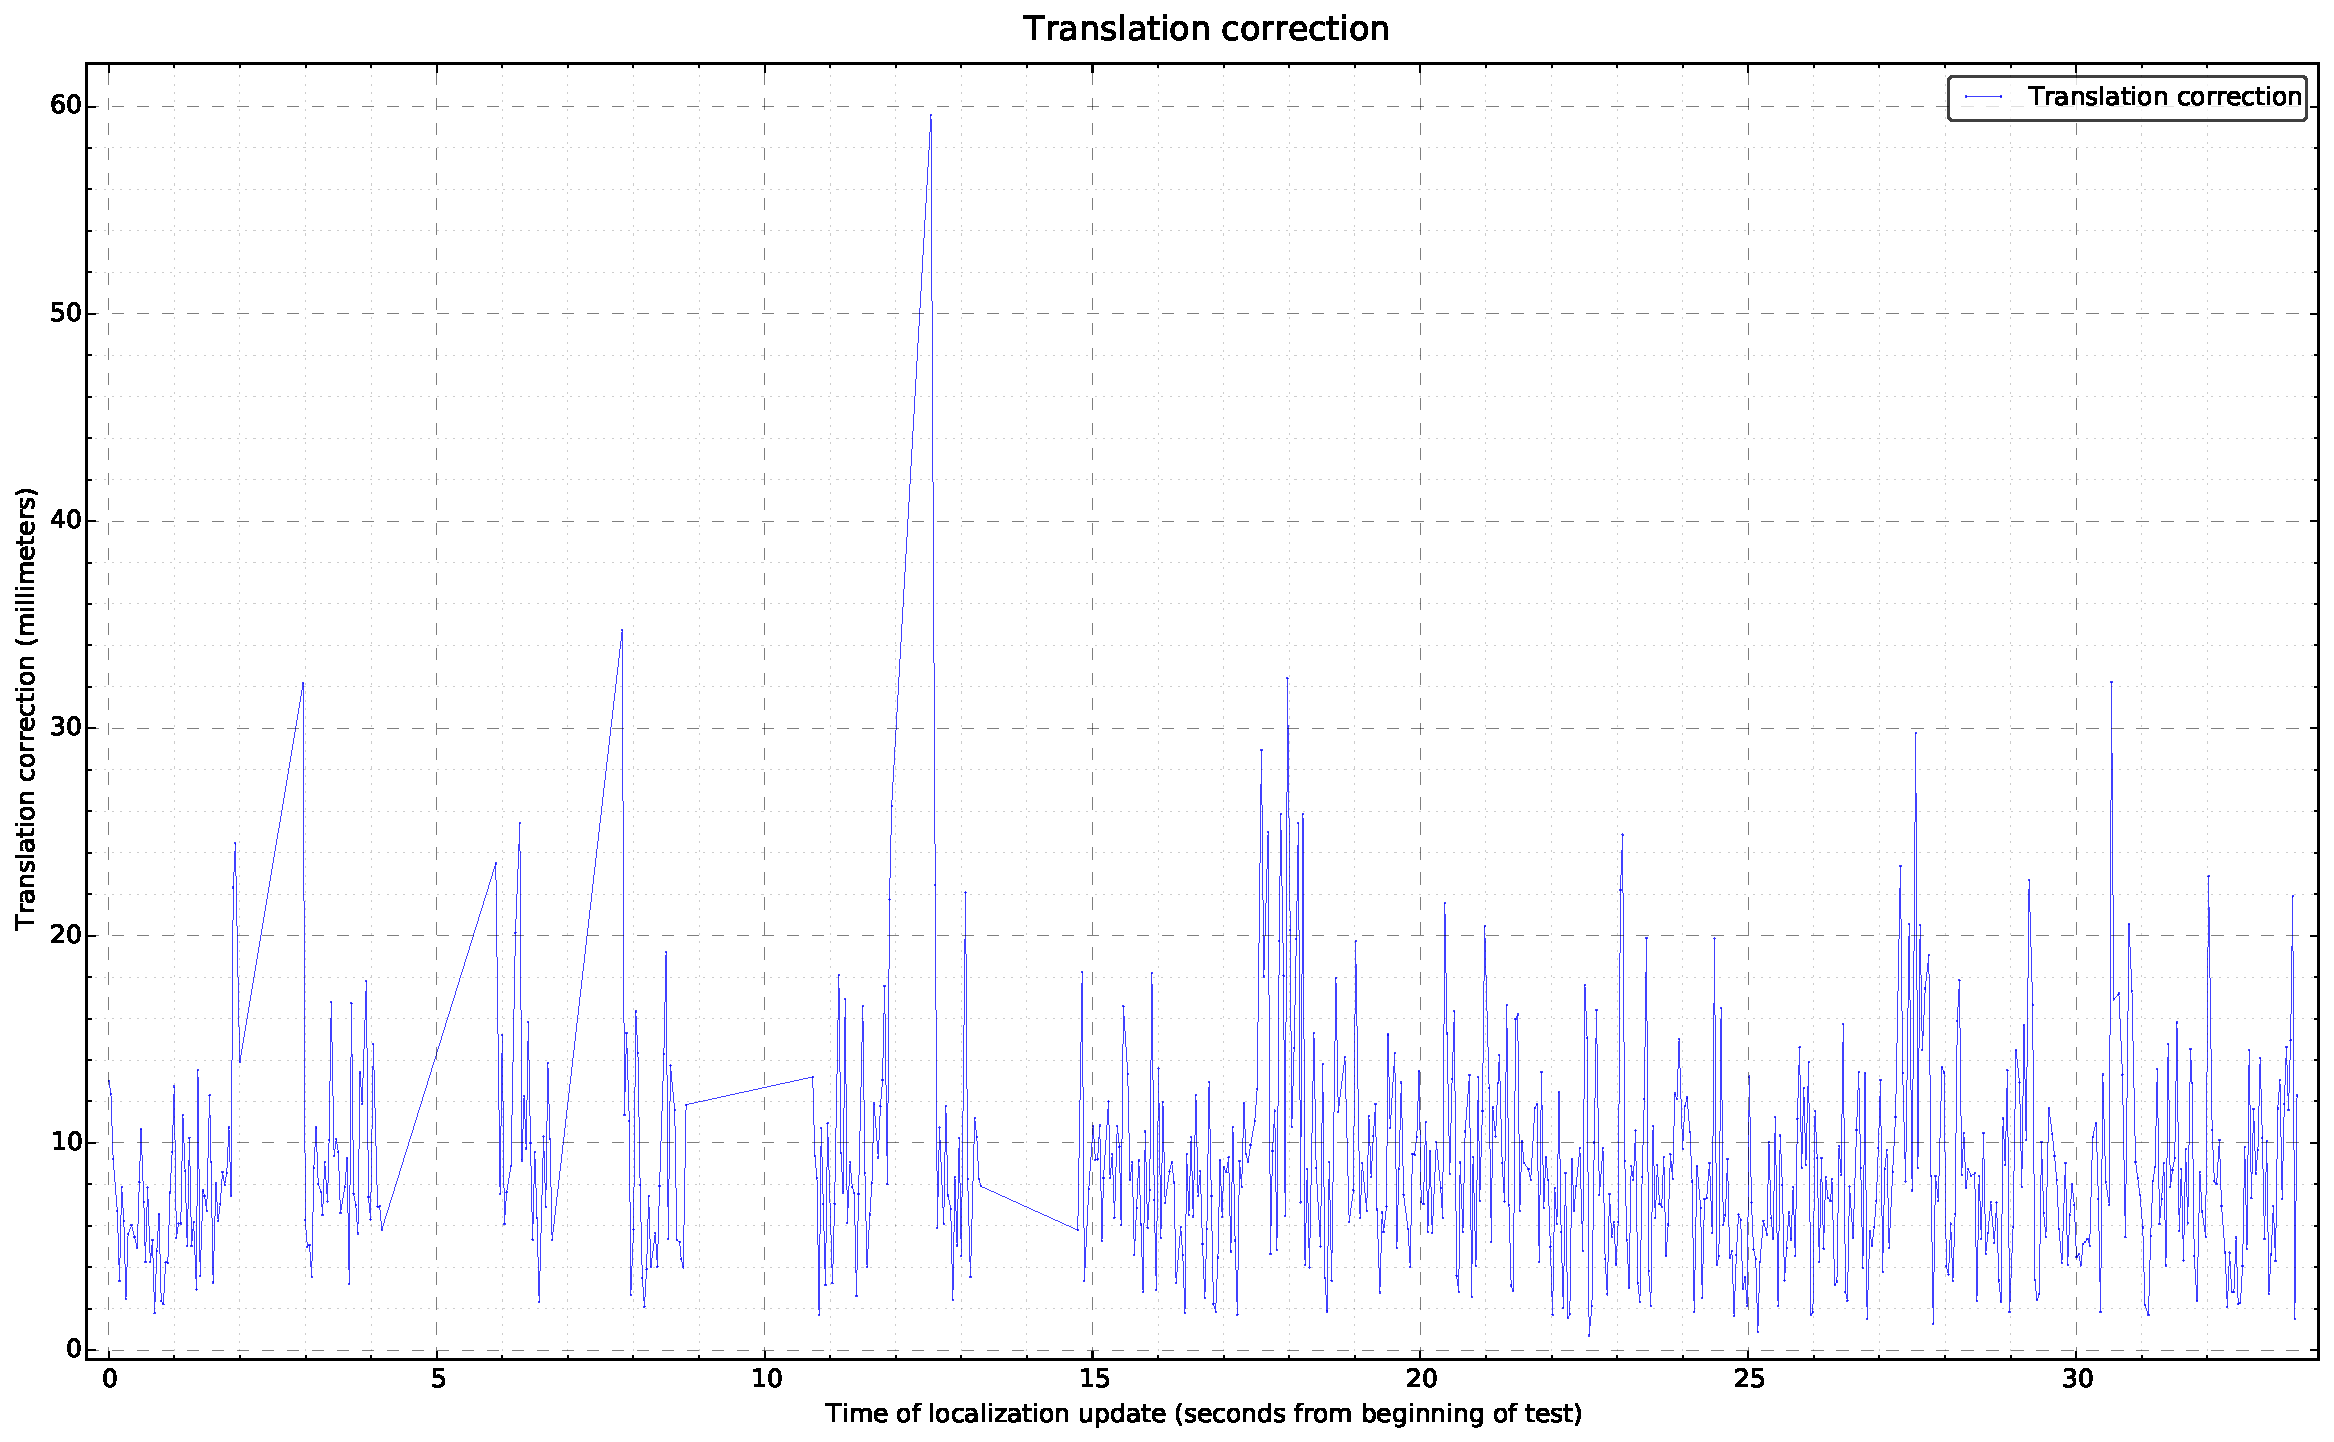
\includegraphics[width=0.69\textwidth]{appendices/tests-3dof/jarvis-robot/\currfilebase/graphs/translation-correction-millimeters}
	\caption{Translation corrections performed by the localization system}
\end{figure}

\begin{figure}[H]
	\centering
	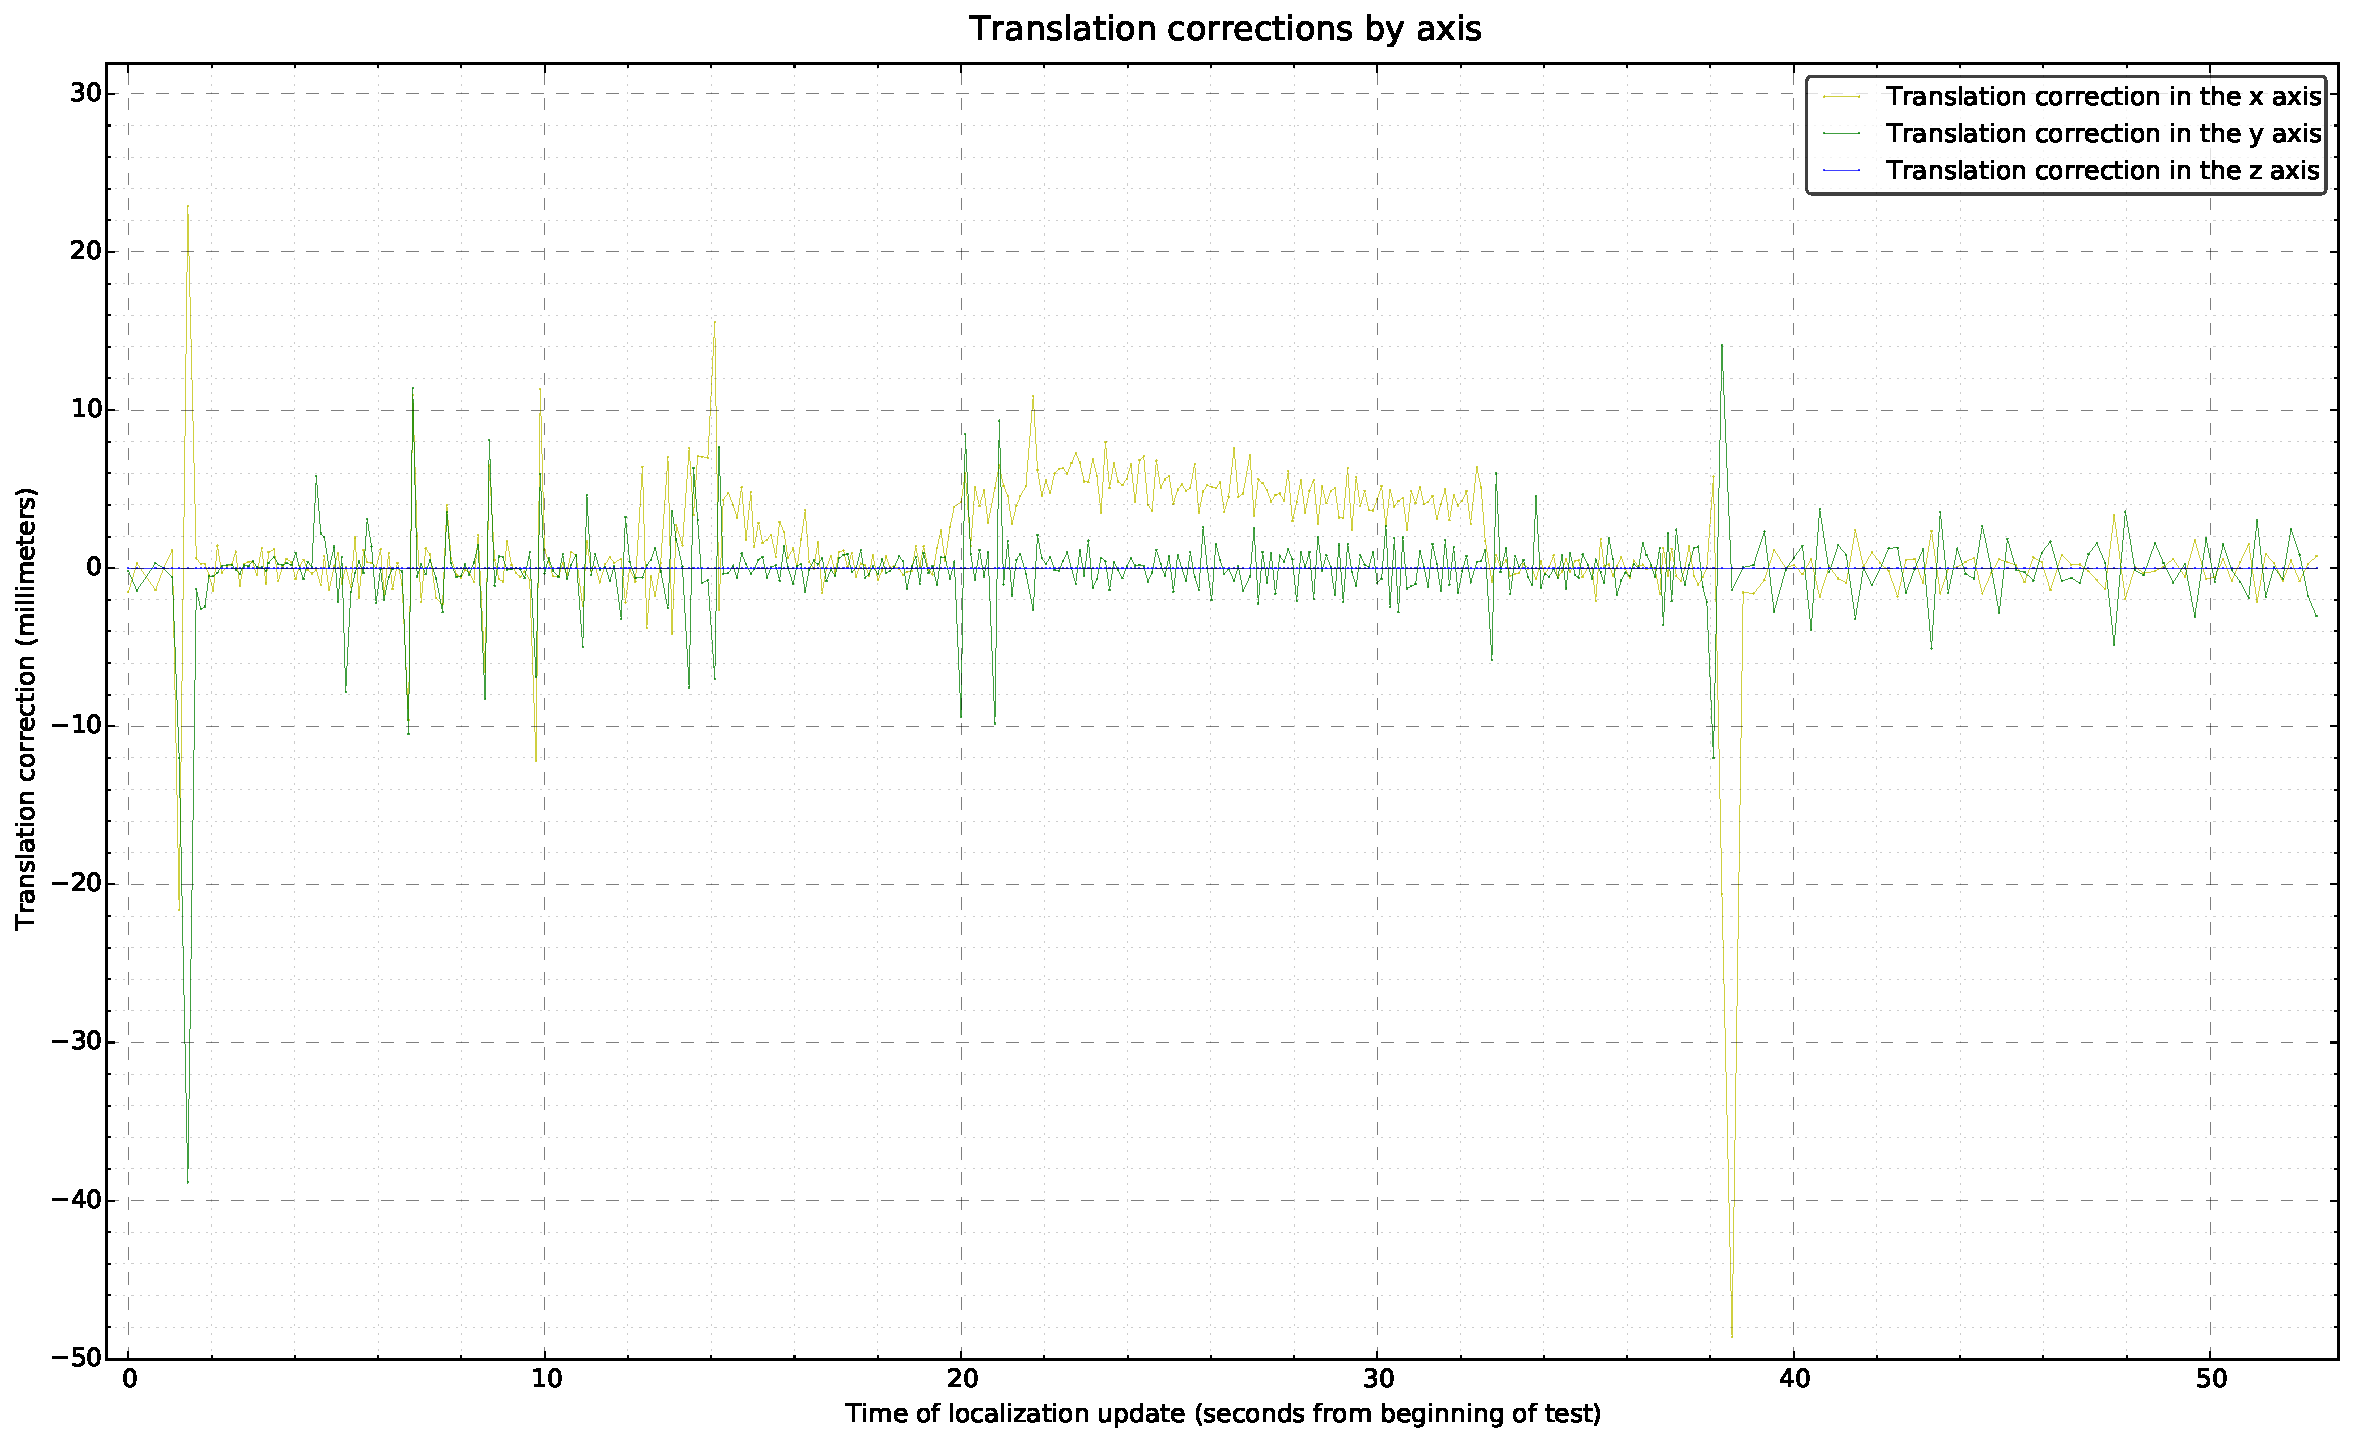
\includegraphics[width=0.69\textwidth]{appendices/tests-3dof/jarvis-robot/\currfilebase/graphs/translation-corrections-components-millimeters}
	\caption{Translation corrections components performed by the localization system}
\end{figure}

\begin{figure}[H]
	\centering
	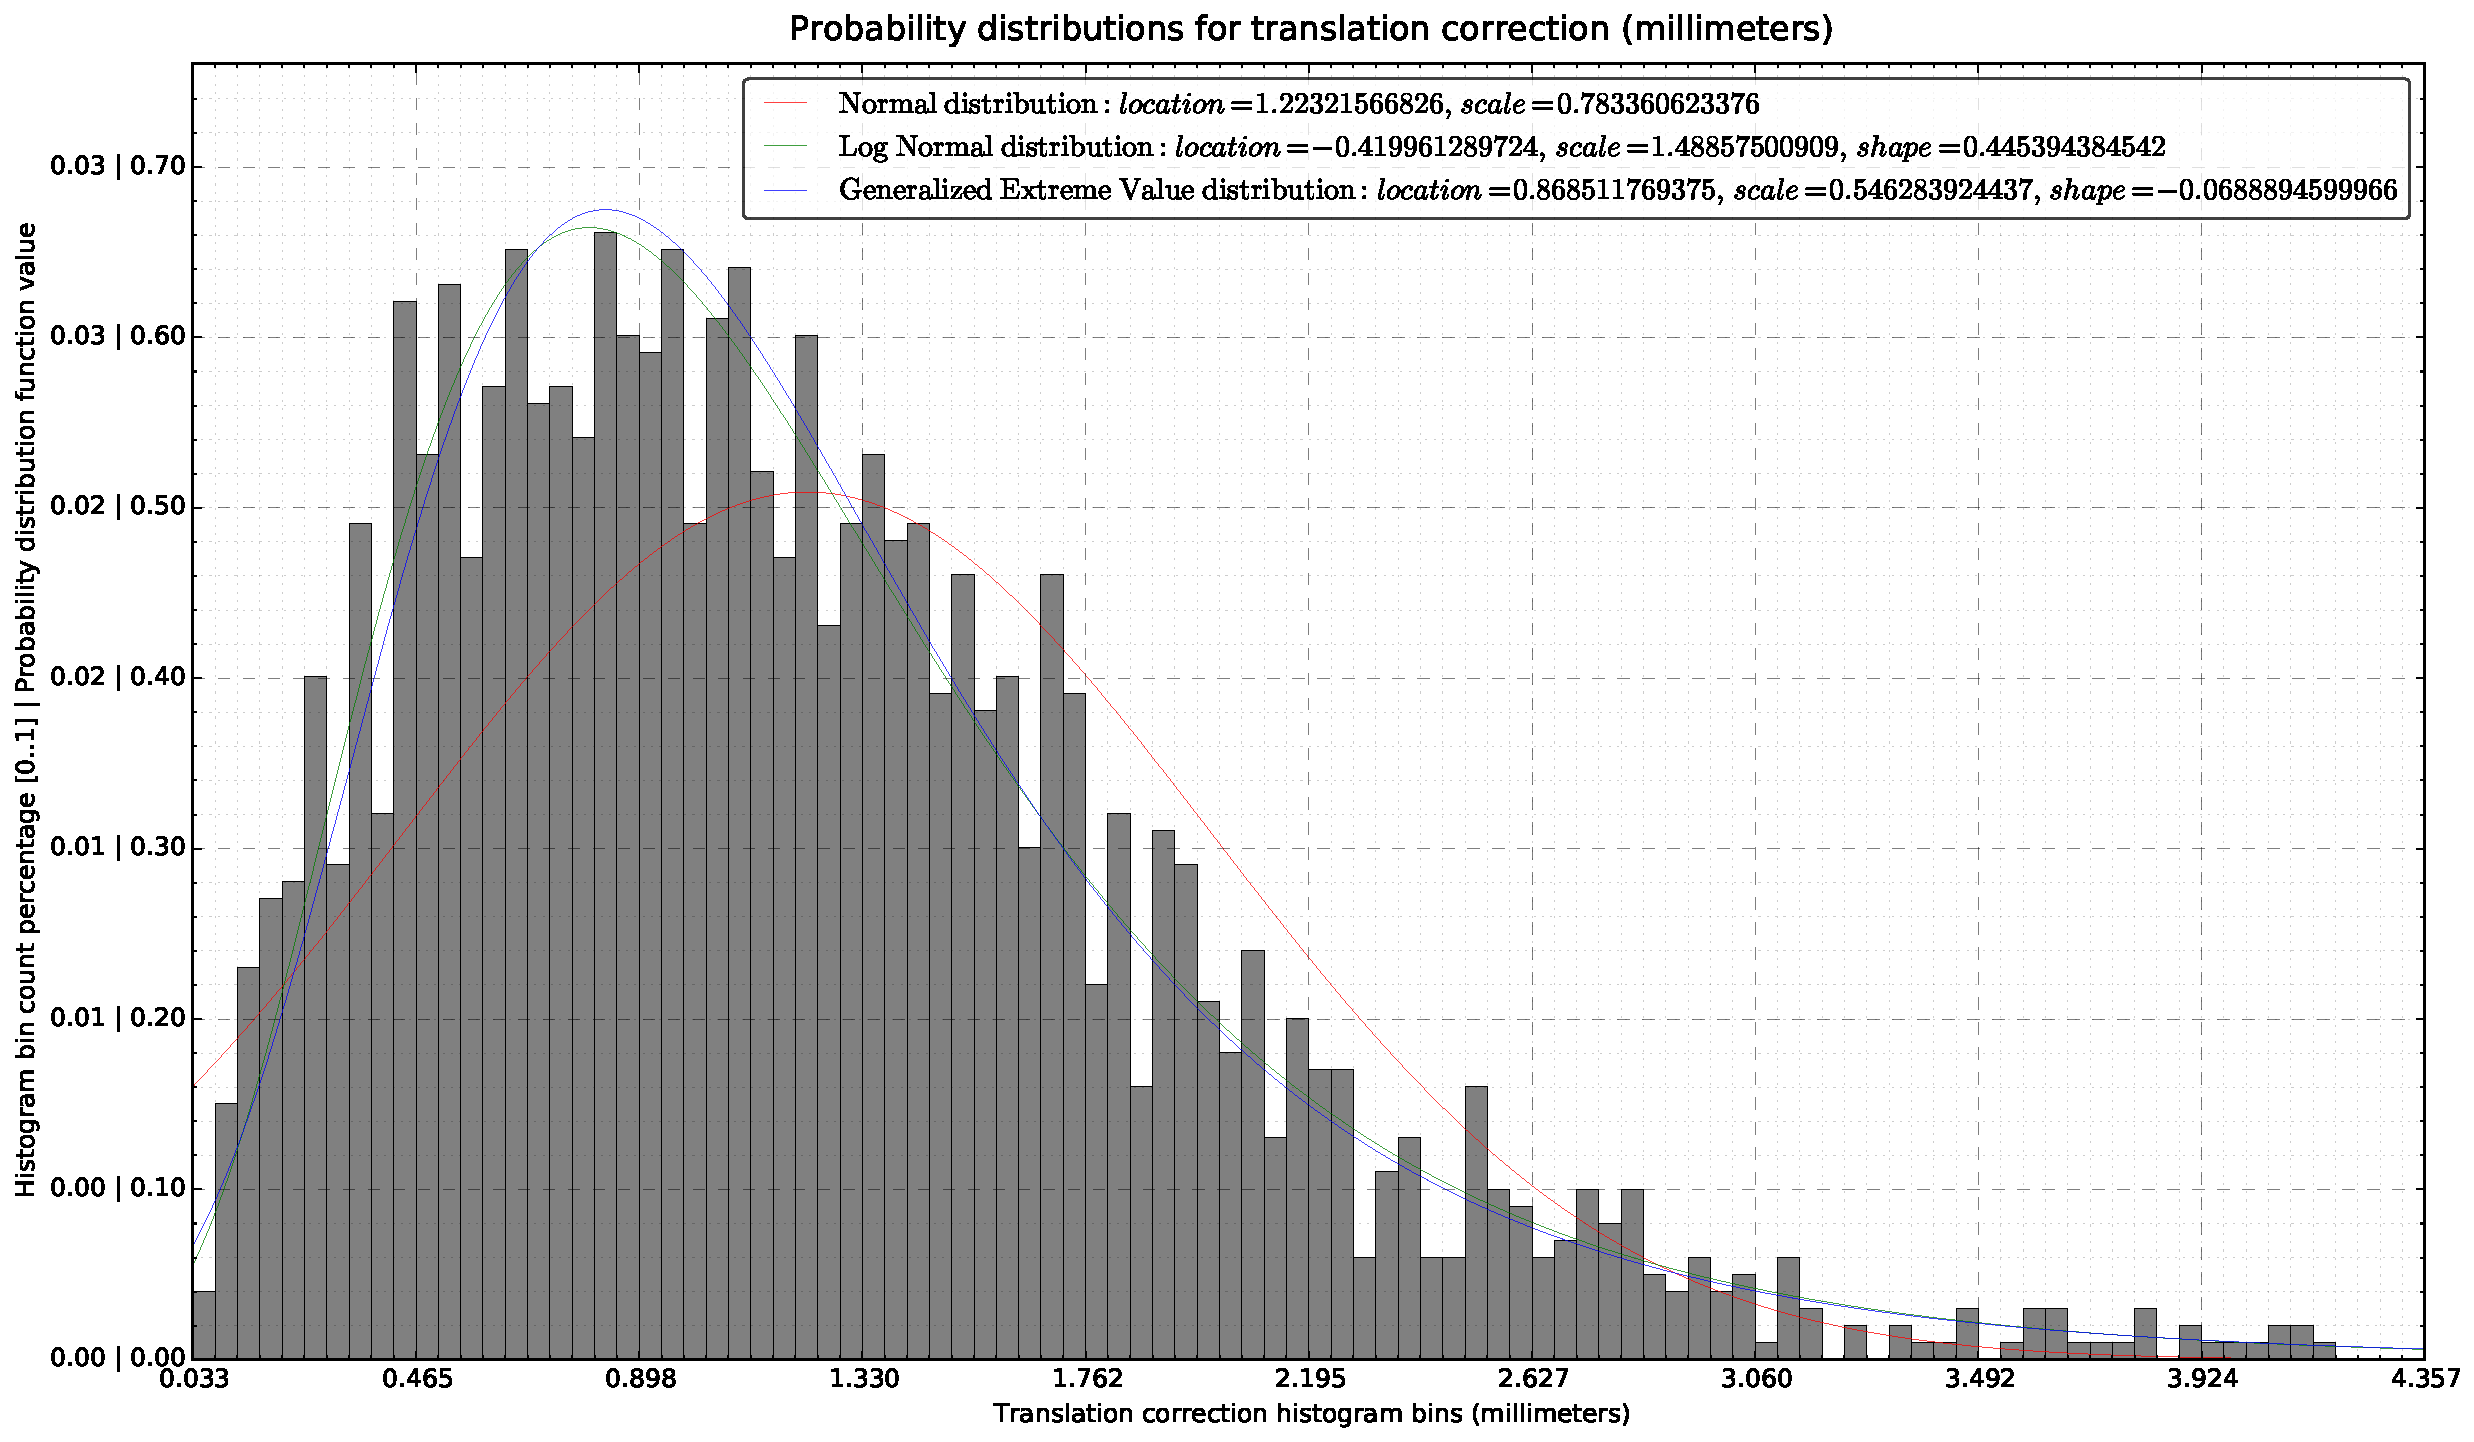
\includegraphics[width=0.69\textwidth]{appendices/tests-3dof/jarvis-robot/\currfilebase/graphs/translation-correction-millimeters-distributions}
	\caption{Probability distributions for the translation corrections performed by the localization system}
\end{figure}


%Rotation corrections axis
\begin{figure}[H]
	\centering
	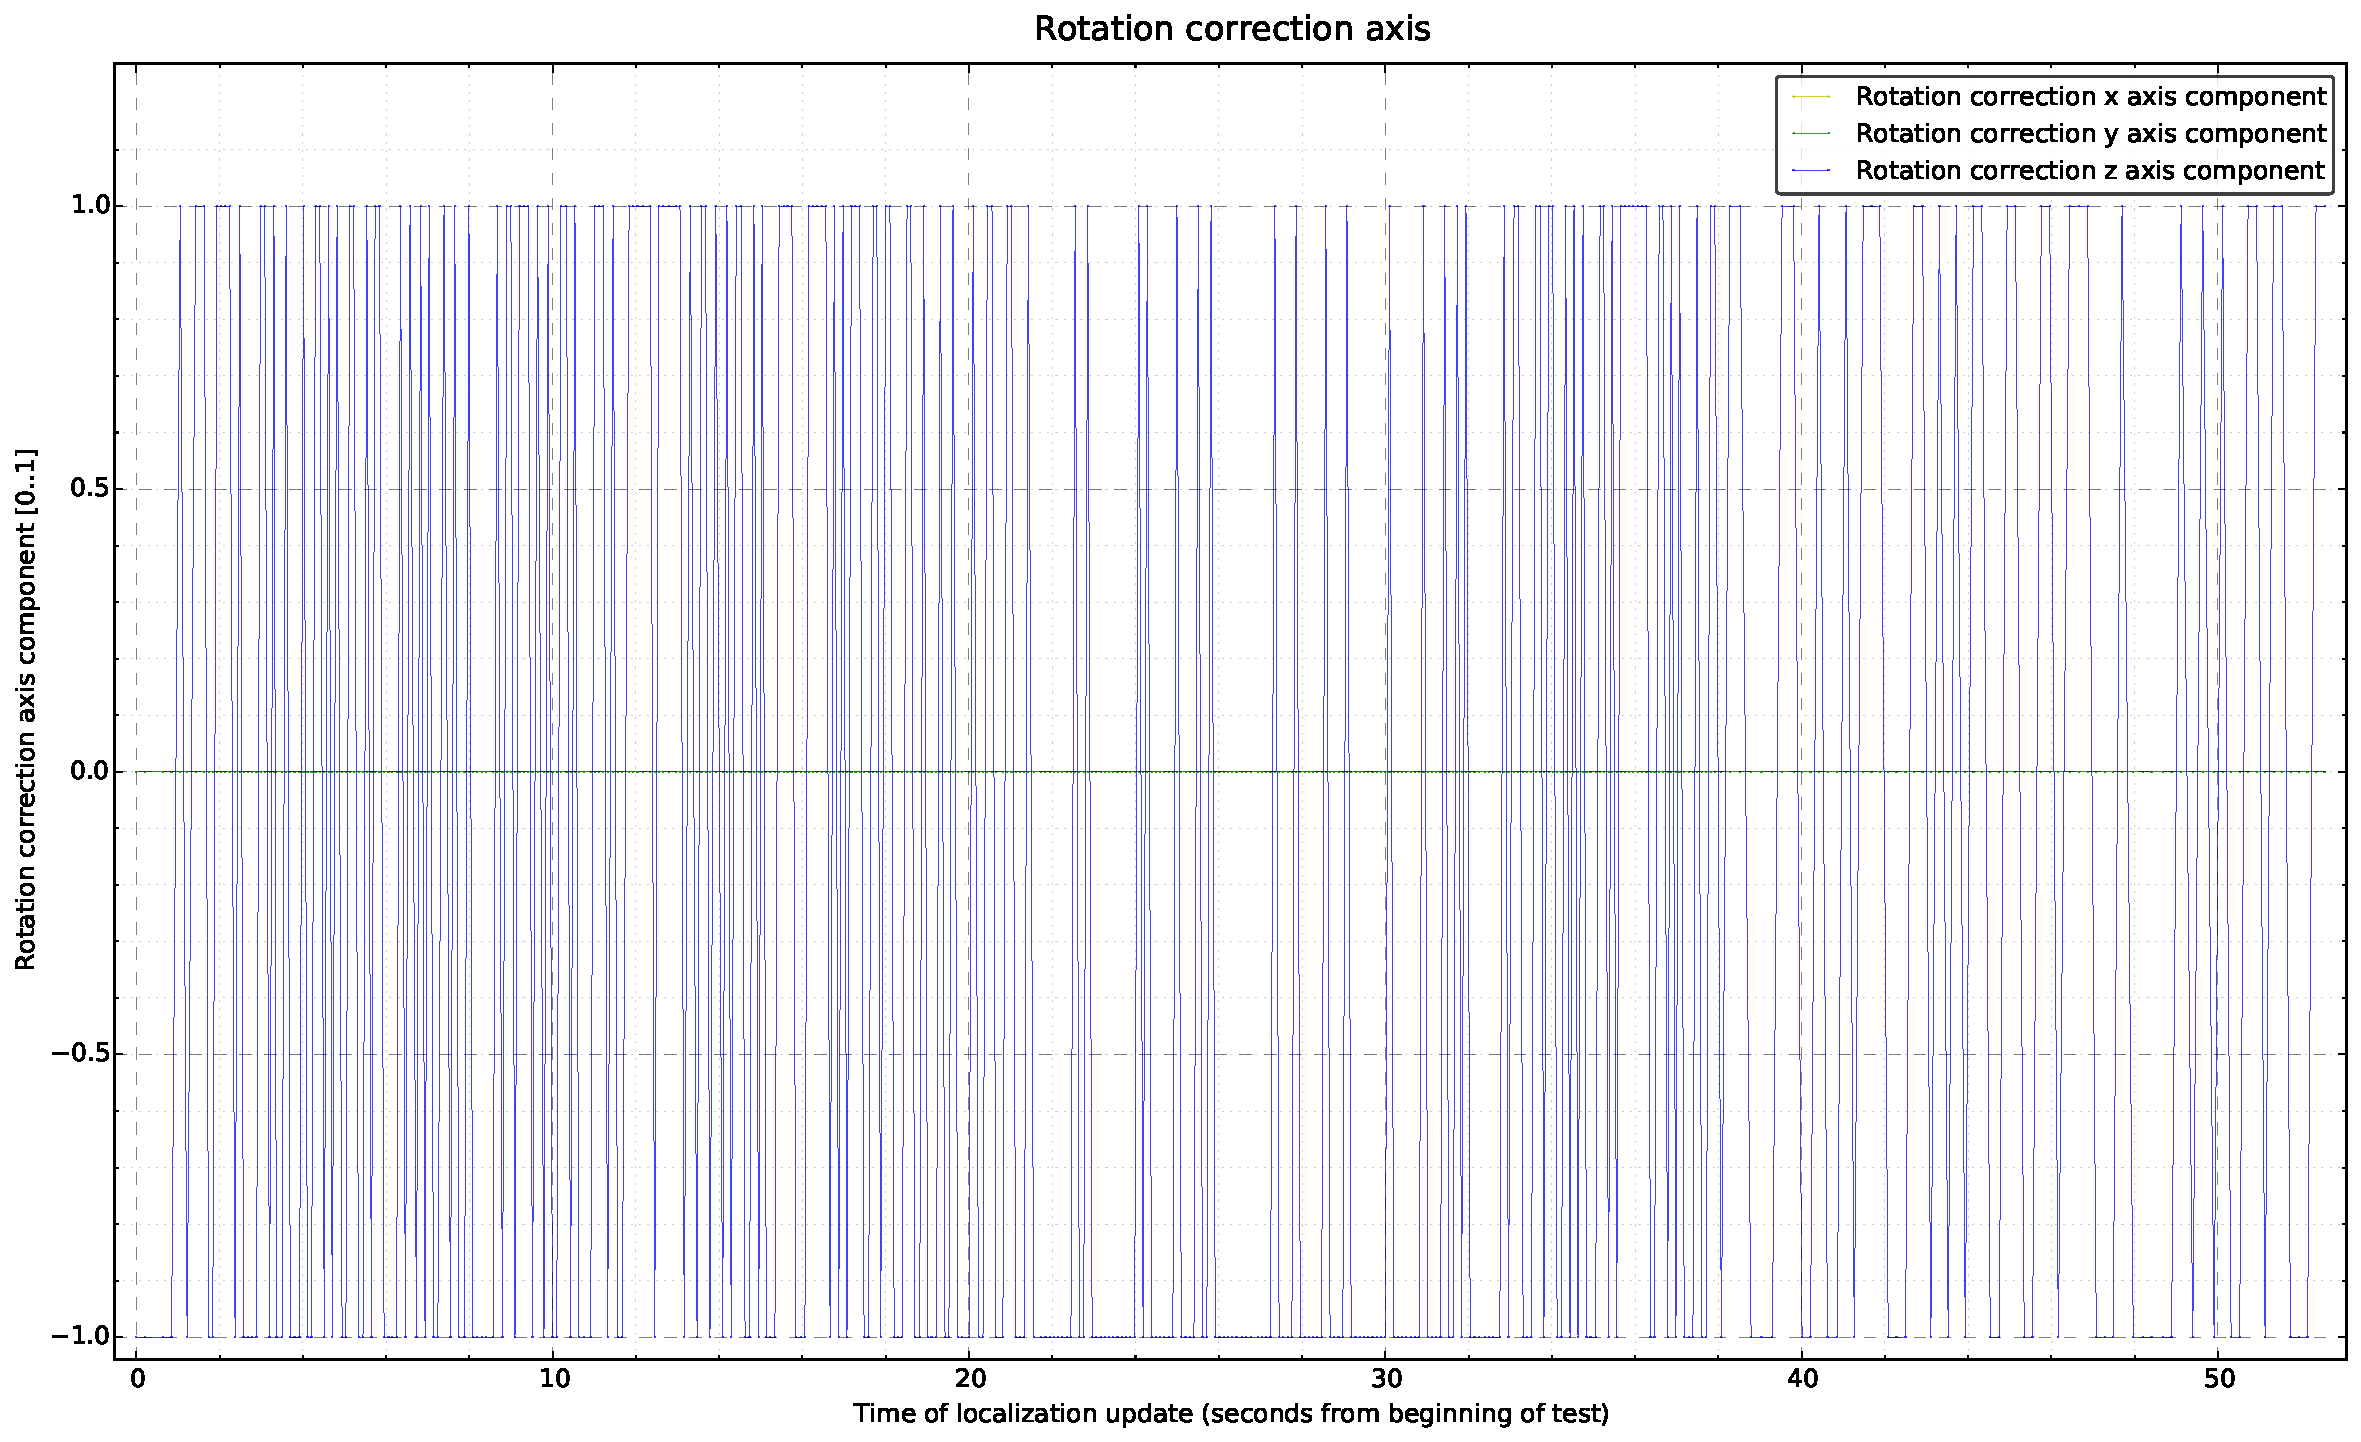
\includegraphics[width=0.69\textwidth]{appendices/tests-3dof/jarvis-robot/\currfilebase/graphs/rotation-correction-axis}
	\caption{Rotation corrections (axis) performed by the localization system}
\end{figure}

\begin{figure}[H]
	\centering
	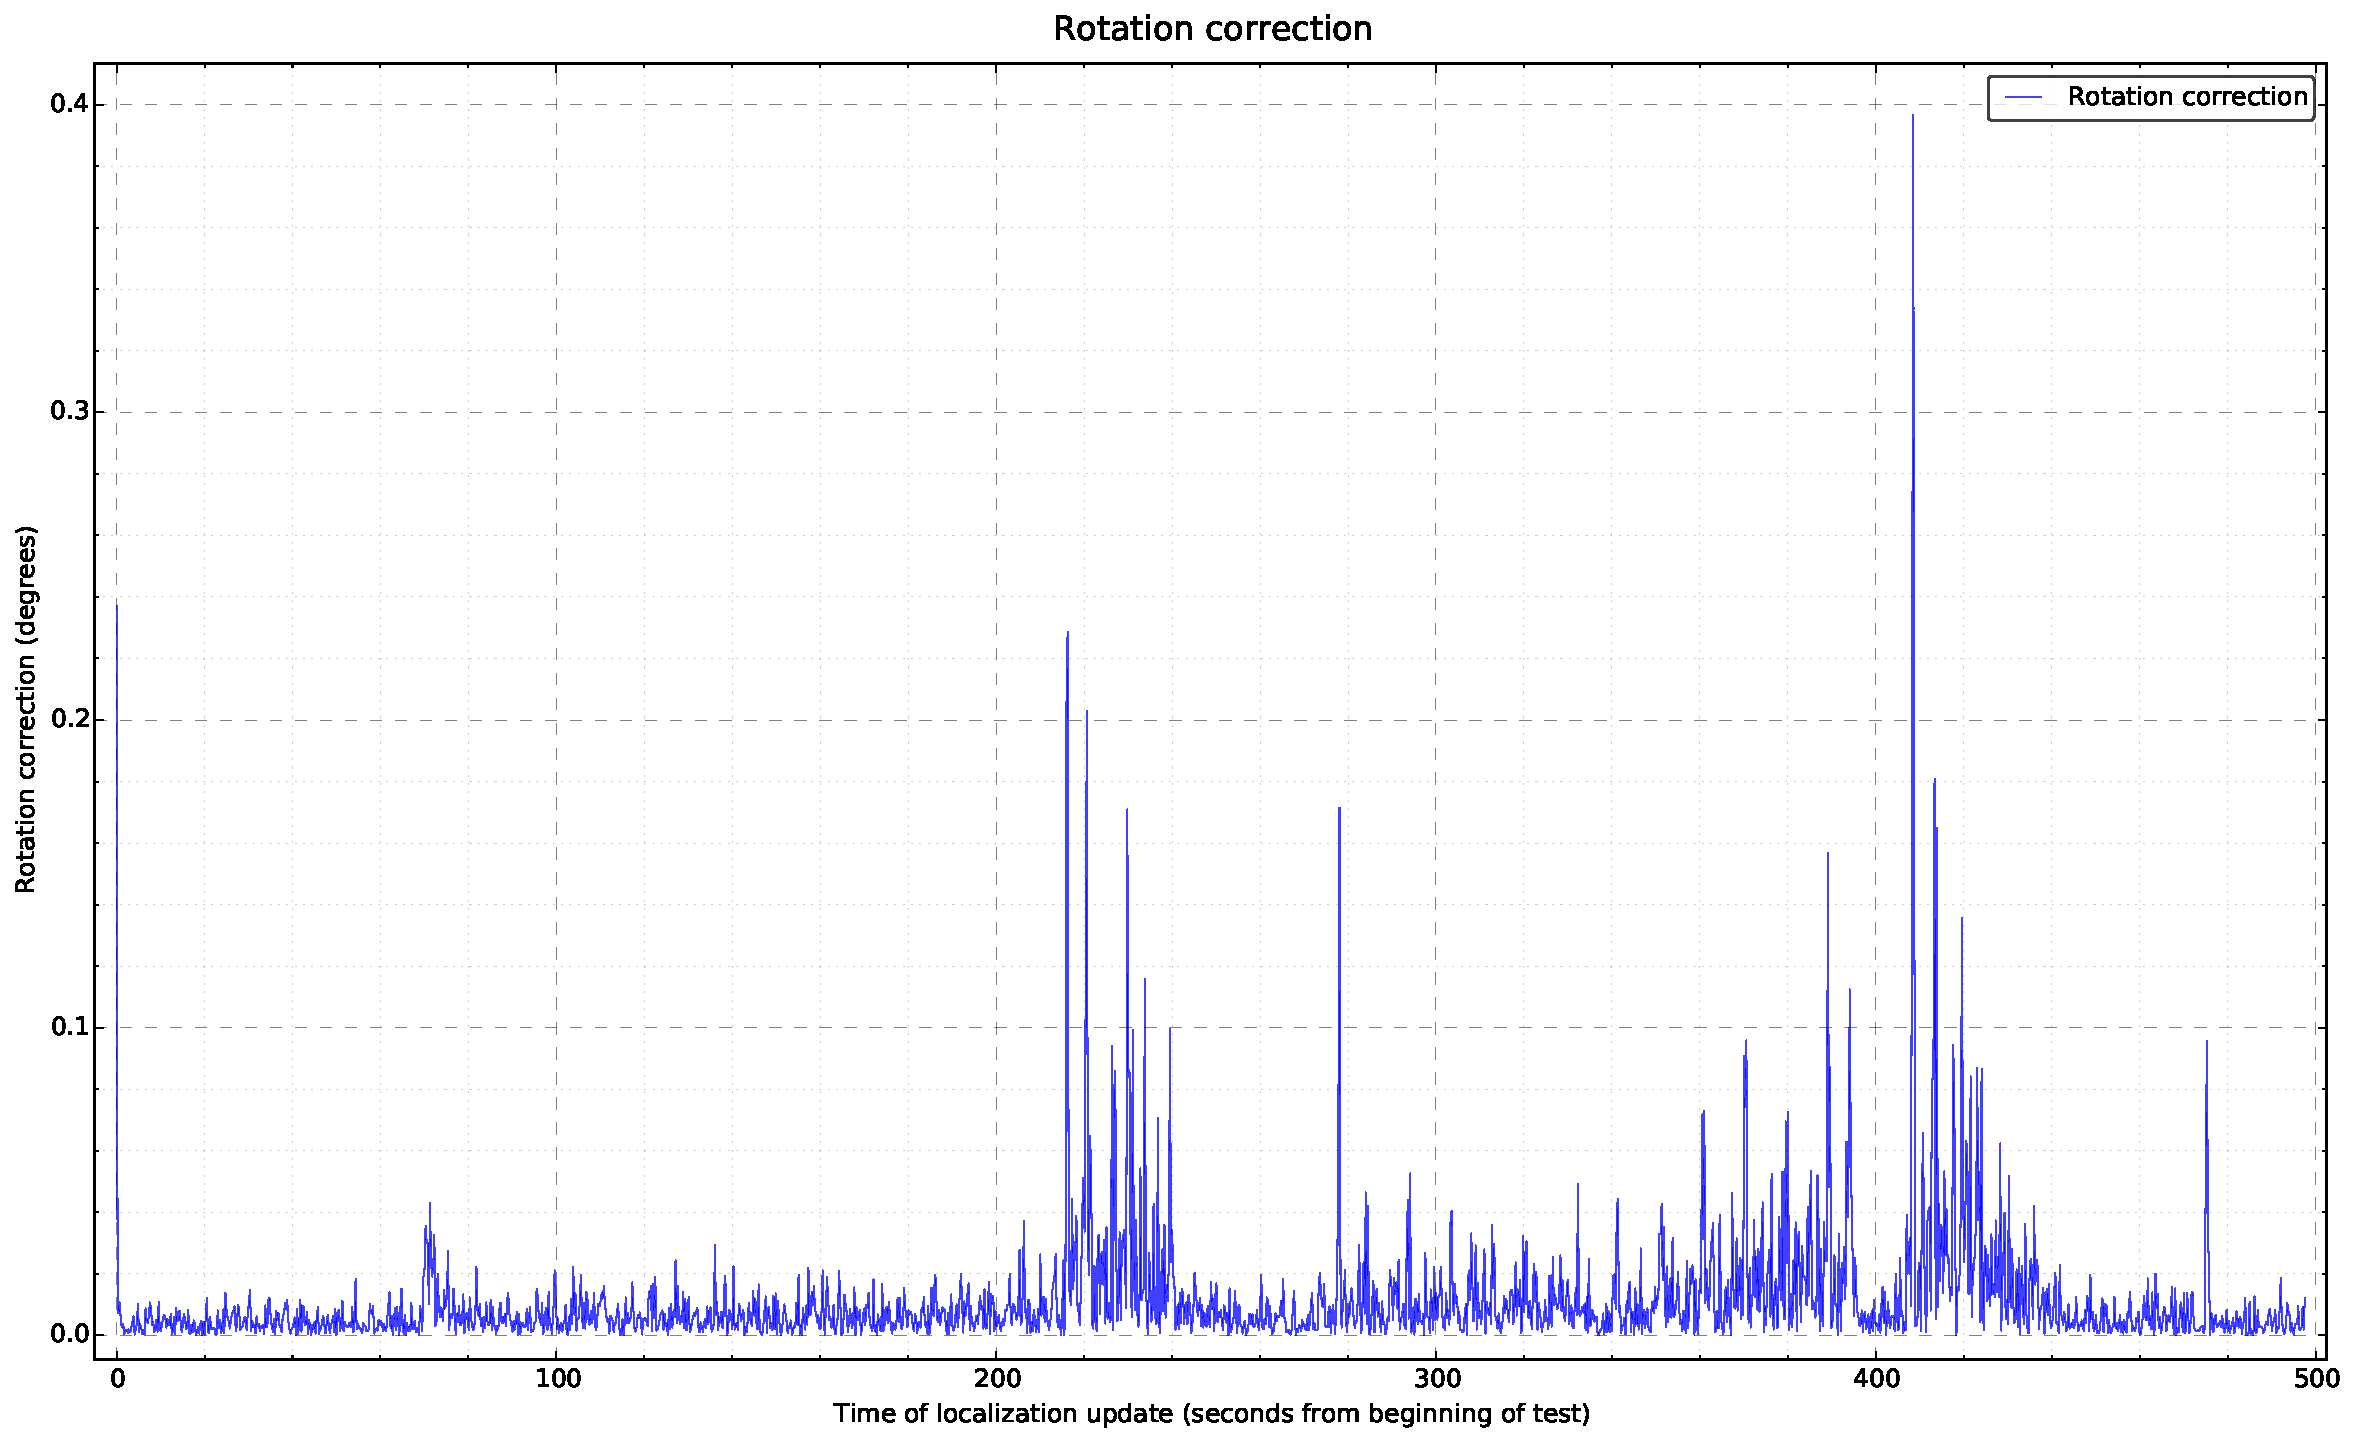
\includegraphics[width=0.69\textwidth]{appendices/tests-3dof/jarvis-robot/\currfilebase/graphs/rotation-correction-degrees}
	\caption{Rotation corrections performed by the localization system}
\end{figure}

\begin{figure}[H]
	\centering
	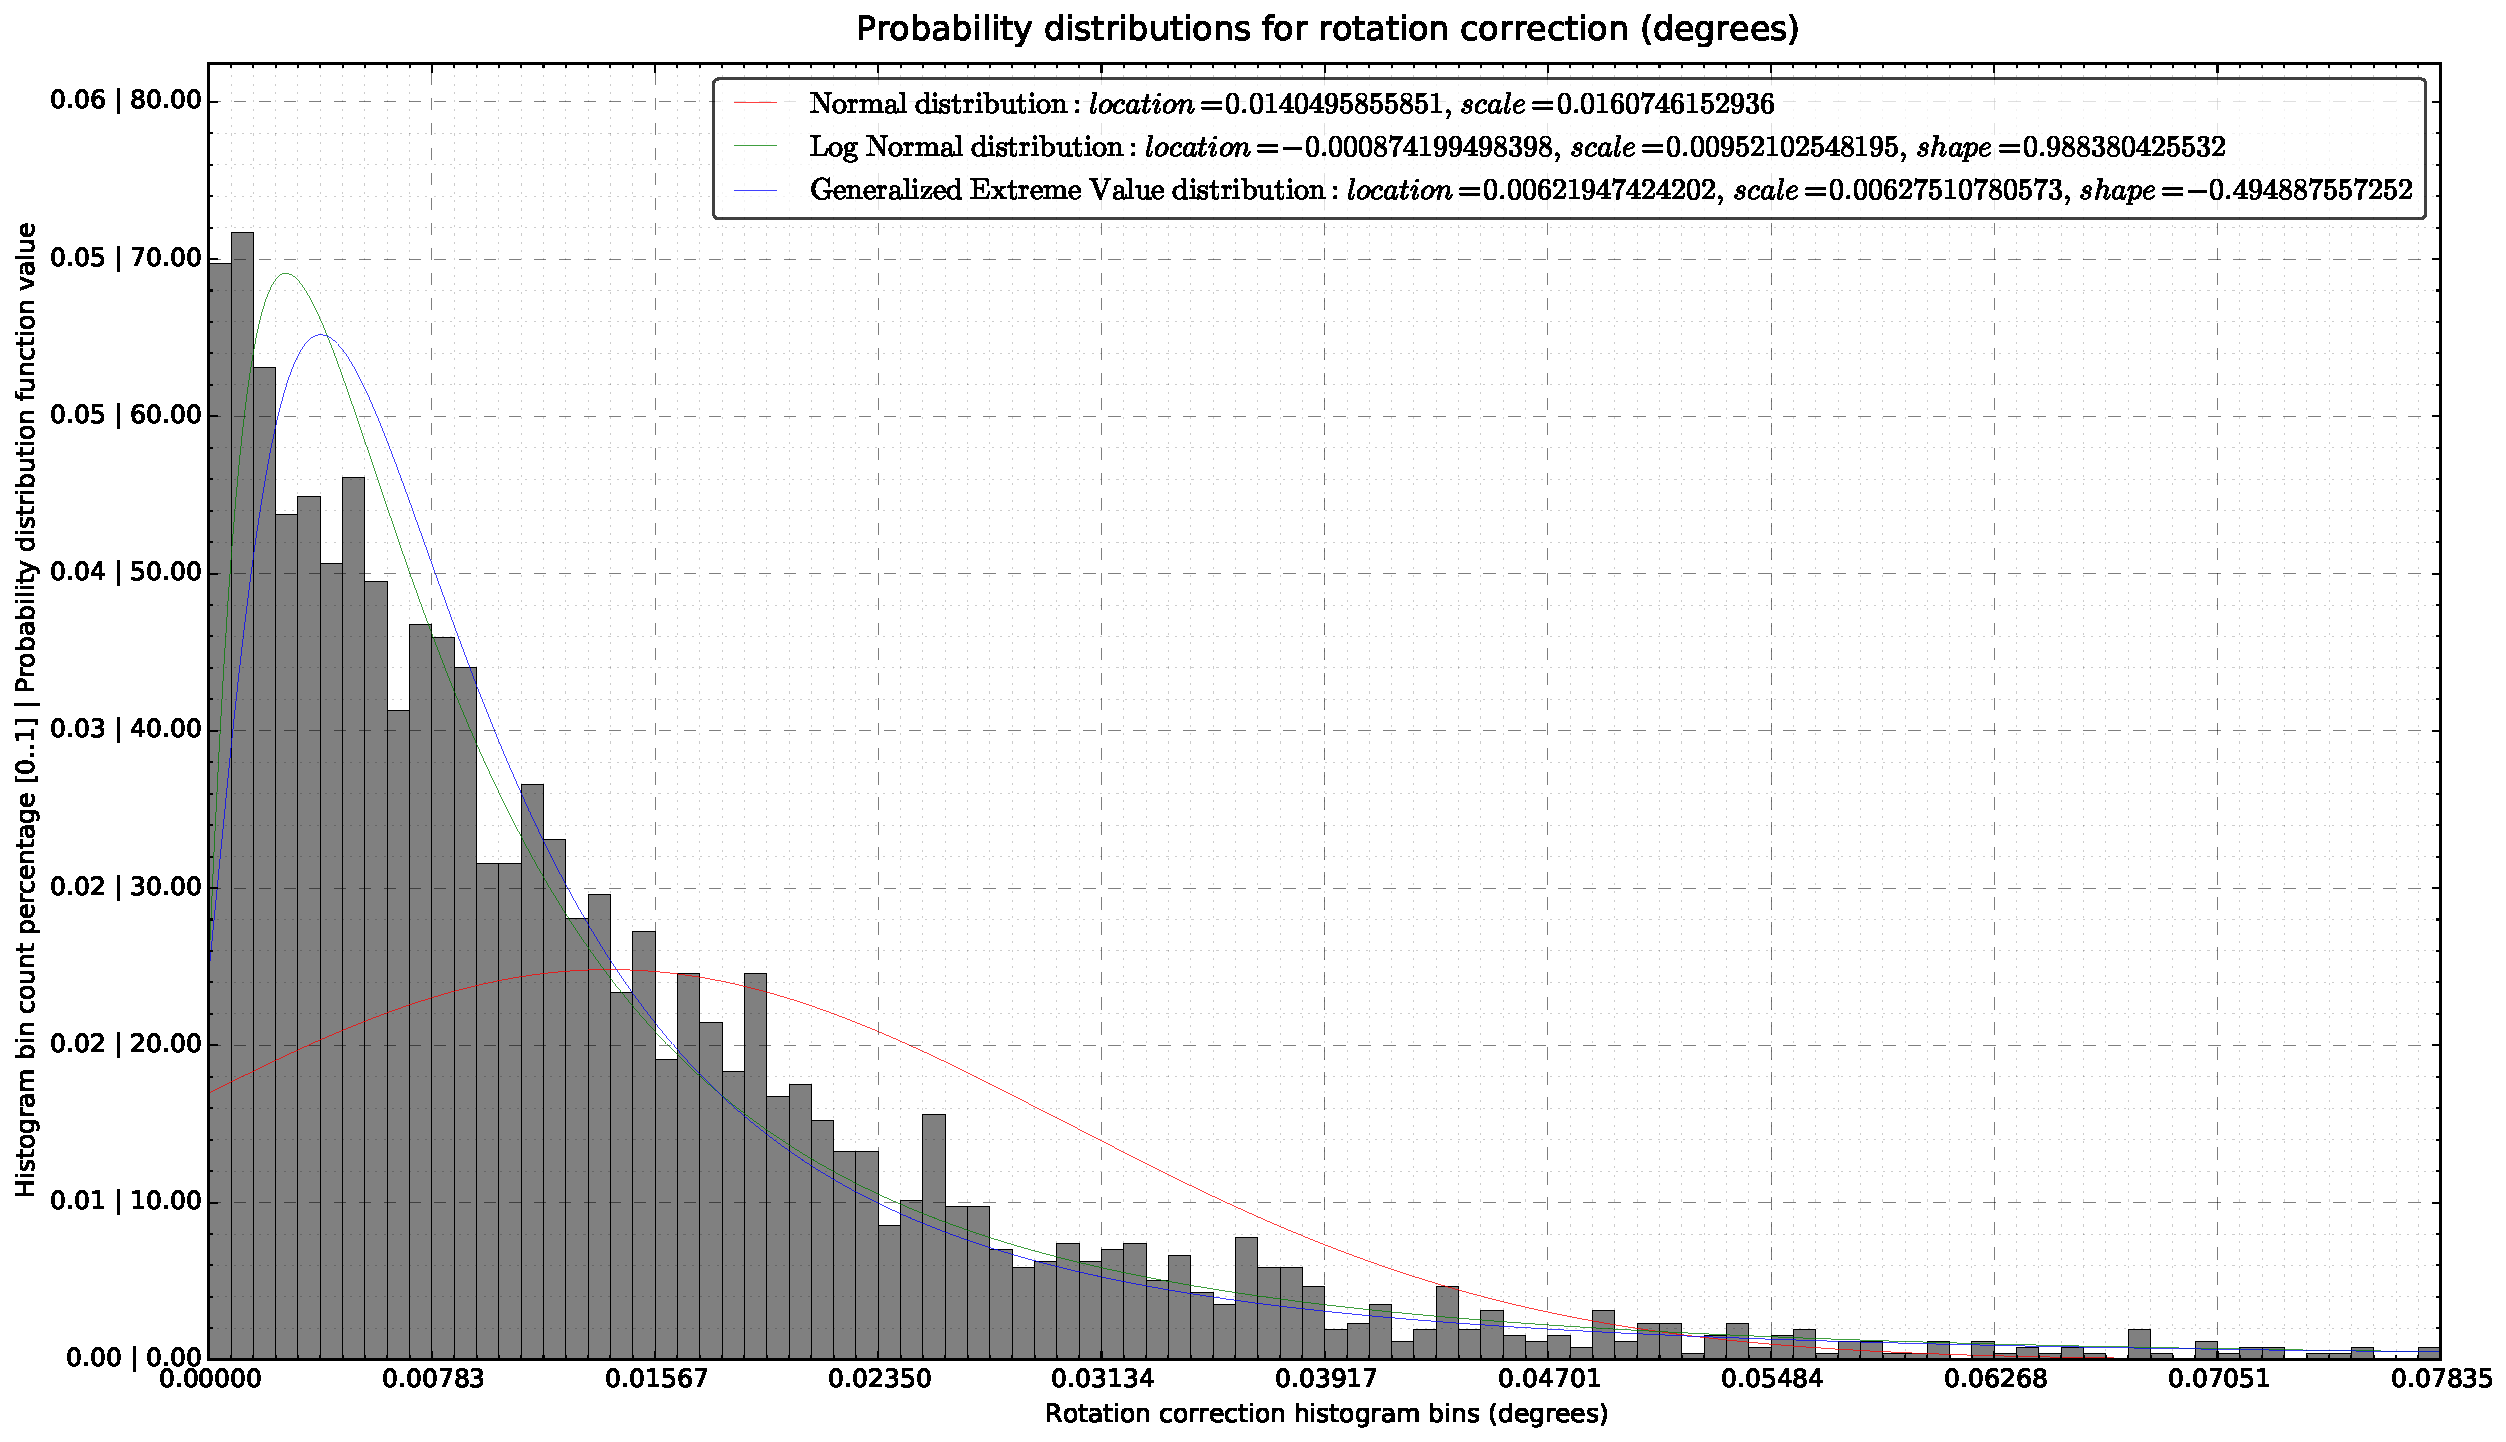
\includegraphics[width=0.69\textwidth]{appendices/tests-3dof/jarvis-robot/\currfilebase/graphs/rotation-correction-degrees-distributions}
	\caption{Probability distributions for the rotation corrections performed by the localization system}
\end{figure}


%Registered points (inliers / outliers)
\begin{figure}[H]
	\centering
	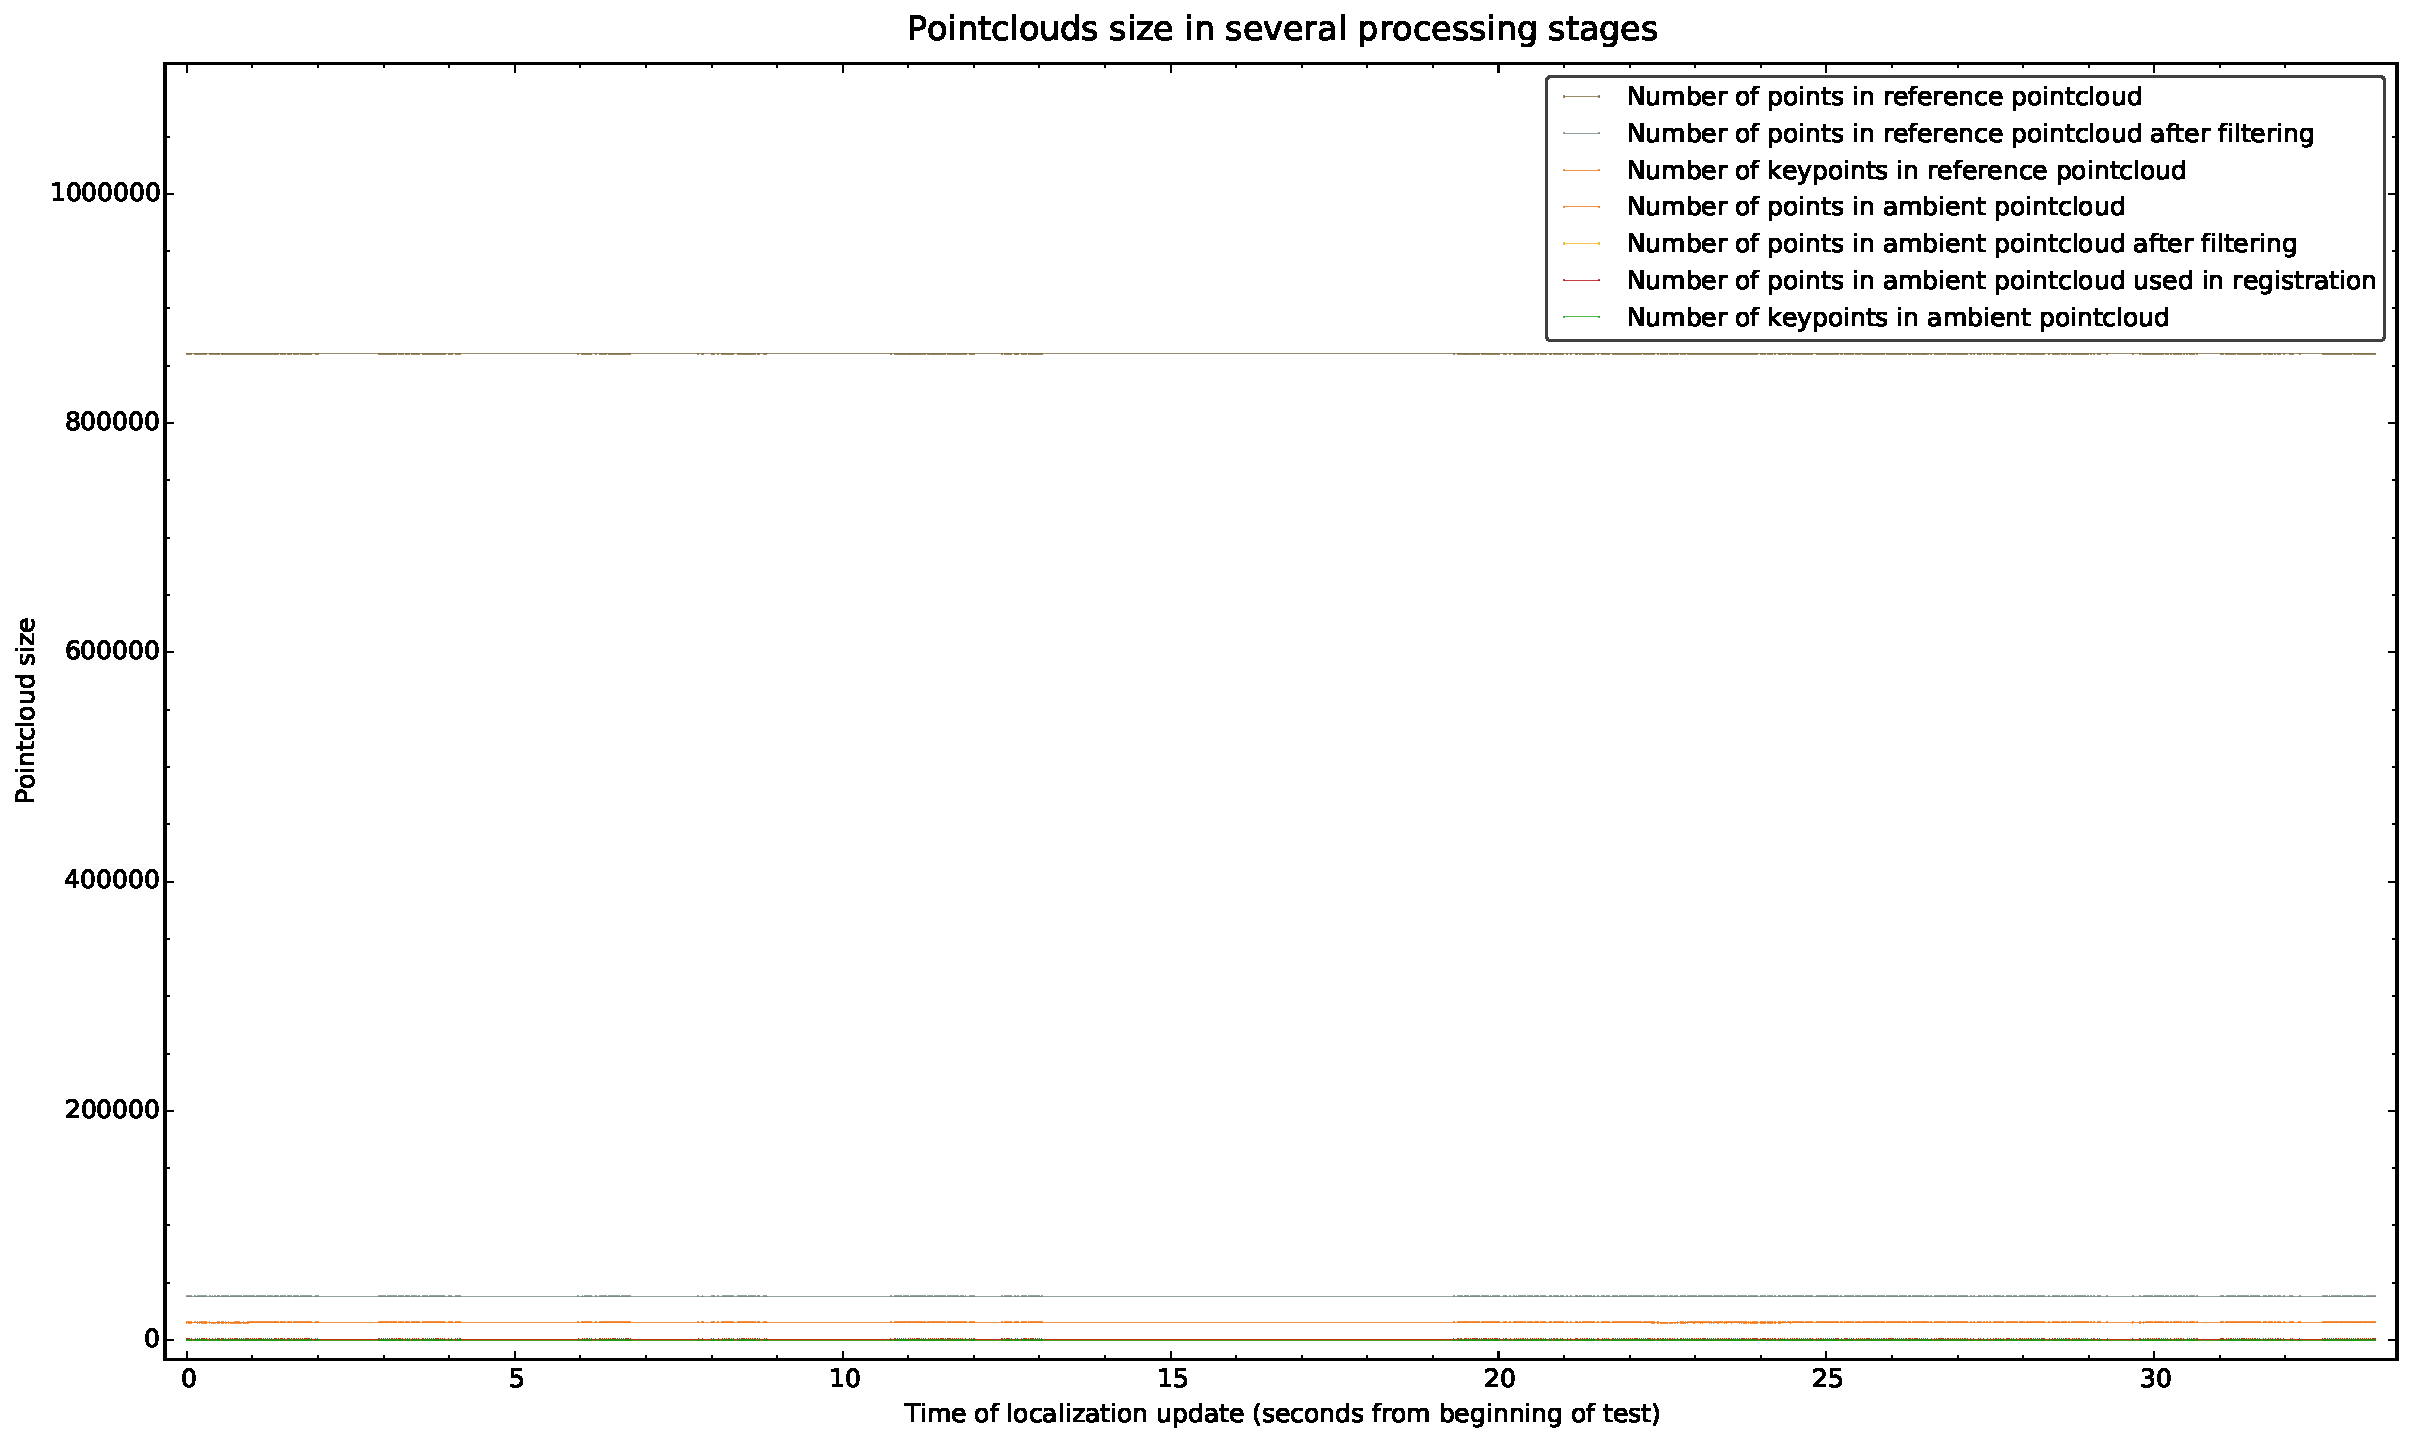
\includegraphics[width=0.69\textwidth]{appendices/tests-3dof/jarvis-robot/\currfilebase/graphs/pointclouds-size}
	\caption{Point clouds size in several of the localization system processing stages}
\end{figure}

\begin{figure}[H]
	\centering
	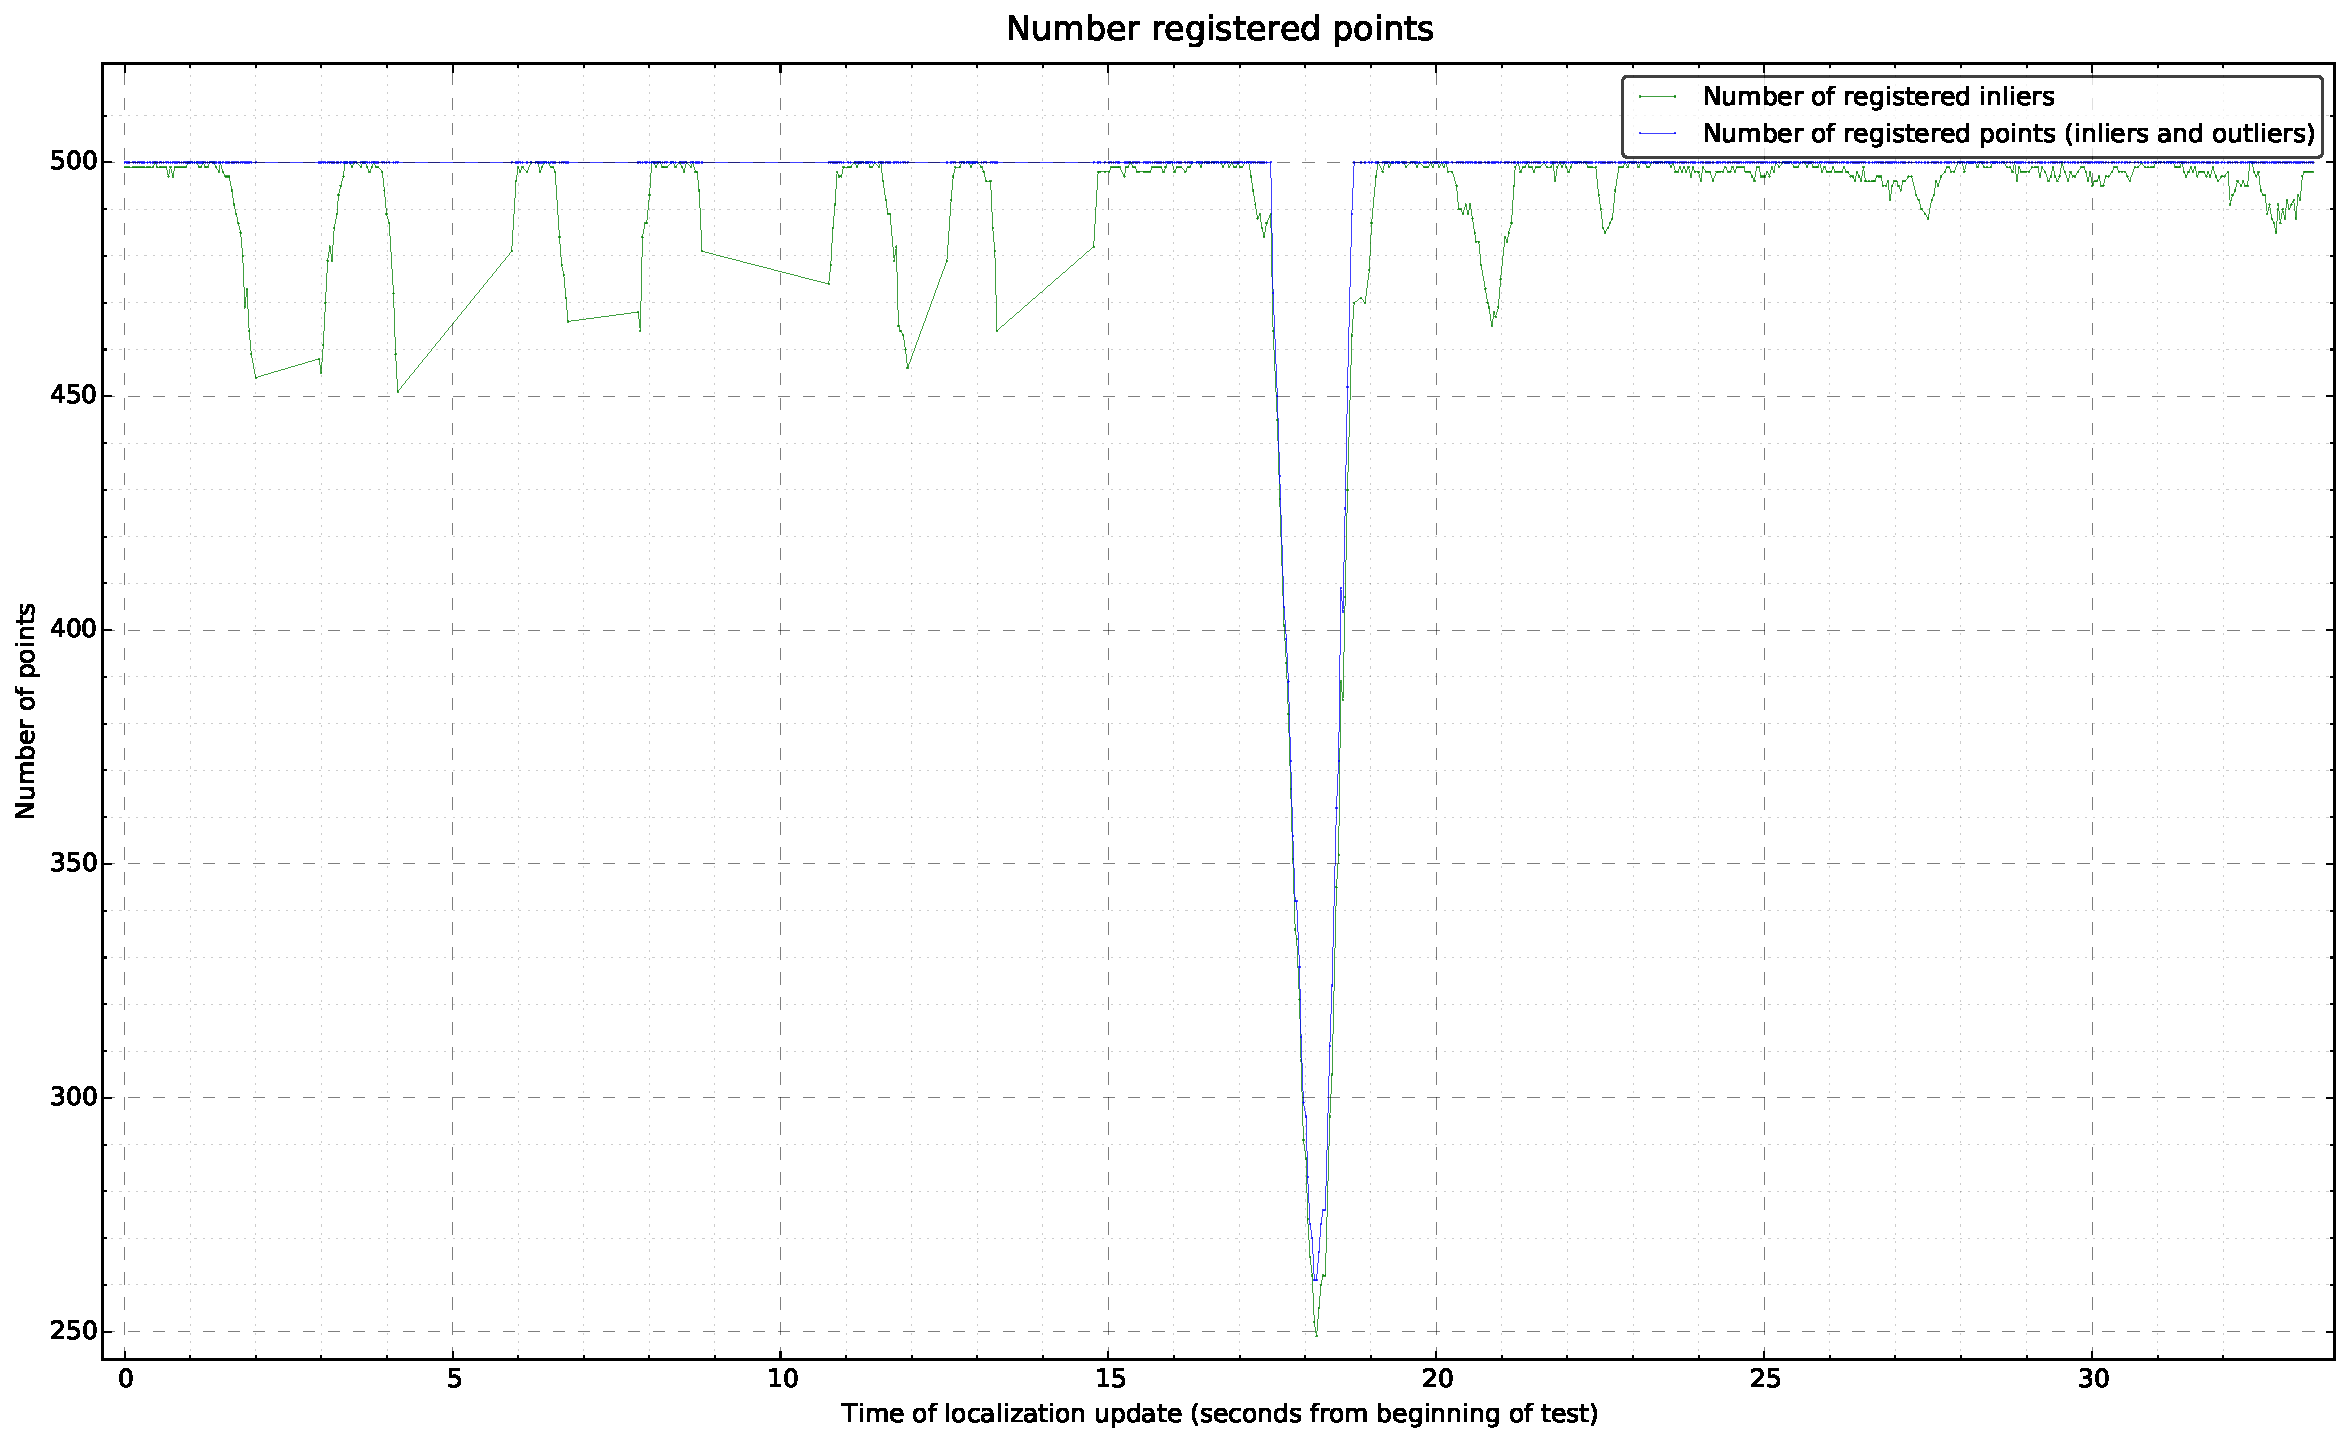
\includegraphics[width=0.69\textwidth]{appendices/tests-3dof/jarvis-robot/\currfilebase/graphs/registered-points}
	\caption{Number of registered points}
\end{figure}

\begin{figure}[H]
	\centering
	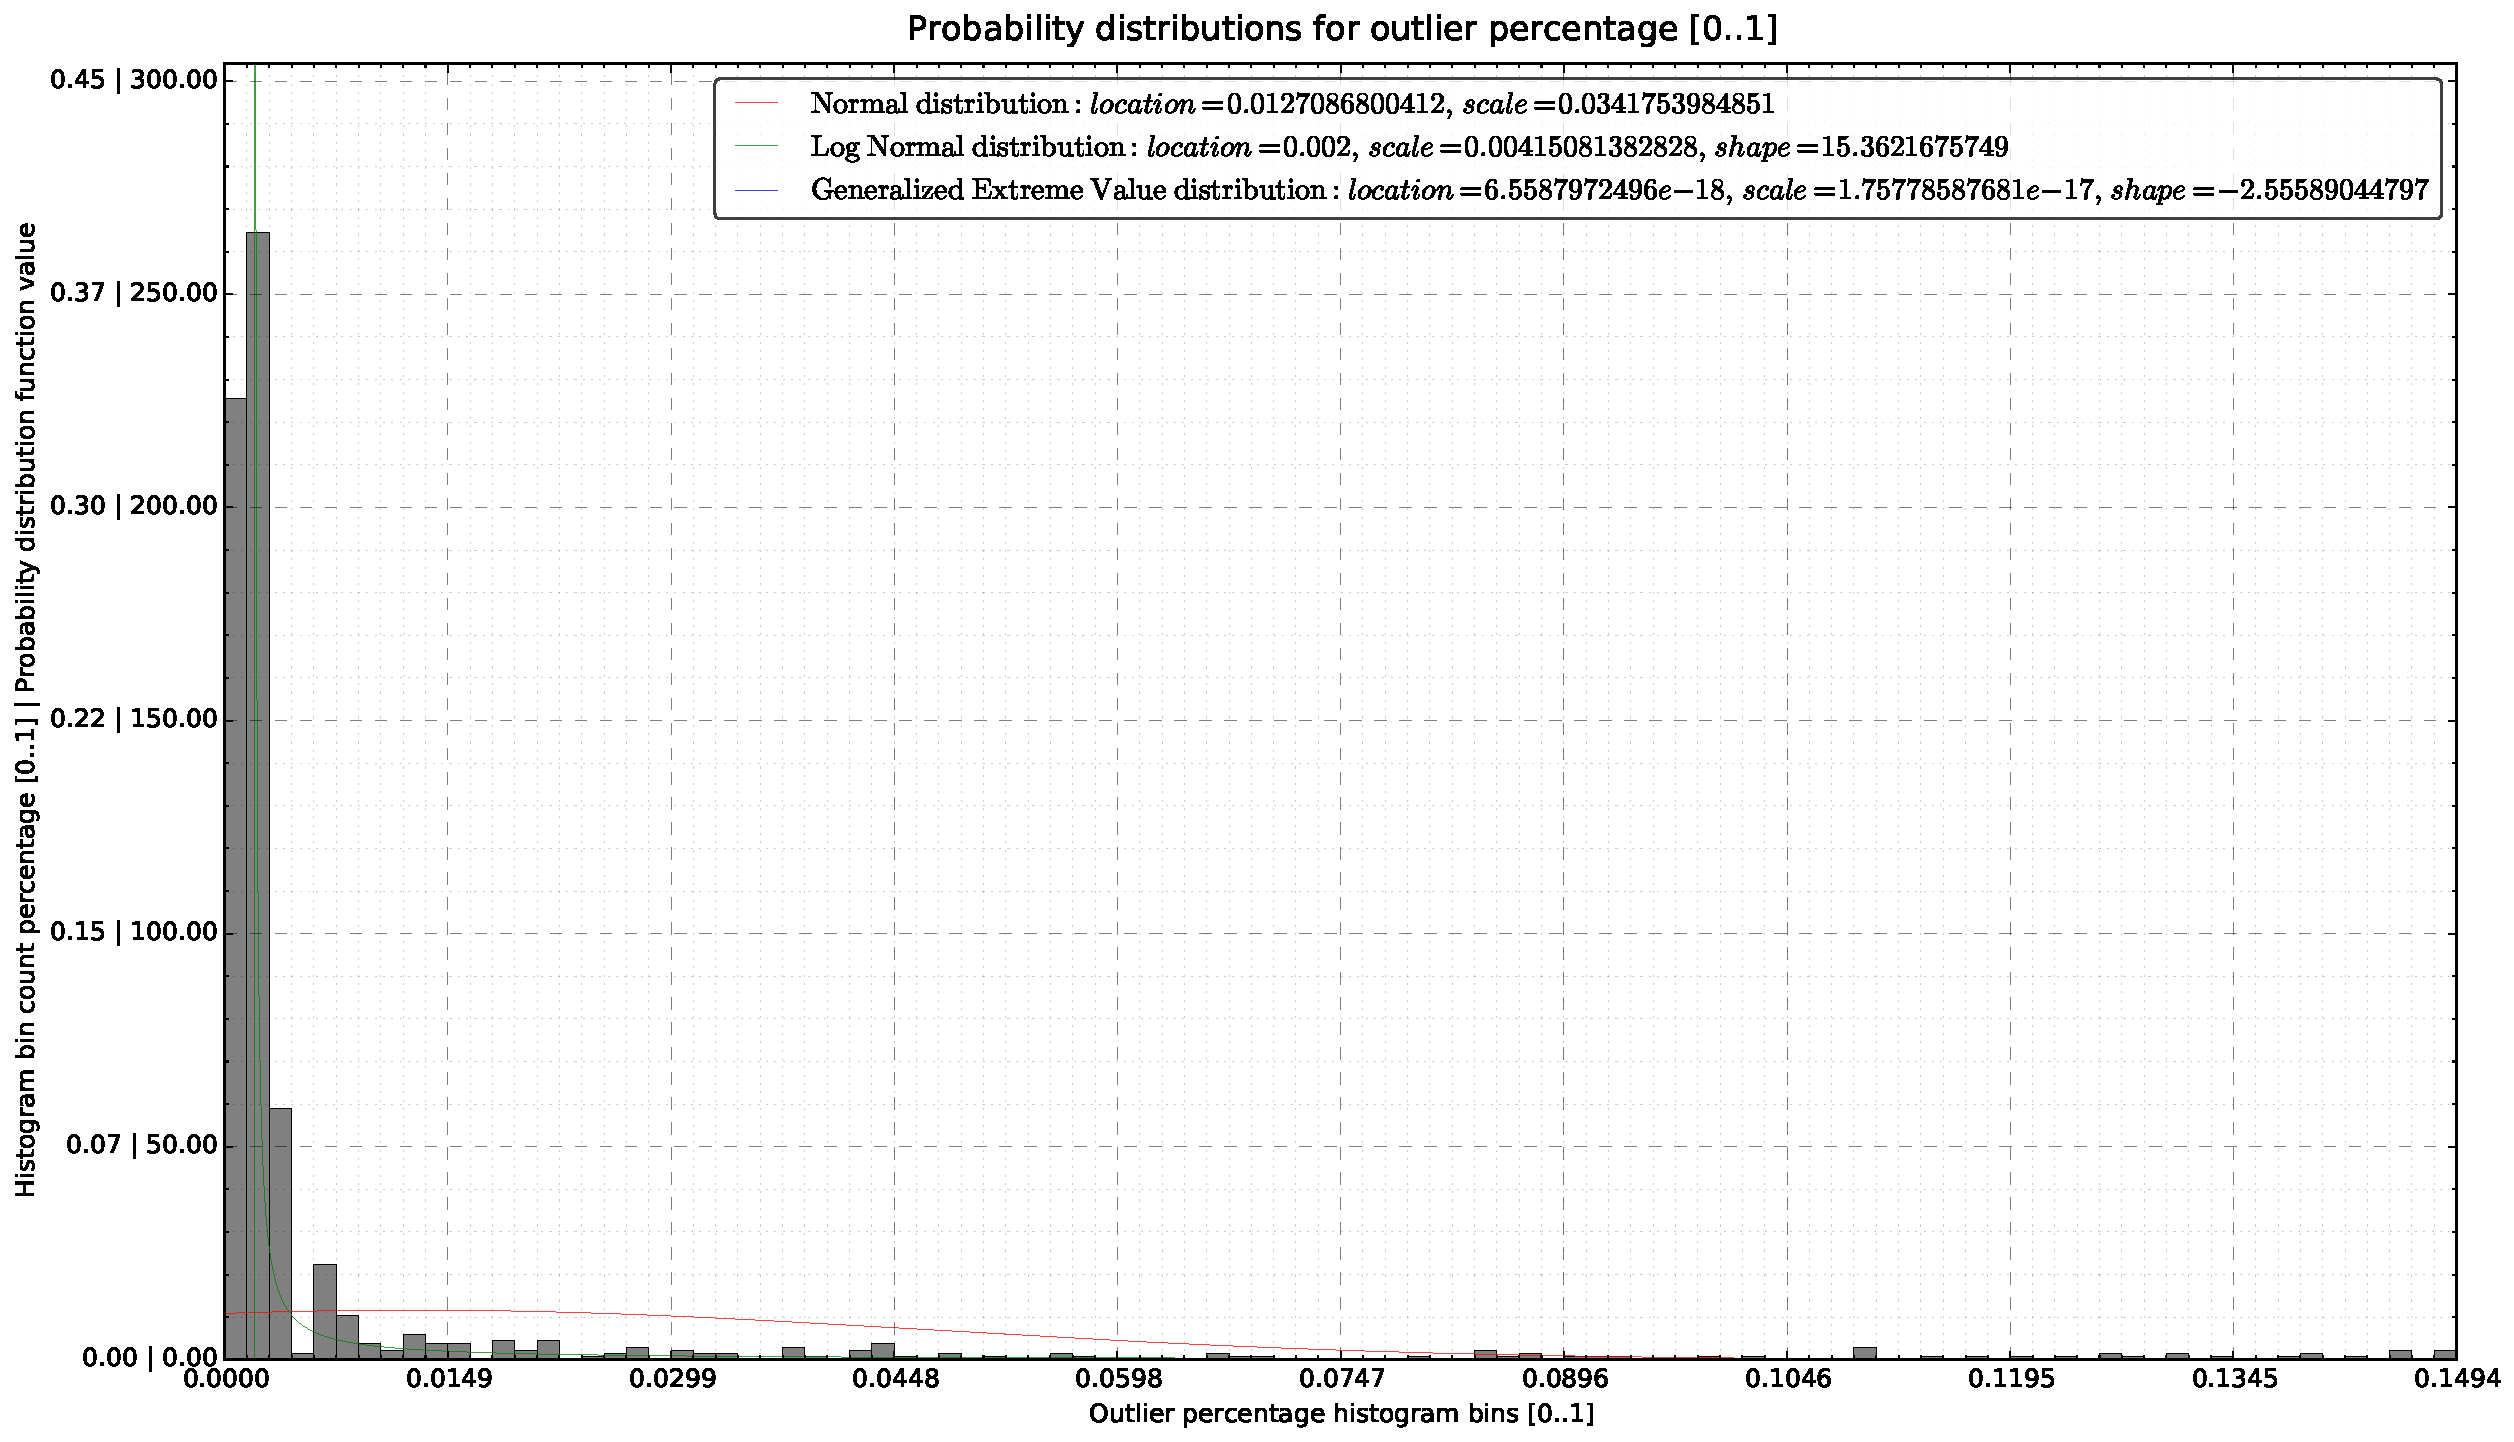
\includegraphics[width=0.69\textwidth]{appendices/tests-3dof/jarvis-robot/\currfilebase/graphs/outlier-percentage-distributions}
	\caption{Probability distributions for the ambient point cloud outlier percentage}
\end{figure}


\begin{figure}[H]
	\centering
	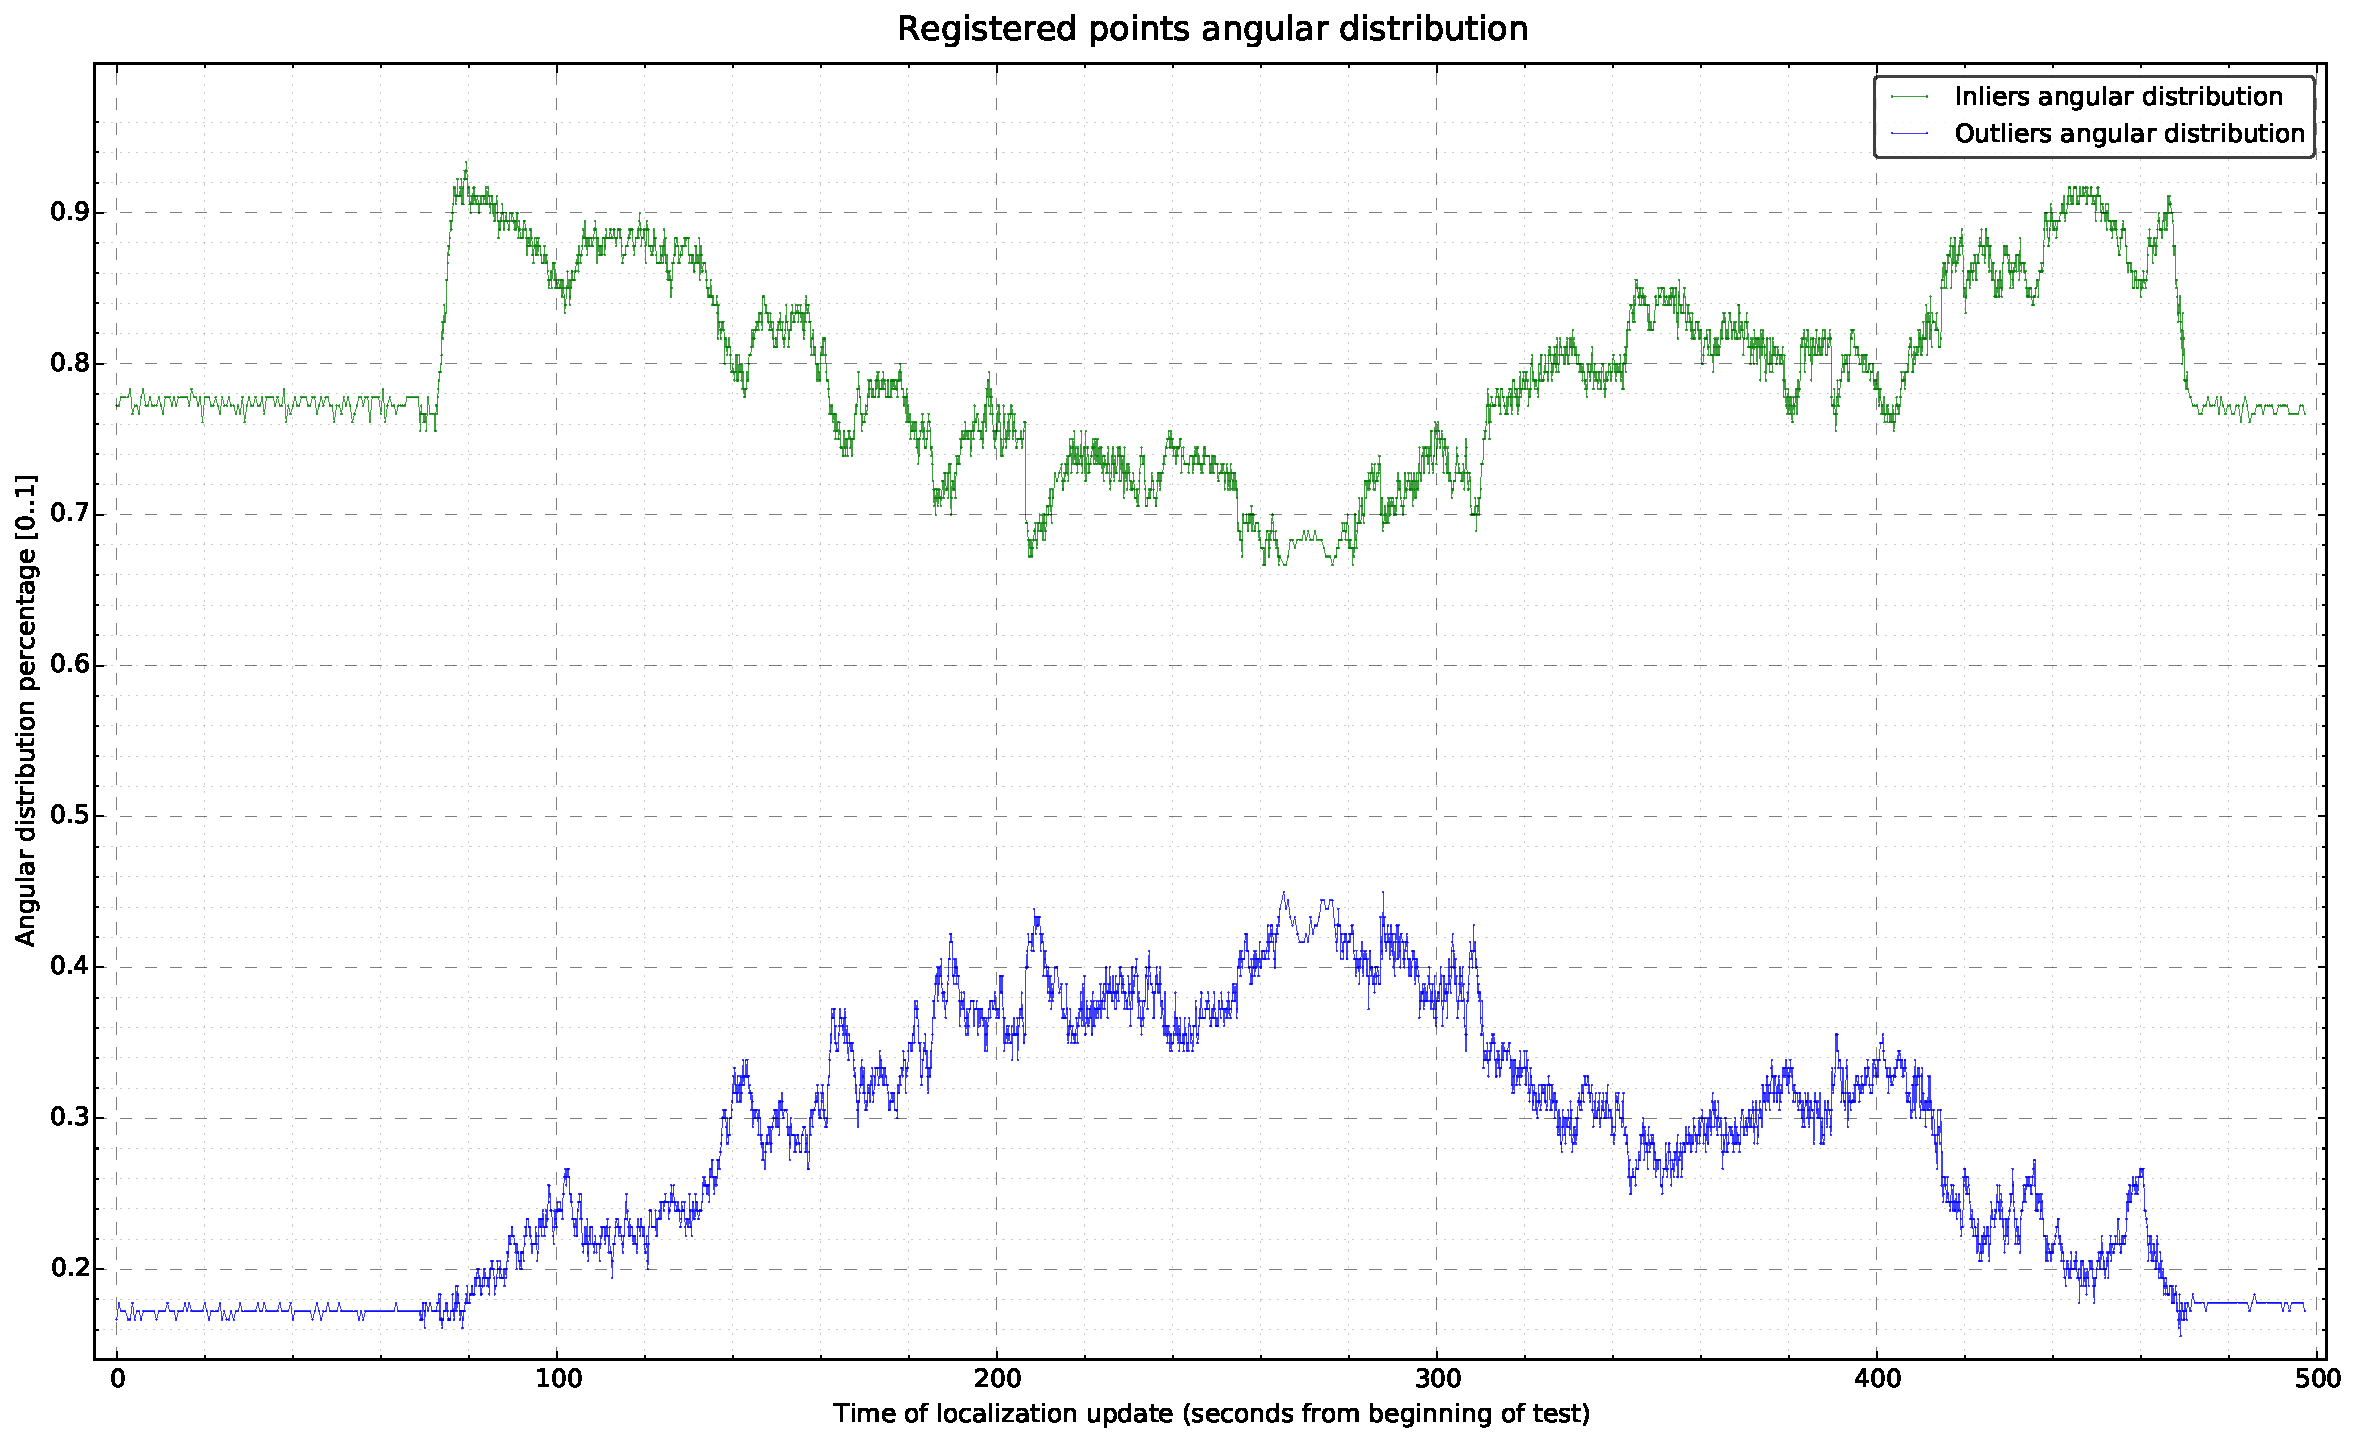
\includegraphics[width=0.69\textwidth]{appendices/tests-3dof/jarvis-robot/\currfilebase/graphs/registered-points-angular-distribution}
	\caption{Angular distribution percentage of registered points}
\end{figure}

\begin{figure}[H]
	\centering
	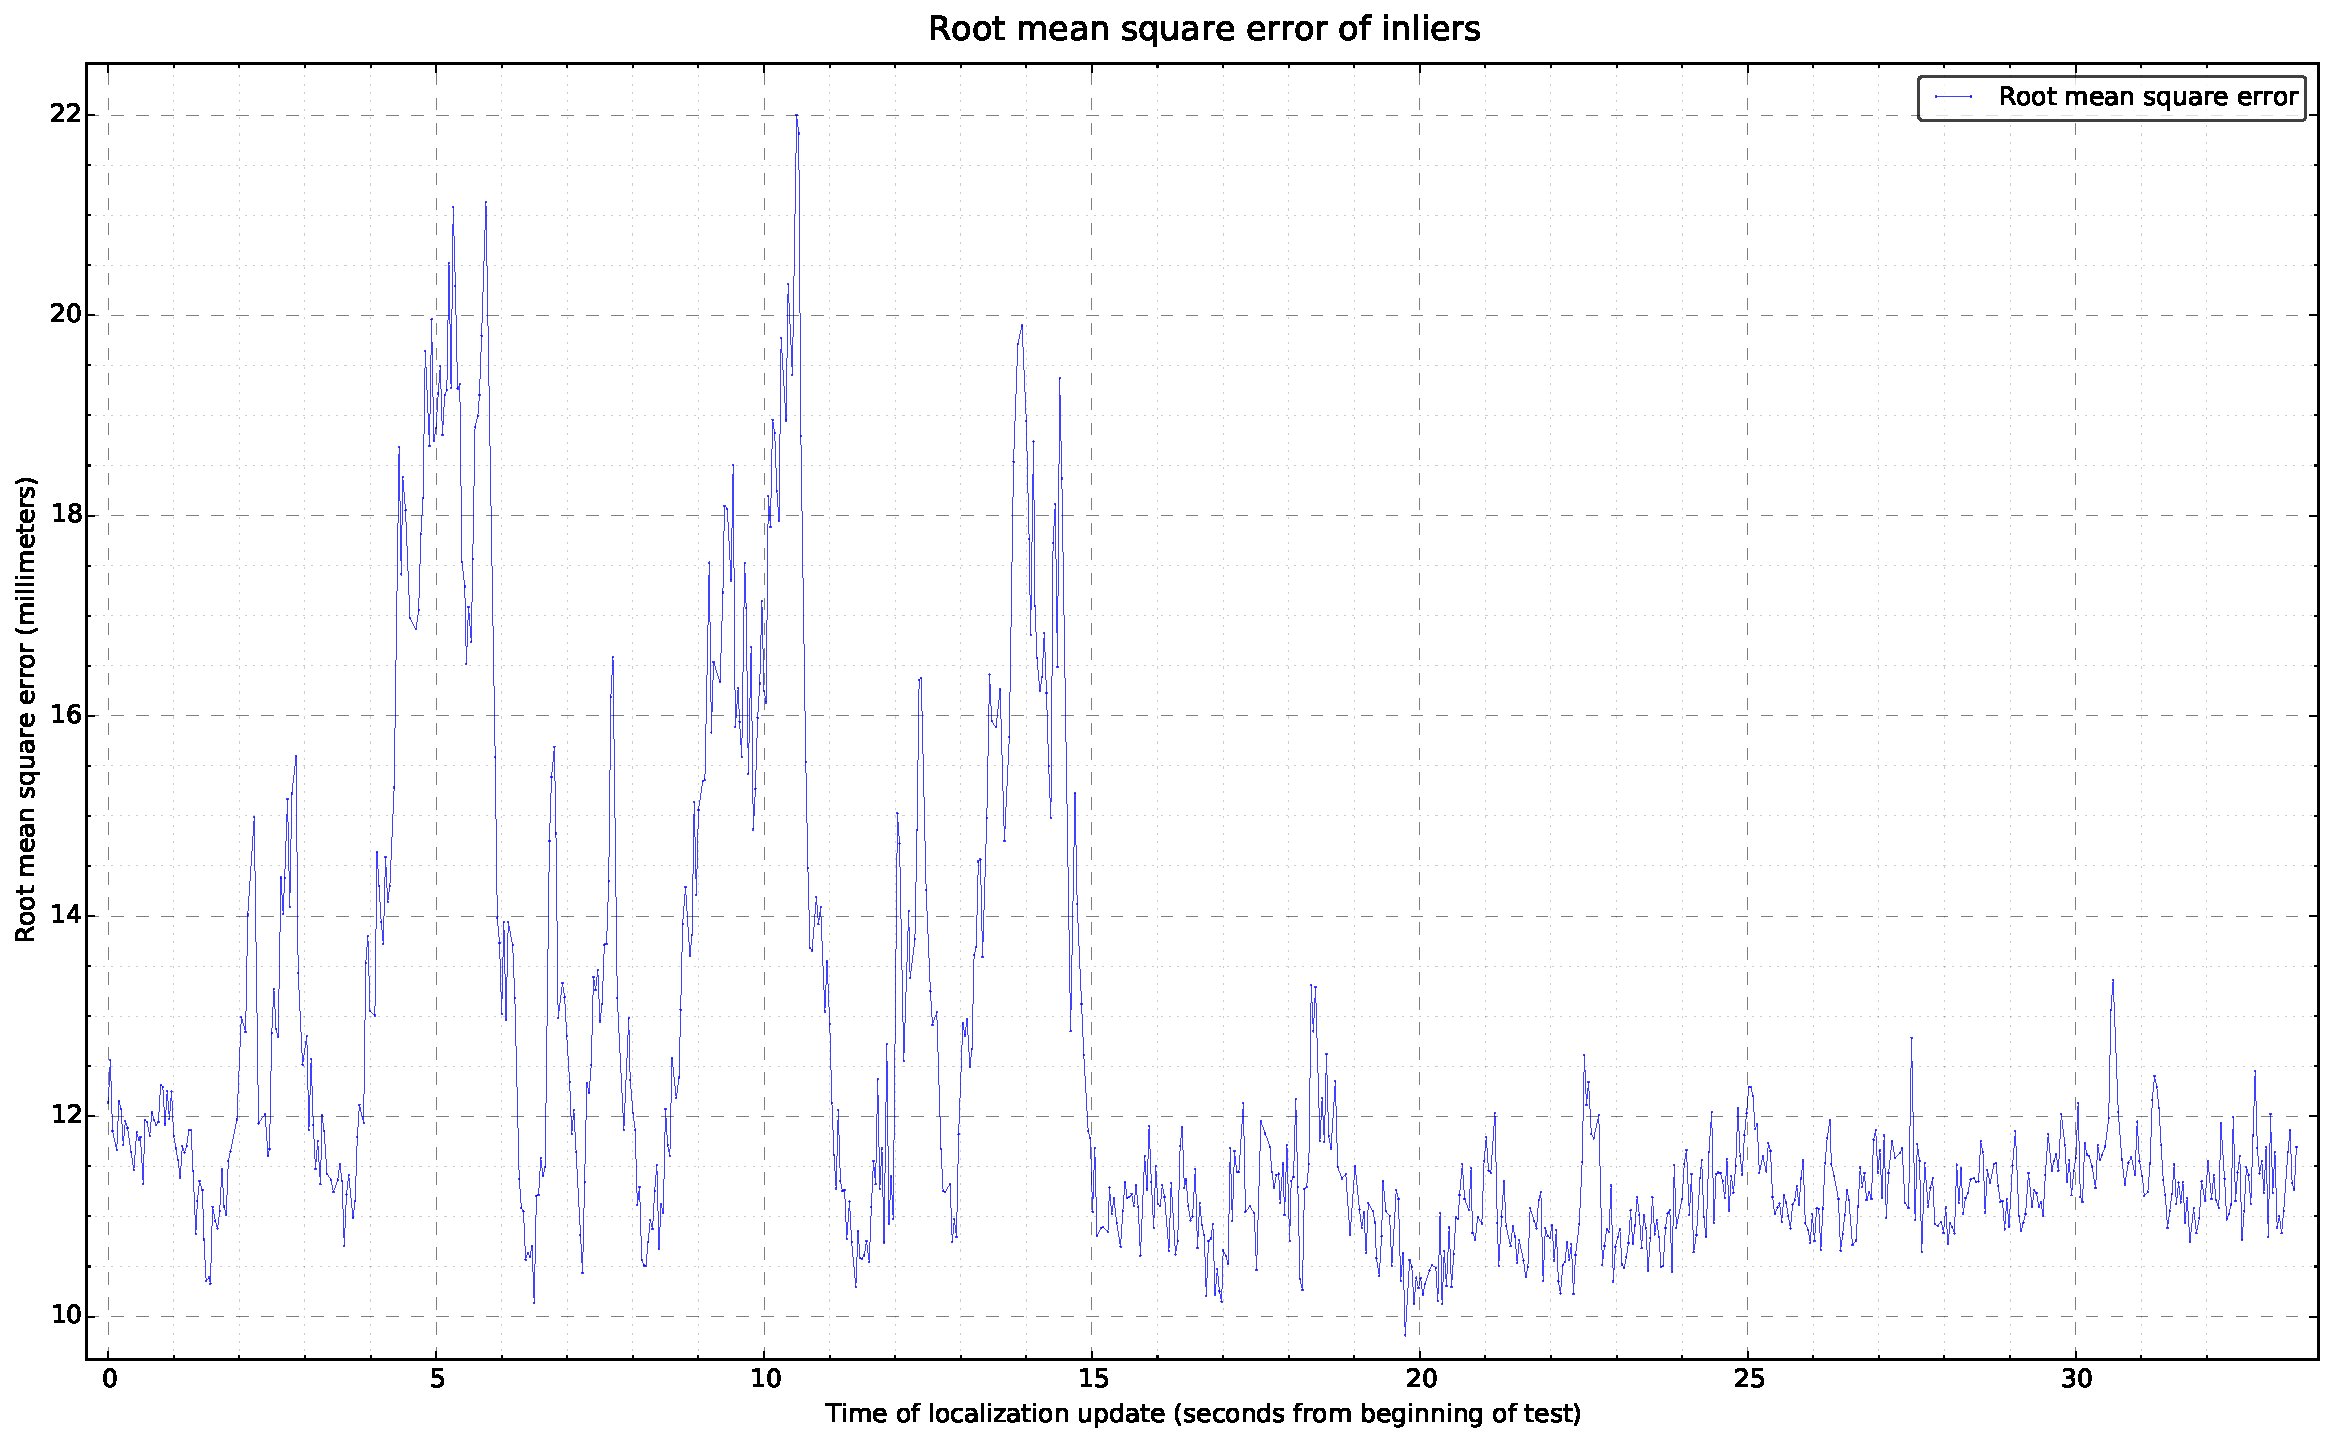
\includegraphics[width=0.69\textwidth]{appendices/tests-3dof/jarvis-robot/\currfilebase/graphs/root-mean-square-error-inliers}
	\caption{Root Mean Square Error of the inliers}
\end{figure}

\begin{figure}[H]
	\centering
	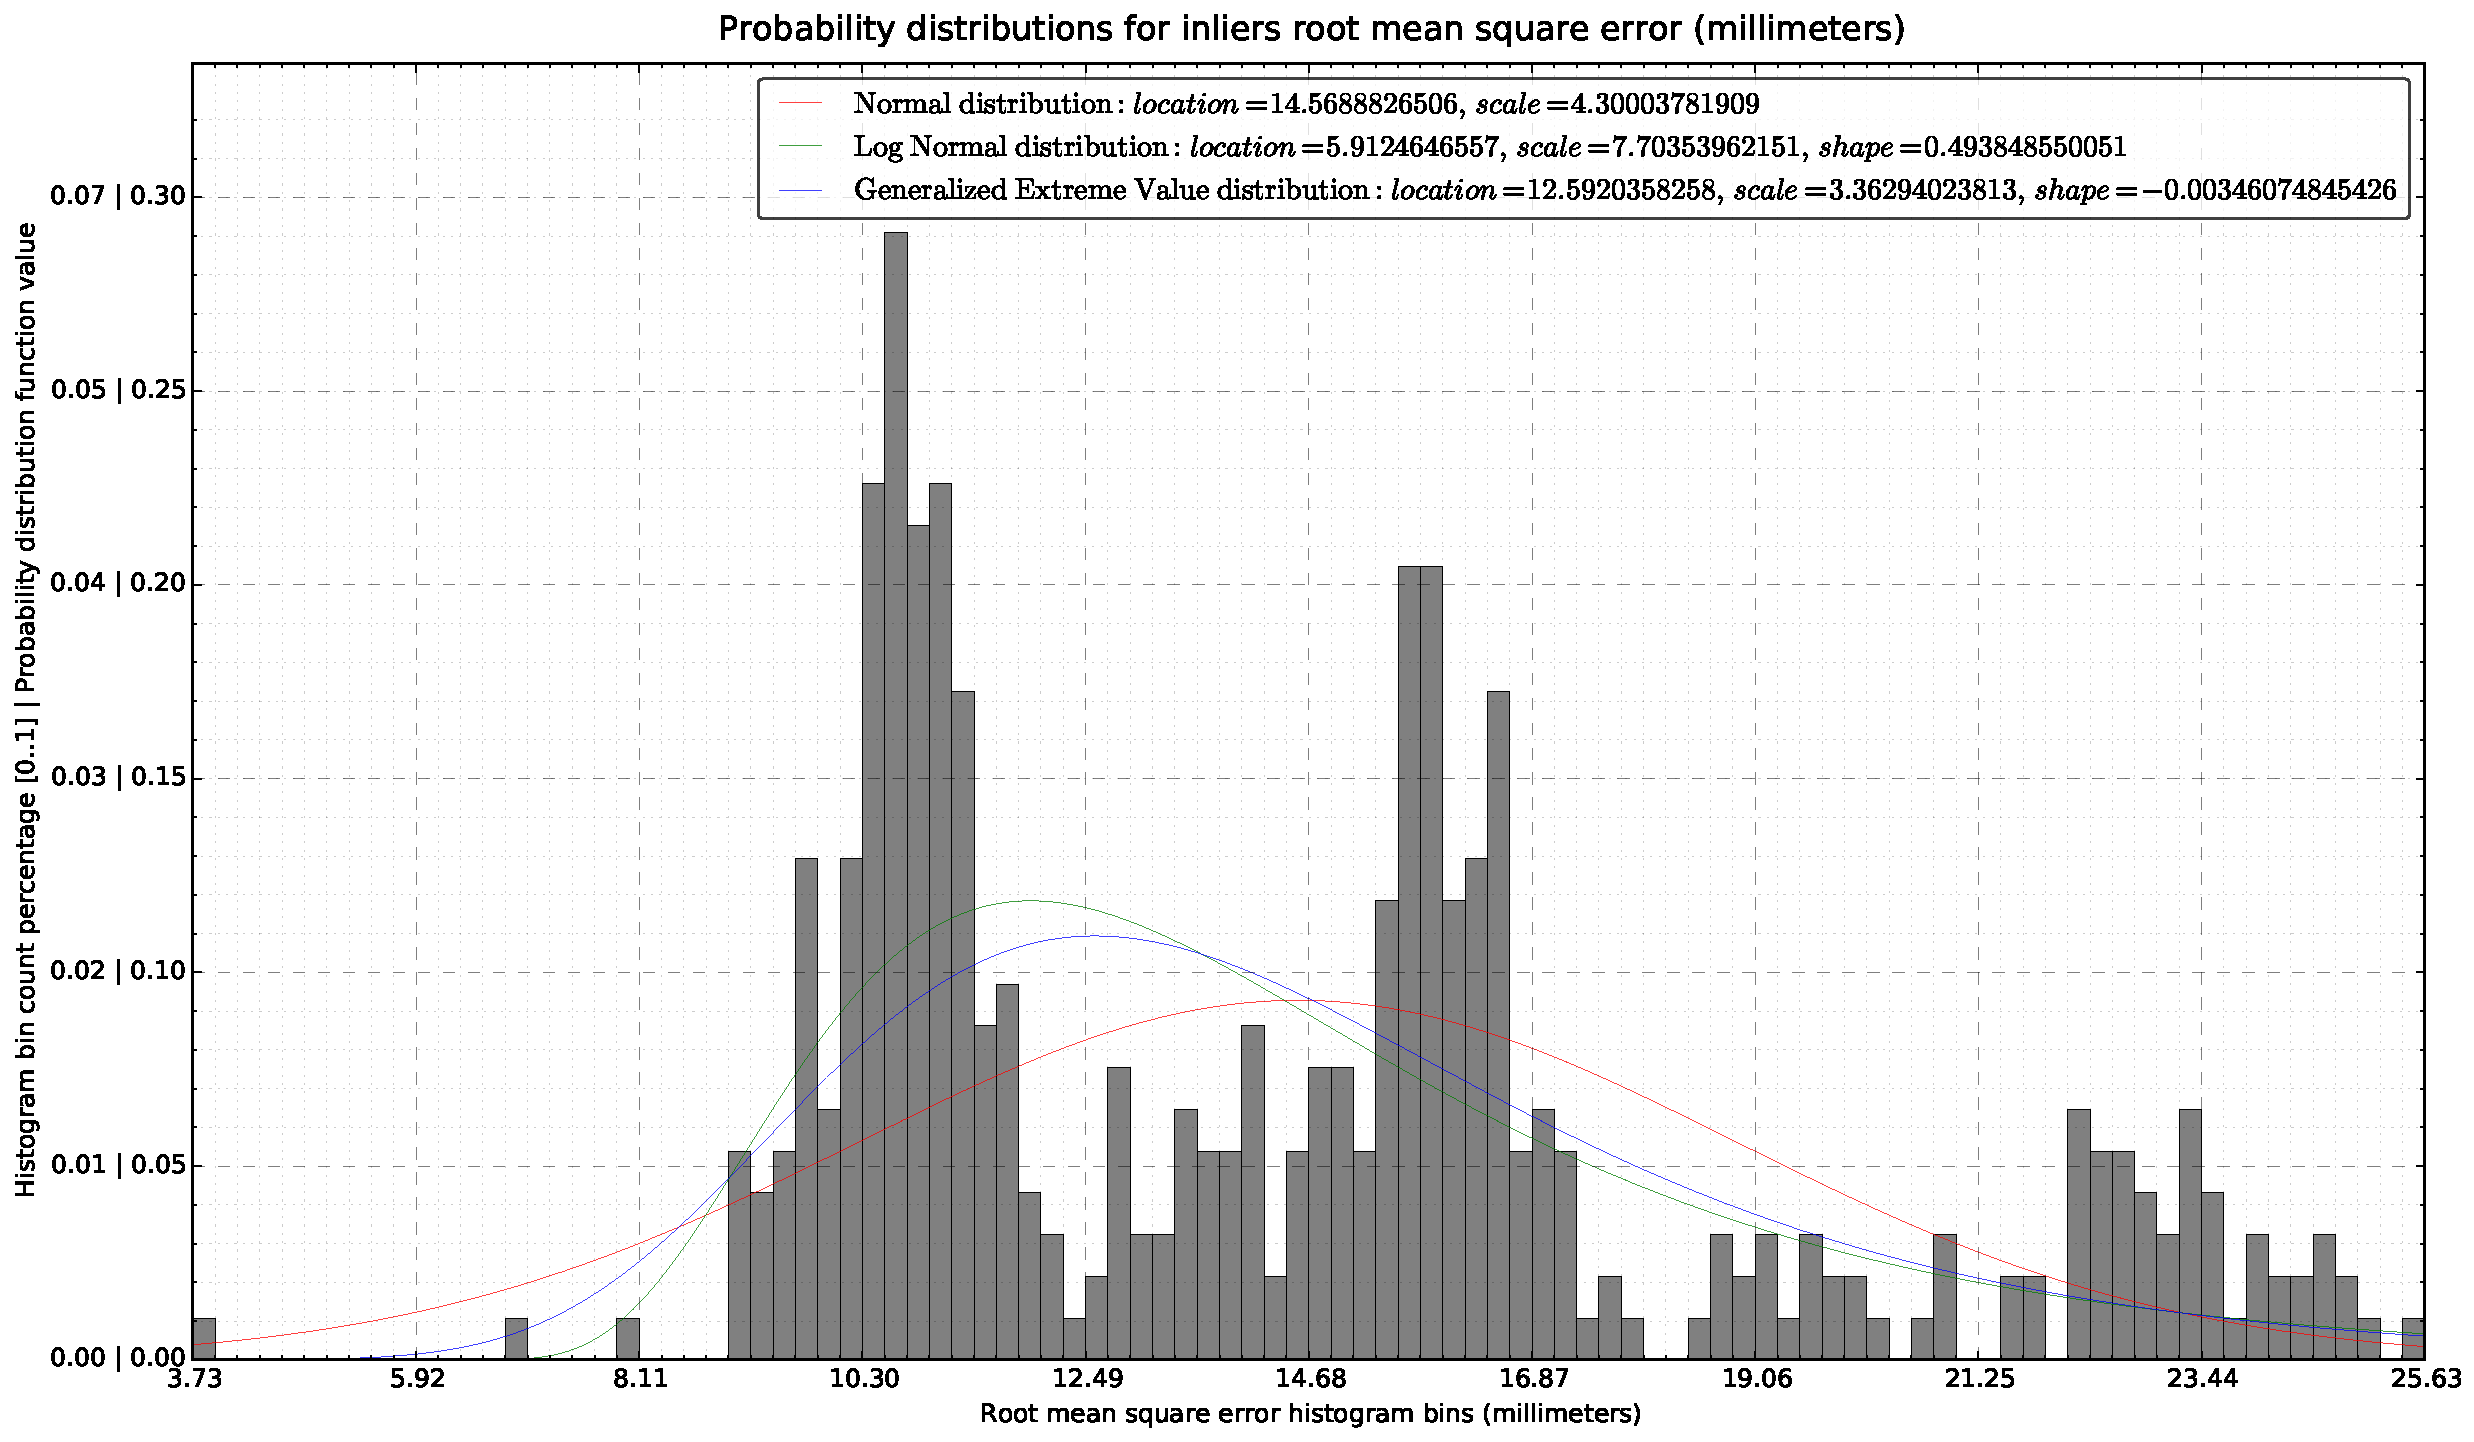
\includegraphics[width=0.69\textwidth]{appendices/tests-3dof/jarvis-robot/\currfilebase/graphs/root-mean-square-error-inliers-distributions}
	\caption{Probability distributions for the Root Mean Square Error of the inliers}
\end{figure}


%Computation times
\begin{figure}[H]
	\centering
	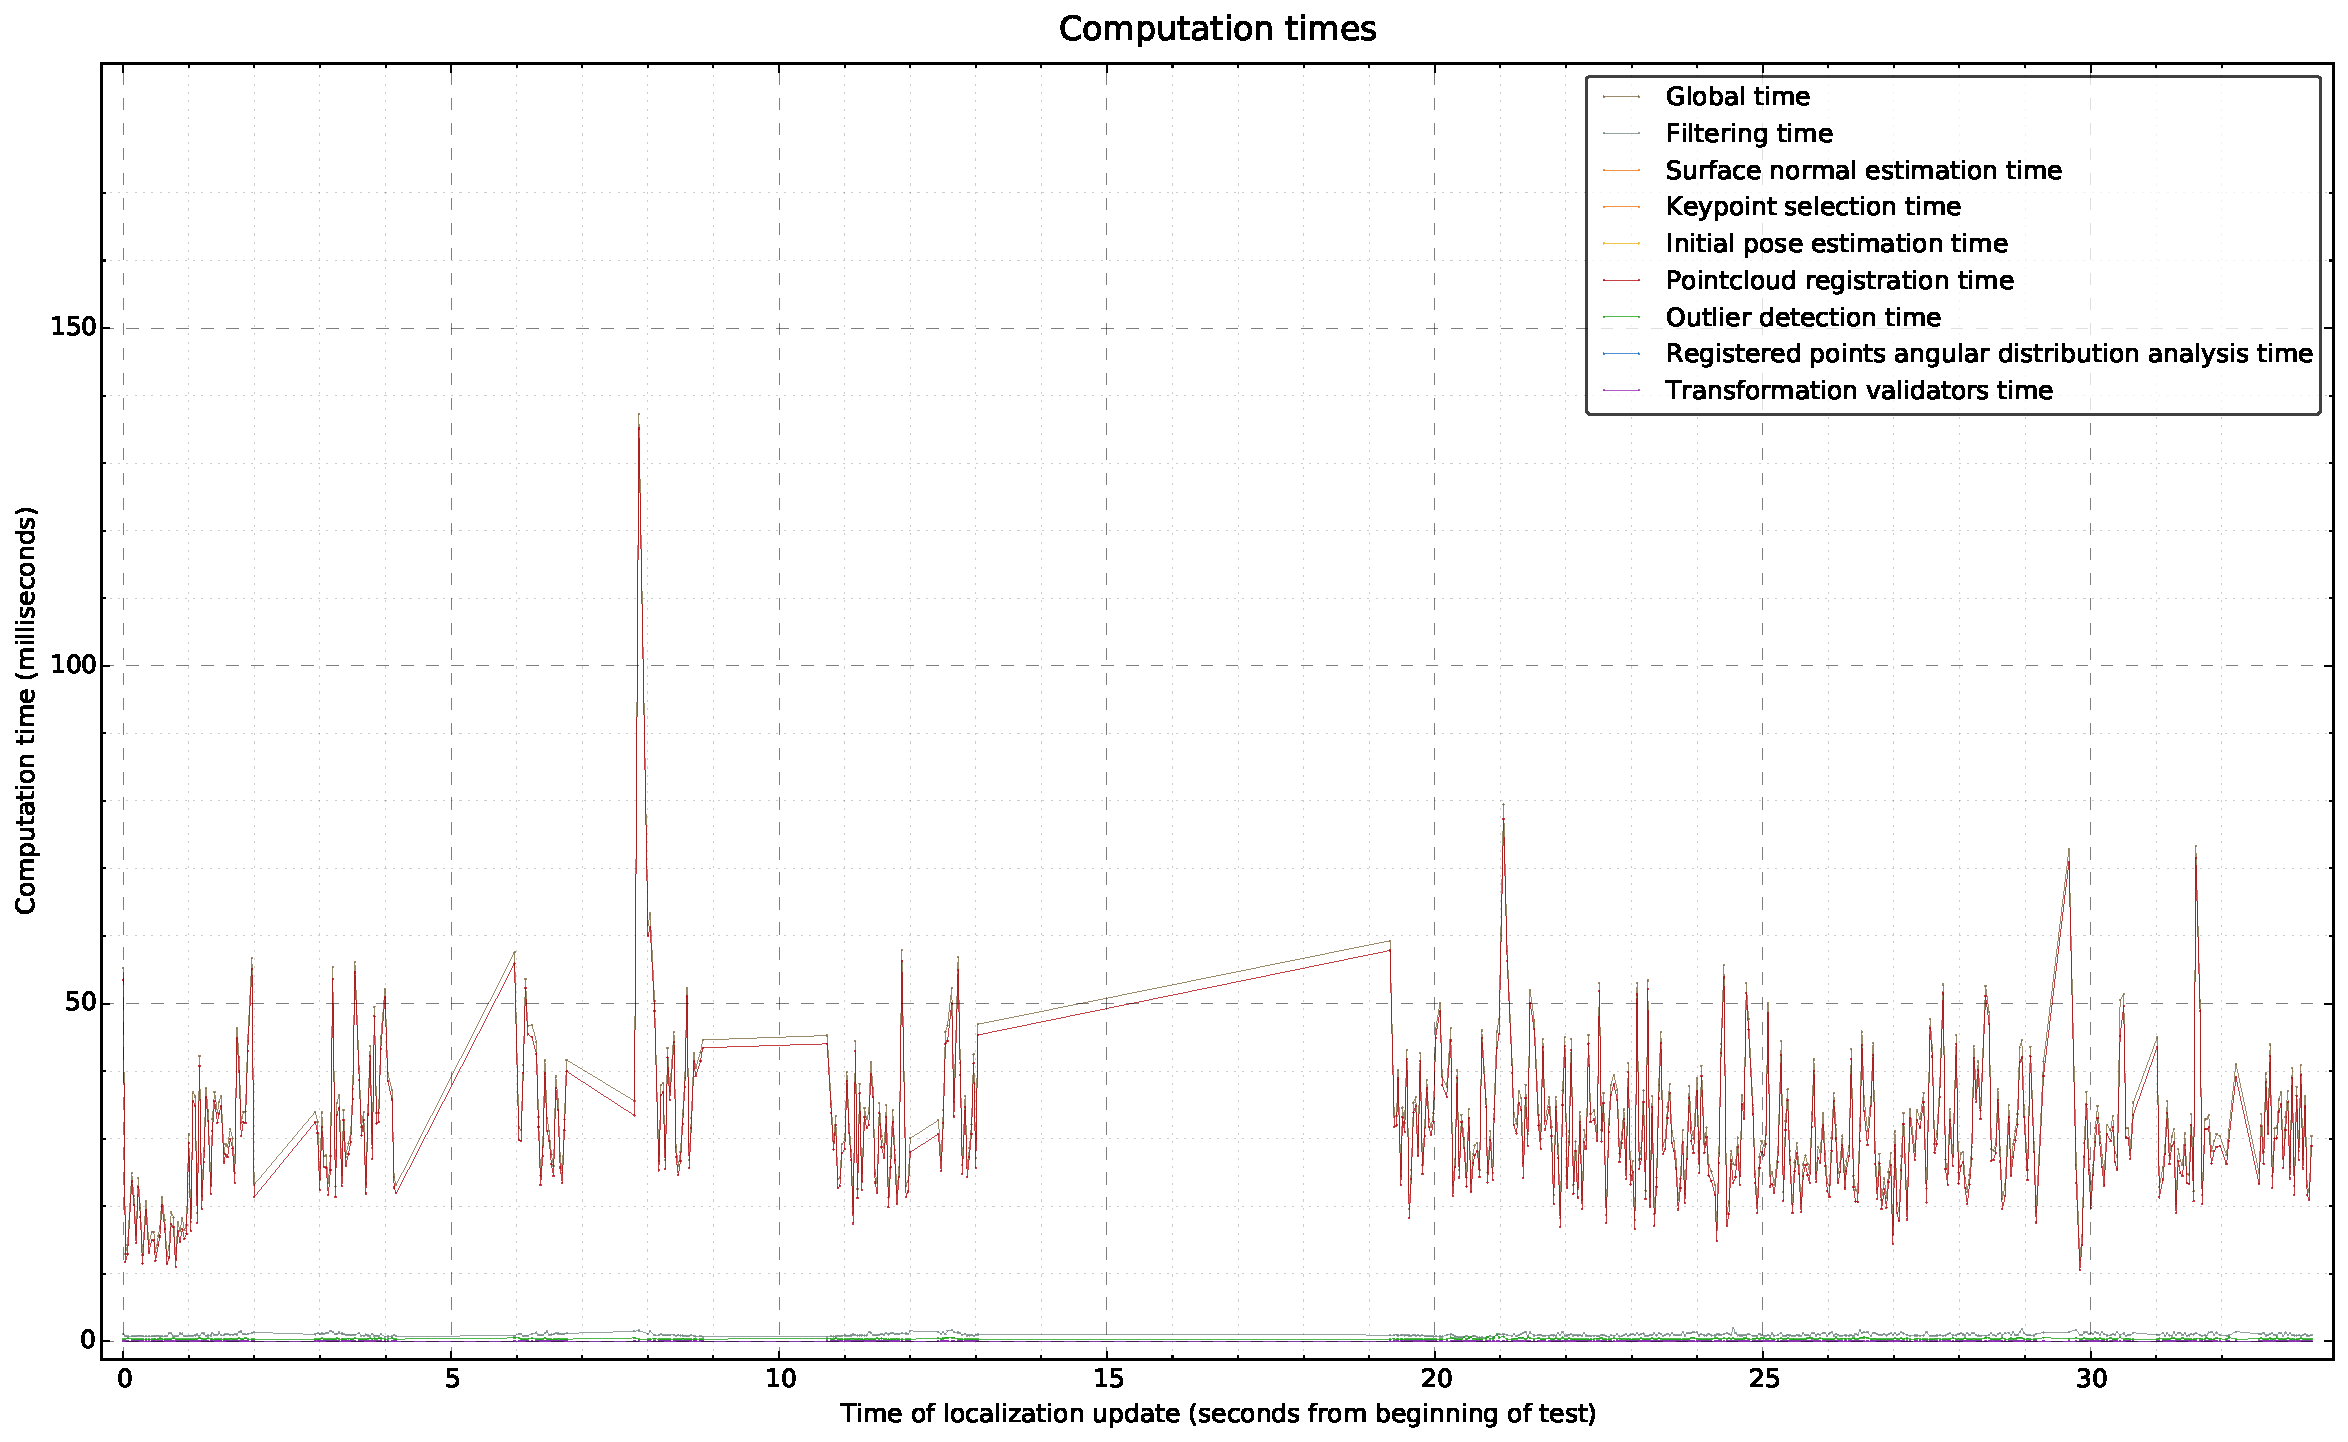
\includegraphics[width=0.69\textwidth]{appendices/tests-3dof/jarvis-robot/\currfilebase/graphs/computation-times-milliseconds}
	\caption{Localization system computation times}
\end{figure}

\begin{figure}[H]
	\centering
	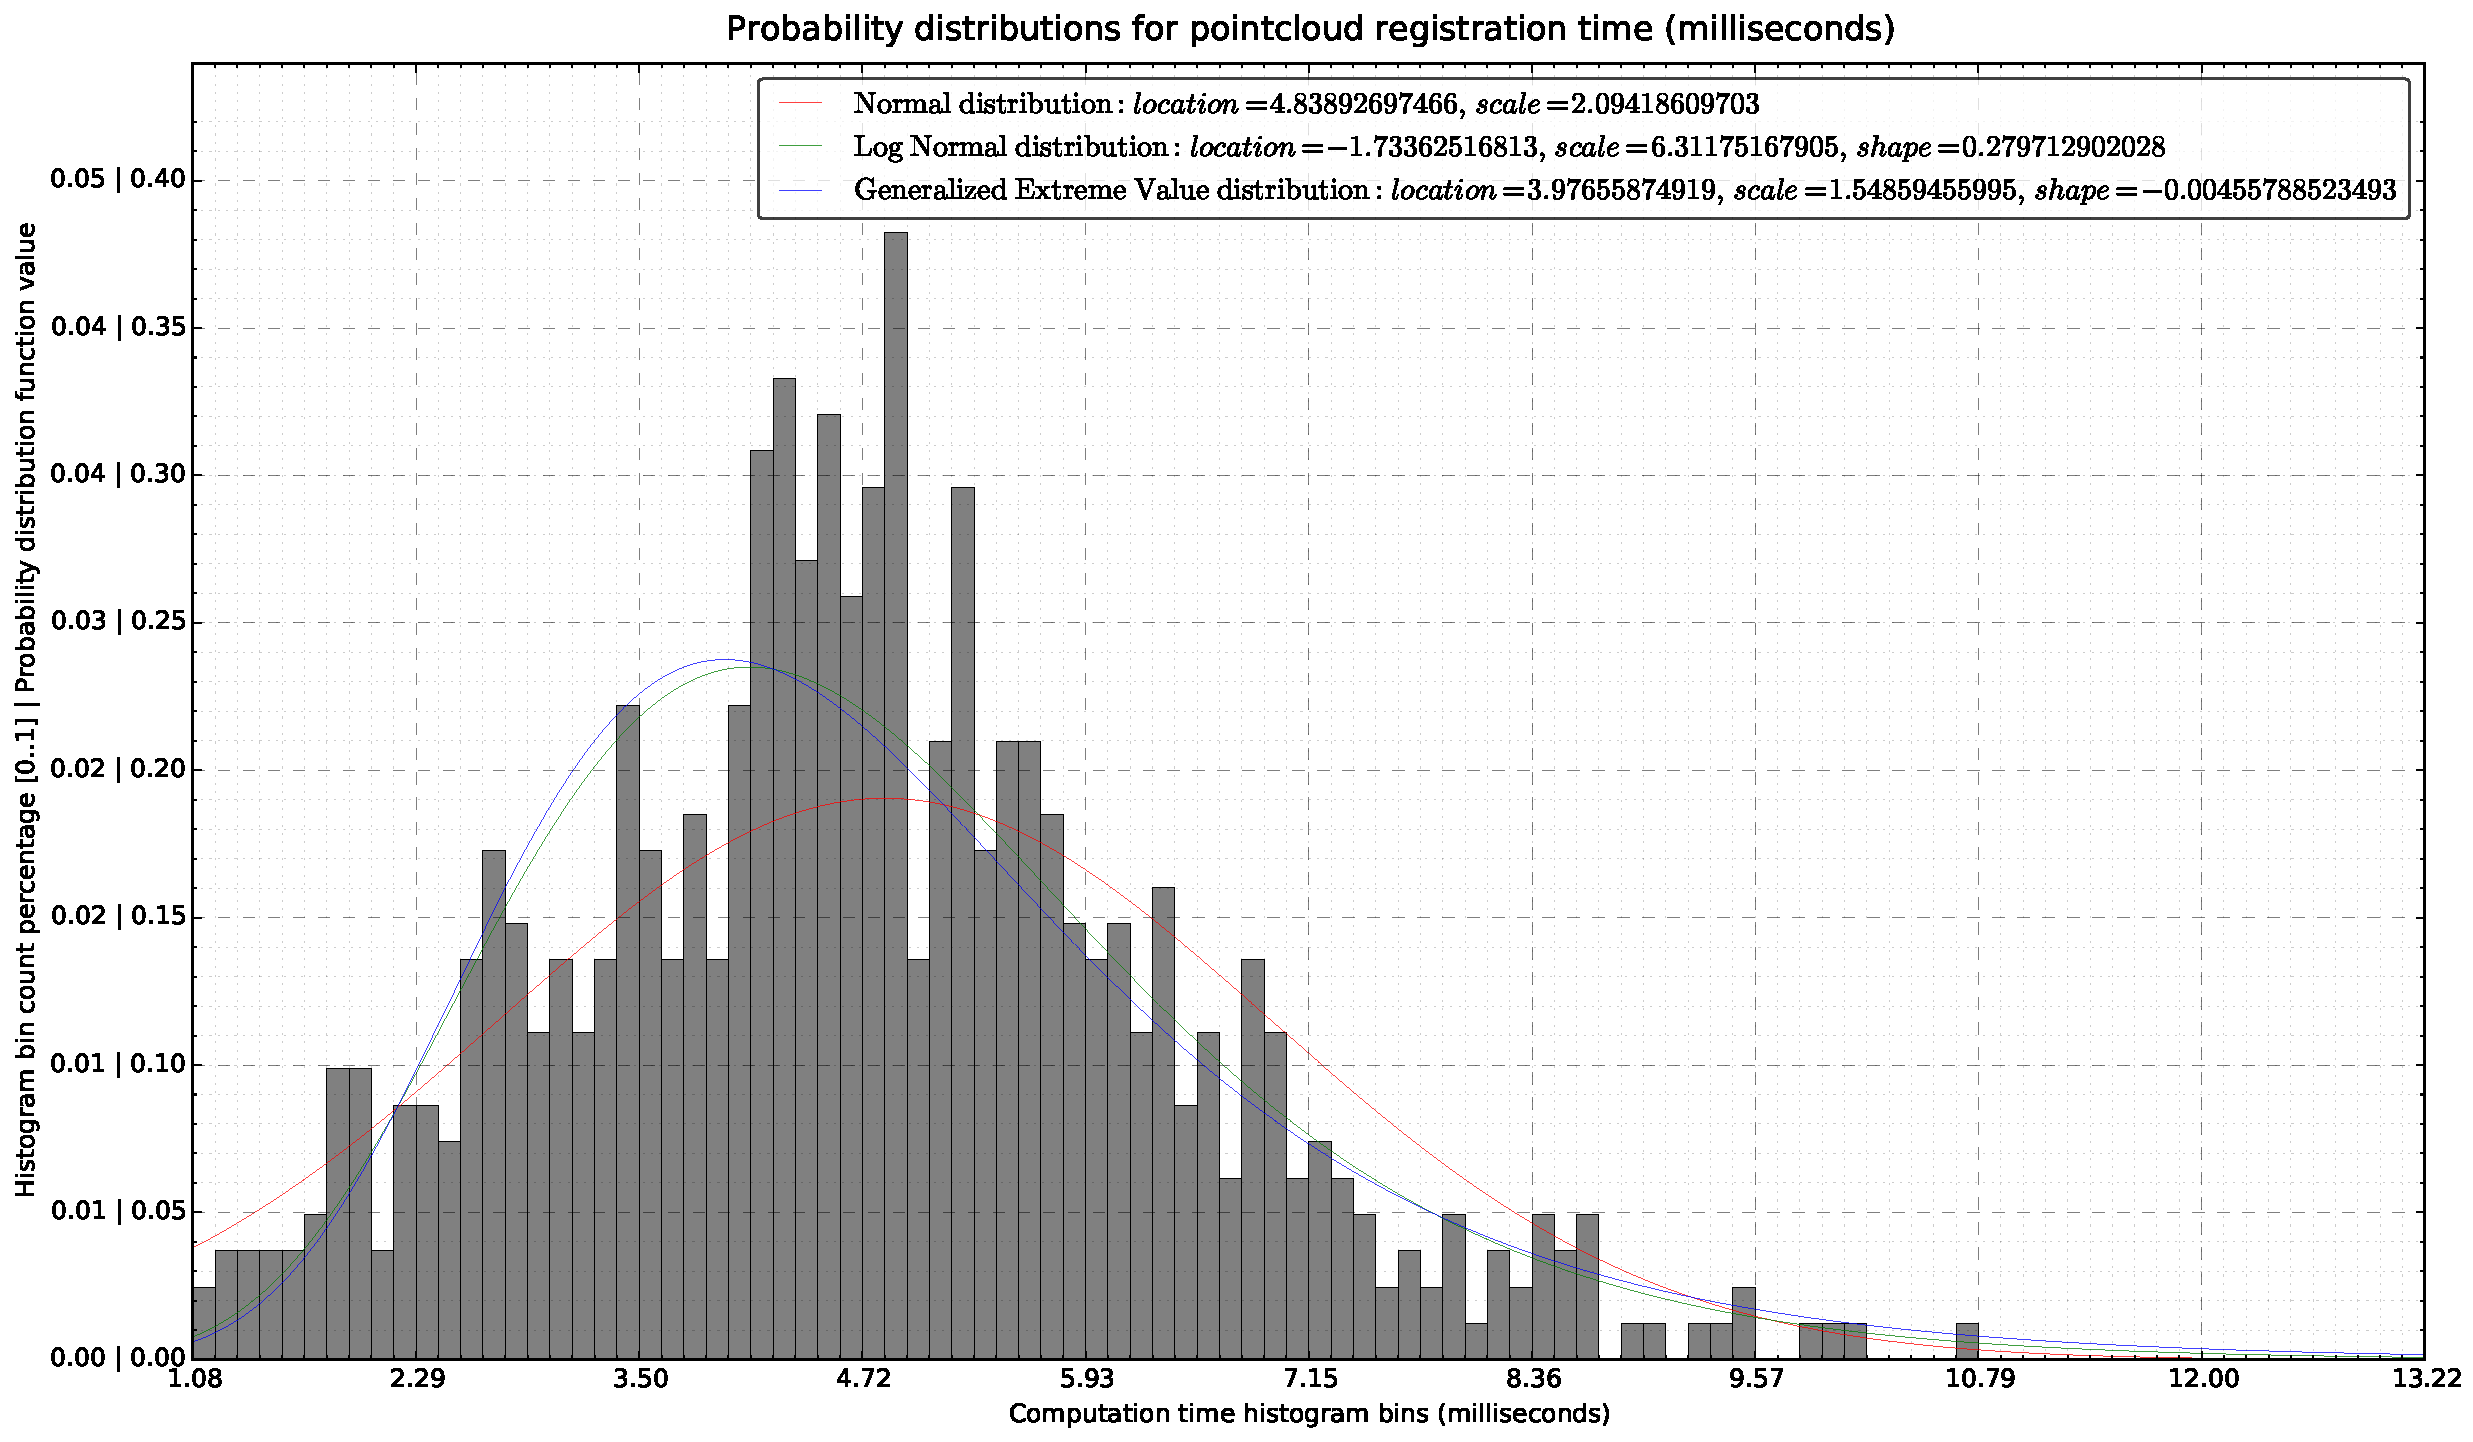
\includegraphics[width=0.69\textwidth]{appendices/tests-3dof/jarvis-robot/\currfilebase/graphs/computation-times-milliseconds-pointcloud-registration-time-distributions}
	\caption{Probability distributions for the point cloud registration time}
\end{figure}

\begin{figure}[H]
	\centering
	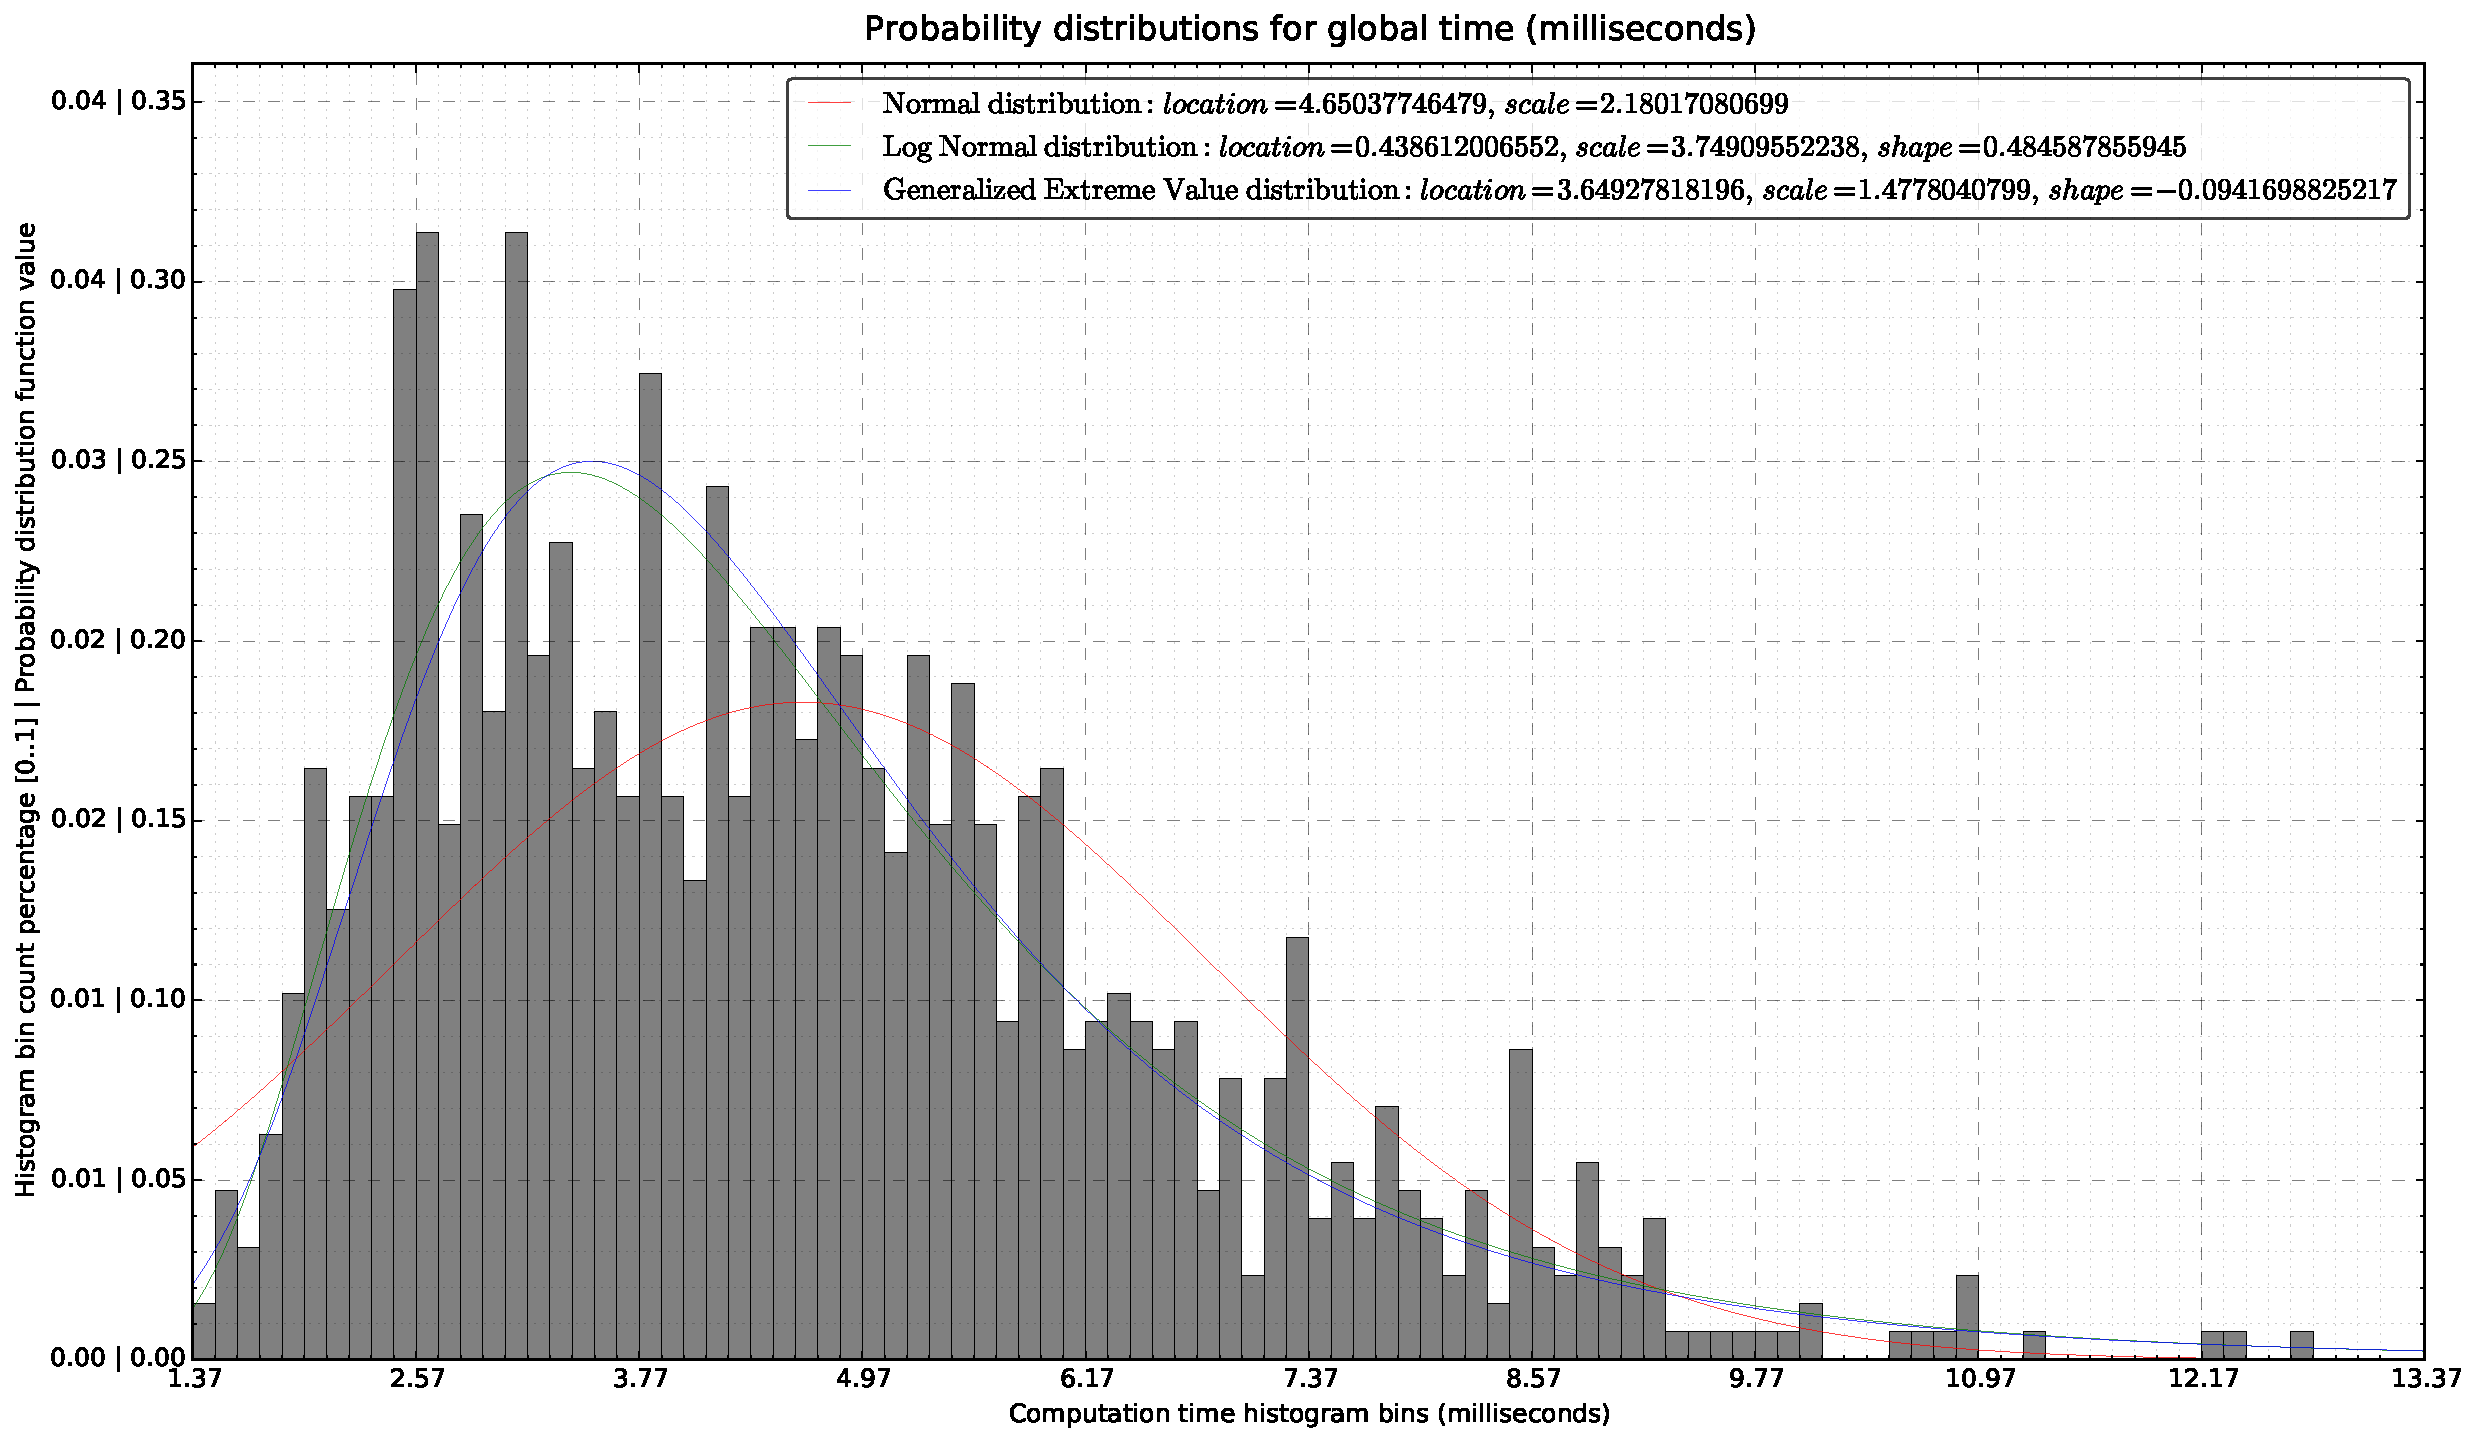
\includegraphics[width=0.69\textwidth]{appendices/tests-3dof/jarvis-robot/\currfilebase/graphs/computation-times-milliseconds-global-time-distributions}
	\caption{Probability distributions for the localization system global computation time}
\end{figure}

\subsection{Rounded path using the Jarvis robot at 30 cm/s}\label{subsec:appendix-a_jarvis-robot-tests_rounded-path-using-the-jarvis-robot-at-30-cm-s}

The figures in this section show the detailed results of the test performed with the Jarvis robot with a 10 mm resolution map in the RoboCup field following a rounded path and moving at 30 cm/s.


%Animated paths
\begin{figure}[H]
	\centering
	\animategraphics[width=0.8\textwidth,loop,autoplay,controls]{1}{appendices/tests-3dof/jarvis-robot/\currfilebase/images-ground-truth/image}{1}{10}
	\caption{Animation of laser scans using the ground truth poses}
\end{figure}

\begin{figure}[H]
	\centering
	\animategraphics[width=0.8\textwidth,loop,autoplay,controls]{1}{appendices/tests-3dof/jarvis-robot/\currfilebase/images-drl/image}{1}{10}
	\caption{Animation of laser scans using the localization system poses}
\end{figure}

\begin{figure}[H]
	\centering
	\animategraphics[width=0.8\textwidth,loop,autoplay,controls]{1}{appendices/tests-3dof/jarvis-robot/\currfilebase/images-amcl/image}{1}{10}
	\caption{Animation of laser scans using the \glsentrytext{amcl} poses}
\end{figure}


%Laser assembly
\begin{figure}[H]
	\centering
	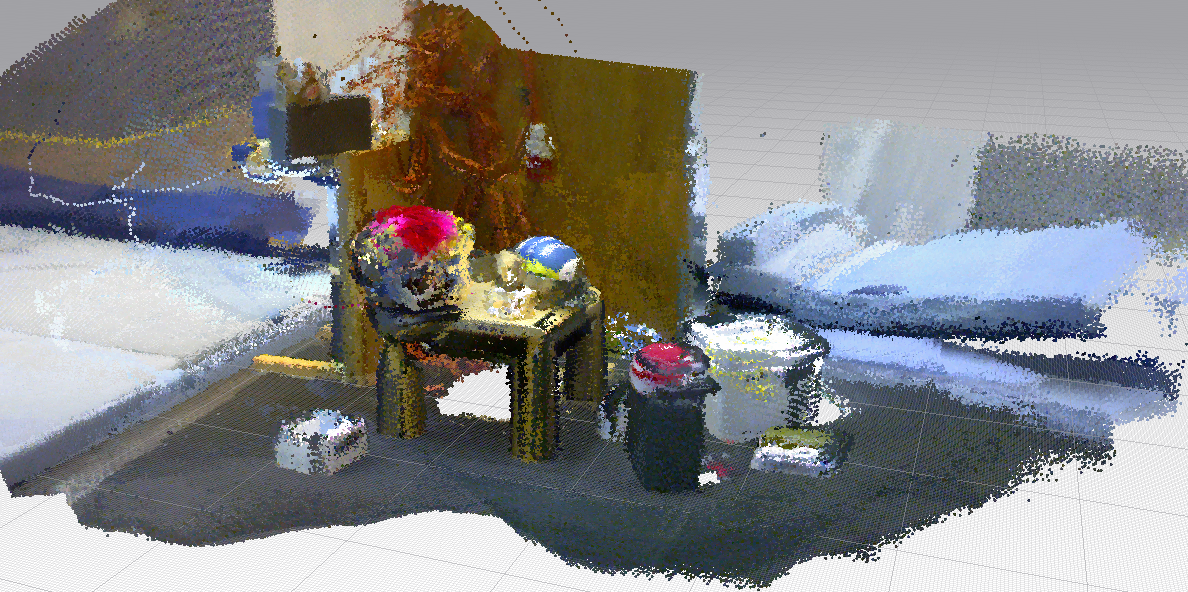
\includegraphics[width=0.993\textwidth]{appendices/tests-3dof/jarvis-robot/\currfilebase/ground-truth-cumulative}
	\caption{Laser scans assembled on top of the map using the ground truth poses}
\end{figure}

\begin{figure}[H]
	\centering
	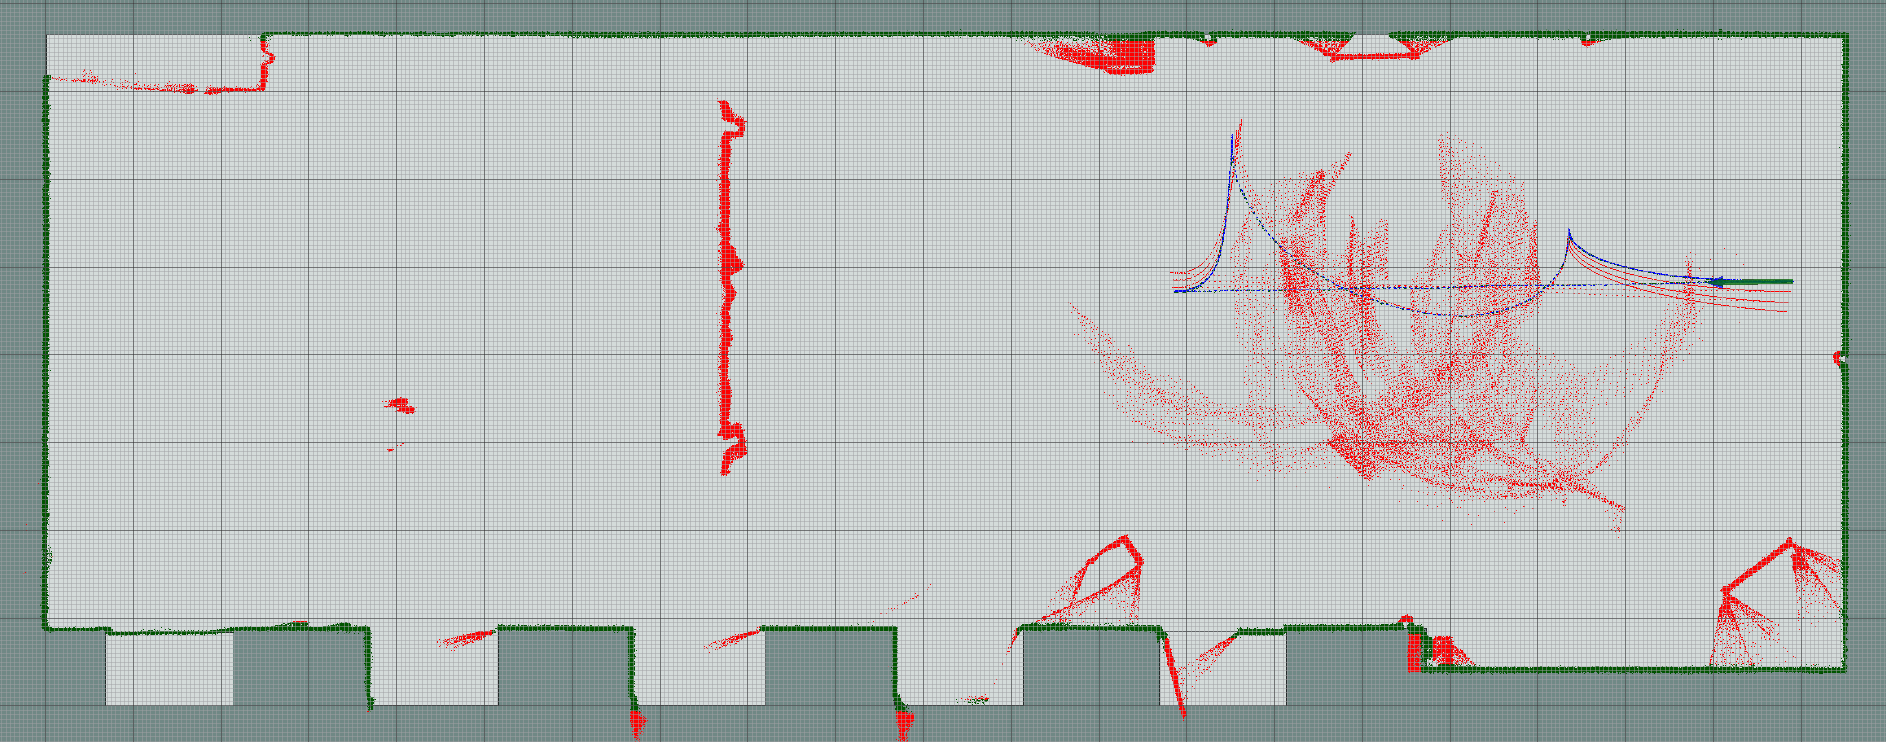
\includegraphics[width=0.993\textwidth]{appendices/tests-3dof/jarvis-robot/\currfilebase/drl-cumulative}
	\caption{Laser scans assembled on top of the map using the localization system poses}
\end{figure}

\begin{figure}[H]
	\centering
	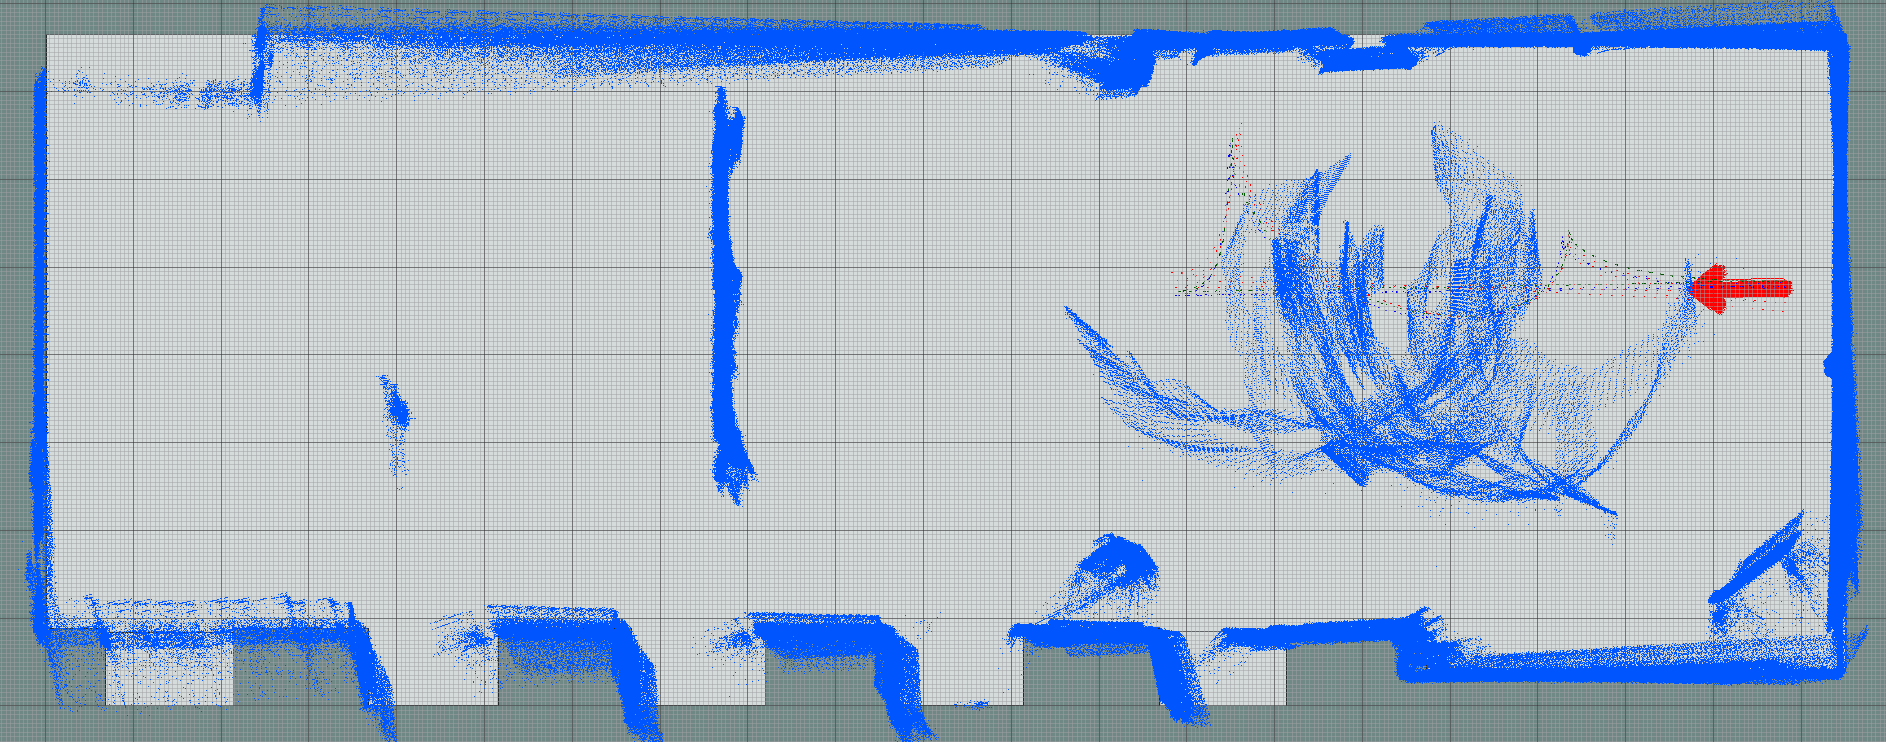
\includegraphics[width=0.993\textwidth]{appendices/tests-3dof/jarvis-robot/\currfilebase/amcl-cumulative}
	\caption{Laser scans assembled on top of the map using the \glsentrytext{amcl} poses}
\end{figure}


%Paths
\begin{figure}[H]
	\centering
	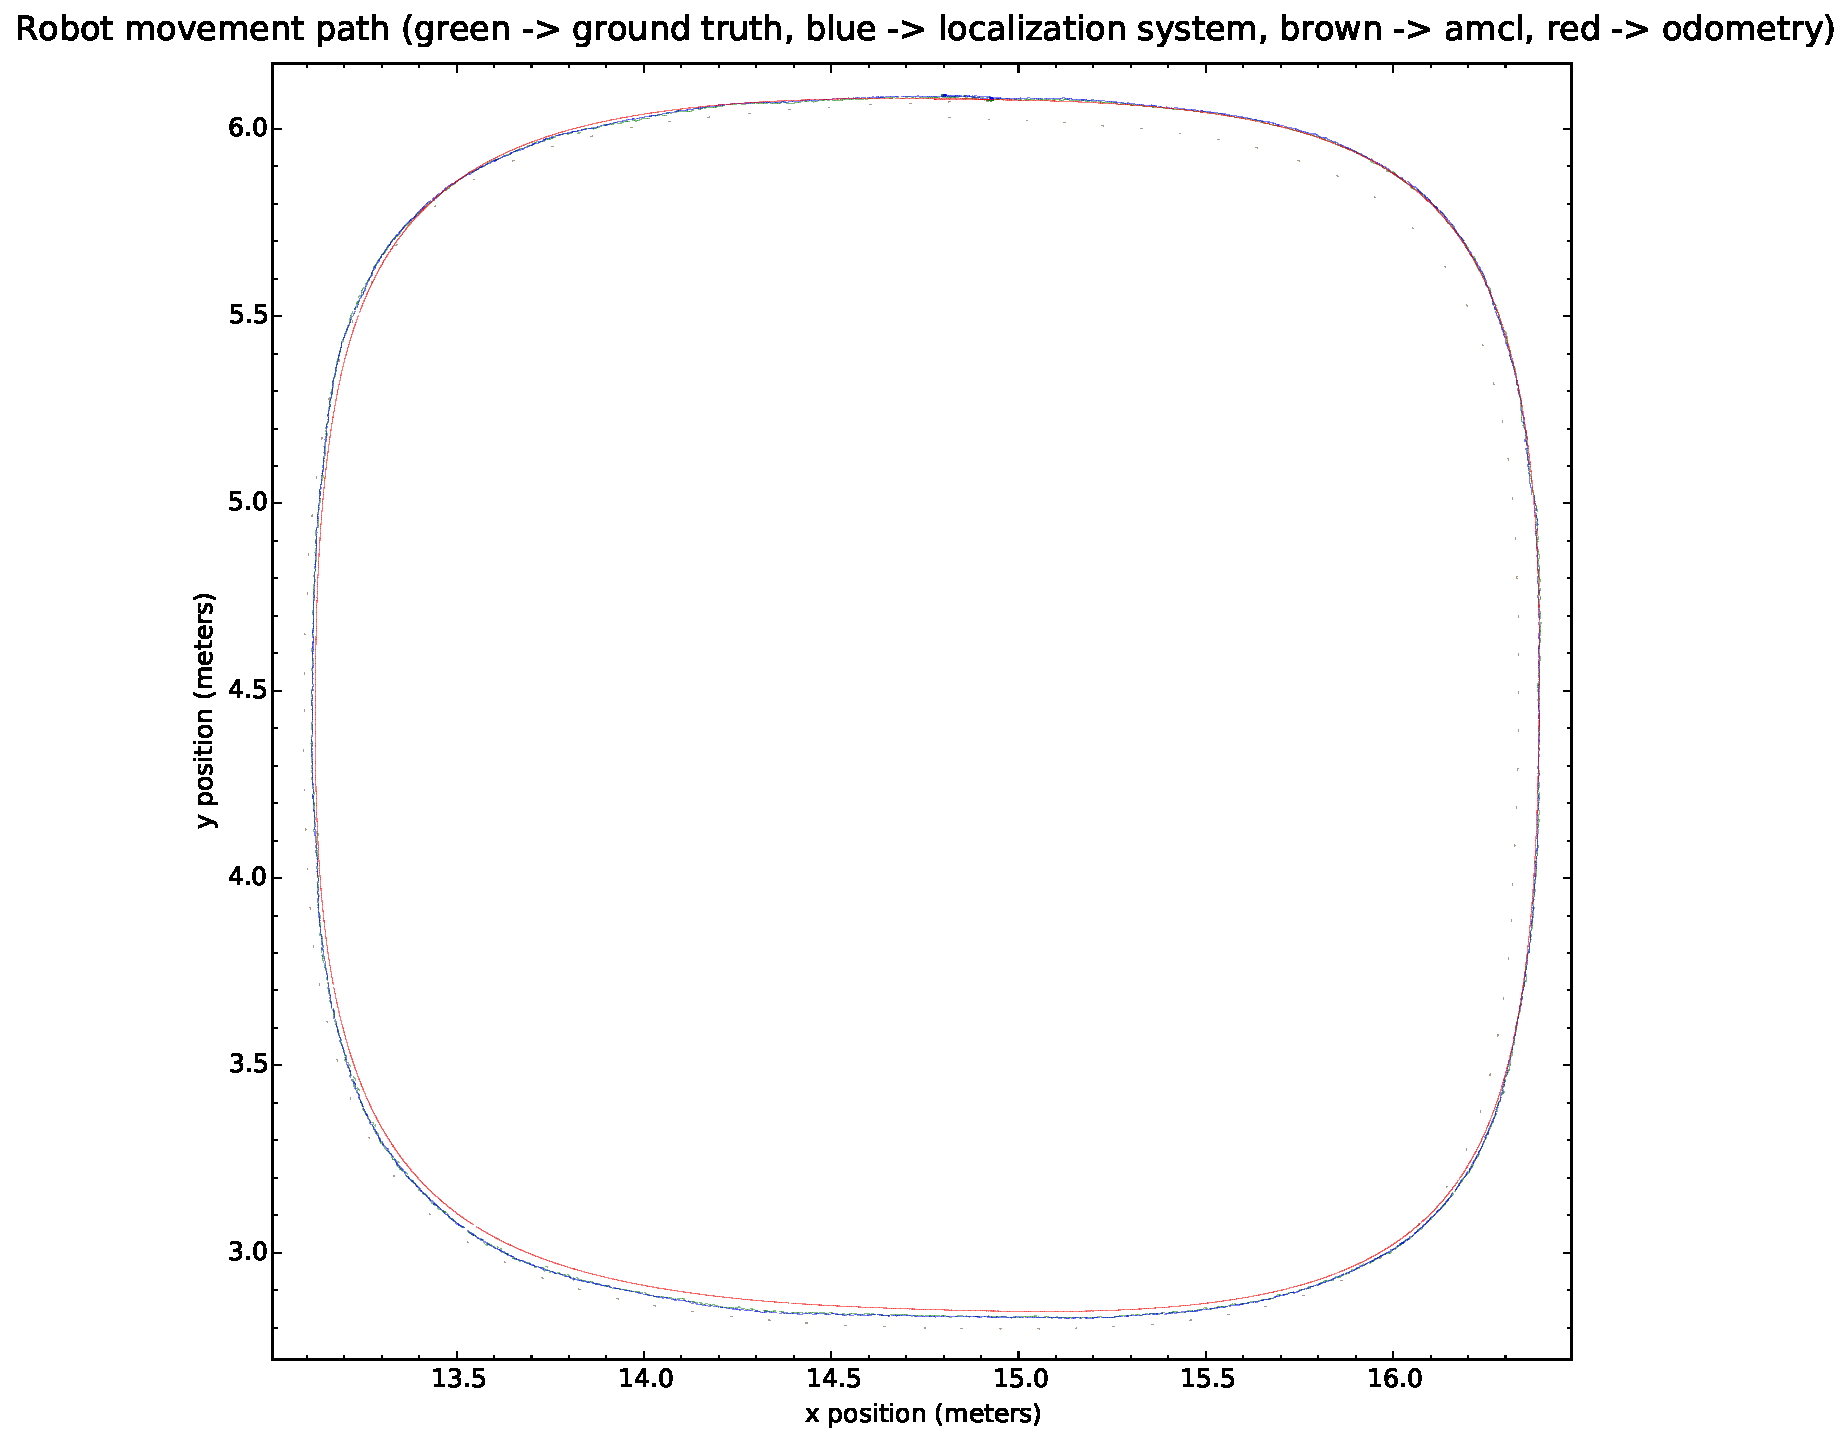
\includegraphics[width=0.8\textwidth]{appendices/tests-3dof/jarvis-robot/\currfilebase/graphs/robot-movement-path-with-odometry-and-amcl}
	\caption{Poses estimated by the ground truth, localization system, \glsentrytext{amcl} and odometry}
\end{figure}

\begin{figure}[H]
	\centering
	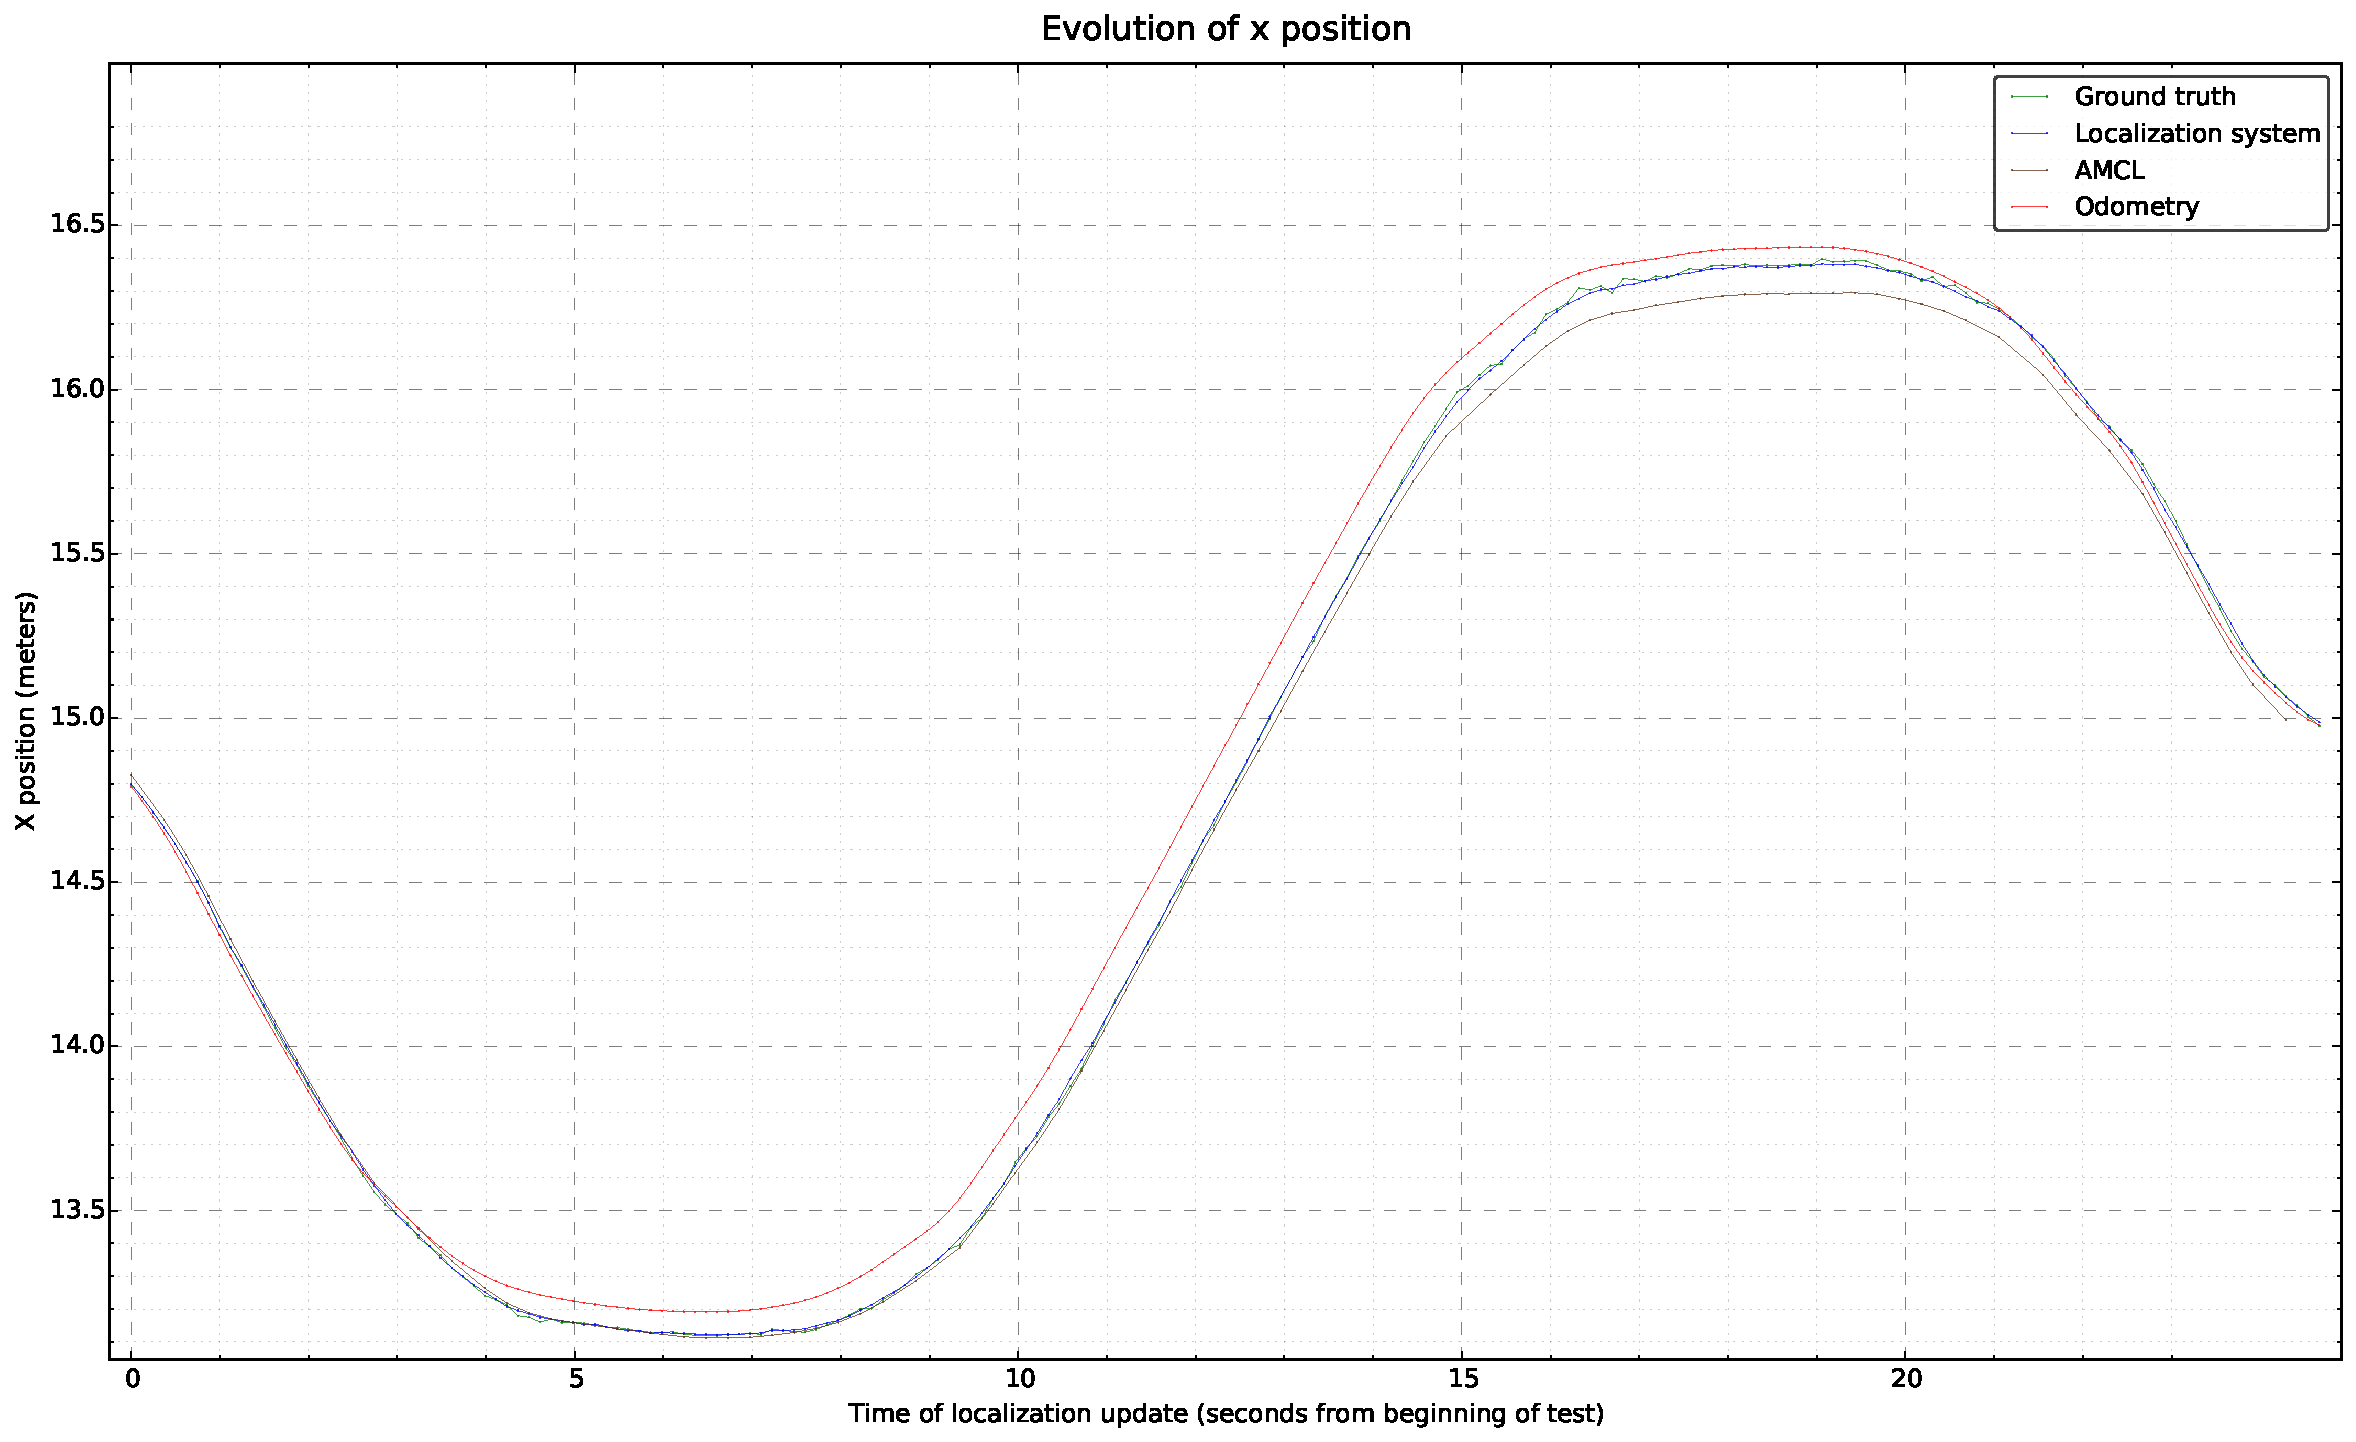
\includegraphics[width=0.53\textwidth]{appendices/tests-3dof/jarvis-robot/\currfilebase/graphs/robot-movement-path-position-evolution-x-with-amcl}
	\caption{Evolution of x position over time}
\end{figure}

\begin{figure}[H]
	\centering
	\includegraphics[width=0.53\textwidth]{appendices/tests-3dof/jarvis-robot/\currfilebase/graphs/robot-movement-path-position-evolution-y-with-amcl}
	\caption{Evolution of y position over time}
\end{figure}


%Distance derivatives
\begin{figure}[H]
	\centering
	\includegraphics[width=0.7\textwidth]{appendices/tests-3dof/jarvis-robot/\currfilebase/graphs/robot-movement-path-position-differences-with-amcl}
	\caption{Distance traveled between consecutive pose estimations}
\end{figure}

\begin{figure}[H]
	\centering
	\includegraphics[width=0.7\textwidth]{appendices/tests-3dof/jarvis-robot/\currfilebase/graphs/robot-movement-path-linear-velocity-with-amcl}
	\caption{Estimated linear velocity}
\end{figure}

\begin{figure}[H]
	\centering
	\includegraphics[width=0.7\textwidth]{appendices/tests-3dof/jarvis-robot/\currfilebase/graphs/robot-movement-path-linear-acceleration-with-amcl}
	\caption{Estimated linear acceleration}
\end{figure}


%Angular derivatives
\begin{figure}[H]
	\centering
	\includegraphics[width=0.69\textwidth]{appendices/tests-3dof/jarvis-robot/\currfilebase/graphs/robot-movement-path-angular-differences-with-amcl}
	\caption{Angular differences between consecutive pose estimations}
\end{figure}

\begin{figure}[H]
	\centering
	\includegraphics[width=0.69\textwidth]{appendices/tests-3dof/jarvis-robot/\currfilebase/graphs/robot-movement-path-angular-velocity-with-amcl}
	\caption{Estimated angular velocity}
\end{figure}

\begin{figure}[H]
	\centering
	\includegraphics[width=0.69\textwidth]{appendices/tests-3dof/jarvis-robot/\currfilebase/graphs/robot-movement-path-angular-acceleration-with-amcl}
	\caption{Estimated angular acceleration}
\end{figure}


%Translation errors
\begin{figure}[H]
	\centering
	\includegraphics[width=0.69\textwidth]{appendices/tests-3dof/jarvis-robot/\currfilebase/graphs/odometry-translation-error-millimeters}
	\caption{Odometry translation errors}
\end{figure}

\begin{figure}[H]
	\centering
	\includegraphics[width=0.69\textwidth]{appendices/tests-3dof/jarvis-robot/\currfilebase/graphs/translation-error-millimeters}
	\caption{Localization system translation errors}
\end{figure}

\begin{figure}[H]
	\centering
	\includegraphics[width=0.69\textwidth]{appendices/tests-3dof/jarvis-robot/\currfilebase/graphs/translation-error-millimeters-amcl}
	\caption{\glsentrytext{amcl} translation errors}
\end{figure}


%Translation errors components
\begin{figure}[H]
	\centering
	\includegraphics[width=0.69\textwidth]{appendices/tests-3dof/jarvis-robot/\currfilebase/graphs/odometry-translation-error-components-millimeters}
	\caption{Odometry translation errors components}
\end{figure}

\begin{figure}[H]
	\centering
	\includegraphics[width=0.69\textwidth]{appendices/tests-3dof/jarvis-robot/\currfilebase/graphs/translation-error-components-millimeters}
	\caption{Localization system translation errors components}
\end{figure}

\begin{figure}[H]
	\centering
	\includegraphics[width=0.69\textwidth]{appendices/tests-3dof/jarvis-robot/\currfilebase/graphs/translation-error-components-millimeters-amcl}
	\caption{\glsentrytext{amcl} translation errors components}
\end{figure}


%Translation errors distributions
\begin{figure}[H]
	\centering
	\includegraphics[width=0.73\textwidth]{appendices/tests-3dof/jarvis-robot/\currfilebase/graphs/odometry-translation-error-millimeters-distributions}
	\caption{Probability distributions for the odometry translation errors}
\end{figure}

\begin{figure}[H]
	\centering
	\includegraphics[width=0.73\textwidth]{appendices/tests-3dof/jarvis-robot/\currfilebase/graphs/translation-error-millimeters-distributions}
	\caption{Probability distributions for the localization system translation errors}
\end{figure}

\begin{figure}[H]
	\centering
	\includegraphics[width=0.73\textwidth]{appendices/tests-3dof/jarvis-robot/\currfilebase/graphs/translation-error-millimeters-distributions-amcl}
	\caption{Probability distributions for the \glsentrytext{amcl} translation errors}
\end{figure}


%Angular errors axis
\begin{figure}[H]
	\centering
	\includegraphics[width=0.7\textwidth]{appendices/tests-3dof/jarvis-robot/\currfilebase/graphs/odometry-rotation-error-axis}
	\caption{Odometry rotation errors axis}
\end{figure}

\begin{figure}[H]
	\centering
	\includegraphics[width=0.7\textwidth]{appendices/tests-3dof/jarvis-robot/\currfilebase/graphs/rotation-error-axis}
	\caption{Localization system rotation errors axis}
\end{figure}

\begin{figure}[H]
	\centering
	\includegraphics[width=0.7\textwidth]{appendices/tests-3dof/jarvis-robot/\currfilebase/graphs/rotation-error-axis-amcl}
	\caption{\glsentrytext{amcl} rotation errors axis}
\end{figure}


%Angular errors
\begin{figure}[H]
	\centering
	\includegraphics[width=0.69\textwidth]{appendices/tests-3dof/jarvis-robot/\currfilebase/graphs/odometry-rotation-error-degrees}
	\caption{Odometry rotation errors}
\end{figure}

\begin{figure}[H]
	\centering
	\includegraphics[width=0.69\textwidth]{appendices/tests-3dof/jarvis-robot/\currfilebase/graphs/rotation-error-degrees}
	\caption{Localization system rotation errors}
\end{figure}

\begin{figure}[H]
	\centering
	\includegraphics[width=0.69\textwidth]{appendices/tests-3dof/jarvis-robot/\currfilebase/graphs/rotation-error-degrees-amcl}
	\caption{\glsentrytext{amcl} rotation errors}
\end{figure}


%Angular errors distributions
\begin{figure}[H]
	\centering
	\includegraphics[width=0.73\textwidth]{appendices/tests-3dof/jarvis-robot/\currfilebase/graphs/odometry-rotation-error-degrees-distributions}
	\caption{Probability distributions for the odometry rotation errors}
\end{figure}

\begin{figure}[H]
	\centering
	\includegraphics[width=0.73\textwidth]{appendices/tests-3dof/jarvis-robot/\currfilebase/graphs/rotation-error-degrees-distributions}
	\caption{Probability distributions for the localization system rotation errors}
\end{figure}

\begin{figure}[H]
	\centering
	\includegraphics[width=0.73\textwidth]{appendices/tests-3dof/jarvis-robot/\currfilebase/graphs/rotation-error-degrees-distributions-amcl}
	\caption{Probability distributions for the \glsentrytext{amcl} rotation errors}
\end{figure}


%Translation corrections
\begin{figure}[H]
	\centering
	\includegraphics[width=0.69\textwidth]{appendices/tests-3dof/jarvis-robot/\currfilebase/graphs/translation-correction-millimeters}
	\caption{Translation corrections performed by the localization system}
\end{figure}

\begin{figure}[H]
	\centering
	\includegraphics[width=0.69\textwidth]{appendices/tests-3dof/jarvis-robot/\currfilebase/graphs/translation-corrections-components-millimeters}
	\caption{Translation corrections components performed by the localization system}
\end{figure}

\begin{figure}[H]
	\centering
	\includegraphics[width=0.69\textwidth]{appendices/tests-3dof/jarvis-robot/\currfilebase/graphs/translation-correction-millimeters-distributions}
	\caption{Probability distributions for the translation corrections performed by the localization system}
\end{figure}


%Rotation corrections axis
\begin{figure}[H]
	\centering
	\includegraphics[width=0.69\textwidth]{appendices/tests-3dof/jarvis-robot/\currfilebase/graphs/rotation-correction-axis}
	\caption{Rotation corrections (axis) performed by the localization system}
\end{figure}

\begin{figure}[H]
	\centering
	\includegraphics[width=0.69\textwidth]{appendices/tests-3dof/jarvis-robot/\currfilebase/graphs/rotation-correction-degrees}
	\caption{Rotation corrections performed by the localization system}
\end{figure}

\begin{figure}[H]
	\centering
	\includegraphics[width=0.69\textwidth]{appendices/tests-3dof/jarvis-robot/\currfilebase/graphs/rotation-correction-degrees-distributions}
	\caption{Probability distributions for the rotation corrections performed by the localization system}
\end{figure}


%Registered points (inliers / outliers)
\begin{figure}[H]
	\centering
	\includegraphics[width=0.71\textwidth]{appendices/tests-3dof/jarvis-robot/\currfilebase/graphs/pointclouds-size}
	\caption{Point clouds size in several of the localization system processing stages}
\end{figure}

\begin{figure}[H]
	\centering
	\includegraphics[width=0.71\textwidth]{appendices/tests-3dof/jarvis-robot/\currfilebase/graphs/registered-points}
	\caption{Number of registered points}
\end{figure}

\begin{figure}[H]
	\centering
	\includegraphics[width=0.71\textwidth]{appendices/tests-3dof/jarvis-robot/\currfilebase/graphs/outlier-percentage-distributions}
	\caption{Probability distributions for the ambient point cloud outlier percentage}
\end{figure}


\begin{figure}[H]
	\centering
	\includegraphics[width=0.7\textwidth]{appendices/tests-3dof/jarvis-robot/\currfilebase/graphs/registered-points-angular-distribution}
	\caption{Angular distribution percentage of registered points}
\end{figure}

\begin{figure}[H]
	\centering
	\includegraphics[width=0.7\textwidth]{appendices/tests-3dof/jarvis-robot/\currfilebase/graphs/root-mean-square-error-inliers}
	\caption{Root Mean Square Error of the inliers}
\end{figure}

\begin{figure}[H]
	\centering
	\includegraphics[width=0.7\textwidth]{appendices/tests-3dof/jarvis-robot/\currfilebase/graphs/root-mean-square-error-inliers-distributions}
	\caption{Probability distributions for the Root Mean Square Error of the inliers}
\end{figure}


%Computation times
\begin{figure}[H]
	\centering
	\includegraphics[width=0.72\textwidth]{appendices/tests-3dof/jarvis-robot/\currfilebase/graphs/computation-times-milliseconds}
	\caption{Localization system computation times}
\end{figure}

\begin{figure}[H]
	\centering
	\includegraphics[width=0.72\textwidth]{appendices/tests-3dof/jarvis-robot/\currfilebase/graphs/computation-times-milliseconds-pointcloud-registration-time-distributions}
	\caption{Probability distributions for the point cloud registration time}
\end{figure}

\begin{figure}[H]
	\centering
	\includegraphics[width=0.72\textwidth]{appendices/tests-3dof/jarvis-robot/\currfilebase/graphs/computation-times-milliseconds-global-time-distributions}
	\caption{Probability distributions for the localization system global computation time}
\end{figure}

\subsection{Complex path using the Jarvis robot at 5 cm/s}\label{subsec:appendix-a_jarvis-robot-tests_complex-path-using-the-jarvis-robot-at-5-cm-s}

The figures in this section show the detailed results of the Jarvis robot with a 10 mm resolution map in the RoboCup field following a complex path and moving at 5 cm/s.


%Animated paths
\begin{figure}[H]
	\centering
	\animategraphics[width=0.8\textwidth,loop,autoplay,controls]{1}{appendices/tests-3dof/jarvis-robot/\currfilebase/images-ground-truth/image}{1}{10}
	\caption{Animation of laser scans using the ground truth poses}
\end{figure}

\begin{figure}[H]
	\centering
	\animategraphics[width=0.8\textwidth,loop,autoplay,controls]{1}{appendices/tests-3dof/jarvis-robot/\currfilebase/images-drl/image}{1}{10}
	\caption{Animation of laser scans using the localization system poses}
\end{figure}

\begin{figure}[H]
	\centering
	\animategraphics[width=0.8\textwidth,loop,autoplay,controls]{1}{appendices/tests-3dof/jarvis-robot/\currfilebase/images-amcl/image}{1}{10}
	\caption{Animation of laser scans using the \glsentrytext{amcl} poses}
\end{figure}


%Laser assembly
\begin{figure}[H]
	\centering
	\includegraphics[width=0.993\textwidth]{appendices/tests-3dof/jarvis-robot/\currfilebase/ground-truth-cumulative}
	\caption{Laser scans assembled on top of the map using the ground truth poses}
\end{figure}

\begin{figure}[H]
	\centering
	\includegraphics[width=0.993\textwidth]{appendices/tests-3dof/jarvis-robot/\currfilebase/drl-cumulative}
	\caption{Laser scans assembled on top of the map using the localization system poses}
\end{figure}

\begin{figure}[H]
	\centering
	\includegraphics[width=0.993\textwidth]{appendices/tests-3dof/jarvis-robot/\currfilebase/amcl-cumulative}
	\caption{Laser scans assembled on top of the map using the \glsentrytext{amcl} poses}
\end{figure}


%Paths
\begin{figure}[H]
	\centering
	\includegraphics[width=\textwidth]{appendices/tests-3dof/jarvis-robot/\currfilebase/graphs/robot-movement-path-with-odometry-and-amcl}
	\caption{Poses estimated by the ground truth, localization system, \glsentrytext{amcl} and odometry}
\end{figure}

\begin{figure}[H]
	\centering
	\includegraphics[width=0.73\textwidth]{appendices/tests-3dof/jarvis-robot/\currfilebase/graphs/robot-movement-path-position-evolution-x-with-amcl}
	\caption{Evolution of x position over time}
\end{figure}

\begin{figure}[H]
	\centering
	\includegraphics[width=0.73\textwidth]{appendices/tests-3dof/jarvis-robot/\currfilebase/graphs/robot-movement-path-position-evolution-y-with-amcl}
	\caption{Evolution of y position over time}
\end{figure}


%Distance derivatives
\begin{figure}[H]
	\centering
	\includegraphics[width=0.7\textwidth]{appendices/tests-3dof/jarvis-robot/\currfilebase/graphs/robot-movement-path-position-differences-with-amcl}
	\caption{Distance traveled between consecutive pose estimations}
\end{figure}

\begin{figure}[H]
	\centering
	\includegraphics[width=0.7\textwidth]{appendices/tests-3dof/jarvis-robot/\currfilebase/graphs/robot-movement-path-linear-velocity-with-amcl}
	\caption{Estimated linear velocity}
\end{figure}

\begin{figure}[H]
	\centering
	\includegraphics[width=0.7\textwidth]{appendices/tests-3dof/jarvis-robot/\currfilebase/graphs/robot-movement-path-linear-acceleration-with-amcl}
	\caption{Estimated linear acceleration}
\end{figure}


%Angular derivatives
\begin{figure}[H]
	\centering
	\includegraphics[width=0.69\textwidth]{appendices/tests-3dof/jarvis-robot/\currfilebase/graphs/robot-movement-path-angular-differences-with-amcl}
	\caption{Angular differences between consecutive pose estimations}
\end{figure}

\begin{figure}[H]
	\centering
	\includegraphics[width=0.69\textwidth]{appendices/tests-3dof/jarvis-robot/\currfilebase/graphs/robot-movement-path-angular-velocity-with-amcl}
	\caption{Estimated angular velocity}
\end{figure}

\begin{figure}[H]
	\centering
	\includegraphics[width=0.69\textwidth]{appendices/tests-3dof/jarvis-robot/\currfilebase/graphs/robot-movement-path-angular-acceleration-with-amcl}
	\caption{Estimated angular acceleration}
\end{figure}


%Translation errors
\begin{figure}[H]
	\centering
	\includegraphics[width=0.69\textwidth]{appendices/tests-3dof/jarvis-robot/\currfilebase/graphs/odometry-translation-error-millimeters}
	\caption{Odometry translation errors}
\end{figure}

\begin{figure}[H]
	\centering
	\includegraphics[width=0.69\textwidth]{appendices/tests-3dof/jarvis-robot/\currfilebase/graphs/translation-error-millimeters}
	\caption{Localization system translation errors}
\end{figure}

\begin{figure}[H]
	\centering
	\includegraphics[width=0.69\textwidth]{appendices/tests-3dof/jarvis-robot/\currfilebase/graphs/translation-error-millimeters-amcl}
	\caption{\glsentrytext{amcl} translation errors}
\end{figure}


%Translation errors components
\begin{figure}[H]
	\centering
	\includegraphics[width=0.69\textwidth]{appendices/tests-3dof/jarvis-robot/\currfilebase/graphs/odometry-translation-error-components-millimeters}
	\caption{Odometry translation errors components}
\end{figure}

\begin{figure}[H]
	\centering
	\includegraphics[width=0.69\textwidth]{appendices/tests-3dof/jarvis-robot/\currfilebase/graphs/translation-error-components-millimeters}
	\caption{Localization system translation errors components}
\end{figure}

\begin{figure}[H]
	\centering
	\includegraphics[width=0.69\textwidth]{appendices/tests-3dof/jarvis-robot/\currfilebase/graphs/translation-error-components-millimeters-amcl}
	\caption{\glsentrytext{amcl} translation errors components}
\end{figure}


%Translation errors distributions
\begin{figure}[H]
	\centering
	\includegraphics[width=0.73\textwidth]{appendices/tests-3dof/jarvis-robot/\currfilebase/graphs/odometry-translation-error-millimeters-distributions}
	\caption{Probability distributions for the odometry translation errors}
\end{figure}

\begin{figure}[H]
	\centering
	\includegraphics[width=0.73\textwidth]{appendices/tests-3dof/jarvis-robot/\currfilebase/graphs/translation-error-millimeters-distributions}
	\caption{Probability distributions for the localization system translation errors}
\end{figure}

\begin{figure}[H]
	\centering
	\includegraphics[width=0.73\textwidth]{appendices/tests-3dof/jarvis-robot/\currfilebase/graphs/translation-error-millimeters-distributions-amcl}
	\caption{Probability distributions for the \glsentrytext{amcl} translation errors}
\end{figure}


%Angular errors axis
\begin{figure}[H]
	\centering
	\includegraphics[width=0.7\textwidth]{appendices/tests-3dof/jarvis-robot/\currfilebase/graphs/odometry-rotation-error-axis}
	\caption{Odometry rotation errors axis}
\end{figure}

\begin{figure}[H]
	\centering
	\includegraphics[width=0.7\textwidth]{appendices/tests-3dof/jarvis-robot/\currfilebase/graphs/rotation-error-axis}
	\caption{Localization system rotation errors axis}
\end{figure}

\begin{figure}[H]
	\centering
	\includegraphics[width=0.7\textwidth]{appendices/tests-3dof/jarvis-robot/\currfilebase/graphs/rotation-error-axis-amcl}
	\caption{\glsentrytext{amcl} rotation errors axis}
\end{figure}


%Angular errors
\begin{figure}[H]
	\centering
	\includegraphics[width=0.69\textwidth]{appendices/tests-3dof/jarvis-robot/\currfilebase/graphs/odometry-rotation-error-degrees}
	\caption{Odometry rotation errors}
\end{figure}

\begin{figure}[H]
	\centering
	\includegraphics[width=0.69\textwidth]{appendices/tests-3dof/jarvis-robot/\currfilebase/graphs/rotation-error-degrees}
	\caption{Localization system rotation errors}
\end{figure}

\begin{figure}[H]
	\centering
	\includegraphics[width=0.69\textwidth]{appendices/tests-3dof/jarvis-robot/\currfilebase/graphs/rotation-error-degrees-amcl}
	\caption{\glsentrytext{amcl} rotation errors}
\end{figure}


%Angular errors distributions
\begin{figure}[H]
	\centering
	\includegraphics[width=0.73\textwidth]{appendices/tests-3dof/jarvis-robot/\currfilebase/graphs/odometry-rotation-error-degrees-distributions}
	\caption{Probability distributions for the odometry rotation errors}
\end{figure}

\begin{figure}[H]
	\centering
	\includegraphics[width=0.73\textwidth]{appendices/tests-3dof/jarvis-robot/\currfilebase/graphs/rotation-error-degrees-distributions}
	\caption{Probability distributions for the localization system rotation errors}
\end{figure}

\begin{figure}[H]
	\centering
	\includegraphics[width=0.73\textwidth]{appendices/tests-3dof/jarvis-robot/\currfilebase/graphs/rotation-error-degrees-distributions-amcl}
	\caption{Probability distributions for the \glsentrytext{amcl} rotation errors}
\end{figure}


%Translation corrections
\begin{figure}[H]
	\centering
	\includegraphics[width=0.69\textwidth]{appendices/tests-3dof/jarvis-robot/\currfilebase/graphs/translation-correction-millimeters}
	\caption{Translation corrections performed by the localization system}
\end{figure}

\begin{figure}[H]
	\centering
	\includegraphics[width=0.69\textwidth]{appendices/tests-3dof/jarvis-robot/\currfilebase/graphs/translation-corrections-components-millimeters}
	\caption{Translation corrections components performed by the localization system}
\end{figure}

\begin{figure}[H]
	\centering
	\includegraphics[width=0.69\textwidth]{appendices/tests-3dof/jarvis-robot/\currfilebase/graphs/translation-correction-millimeters-distributions}
	\caption{Probability distributions for the translation corrections performed by the localization system}
\end{figure}


%Rotation corrections axis
\begin{figure}[H]
	\centering
	\includegraphics[width=0.69\textwidth]{appendices/tests-3dof/jarvis-robot/\currfilebase/graphs/rotation-correction-axis}
	\caption{Rotation corrections (axis) performed by the localization system}
\end{figure}

\begin{figure}[H]
	\centering
	\includegraphics[width=0.69\textwidth]{appendices/tests-3dof/jarvis-robot/\currfilebase/graphs/rotation-correction-degrees}
	\caption{Rotation corrections performed by the localization system}
\end{figure}

\begin{figure}[H]
	\centering
	\includegraphics[width=0.69\textwidth]{appendices/tests-3dof/jarvis-robot/\currfilebase/graphs/rotation-correction-degrees-distributions}
	\caption{Probability distributions for the rotation corrections performed by the localization system}
\end{figure}


%Registered points (inliers / outliers)
\begin{figure}[H]
	\centering
	\includegraphics[width=0.71\textwidth]{appendices/tests-3dof/jarvis-robot/\currfilebase/graphs/pointclouds-size}
	\caption{Point clouds size in several of the localization system processing stages}
\end{figure}

\begin{figure}[H]
	\centering
	\includegraphics[width=0.71\textwidth]{appendices/tests-3dof/jarvis-robot/\currfilebase/graphs/registered-points}
	\caption{Number of registered points}
\end{figure}

\begin{figure}[H]
	\centering
	\includegraphics[width=0.71\textwidth]{appendices/tests-3dof/jarvis-robot/\currfilebase/graphs/outlier-percentage-distributions}
	\caption{Probability distributions for the ambient point cloud outlier percentage}
\end{figure}


\begin{figure}[H]
	\centering
	\includegraphics[width=0.71\textwidth]{appendices/tests-3dof/jarvis-robot/\currfilebase/graphs/registered-points-angular-distribution}
	\caption{Angular distribution percentage of registered points}
\end{figure}

\begin{figure}[H]
	\centering
	\includegraphics[width=0.71\textwidth]{appendices/tests-3dof/jarvis-robot/\currfilebase/graphs/root-mean-square-error-inliers}
	\caption{Root Mean Square Error of the inliers}
\end{figure}

\begin{figure}[H]
	\centering
	\includegraphics[width=0.71\textwidth]{appendices/tests-3dof/jarvis-robot/\currfilebase/graphs/root-mean-square-error-inliers-distributions}
	\caption{Probability distributions for the Root Mean Square Error of the inliers}
\end{figure}


%Computation times
\begin{figure}[H]
	\centering
	\includegraphics[width=0.72\textwidth]{appendices/tests-3dof/jarvis-robot/\currfilebase/graphs/computation-times-milliseconds}
	\caption{Localization system computation times}
\end{figure}

\begin{figure}[H]
	\centering
	\includegraphics[width=0.72\textwidth]{appendices/tests-3dof/jarvis-robot/\currfilebase/graphs/computation-times-milliseconds-pointcloud-registration-time-distributions}
	\caption{Probability distributions for the point cloud registration time}
\end{figure}

\begin{figure}[H]
	\centering
	\includegraphics[width=0.72\textwidth]{appendices/tests-3dof/jarvis-robot/\currfilebase/graphs/computation-times-milliseconds-global-time-distributions}
	\caption{Probability distributions for the localization system global computation time}
\end{figure}

\subsection{Complex path using the Jarvis robot at 50-30-50-10 cm/s}\label{subsec:appendix-a_jarvis-robot-tests_complex-path-using-the-jarvis-robot-at-50-30-50-10-cm-s}

The figures in this section show the detailed results of the Jarvis robot with a 10 mm resolution map in the RoboCup field following a complex path and moving at 50-30-50-10 cm/s.


%Animated paths
\begin{figure}[H]
	\centering
	\animategraphics[width=0.8\textwidth,loop,autoplay,controls]{1}{appendices/tests-3dof/jarvis-robot/\currfilebase/images-ground-truth/image}{1}{60}
	\caption{Animation of laser scans using the ground truth poses}
\end{figure}

\begin{figure}[H]
	\centering
	\animategraphics[width=0.8\textwidth,loop,autoplay,controls]{1}{appendices/tests-3dof/jarvis-robot/\currfilebase/images-drl/image}{1}{60}
	\caption{Animation of laser scans using the localization system poses}
\end{figure}

\begin{figure}[H]
	\centering
	\animategraphics[width=0.8\textwidth,loop,autoplay,controls]{1}{appendices/tests-3dof/jarvis-robot/\currfilebase/images-amcl/image}{1}{60}
	\caption{Animation of laser scans using the \glsentrytext{amcl} poses}
\end{figure}


%Laser assembly
\begin{figure}[H]
	\centering
	\includegraphics[width=0.993\textwidth]{appendices/tests-3dof/jarvis-robot/\currfilebase/ground-truth-cumulative}
	\caption{Laser scans assembled on top of the map using the ground truth poses}
\end{figure}

\begin{figure}[H]
	\centering
	\includegraphics[width=0.993\textwidth]{appendices/tests-3dof/jarvis-robot/\currfilebase/drl-cumulative}
	\caption{Laser scans assembled on top of the map using the localization system poses}
\end{figure}

\begin{figure}[H]
	\centering
	\includegraphics[width=0.993\textwidth]{appendices/tests-3dof/jarvis-robot/\currfilebase/amcl-cumulative}
	\caption{Laser scans assembled on top of the map using the \glsentrytext{amcl} poses}
\end{figure}


%Paths
\begin{figure}[H]
	\centering
	\includegraphics[width=\textwidth]{appendices/tests-3dof/jarvis-robot/\currfilebase/graphs/robot-movement-path-with-odometry-and-amcl}
	\caption{Poses estimated by the ground truth, localization system, \glsentrytext{amcl} and odometry}
\end{figure}

\begin{figure}[H]
	\centering
	\includegraphics[width=0.7\textwidth]{appendices/tests-3dof/jarvis-robot/\currfilebase/graphs/robot-movement-path-position-evolution-x-with-amcl}
	\caption{Evolution of x position over time}
\end{figure}

\begin{figure}[H]
	\centering
	\includegraphics[width=0.7\textwidth]{appendices/tests-3dof/jarvis-robot/\currfilebase/graphs/robot-movement-path-position-evolution-y-with-amcl}
	\caption{Evolution of y position over time}
\end{figure}


%Distance derivatives
\begin{figure}[H]
	\centering
	\includegraphics[width=0.7\textwidth]{appendices/tests-3dof/jarvis-robot/\currfilebase/graphs/robot-movement-path-position-differences-with-amcl}
	\caption{Distance traveled between consecutive pose estimations}
\end{figure}

\begin{figure}[H]
	\centering
	\includegraphics[width=0.7\textwidth]{appendices/tests-3dof/jarvis-robot/\currfilebase/graphs/robot-movement-path-linear-velocity-with-amcl}
	\caption{Estimated linear velocity}
\end{figure}

\begin{figure}[H]
	\centering
	\includegraphics[width=0.7\textwidth]{appendices/tests-3dof/jarvis-robot/\currfilebase/graphs/robot-movement-path-linear-acceleration-with-amcl}
	\caption{Estimated linear acceleration}
\end{figure}


%Angular derivatives
\begin{figure}[H]
	\centering
	\includegraphics[width=0.69\textwidth]{appendices/tests-3dof/jarvis-robot/\currfilebase/graphs/robot-movement-path-angular-differences-with-amcl}
	\caption{Angular differences between consecutive pose estimations}
\end{figure}

\begin{figure}[H]
	\centering
	\includegraphics[width=0.69\textwidth]{appendices/tests-3dof/jarvis-robot/\currfilebase/graphs/robot-movement-path-angular-velocity-with-amcl}
	\caption{Estimated angular velocity}
\end{figure}

\begin{figure}[H]
	\centering
	\includegraphics[width=0.69\textwidth]{appendices/tests-3dof/jarvis-robot/\currfilebase/graphs/robot-movement-path-angular-acceleration-with-amcl}
	\caption{Estimated angular acceleration}
\end{figure}


%Translation errors
\begin{figure}[H]
	\centering
	\includegraphics[width=0.69\textwidth]{appendices/tests-3dof/jarvis-robot/\currfilebase/graphs/odometry-translation-error-millimeters}
	\caption{Odometry translation errors}
\end{figure}

\begin{figure}[H]
	\centering
	\includegraphics[width=0.69\textwidth]{appendices/tests-3dof/jarvis-robot/\currfilebase/graphs/translation-error-millimeters}
	\caption{Localization system translation errors}
\end{figure}

\begin{figure}[H]
	\centering
	\includegraphics[width=0.69\textwidth]{appendices/tests-3dof/jarvis-robot/\currfilebase/graphs/translation-error-millimeters-amcl}
	\caption{\glsentrytext{amcl} translation errors}
\end{figure}


%Translation errors components
\begin{figure}[H]
	\centering
	\includegraphics[width=0.69\textwidth]{appendices/tests-3dof/jarvis-robot/\currfilebase/graphs/odometry-translation-error-components-millimeters}
	\caption{Odometry translation errors components}
\end{figure}

\begin{figure}[H]
	\centering
	\includegraphics[width=0.69\textwidth]{appendices/tests-3dof/jarvis-robot/\currfilebase/graphs/translation-error-components-millimeters}
	\caption{Localization system translation errors components}
\end{figure}

\begin{figure}[H]
	\centering
	\includegraphics[width=0.69\textwidth]{appendices/tests-3dof/jarvis-robot/\currfilebase/graphs/translation-error-components-millimeters-amcl}
	\caption{\glsentrytext{amcl} translation errors components}
\end{figure}


%Translation errors distributions
\begin{figure}[H]
	\centering
	\includegraphics[width=0.73\textwidth]{appendices/tests-3dof/jarvis-robot/\currfilebase/graphs/odometry-translation-error-millimeters-distributions}
	\caption{Probability distributions for the odometry translation errors}
\end{figure}

\begin{figure}[H]
	\centering
	\includegraphics[width=0.73\textwidth]{appendices/tests-3dof/jarvis-robot/\currfilebase/graphs/translation-error-millimeters-distributions}
	\caption{Probability distributions for the localization system translation errors}
\end{figure}

\begin{figure}[H]
	\centering
	\includegraphics[width=0.73\textwidth]{appendices/tests-3dof/jarvis-robot/\currfilebase/graphs/translation-error-millimeters-distributions-amcl}
	\caption{Probability distributions for the \glsentrytext{amcl} translation errors}
\end{figure}


%Angular errors axis
\begin{figure}[H]
	\centering
	\includegraphics[width=0.7\textwidth]{appendices/tests-3dof/jarvis-robot/\currfilebase/graphs/odometry-rotation-error-axis}
	\caption{Odometry rotation errors axis}
\end{figure}

\begin{figure}[H]
	\centering
	\includegraphics[width=0.7\textwidth]{appendices/tests-3dof/jarvis-robot/\currfilebase/graphs/rotation-error-axis}
	\caption{Localization system rotation errors axis}
\end{figure}

\begin{figure}[H]
	\centering
	\includegraphics[width=0.7\textwidth]{appendices/tests-3dof/jarvis-robot/\currfilebase/graphs/rotation-error-axis-amcl}
	\caption{\glsentrytext{amcl} rotation errors axis}
\end{figure}


%Angular errors
\begin{figure}[H]
	\centering
	\includegraphics[width=0.69\textwidth]{appendices/tests-3dof/jarvis-robot/\currfilebase/graphs/odometry-rotation-error-degrees}
	\caption{Odometry rotation errors}
\end{figure}

\begin{figure}[H]
	\centering
	\includegraphics[width=0.69\textwidth]{appendices/tests-3dof/jarvis-robot/\currfilebase/graphs/rotation-error-degrees}
	\caption{Localization system rotation errors}
\end{figure}

\begin{figure}[H]
	\centering
	\includegraphics[width=0.69\textwidth]{appendices/tests-3dof/jarvis-robot/\currfilebase/graphs/rotation-error-degrees-amcl}
	\caption{\glsentrytext{amcl} rotation errors}
\end{figure}


%Angular errors distributions
\begin{figure}[H]
	\centering
	\includegraphics[width=0.73\textwidth]{appendices/tests-3dof/jarvis-robot/\currfilebase/graphs/odometry-rotation-error-degrees-distributions}
	\caption{Probability distributions for the odometry rotation errors}
\end{figure}

\begin{figure}[H]
	\centering
	\includegraphics[width=0.73\textwidth]{appendices/tests-3dof/jarvis-robot/\currfilebase/graphs/rotation-error-degrees-distributions}
	\caption{Probability distributions for the localization system rotation errors}
\end{figure}

\begin{figure}[H]
	\centering
	\includegraphics[width=0.73\textwidth]{appendices/tests-3dof/jarvis-robot/\currfilebase/graphs/rotation-error-degrees-distributions-amcl}
	\caption{Probability distributions for the \glsentrytext{amcl} rotation errors}
\end{figure}


%Translation corrections
\begin{figure}[H]
	\centering
	\includegraphics[width=0.69\textwidth]{appendices/tests-3dof/jarvis-robot/\currfilebase/graphs/translation-correction-millimeters}
	\caption{Translation corrections performed by the localization system}
\end{figure}

\begin{figure}[H]
	\centering
	\includegraphics[width=0.69\textwidth]{appendices/tests-3dof/jarvis-robot/\currfilebase/graphs/translation-corrections-components-millimeters}
	\caption{Translation corrections components performed by the localization system}
\end{figure}

\begin{figure}[H]
	\centering
	\includegraphics[width=0.69\textwidth]{appendices/tests-3dof/jarvis-robot/\currfilebase/graphs/translation-correction-millimeters-distributions}
	\caption{Probability distributions for the translation corrections performed by the localization system}
\end{figure}


%Rotation corrections axis
\begin{figure}[H]
	\centering
	\includegraphics[width=0.69\textwidth]{appendices/tests-3dof/jarvis-robot/\currfilebase/graphs/rotation-correction-axis}
	\caption{Rotation corrections (axis) performed by the localization system}
\end{figure}

\begin{figure}[H]
	\centering
	\includegraphics[width=0.69\textwidth]{appendices/tests-3dof/jarvis-robot/\currfilebase/graphs/rotation-correction-degrees}
	\caption{Rotation corrections performed by the localization system}
\end{figure}

\begin{figure}[H]
	\centering
	\includegraphics[width=0.69\textwidth]{appendices/tests-3dof/jarvis-robot/\currfilebase/graphs/rotation-correction-degrees-distributions}
	\caption{Probability distributions for the rotation corrections performed by the localization system}
\end{figure}


%Registered points (inliers / outliers)
\begin{figure}[H]
	\centering
	\includegraphics[width=0.71\textwidth]{appendices/tests-3dof/jarvis-robot/\currfilebase/graphs/pointclouds-size}
	\caption{Point clouds size in several of the localization system processing stages}
\end{figure}

\begin{figure}[H]
	\centering
	\includegraphics[width=0.71\textwidth]{appendices/tests-3dof/jarvis-robot/\currfilebase/graphs/registered-points}
	\caption{Number of registered points}
\end{figure}

\begin{figure}[H]
	\centering
	\includegraphics[width=0.71\textwidth]{appendices/tests-3dof/jarvis-robot/\currfilebase/graphs/outlier-percentage-distributions}
	\caption{Probability distributions for the ambient point cloud outlier percentage}
\end{figure}


\begin{figure}[H]
	\centering
	\includegraphics[width=0.7\textwidth]{appendices/tests-3dof/jarvis-robot/\currfilebase/graphs/registered-points-angular-distribution}
	\caption{Angular distribution percentage of registered points}
\end{figure}

\begin{figure}[H]
	\centering
	\includegraphics[width=0.7\textwidth]{appendices/tests-3dof/jarvis-robot/\currfilebase/graphs/root-mean-square-error-inliers}
	\caption{Root Mean Square Error of the inliers}
\end{figure}

\begin{figure}[H]
	\centering
	\includegraphics[width=0.7\textwidth]{appendices/tests-3dof/jarvis-robot/\currfilebase/graphs/root-mean-square-error-inliers-distributions}
	\caption{Probability distributions for the Root Mean Square Error of the inliers}
\end{figure}


%Computation times
\begin{figure}[H]
	\centering
	\includegraphics[width=0.72\textwidth]{appendices/tests-3dof/jarvis-robot/\currfilebase/graphs/computation-times-milliseconds}
	\caption{Localization system computation times}
\end{figure}

\begin{figure}[H]
	\centering
	\includegraphics[width=0.72\textwidth]{appendices/tests-3dof/jarvis-robot/\currfilebase/graphs/computation-times-milliseconds-pointcloud-registration-time-distributions}
	\caption{Probability distributions for the point cloud registration time}
\end{figure}

\begin{figure}[H]
	\centering
	\includegraphics[width=0.72\textwidth]{appendices/tests-3dof/jarvis-robot/\currfilebase/graphs/computation-times-milliseconds-global-time-distributions}
	\caption{Probability distributions for the localization system global computation time}
\end{figure}

\subsection{Complex path using the Jarvis robot at 5 cm/s without laser spherical linear interpolation}\label{subsec:appendix-a_jarvis-robot-tests_complex-path-using-the-jarvis-robot-at-5-cm-s-without-laser-spherical-linear-interpolation}

The figures in this section show the results of a test performed with same configurations as the previous section, but now without using laser spherical linear interpolation.


%Animated paths
\begin{figure}[H]
	\centering
	\animategraphics[width=\textwidth,loop,autoplay,controls]{1}{appendices/tests-3dof/jarvis-robot/complex-path-with-outliers-5cm-per-sec-velocity-1-4-scans/images-drl/image}{1}{10}
	\caption{Laser scans from previous test using laser spherical linear interpolation}
\end{figure}

\begin{figure}[H]
	\centering
	\animategraphics[width=\textwidth,loop,autoplay,controls]{1}{appendices/tests-3dof/jarvis-robot/\currfilebase/images-drl/image}{1}{10}
	\caption{Laser scans without using laser spherical linear interpolation}
\end{figure}


%Laser assembly
\begin{figure}[H]
	\centering
	\includegraphics[width=0.99\textwidth]{appendices/tests-3dof/jarvis-robot/complex-path-with-outliers-5cm-per-sec-velocity-1-4-scans/drl-cumulative}
	\caption{Laser scans assembled in the previous test using laser spherical linear interpolation}
\end{figure}

\begin{figure}[H]
	\centering
	\includegraphics[width=0.99\textwidth]{appendices/tests-3dof/jarvis-robot/\currfilebase/drl-cumulative}
	\caption{Laser scans assembled without using laser spherical linear interpolation}
\end{figure}



%Paths
\begin{figure}[H]
	\centering
	\includegraphics[width=\textwidth]{appendices/tests-3dof/jarvis-robot/\currfilebase/graphs/robot-movement-path-with-odometry}
	\caption{Poses estimated by the ground truth, localization system and odometry}
\end{figure}

\begin{figure}[H]
	\centering
	\includegraphics[width=\textwidth]{appendices/tests-3dof/jarvis-robot/\currfilebase/graphs/robot-movement-path-position-evolution-x}
	\caption{Evolution of x position over time}
\end{figure}

\begin{figure}[H]
	\centering
	\includegraphics[width=\textwidth]{appendices/tests-3dof/jarvis-robot/\currfilebase/graphs/robot-movement-path-position-evolution-y}
	\caption{Evolution of y position over time}
\end{figure}


%Distance derivatives
\begin{figure}[H]
	\centering
	\includegraphics[width=\textwidth]{appendices/tests-3dof/jarvis-robot/\currfilebase/graphs/robot-movement-path-position-differences}
	\caption{Distance traveled between consecutive pose estimations}
\end{figure}


%Angular derivatives
\begin{figure}[H]
	\centering
	\includegraphics[width=\textwidth]{appendices/tests-3dof/jarvis-robot/\currfilebase/graphs/robot-movement-path-angular-differences}
	\caption{Angular differences between consecutive pose estimations}
\end{figure}


%Translation errors
\begin{figure}[H]
	\centering
	\includegraphics[width=0.69\textwidth]{appendices/tests-3dof/jarvis-robot/\currfilebase/graphs/translation-error-millimeters}
	\caption{Localization system translation errors}
\end{figure}


%Translation errors components
\begin{figure}[H]
	\centering
	\includegraphics[width=0.69\textwidth]{appendices/tests-3dof/jarvis-robot/\currfilebase/graphs/translation-error-components-millimeters}
	\caption{Localization system translation errors components}
\end{figure}


%Translation errors distributions
\begin{figure}[H]
	\centering
	\includegraphics[width=0.73\textwidth]{appendices/tests-3dof/jarvis-robot/\currfilebase/graphs/translation-error-millimeters-distributions}
	\caption{Probability distributions for the localization system translation errors}
\end{figure}



%Angular errors axis
\begin{figure}[H]
	\centering
	\includegraphics[width=0.71\textwidth]{appendices/tests-3dof/jarvis-robot/\currfilebase/graphs/rotation-error-axis}
	\caption{Localization system rotation errors axis}
\end{figure}


%Angular errors
\begin{figure}[H]
	\centering
	\includegraphics[width=0.71\textwidth]{appendices/tests-3dof/jarvis-robot/\currfilebase/graphs/rotation-error-degrees}
	\caption{Localization system rotation errors}
\end{figure}


%Angular errors distributions
\begin{figure}[H]
	\centering
	\includegraphics[width=0.71\textwidth]{appendices/tests-3dof/jarvis-robot/\currfilebase/graphs/rotation-error-degrees-distributions}
	\caption{Probability distributions for the localization system rotation errors}
\end{figure}


%Translation corrections
\begin{figure}[H]
	\centering
	\includegraphics[width=0.69\textwidth]{appendices/tests-3dof/jarvis-robot/\currfilebase/graphs/translation-correction-millimeters}
	\caption{Translation corrections performed by the localization system}
\end{figure}

\begin{figure}[H]
	\centering
	\includegraphics[width=0.69\textwidth]{appendices/tests-3dof/jarvis-robot/\currfilebase/graphs/translation-corrections-components-millimeters}
	\caption{Translation corrections components performed by the localization system}
\end{figure}

\begin{figure}[H]
	\centering
	\includegraphics[width=0.69\textwidth]{appendices/tests-3dof/jarvis-robot/\currfilebase/graphs/translation-correction-millimeters-distributions}
	\caption{Probability distributions for the translation corrections performed by the localization system}
\end{figure}


%Rotation corrections axis
\begin{figure}[H]
	\centering
	\includegraphics[width=0.69\textwidth]{appendices/tests-3dof/jarvis-robot/\currfilebase/graphs/rotation-correction-axis}
	\caption{Rotation corrections (axis) performed by the localization system}
\end{figure}

\begin{figure}[H]
	\centering
	\includegraphics[width=0.69\textwidth]{appendices/tests-3dof/jarvis-robot/\currfilebase/graphs/rotation-correction-degrees}
	\caption{Rotation corrections performed by the localization system}
\end{figure}

\begin{figure}[H]
	\centering
	\includegraphics[width=0.69\textwidth]{appendices/tests-3dof/jarvis-robot/\currfilebase/graphs/rotation-correction-degrees-distributions}
	\caption{Probability distributions for the rotation corrections performed by the localization system}
\end{figure}


%Registered points (inliers / outliers)
\begin{figure}[H]
	\centering
	\includegraphics[width=0.71\textwidth]{appendices/tests-3dof/jarvis-robot/\currfilebase/graphs/pointclouds-size}
	\caption{Point clouds size in several of the localization system processing stages}
\end{figure}

\begin{figure}[H]
	\centering
	\includegraphics[width=0.71\textwidth]{appendices/tests-3dof/jarvis-robot/\currfilebase/graphs/registered-points}
	\caption{Number of registered points}
\end{figure}

\begin{figure}[H]
	\centering
	\includegraphics[width=0.71\textwidth]{appendices/tests-3dof/jarvis-robot/\currfilebase/graphs/outlier-percentage-distributions}
	\caption{Probability distributions for the ambient point cloud outlier percentage}
\end{figure}


\begin{figure}[H]
	\centering
	\includegraphics[width=0.71\textwidth]{appendices/tests-3dof/jarvis-robot/\currfilebase/graphs/registered-points-angular-distribution}
	\caption{Angular distribution percentage of registered points}
\end{figure}

\begin{figure}[H]
	\centering
	\includegraphics[width=0.71\textwidth]{appendices/tests-3dof/jarvis-robot/\currfilebase/graphs/root-mean-square-error-inliers}
	\caption{Root Mean Square Error of the inliers}
\end{figure}

\begin{figure}[H]
	\centering
	\includegraphics[width=0.71\textwidth]{appendices/tests-3dof/jarvis-robot/\currfilebase/graphs/root-mean-square-error-inliers-distributions}
	\caption{Probability distributions for the Root Mean Square Error of the inliers}
\end{figure}


%Computation times
\begin{figure}[H]
	\centering
	\includegraphics[width=0.72\textwidth]{appendices/tests-3dof/jarvis-robot/\currfilebase/graphs/computation-times-milliseconds}
	\caption{Localization system computation times}
\end{figure}

\begin{figure}[H]
	\centering
	\includegraphics[width=0.72\textwidth]{appendices/tests-3dof/jarvis-robot/\currfilebase/graphs/computation-times-milliseconds-pointcloud-registration-time-distributions}
	\caption{Probability distributions for the point cloud registration time}
\end{figure}

\begin{figure}[H]
	\centering
	\includegraphics[width=0.72\textwidth]{appendices/tests-3dof/jarvis-robot/\currfilebase/graphs/computation-times-milliseconds-global-time-distributions}
	\caption{Probability distributions for the localization system global computation time}
\end{figure}

\subsection{Complex path using the Jarvis robot at 50-30-50-10 cm/s without laser spherical linear interpolation}\label{subsec:appendix-a_jarvis-robot-tests_complex-path-using-the-jarvis-robot-at-50-30-50-10-cm-s-without-laser-spherical-linear-interpolation}

The figures in this section show the results of a test performed with same configurations as the previous section, but now without using laser spherical linear interpolation.


%Animated paths
\begin{figure}[H]
	\centering
	\animategraphics[width=\textwidth,loop,autoplay,controls]{1}{appendices/tests-3dof/jarvis-robot/complex-path-with-outliers-50-30-50-10cm-per-sec-velocity-1-4-scans/images-drl/image}{1}{60}
	\caption{Animation of laser scans using spherical linear interpolation}
\end{figure}

\begin{figure}[H]
	\centering
	\animategraphics[width=\textwidth,loop,autoplay,controls]{1}{appendices/tests-3dof/jarvis-robot/\currfilebase/images-drl/image}{1}{60}
	\caption{Animation of laser scans without using spherical linear interpolation}
\end{figure}


%Laser assembly
\begin{figure}[H]
	\centering
	\includegraphics[width=0.99\textwidth]{appendices/tests-3dof/jarvis-robot/complex-path-with-outliers-50-30-50-10cm-per-sec-velocity-1-4-scans/drl-cumulative}
	\caption{Laser scans assembled in the previous test using laser spherical linear interpolation}
	\label{fig:appendix-a_jarvis-robot-tests_complex-path-using-the-jarvis-robot-at-50-30-50-10-cm-s-without-laser-spherical-linear-interpolation_lasers-with-interpolation}
\end{figure}

\begin{figure}[H]
	\centering
	\includegraphics[width=0.99\textwidth]{appendices/tests-3dof/jarvis-robot/\currfilebase/drl-cumulative}
	\caption{Laser scans assembled without using laser spherical linear interpolation}
	\label{fig:appendix-a_jarvis-robot-tests_complex-path-using-the-jarvis-robot-at-50-30-50-10-cm-s-without-laser-spherical-linear-interpolation_lasers-without-interpolation}
\end{figure}



%Paths
\begin{figure}[H]
	\centering
	\includegraphics[width=\textwidth]{appendices/tests-3dof/jarvis-robot/\currfilebase/graphs/robot-movement-path-with-odometry}
	\caption{Poses estimated by the ground truth, localization system and odometry}
\end{figure}

\begin{figure}[H]
	\centering
	\includegraphics[width=\textwidth]{appendices/tests-3dof/jarvis-robot/\currfilebase/graphs/robot-movement-path-position-evolution-x}
	\caption{Evolution of x position over time}
\end{figure}

\begin{figure}[H]
	\centering
	\includegraphics[width=\textwidth]{appendices/tests-3dof/jarvis-robot/\currfilebase/graphs/robot-movement-path-position-evolution-y}
	\caption{Evolution of y position over time}
\end{figure}


%Distance derivatives
\begin{figure}[H]
	\centering
	\includegraphics[width=\textwidth]{appendices/tests-3dof/jarvis-robot/\currfilebase/graphs/robot-movement-path-position-differences}
	\caption{Distance traveled between consecutive pose estimations}
\end{figure}


%Angular derivatives
\begin{figure}[H]
	\centering
	\includegraphics[width=\textwidth]{appendices/tests-3dof/jarvis-robot/\currfilebase/graphs/robot-movement-path-angular-differences}
	\caption{Angular differences between consecutive pose estimations}
\end{figure}


%Translation errors
\begin{figure}[H]
	\centering
	\includegraphics[width=0.69\textwidth]{appendices/tests-3dof/jarvis-robot/\currfilebase/graphs/translation-error-millimeters}
	\caption{Localization system translation errors}
\end{figure}


%Translation errors components
\begin{figure}[H]
	\centering
	\includegraphics[width=0.69\textwidth]{appendices/tests-3dof/jarvis-robot/\currfilebase/graphs/translation-error-components-millimeters}
	\caption{Localization system translation errors components}
\end{figure}


%Translation errors distributions
\begin{figure}[H]
	\centering
	\includegraphics[width=0.73\textwidth]{appendices/tests-3dof/jarvis-robot/\currfilebase/graphs/translation-error-millimeters-distributions}
	\caption{Probability distributions for the localization system translation errors}
\end{figure}



%Angular errors axis
\begin{figure}[H]
	\centering
	\includegraphics[width=0.71\textwidth]{appendices/tests-3dof/jarvis-robot/\currfilebase/graphs/rotation-error-axis}
	\caption{Localization system rotation errors axis}
\end{figure}


%Angular errors
\begin{figure}[H]
	\centering
	\includegraphics[width=0.71\textwidth]{appendices/tests-3dof/jarvis-robot/\currfilebase/graphs/rotation-error-degrees}
	\caption{Localization system rotation errors}
\end{figure}


%Angular errors distributions
\begin{figure}[H]
	\centering
	\includegraphics[width=0.71\textwidth]{appendices/tests-3dof/jarvis-robot/\currfilebase/graphs/rotation-error-degrees-distributions}
	\caption{Probability distributions for the localization system rotation errors}
\end{figure}


%Translation corrections
\begin{figure}[H]
	\centering
	\includegraphics[width=0.69\textwidth]{appendices/tests-3dof/jarvis-robot/\currfilebase/graphs/translation-correction-millimeters}
	\caption{Translation corrections performed by the localization system}
\end{figure}

\begin{figure}[H]
	\centering
	\includegraphics[width=0.69\textwidth]{appendices/tests-3dof/jarvis-robot/\currfilebase/graphs/translation-corrections-components-millimeters}
	\caption{Translation corrections components performed by the localization system}
\end{figure}

\begin{figure}[H]
	\centering
	\includegraphics[width=0.69\textwidth]{appendices/tests-3dof/jarvis-robot/\currfilebase/graphs/translation-correction-millimeters-distributions}
	\caption{Probability distributions for the translation corrections performed by the localization system}
\end{figure}


%Rotation corrections axis
\begin{figure}[H]
	\centering
	\includegraphics[width=0.69\textwidth]{appendices/tests-3dof/jarvis-robot/\currfilebase/graphs/rotation-correction-axis}
	\caption{Rotation corrections (axis) performed by the localization system}
\end{figure}

\begin{figure}[H]
	\centering
	\includegraphics[width=0.69\textwidth]{appendices/tests-3dof/jarvis-robot/\currfilebase/graphs/rotation-correction-degrees}
	\caption{Rotation corrections performed by the localization system}
\end{figure}

\begin{figure}[H]
	\centering
	\includegraphics[width=0.69\textwidth]{appendices/tests-3dof/jarvis-robot/\currfilebase/graphs/rotation-correction-degrees-distributions}
	\caption{Probability distributions for the rotation corrections performed by the localization system}
\end{figure}


%Registered points (inliers / outliers)
\begin{figure}[H]
	\centering
	\includegraphics[width=0.71\textwidth]{appendices/tests-3dof/jarvis-robot/\currfilebase/graphs/pointclouds-size}
	\caption{Point clouds size in several of the localization system processing stages}
\end{figure}

\begin{figure}[H]
	\centering
	\includegraphics[width=0.71\textwidth]{appendices/tests-3dof/jarvis-robot/\currfilebase/graphs/registered-points}
	\caption{Number of registered points}
\end{figure}

\begin{figure}[H]
	\centering
	\includegraphics[width=0.71\textwidth]{appendices/tests-3dof/jarvis-robot/\currfilebase/graphs/outlier-percentage-distributions}
	\caption{Probability distributions for the ambient point cloud outlier percentage}
\end{figure}


\begin{figure}[H]
	\centering
	\includegraphics[width=0.7\textwidth]{appendices/tests-3dof/jarvis-robot/\currfilebase/graphs/registered-points-angular-distribution}
	\caption{Angular distribution percentage of registered points}
\end{figure}

\begin{figure}[H]
	\centering
	\includegraphics[width=0.7\textwidth]{appendices/tests-3dof/jarvis-robot/\currfilebase/graphs/root-mean-square-error-inliers}
	\caption{Root Mean Square Error of the inliers}
\end{figure}

\begin{figure}[H]
	\centering
	\includegraphics[width=0.7\textwidth]{appendices/tests-3dof/jarvis-robot/\currfilebase/graphs/root-mean-square-error-inliers-distributions}
	\caption{Probability distributions for the Root Mean Square Error of the inliers}
\end{figure}


%Computation times
\begin{figure}[H]
	\centering
	\includegraphics[width=0.72\textwidth]{appendices/tests-3dof/jarvis-robot/\currfilebase/graphs/computation-times-milliseconds}
	\caption{Localization system computation times}
\end{figure}

\begin{figure}[H]
	\centering
	\includegraphics[width=0.72\textwidth]{appendices/tests-3dof/jarvis-robot/\currfilebase/graphs/computation-times-milliseconds-pointcloud-registration-time-distributions}
	\caption{Probability distributions for the point cloud registration time}
\end{figure}

\begin{figure}[H]
	\centering
	\includegraphics[width=0.72\textwidth]{appendices/tests-3dof/jarvis-robot/\currfilebase/graphs/computation-times-milliseconds-global-time-distributions}
	\caption{Probability distributions for the localization system global computation time}
\end{figure}



\clearpage
\section{Pioneer robot tests}

The next subsections show some of the most relevant results retrieved with the Pioneer robot in the industrial hall.

\subsection{360 path using the Pioneer robot at 23 cm/s}

The figures in this section show the detailed results of test performed with the Pioneer robot with a 25 mm resolution map in the industrial hall following a 360º path and moving at 23 cm/s.


%Animated paths
\begin{figure}[H]
	\centering
	\animategraphics[width=0.55\textwidth,loop,autoplay,controls]{1}{appendices/tests-3dof/pioneer-robot/\currfilebase/images-ground-truth/image}{1}{20}
	\caption{Animation of laser scans using the ground truth poses}
\end{figure}

\begin{figure}[H]
	\centering
	\animategraphics[width=0.55\textwidth,loop,autoplay,controls]{1}{appendices/tests-3dof/pioneer-robot/\currfilebase/images-drl/image}{1}{20}
	\caption{Animation of laser scans using the localization system poses}
\end{figure}

\begin{figure}[H]
	\centering
	\animategraphics[width=0.55\textwidth,loop,autoplay,controls]{1}{appendices/tests-3dof/pioneer-robot/\currfilebase/images-amcl/image}{1}{20}
	\caption{Animation of laser scans using the \glsentrytext{amcl} poses}
\end{figure}


%Laser assembly
\begin{figure}[H]
	\centering
	\includegraphics[width=0.91\textwidth]{appendices/tests-3dof/pioneer-robot/\currfilebase/ground-truth-cumulative}
	\caption{Laser scans assembled on top of the map using the ground truth poses}
\end{figure}

\begin{figure}[H]
	\centering
	\includegraphics[width=0.91\textwidth]{appendices/tests-3dof/pioneer-robot/\currfilebase/drl-cumulative}
	\caption{Laser scans assembled on top of the map using the localization system poses}
\end{figure}

\begin{figure}[H]
	\centering
	\includegraphics[width=0.91\textwidth]{appendices/tests-3dof/pioneer-robot/\currfilebase/amcl-cumulative}
	\caption{Laser scans assembled on top of the map using the \glsentrytext{amcl} poses}
\end{figure}


%Paths
\begin{figure}[H]
	\centering
	\includegraphics[width=0.8\textwidth]{appendices/tests-3dof/pioneer-robot/\currfilebase/graphs/robot-movement-path-with-odometry-and-amcl}
	\caption{Poses estimated by the ground truth, localization system, \glsentrytext{amcl} and odometry}
\end{figure}

\begin{figure}[H]
	\centering
	\includegraphics[width=0.53\textwidth]{appendices/tests-3dof/pioneer-robot/\currfilebase/graphs/robot-movement-path-position-evolution-x-with-amcl}
	\caption{Evolution of x position over time}
\end{figure}

\begin{figure}[H]
	\centering
	\includegraphics[width=0.53\textwidth]{appendices/tests-3dof/pioneer-robot/\currfilebase/graphs/robot-movement-path-position-evolution-y-with-amcl}
	\caption{Evolution of y position over time}
\end{figure}


%Distance derivatives
\begin{figure}[H]
	\centering
	\includegraphics[width=0.7\textwidth]{appendices/tests-3dof/pioneer-robot/\currfilebase/graphs/robot-movement-path-position-differences-with-amcl}
	\caption{Distance traveled between consecutive pose estimations}
\end{figure}

\begin{figure}[H]
	\centering
	\includegraphics[width=0.7\textwidth]{appendices/tests-3dof/pioneer-robot/\currfilebase/graphs/robot-movement-path-linear-velocity-with-amcl}
	\caption{Estimated linear velocity}
\end{figure}

\begin{figure}[H]
	\centering
	\includegraphics[width=0.7\textwidth]{appendices/tests-3dof/pioneer-robot/\currfilebase/graphs/robot-movement-path-linear-acceleration-with-amcl}
	\caption{Estimated linear acceleration}
\end{figure}


%Angular derivatives
\begin{figure}[H]
	\centering
	\includegraphics[width=0.69\textwidth]{appendices/tests-3dof/pioneer-robot/\currfilebase/graphs/robot-movement-path-angular-differences-with-amcl}
	\caption{Angular differences between consecutive pose estimations}
\end{figure}

\begin{figure}[H]
	\centering
	\includegraphics[width=0.69\textwidth]{appendices/tests-3dof/pioneer-robot/\currfilebase/graphs/robot-movement-path-angular-velocity-with-amcl}
	\caption{Estimated angular velocity}
\end{figure}

\begin{figure}[H]
	\centering
	\includegraphics[width=0.69\textwidth]{appendices/tests-3dof/pioneer-robot/\currfilebase/graphs/robot-movement-path-angular-acceleration-with-amcl}
	\caption{Estimated angular acceleration}
\end{figure}


%Translation errors
\begin{figure}[H]
	\centering
	\includegraphics[width=0.69\textwidth]{appendices/tests-3dof/pioneer-robot/\currfilebase/graphs/odometry-translation-error-millimeters}
	\caption{Odometry translation errors}
\end{figure}

\begin{figure}[H]
	\centering
	\includegraphics[width=0.69\textwidth]{appendices/tests-3dof/pioneer-robot/\currfilebase/graphs/translation-error-millimeters}
	\caption{Localization system translation errors}
\end{figure}

\begin{figure}[H]
	\centering
	\includegraphics[width=0.69\textwidth]{appendices/tests-3dof/pioneer-robot/\currfilebase/graphs/translation-error-millimeters-amcl}
	\caption{\glsentrytext{amcl} translation errors}
\end{figure}


%Translation errors components
\begin{figure}[H]
	\centering
	\includegraphics[width=0.69\textwidth]{appendices/tests-3dof/pioneer-robot/\currfilebase/graphs/odometry-translation-error-components-millimeters}
	\caption{Odometry translation errors components}
\end{figure}

\begin{figure}[H]
	\centering
	\includegraphics[width=0.69\textwidth]{appendices/tests-3dof/pioneer-robot/\currfilebase/graphs/translation-error-components-millimeters}
	\caption{Localization system translation errors components}
\end{figure}

\begin{figure}[H]
	\centering
	\includegraphics[width=0.69\textwidth]{appendices/tests-3dof/pioneer-robot/\currfilebase/graphs/translation-error-components-millimeters-amcl}
	\caption{\glsentrytext{amcl} translation errors components}
\end{figure}


%Translation errors distributions
\begin{figure}[H]
	\centering
	\includegraphics[width=0.73\textwidth]{appendices/tests-3dof/pioneer-robot/\currfilebase/graphs/odometry-translation-error-millimeters-distributions}
	\caption{Probability distributions for the odometry translation errors}
\end{figure}

\begin{figure}[H]
	\centering
	\includegraphics[width=0.73\textwidth]{appendices/tests-3dof/pioneer-robot/\currfilebase/graphs/translation-error-millimeters-distributions}
	\caption{Probability distributions for the localization system translation errors}
\end{figure}

\begin{figure}[H]
	\centering
	\includegraphics[width=0.73\textwidth]{appendices/tests-3dof/pioneer-robot/\currfilebase/graphs/translation-error-millimeters-distributions-amcl}
	\caption{Probability distributions for the \glsentrytext{amcl} translation errors}
\end{figure}


%Angular errors axis
\begin{figure}[H]
	\centering
	\includegraphics[width=0.69\textwidth]{appendices/tests-3dof/pioneer-robot/\currfilebase/graphs/odometry-rotation-error-axis}
	\caption{Odometry rotation errors axis}
\end{figure}

\begin{figure}[H]
	\centering
	\includegraphics[width=0.69\textwidth]{appendices/tests-3dof/pioneer-robot/\currfilebase/graphs/rotation-error-axis}
	\caption{Localization system rotation errors axis}
\end{figure}

\begin{figure}[H]
	\centering
	\includegraphics[width=0.69\textwidth]{appendices/tests-3dof/pioneer-robot/\currfilebase/graphs/rotation-error-axis-amcl}
	\caption{\glsentrytext{amcl} rotation errors axis}
\end{figure}


%Angular errors
\begin{figure}[H]
	\centering
	\includegraphics[width=0.69\textwidth]{appendices/tests-3dof/pioneer-robot/\currfilebase/graphs/odometry-rotation-error-degrees}
	\caption{Odometry rotation errors}
\end{figure}

\begin{figure}[H]
	\centering
	\includegraphics[width=0.69\textwidth]{appendices/tests-3dof/pioneer-robot/\currfilebase/graphs/rotation-error-degrees}
	\caption{Localization system rotation errors}
\end{figure}

\begin{figure}[H]
	\centering
	\includegraphics[width=0.69\textwidth]{appendices/tests-3dof/pioneer-robot/\currfilebase/graphs/rotation-error-degrees-amcl}
	\caption{\glsentrytext{amcl} rotation errors}
\end{figure}


%Angular errors distributions
\begin{figure}[H]
	\centering
	\includegraphics[width=0.73\textwidth]{appendices/tests-3dof/pioneer-robot/\currfilebase/graphs/odometry-rotation-error-degrees-distributions}
	\caption{Probability distributions for the odometry rotation errors}
\end{figure}

\begin{figure}[H]
	\centering
	\includegraphics[width=0.73\textwidth]{appendices/tests-3dof/pioneer-robot/\currfilebase/graphs/rotation-error-degrees-distributions}
	\caption{Probability distributions for the localization system rotation errors}
\end{figure}

\begin{figure}[H]
	\centering
	\includegraphics[width=0.73\textwidth]{appendices/tests-3dof/pioneer-robot/\currfilebase/graphs/rotation-error-degrees-distributions-amcl}
	\caption{Probability distributions for the \glsentrytext{amcl} rotation errors}
\end{figure}


%Translation corrections
\begin{figure}[H]
	\centering
	\includegraphics[width=0.69\textwidth]{appendices/tests-3dof/pioneer-robot/\currfilebase/graphs/translation-correction-millimeters}
	\caption{Translation corrections performed by the localization system}
\end{figure}

\begin{figure}[H]
	\centering
	\includegraphics[width=0.69\textwidth]{appendices/tests-3dof/pioneer-robot/\currfilebase/graphs/translation-corrections-components-millimeters}
	\caption{Translation corrections components performed by the localization system}
\end{figure}

\begin{figure}[H]
	\centering
	\includegraphics[width=0.69\textwidth]{appendices/tests-3dof/pioneer-robot/\currfilebase/graphs/translation-correction-millimeters-distributions}
	\caption{Probability distributions for the translation corrections performed by the localization system}
\end{figure}


%Rotation corrections axis
\begin{figure}[H]
	\centering
	\includegraphics[width=0.69\textwidth]{appendices/tests-3dof/pioneer-robot/\currfilebase/graphs/rotation-correction-axis}
	\caption{Rotation corrections (axis) performed by the localization system}
\end{figure}

\begin{figure}[H]
	\centering
	\includegraphics[width=0.69\textwidth]{appendices/tests-3dof/pioneer-robot/\currfilebase/graphs/rotation-correction-degrees}
	\caption{Rotation corrections performed by the localization system}
\end{figure}

\begin{figure}[H]
	\centering
	\includegraphics[width=0.69\textwidth]{appendices/tests-3dof/pioneer-robot/\currfilebase/graphs/rotation-correction-degrees-distributions}
	\caption{Probability distributions for the rotation corrections performed by the localization system}
\end{figure}


%Registered points (inliers / outliers)
\begin{figure}[H]
	\centering
	\includegraphics[width=0.69\textwidth]{appendices/tests-3dof/pioneer-robot/\currfilebase/graphs/pointclouds-size}
	\caption{Point clouds size in several of the localization system processing stages}
\end{figure}

\begin{figure}[H]
	\centering
	\includegraphics[width=0.69\textwidth]{appendices/tests-3dof/pioneer-robot/\currfilebase/graphs/registered-points}
	\caption{Number of registered points}
\end{figure}

\begin{figure}[H]
	\centering
	\includegraphics[width=0.69\textwidth]{appendices/tests-3dof/pioneer-robot/\currfilebase/graphs/outlier-percentage-distributions}
	\caption{Probability distributions for the ambient point cloud outlier percentage}
\end{figure}


\begin{figure}[H]
	\centering
	\includegraphics[width=0.69\textwidth]{appendices/tests-3dof/pioneer-robot/\currfilebase/graphs/registered-points-angular-distribution}
	\caption{Angular distribution percentage of registered points}
\end{figure}

\begin{figure}[H]
	\centering
	\includegraphics[width=0.69\textwidth]{appendices/tests-3dof/pioneer-robot/\currfilebase/graphs/root-mean-square-error-inliers}
	\caption{Root Mean Square Error of the inliers}
\end{figure}

\begin{figure}[H]
	\centering
	\includegraphics[width=0.69\textwidth]{appendices/tests-3dof/pioneer-robot/\currfilebase/graphs/root-mean-square-error-inliers-distributions}
	\caption{Probability distributions for the Root Mean Square Error of the inliers}
\end{figure}


%Computation times
\begin{figure}[H]
	\centering
	\includegraphics[width=0.69\textwidth]{appendices/tests-3dof/pioneer-robot/\currfilebase/graphs/computation-times-milliseconds}
	\caption{Localization system computation times}
\end{figure}

\begin{figure}[H]
	\centering
	\includegraphics[width=0.69\textwidth]{appendices/tests-3dof/pioneer-robot/\currfilebase/graphs/computation-times-milliseconds-pointcloud-registration-time-distributions}
	\caption{Probability distributions for the point cloud registration time}
\end{figure}

\begin{figure}[H]
	\centering
	\includegraphics[width=0.69\textwidth]{appendices/tests-3dof/pioneer-robot/\currfilebase/graphs/computation-times-milliseconds-global-time-distributions}
	\caption{Probability distributions for the localization system global computation time}
\end{figure}

\subsection{First \glsentrytext{slam} path using the Pioneer robot at 26 cm/s}

The figures in this section show the detailed results of the test performed with the Pioneer robot with a 25 mm resolution map in the industrial hall following the first \gls{slam} path and moving at 26 cm/s.


%Animated paths
\begin{figure}[H]
	\centering
	\animategraphics[width=0.65\textwidth,loop,autoplay,controls]{1}{appendices/tests-3dof/pioneer-robot/\currfilebase/images-ground-truth/image}{1}{20}
	\caption{Laser scans projected on top of the map using the ground truth poses}
\end{figure}

\begin{figure}[H]
	\centering
	\animategraphics[width=0.65\textwidth,loop,autoplay,controls]{1}{appendices/tests-3dof/pioneer-robot/\currfilebase/images-drl/image}{1}{20}
	\caption{Laser scans projected on top of the map using the localization system poses}
\end{figure}

\begin{figure}[H]
	\centering
	\animategraphics[width=0.65\textwidth,loop,autoplay,controls]{1}{appendices/tests-3dof/pioneer-robot/\currfilebase/images-amcl/image}{1}{20}
	\caption{Laser scans projected on top of the map using the \glsentrytext{amcl} poses}
\end{figure}


%Laser assembly
\begin{figure}[H]
	\centering
	\includegraphics[width=0.91\textwidth]{appendices/tests-3dof/pioneer-robot/\currfilebase/ground-truth-cumulative}
	\caption{Laser scans assembled on top of the map using the ground truth poses}
\end{figure}

\begin{figure}[H]
	\centering
	\includegraphics[width=0.91\textwidth]{appendices/tests-3dof/pioneer-robot/\currfilebase/drl-cumulative}
	\caption{Laser scans assembled on top of the map using the localization system poses}
\end{figure}

\begin{figure}[H]
	\centering
	\includegraphics[width=0.91\textwidth]{appendices/tests-3dof/pioneer-robot/\currfilebase/amcl-cumulative}
	\caption{Laser scans assembled on top of the map using the \glsentrytext{amcl} poses}
\end{figure}


%Paths
\begin{figure}[H]
	\centering
	\includegraphics[width=0.8\textwidth]{appendices/tests-3dof/pioneer-robot/\currfilebase/graphs/robot-movement-path-with-odometry-and-amcl}
	\caption{Poses estimated by the ground truth, localization system, \glsentrytext{amcl} and odometry}
\end{figure}

\begin{figure}[H]
	\centering
	\includegraphics[width=0.53\textwidth]{appendices/tests-3dof/pioneer-robot/\currfilebase/graphs/robot-movement-path-position-evolution-x-with-amcl}
	\caption{Evolution of x position over time}
\end{figure}

\begin{figure}[H]
	\centering
	\includegraphics[width=0.53\textwidth]{appendices/tests-3dof/pioneer-robot/\currfilebase/graphs/robot-movement-path-position-evolution-y-with-amcl}
	\caption{Evolution of y position over time}
\end{figure}


%Distance derivatives
\begin{figure}[H]
	\centering
	\includegraphics[width=0.7\textwidth]{appendices/tests-3dof/pioneer-robot/\currfilebase/graphs/robot-movement-path-position-differences-with-amcl}
	\caption{Distance traveled between consecutive pose estimations}
\end{figure}

\begin{figure}[H]
	\centering
	\includegraphics[width=0.7\textwidth]{appendices/tests-3dof/pioneer-robot/\currfilebase/graphs/robot-movement-path-linear-velocity-with-amcl}
	\caption{Estimated linear velocity}
\end{figure}

\begin{figure}[H]
	\centering
	\includegraphics[width=0.7\textwidth]{appendices/tests-3dof/pioneer-robot/\currfilebase/graphs/robot-movement-path-linear-acceleration-with-amcl}
	\caption{Estimated linear acceleration}
\end{figure}


%Angular derivatives
\begin{figure}[H]
	\centering
	\includegraphics[width=0.69\textwidth]{appendices/tests-3dof/pioneer-robot/\currfilebase/graphs/robot-movement-path-angular-differences-with-amcl}
	\caption{Angular differences between consecutive pose estimations}
\end{figure}

\begin{figure}[H]
	\centering
	\includegraphics[width=0.69\textwidth]{appendices/tests-3dof/pioneer-robot/\currfilebase/graphs/robot-movement-path-angular-velocity-with-amcl}
	\caption{Estimated angular velocity}
\end{figure}

\begin{figure}[H]
	\centering
	\includegraphics[width=0.69\textwidth]{appendices/tests-3dof/pioneer-robot/\currfilebase/graphs/robot-movement-path-angular-acceleration-with-amcl}
	\caption{Estimated angular acceleration}
\end{figure}


%Translation errors
\begin{figure}[H]
	\centering
	\includegraphics[width=0.69\textwidth]{appendices/tests-3dof/pioneer-robot/\currfilebase/graphs/odometry-translation-error-millimeters}
	\caption{Odometry translation errors}
\end{figure}

\begin{figure}[H]
	\centering
	\includegraphics[width=0.69\textwidth]{appendices/tests-3dof/pioneer-robot/\currfilebase/graphs/translation-error-millimeters}
	\caption{Localization system translation errors}
\end{figure}

\begin{figure}[H]
	\centering
	\includegraphics[width=0.69\textwidth]{appendices/tests-3dof/pioneer-robot/\currfilebase/graphs/translation-error-millimeters-amcl}
	\caption{\glsentrytext{amcl} translation errors}
\end{figure}


%Translation errors components
\begin{figure}[H]
	\centering
	\includegraphics[width=0.69\textwidth]{appendices/tests-3dof/pioneer-robot/\currfilebase/graphs/odometry-translation-error-components-millimeters}
	\caption{Odometry translation errors components}
\end{figure}

\begin{figure}[H]
	\centering
	\includegraphics[width=0.69\textwidth]{appendices/tests-3dof/pioneer-robot/\currfilebase/graphs/translation-error-components-millimeters}
	\caption{Localization system translation errors components}
\end{figure}

\begin{figure}[H]
	\centering
	\includegraphics[width=0.69\textwidth]{appendices/tests-3dof/pioneer-robot/\currfilebase/graphs/translation-error-components-millimeters-amcl}
	\caption{\glsentrytext{amcl} translation errors components}
\end{figure}


%Translation errors distributions
\begin{figure}[H]
	\centering
	\includegraphics[width=0.73\textwidth]{appendices/tests-3dof/pioneer-robot/\currfilebase/graphs/odometry-translation-error-millimeters-distributions}
	\caption{Probability distributions for the odometry translation errors}
\end{figure}

\begin{figure}[H]
	\centering
	\includegraphics[width=0.73\textwidth]{appendices/tests-3dof/pioneer-robot/\currfilebase/graphs/translation-error-millimeters-distributions}
	\caption{Probability distributions for the localization system translation errors}
\end{figure}

\begin{figure}[H]
	\centering
	\includegraphics[width=0.73\textwidth]{appendices/tests-3dof/pioneer-robot/\currfilebase/graphs/translation-error-millimeters-distributions-amcl}
	\caption{Probability distributions for the \glsentrytext{amcl} translation errors}
\end{figure}


%Angular errors axis
\begin{figure}[H]
	\centering
	\includegraphics[width=0.69\textwidth]{appendices/tests-3dof/pioneer-robot/\currfilebase/graphs/odometry-rotation-error-axis}
	\caption{Odometry rotation errors axis}
\end{figure}

\begin{figure}[H]
	\centering
	\includegraphics[width=0.69\textwidth]{appendices/tests-3dof/pioneer-robot/\currfilebase/graphs/rotation-error-axis}
	\caption{Localization system rotation errors axis}
\end{figure}

\begin{figure}[H]
	\centering
	\includegraphics[width=0.69\textwidth]{appendices/tests-3dof/pioneer-robot/\currfilebase/graphs/rotation-error-axis-amcl}
	\caption{\glsentrytext{amcl} rotation errors axis}
\end{figure}


%Angular errors
\begin{figure}[H]
	\centering
	\includegraphics[width=0.69\textwidth]{appendices/tests-3dof/pioneer-robot/\currfilebase/graphs/odometry-rotation-error-degrees}
	\caption{Odometry rotation errors}
\end{figure}

\begin{figure}[H]
	\centering
	\includegraphics[width=0.69\textwidth]{appendices/tests-3dof/pioneer-robot/\currfilebase/graphs/rotation-error-degrees}
	\caption{Localization system rotation errors}
\end{figure}

\begin{figure}[H]
	\centering
	\includegraphics[width=0.69\textwidth]{appendices/tests-3dof/pioneer-robot/\currfilebase/graphs/rotation-error-degrees-amcl}
	\caption{\glsentrytext{amcl} rotation errors}
\end{figure}


%Angular errors distributions
\begin{figure}[H]
	\centering
	\includegraphics[width=0.73\textwidth]{appendices/tests-3dof/pioneer-robot/\currfilebase/graphs/odometry-rotation-error-degrees-distributions}
	\caption{Probability distributions for the odometry rotation errors}
\end{figure}

\begin{figure}[H]
	\centering
	\includegraphics[width=0.73\textwidth]{appendices/tests-3dof/pioneer-robot/\currfilebase/graphs/rotation-error-degrees-distributions}
	\caption{Probability distributions for the localization system rotation errors}
\end{figure}

\begin{figure}[H]
	\centering
	\includegraphics[width=0.73\textwidth]{appendices/tests-3dof/pioneer-robot/\currfilebase/graphs/rotation-error-degrees-distributions-amcl}
	\caption{Probability distributions for the \glsentrytext{amcl} rotation errors}
\end{figure}


%Translation corrections
\begin{figure}[H]
	\centering
	\includegraphics[width=0.69\textwidth]{appendices/tests-3dof/pioneer-robot/\currfilebase/graphs/translation-correction-millimeters}
	\caption{Translation corrections performed by the localization system}
\end{figure}

\begin{figure}[H]
	\centering
	\includegraphics[width=0.69\textwidth]{appendices/tests-3dof/pioneer-robot/\currfilebase/graphs/translation-corrections-components-millimeters}
	\caption{Translation corrections components performed by the localization system}
\end{figure}

\begin{figure}[H]
	\centering
	\includegraphics[width=0.69\textwidth]{appendices/tests-3dof/pioneer-robot/\currfilebase/graphs/translation-correction-millimeters-distributions}
	\caption{Probability distributions for the translation corrections performed by the localization system}
\end{figure}


%Rotation corrections axis
\begin{figure}[H]
	\centering
	\includegraphics[width=0.69\textwidth]{appendices/tests-3dof/pioneer-robot/\currfilebase/graphs/rotation-correction-axis}
	\caption{Rotation corrections (axis) performed by the localization system}
\end{figure}

\begin{figure}[H]
	\centering
	\includegraphics[width=0.69\textwidth]{appendices/tests-3dof/pioneer-robot/\currfilebase/graphs/rotation-correction-degrees}
	\caption{Rotation corrections performed by the localization system}
\end{figure}

\begin{figure}[H]
	\centering
	\includegraphics[width=0.69\textwidth]{appendices/tests-3dof/pioneer-robot/\currfilebase/graphs/rotation-correction-degrees-distributions}
	\caption{Probability distributions for the rotation corrections performed by the localization system}
\end{figure}


%Registered points (inliers / outliers)
\begin{figure}[H]
	\centering
	\includegraphics[width=0.69\textwidth]{appendices/tests-3dof/pioneer-robot/\currfilebase/graphs/pointclouds-size}
	\caption{Point clouds size in several of the localization system processing stages}
\end{figure}

\begin{figure}[H]
	\centering
	\includegraphics[width=0.69\textwidth]{appendices/tests-3dof/pioneer-robot/\currfilebase/graphs/registered-points}
	\caption{Number of registered points}
\end{figure}

\begin{figure}[H]
	\centering
	\includegraphics[width=0.69\textwidth]{appendices/tests-3dof/pioneer-robot/\currfilebase/graphs/outlier-percentage-distributions}
	\caption{Probability distributions for the ambient point cloud outlier percentage}
\end{figure}


\begin{figure}[H]
	\centering
	\includegraphics[width=0.69\textwidth]{appendices/tests-3dof/pioneer-robot/\currfilebase/graphs/registered-points-angular-distribution}
	\caption{Angular distribution percentage of registered points}
\end{figure}

\begin{figure}[H]
	\centering
	\includegraphics[width=0.69\textwidth]{appendices/tests-3dof/pioneer-robot/\currfilebase/graphs/root-mean-square-error-inliers}
	\caption{Root Mean Square Error of the inliers}
\end{figure}

\begin{figure}[H]
	\centering
	\includegraphics[width=0.69\textwidth]{appendices/tests-3dof/pioneer-robot/\currfilebase/graphs/root-mean-square-error-inliers-distributions}
	\caption{Probability distributions for the Root Mean Square Error of the inliers}
\end{figure}


%Computation times
\begin{figure}[H]
	\centering
	\includegraphics[width=0.69\textwidth]{appendices/tests-3dof/pioneer-robot/\currfilebase/graphs/computation-times-milliseconds}
	\caption{Localization system computation times}
\end{figure}

\begin{figure}[H]
	\centering
	\includegraphics[width=0.69\textwidth]{appendices/tests-3dof/pioneer-robot/\currfilebase/graphs/computation-times-milliseconds-pointcloud-registration-time-distributions}
	\caption{Probability distributions for the point cloud registration time}
\end{figure}

\begin{figure}[H]
	\centering
	\includegraphics[width=0.69\textwidth]{appendices/tests-3dof/pioneer-robot/\currfilebase/graphs/computation-times-milliseconds-global-time-distributions}
	\caption{Probability distributions for the localization system global computation time}
\end{figure}

\subsection{Second \glsentrytext{slam} path using the Pioneer robot at 19 cm/s}

The figures in this section show the detailed results of the test performed with the Pioneer robot with a 25 mm resolution map in the industrial hall following the second \gls{slam} path and moving at 19 cm/s.


%Animated paths
\begin{figure}[H]
	\centering
	\animategraphics[width=0.65\textwidth,loop,autoplay,controls]{1}{appendices/tests-3dof/pioneer-robot/\currfilebase/images-ground-truth/image}{1}{20}
	\caption{Animation of laser scans using the ground truth poses}
\end{figure}

\begin{figure}[H]
	\centering
	\animategraphics[width=0.65\textwidth,loop,autoplay,controls]{1}{appendices/tests-3dof/pioneer-robot/\currfilebase/images-drl/image}{1}{20}
	\caption{Animation of laser scans using the localization system poses}
\end{figure}

\begin{figure}[H]
	\centering
	\animategraphics[width=0.65\textwidth,loop,autoplay,controls]{1}{appendices/tests-3dof/pioneer-robot/\currfilebase/images-amcl/image}{1}{20}
	\caption{Animation of laser scans using the \glsentrytext{amcl} poses}
\end{figure}


%Laser assembly
\begin{figure}[H]
	\centering
	\includegraphics[width=0.91\textwidth]{appendices/tests-3dof/pioneer-robot/\currfilebase/ground-truth-cumulative}
	\caption{Laser scans assembled on top of the map using the ground truth poses}
\end{figure}

\begin{figure}[H]
	\centering
	\includegraphics[width=0.91\textwidth]{appendices/tests-3dof/pioneer-robot/\currfilebase/drl-cumulative}
	\caption{Laser scans assembled on top of the map using the localization system poses}
\end{figure}

\begin{figure}[H]
	\centering
	\includegraphics[width=0.91\textwidth]{appendices/tests-3dof/pioneer-robot/\currfilebase/amcl-cumulative}
	\caption{Laser scans assembled on top of the map using the \glsentrytext{amcl} poses}
\end{figure}


%Paths
\begin{figure}[H]
	\centering
	\includegraphics[width=0.8\textwidth]{appendices/tests-3dof/pioneer-robot/\currfilebase/graphs/robot-movement-path-with-odometry-and-amcl}
	\caption{Poses estimated by the ground truth, localization system, \glsentrytext{amcl} and odometry}
\end{figure}

\begin{figure}[H]
	\centering
	\includegraphics[width=0.53\textwidth]{appendices/tests-3dof/pioneer-robot/\currfilebase/graphs/robot-movement-path-position-evolution-x-with-amcl}
	\caption{Evolution of x position over time}
\end{figure}

\begin{figure}[H]
	\centering
	\includegraphics[width=0.53\textwidth]{appendices/tests-3dof/pioneer-robot/\currfilebase/graphs/robot-movement-path-position-evolution-y-with-amcl}
	\caption{Evolution of y position over time}
\end{figure}


%Distance derivatives
\begin{figure}[H]
	\centering
	\includegraphics[width=0.7\textwidth]{appendices/tests-3dof/pioneer-robot/\currfilebase/graphs/robot-movement-path-position-differences-with-amcl}
	\caption{Distance traveled between consecutive pose estimations}
\end{figure}

\begin{figure}[H]
	\centering
	\includegraphics[width=0.7\textwidth]{appendices/tests-3dof/pioneer-robot/\currfilebase/graphs/robot-movement-path-linear-velocity-with-amcl}
	\caption{Estimated linear velocity}
\end{figure}

\begin{figure}[H]
	\centering
	\includegraphics[width=0.7\textwidth]{appendices/tests-3dof/pioneer-robot/\currfilebase/graphs/robot-movement-path-linear-acceleration-with-amcl}
	\caption{Estimated linear acceleration}
\end{figure}


%Angular derivatives
\begin{figure}[H]
	\centering
	\includegraphics[width=0.69\textwidth]{appendices/tests-3dof/pioneer-robot/\currfilebase/graphs/robot-movement-path-angular-differences-with-amcl}
	\caption{Angular differences between consecutive pose estimations}
\end{figure}

\begin{figure}[H]
	\centering
	\includegraphics[width=0.69\textwidth]{appendices/tests-3dof/pioneer-robot/\currfilebase/graphs/robot-movement-path-angular-velocity-with-amcl}
	\caption{Estimated angular velocity}
\end{figure}

\begin{figure}[H]
	\centering
	\includegraphics[width=0.69\textwidth]{appendices/tests-3dof/pioneer-robot/\currfilebase/graphs/robot-movement-path-angular-acceleration-with-amcl}
	\caption{Estimated angular acceleration}
\end{figure}


%Translation errors
\begin{figure}[H]
	\centering
	\includegraphics[width=0.69\textwidth]{appendices/tests-3dof/pioneer-robot/\currfilebase/graphs/odometry-translation-error-millimeters}
	\caption{Odometry translation errors}
\end{figure}

\begin{figure}[H]
	\centering
	\includegraphics[width=0.69\textwidth]{appendices/tests-3dof/pioneer-robot/\currfilebase/graphs/translation-error-millimeters}
	\caption{Localization system translation errors}
\end{figure}

\begin{figure}[H]
	\centering
	\includegraphics[width=0.69\textwidth]{appendices/tests-3dof/pioneer-robot/\currfilebase/graphs/translation-error-millimeters-amcl}
	\caption{\glsentrytext{amcl} translation errors}
\end{figure}


%Translation errors components
\begin{figure}[H]
	\centering
	\includegraphics[width=0.69\textwidth]{appendices/tests-3dof/pioneer-robot/\currfilebase/graphs/odometry-translation-error-components-millimeters}
	\caption{Odometry translation errors components}
\end{figure}

\begin{figure}[H]
	\centering
	\includegraphics[width=0.69\textwidth]{appendices/tests-3dof/pioneer-robot/\currfilebase/graphs/translation-error-components-millimeters}
	\caption{Localization system translation errors components}
\end{figure}

\begin{figure}[H]
	\centering
	\includegraphics[width=0.69\textwidth]{appendices/tests-3dof/pioneer-robot/\currfilebase/graphs/translation-error-components-millimeters-amcl}
	\caption{\glsentrytext{amcl} translation errors components}
\end{figure}


%Translation errors distributions
\begin{figure}[H]
	\centering
	\includegraphics[width=0.73\textwidth]{appendices/tests-3dof/pioneer-robot/\currfilebase/graphs/odometry-translation-error-millimeters-distributions}
	\caption{Probability distributions for the odometry translation errors}
\end{figure}

\begin{figure}[H]
	\centering
	\includegraphics[width=0.73\textwidth]{appendices/tests-3dof/pioneer-robot/\currfilebase/graphs/translation-error-millimeters-distributions}
	\caption{Probability distributions for the localization system translation errors}
\end{figure}

\begin{figure}[H]
	\centering
	\includegraphics[width=0.73\textwidth]{appendices/tests-3dof/pioneer-robot/\currfilebase/graphs/translation-error-millimeters-distributions-amcl}
	\caption{Probability distributions for the \glsentrytext{amcl} translation errors}
\end{figure}


%Angular errors axis
\begin{figure}[H]
	\centering
	\includegraphics[width=0.69\textwidth]{appendices/tests-3dof/pioneer-robot/\currfilebase/graphs/odometry-rotation-error-axis}
	\caption{Odometry rotation errors axis}
\end{figure}

\begin{figure}[H]
	\centering
	\includegraphics[width=0.69\textwidth]{appendices/tests-3dof/pioneer-robot/\currfilebase/graphs/rotation-error-axis}
	\caption{Localization system rotation errors axis}
\end{figure}

\begin{figure}[H]
	\centering
	\includegraphics[width=0.69\textwidth]{appendices/tests-3dof/pioneer-robot/\currfilebase/graphs/rotation-error-axis-amcl}
	\caption{\glsentrytext{amcl} rotation errors axis}
\end{figure}


%Angular errors
\begin{figure}[H]
	\centering
	\includegraphics[width=0.69\textwidth]{appendices/tests-3dof/pioneer-robot/\currfilebase/graphs/odometry-rotation-error-degrees}
	\caption{Odometry rotation errors}
\end{figure}

\begin{figure}[H]
	\centering
	\includegraphics[width=0.69\textwidth]{appendices/tests-3dof/pioneer-robot/\currfilebase/graphs/rotation-error-degrees}
	\caption{Localization system rotation errors}
\end{figure}

\begin{figure}[H]
	\centering
	\includegraphics[width=0.69\textwidth]{appendices/tests-3dof/pioneer-robot/\currfilebase/graphs/rotation-error-degrees-amcl}
	\caption{\glsentrytext{amcl} rotation errors}
\end{figure}


%Angular errors distributions
\begin{figure}[H]
	\centering
	\includegraphics[width=0.73\textwidth]{appendices/tests-3dof/pioneer-robot/\currfilebase/graphs/odometry-rotation-error-degrees-distributions}
	\caption{Probability distributions for the odometry rotation errors}
\end{figure}

\begin{figure}[H]
	\centering
	\includegraphics[width=0.73\textwidth]{appendices/tests-3dof/pioneer-robot/\currfilebase/graphs/rotation-error-degrees-distributions}
	\caption{Probability distributions for the localization system rotation errors}
\end{figure}

\begin{figure}[H]
	\centering
	\includegraphics[width=0.73\textwidth]{appendices/tests-3dof/pioneer-robot/\currfilebase/graphs/rotation-error-degrees-distributions-amcl}
	\caption{Probability distributions for the \glsentrytext{amcl} rotation errors}
\end{figure}


%Translation corrections
\begin{figure}[H]
	\centering
	\includegraphics[width=0.69\textwidth]{appendices/tests-3dof/pioneer-robot/\currfilebase/graphs/translation-correction-millimeters}
	\caption{Translation corrections performed by the localization system}
\end{figure}

\begin{figure}[H]
	\centering
	\includegraphics[width=0.69\textwidth]{appendices/tests-3dof/pioneer-robot/\currfilebase/graphs/translation-corrections-components-millimeters}
	\caption{Translation corrections components performed by the localization system}
\end{figure}

\begin{figure}[H]
	\centering
	\includegraphics[width=0.69\textwidth]{appendices/tests-3dof/pioneer-robot/\currfilebase/graphs/translation-correction-millimeters-distributions}
	\caption{Probability distributions for the translation corrections performed by the localization system}
\end{figure}


%Rotation corrections axis
\begin{figure}[H]
	\centering
	\includegraphics[width=0.68\textwidth]{appendices/tests-3dof/pioneer-robot/\currfilebase/graphs/rotation-correction-axis}
	\caption{Rotation corrections (axis) performed by the localization system}
\end{figure}

\begin{figure}[H]
	\centering
	\includegraphics[width=0.68\textwidth]{appendices/tests-3dof/pioneer-robot/\currfilebase/graphs/rotation-correction-degrees}
	\caption{Rotation corrections performed by the localization system}
\end{figure}

\begin{figure}[H]
	\centering
	\includegraphics[width=0.68\textwidth]{appendices/tests-3dof/pioneer-robot/\currfilebase/graphs/rotation-correction-degrees-distributions}
	\caption{Probability distributions for the rotation corrections performed by the localization system}
\end{figure}


%Registered points (inliers / outliers)
\begin{figure}[H]
	\centering
	\includegraphics[width=0.69\textwidth]{appendices/tests-3dof/pioneer-robot/\currfilebase/graphs/pointclouds-size}
	\caption{Point clouds size in several of the localization system processing stages}
\end{figure}

\begin{figure}[H]
	\centering
	\includegraphics[width=0.69\textwidth]{appendices/tests-3dof/pioneer-robot/\currfilebase/graphs/registered-points}
	\caption{Number of registered points}
\end{figure}

\begin{figure}[H]
	\centering
	\includegraphics[width=0.69\textwidth]{appendices/tests-3dof/pioneer-robot/\currfilebase/graphs/outlier-percentage-distributions}
	\caption{Probability distributions for the ambient point cloud outlier percentage}
\end{figure}


\begin{figure}[H]
	\centering
	\includegraphics[width=0.69\textwidth]{appendices/tests-3dof/pioneer-robot/\currfilebase/graphs/registered-points-angular-distribution}
	\caption{Angular distribution percentage of registered points}
\end{figure}

\begin{figure}[H]
	\centering
	\includegraphics[width=0.69\textwidth]{appendices/tests-3dof/pioneer-robot/\currfilebase/graphs/root-mean-square-error-inliers}
	\caption{Root Mean Square Error of the inliers}
\end{figure}

\begin{figure}[H]
	\centering
	\includegraphics[width=0.69\textwidth]{appendices/tests-3dof/pioneer-robot/\currfilebase/graphs/root-mean-square-error-inliers-distributions}
	\caption{Probability distributions for the Root Mean Square Error of the inliers}
\end{figure}


%Computation times
\begin{figure}[H]
	\centering
	\includegraphics[width=0.69\textwidth]{appendices/tests-3dof/pioneer-robot/\currfilebase/graphs/computation-times-milliseconds}
	\caption{Localization system computation times}
\end{figure}

\begin{figure}[H]
	\centering
	\includegraphics[width=0.69\textwidth]{appendices/tests-3dof/pioneer-robot/\currfilebase/graphs/computation-times-milliseconds-pointcloud-registration-time-distributions}
	\caption{Probability distributions for the point cloud registration time}
\end{figure}

\begin{figure}[H]
	\centering
	\includegraphics[width=0.69\textwidth]{appendices/tests-3dof/pioneer-robot/\currfilebase/graphs/computation-times-milliseconds-global-time-distributions}
	\caption{Probability distributions for the localization system global computation time}
\end{figure}

\subsection{Third \glsentrytext{slam} path using the Pioneer robot at 16 cm/s}

The figures in this section show the detailed results of the test performed with the Pioneer robot with a 25 mm resolution map in the industrial hall following the third \gls{slam} path and moving at 16 cm/s.


%Animated paths
\begin{figure}[H]
	\centering
	\animategraphics[width=0.65\textwidth,loop,autoplay,controls]{1}{appendices/tests-3dof/pioneer-robot/\currfilebase/images-ground-truth/image}{1}{20}
	\caption{Laser scans projected on top of the map using the ground truth poses}
\end{figure}

\begin{figure}[H]
	\centering
	\animategraphics[width=0.65\textwidth,loop,autoplay,controls]{1}{appendices/tests-3dof/pioneer-robot/\currfilebase/images-drl/image}{1}{20}
	\caption{Laser scans projected on top of the map using the localization system poses}
\end{figure}

\begin{figure}[H]
	\centering
	\animategraphics[width=0.65\textwidth,loop,autoplay,controls]{1}{appendices/tests-3dof/pioneer-robot/\currfilebase/images-amcl/image}{1}{20}
	\caption{Laser scans projected on top of the map using the \glsentrytext{amcl} poses}
\end{figure}


%Laser assembly
\begin{figure}[H]
	\centering
	\includegraphics[width=0.91\textwidth]{appendices/tests-3dof/pioneer-robot/\currfilebase/ground-truth-cumulative}
	\caption{Laser scans assembled on top of the map using the ground truth poses}
\end{figure}

\begin{figure}[H]
	\centering
	\includegraphics[width=0.91\textwidth]{appendices/tests-3dof/pioneer-robot/\currfilebase/drl-cumulative}
	\caption{Laser scans assembled on top of the map using the localization system poses}
\end{figure}

\begin{figure}[H]
	\centering
	\includegraphics[width=0.91\textwidth]{appendices/tests-3dof/pioneer-robot/\currfilebase/amcl-cumulative}
	\caption{Laser scans assembled on top of the map using the \glsentrytext{amcl} poses}
\end{figure}


%Paths
\begin{figure}[H]
	\centering
	\includegraphics[width=0.8\textwidth]{appendices/tests-3dof/pioneer-robot/\currfilebase/graphs/robot-movement-path-with-odometry-and-amcl}
	\caption{Poses estimated by the ground truth, localization system, \glsentrytext{amcl} and odometry}
\end{figure}

\begin{figure}[H]
	\centering
	\includegraphics[width=0.53\textwidth]{appendices/tests-3dof/pioneer-robot/\currfilebase/graphs/robot-movement-path-position-evolution-x-with-amcl}
	\caption{Evolution of x position over time}
\end{figure}

\begin{figure}[H]
	\centering
	\includegraphics[width=0.53\textwidth]{appendices/tests-3dof/pioneer-robot/\currfilebase/graphs/robot-movement-path-position-evolution-y-with-amcl}
	\caption{Evolution of y position over time}
\end{figure}


%Distance derivatives
\begin{figure}[H]
	\centering
	\includegraphics[width=0.7\textwidth]{appendices/tests-3dof/pioneer-robot/\currfilebase/graphs/robot-movement-path-position-differences-with-amcl}
	\caption{Distance traveled between consecutive pose estimations}
\end{figure}

\begin{figure}[H]
	\centering
	\includegraphics[width=0.7\textwidth]{appendices/tests-3dof/pioneer-robot/\currfilebase/graphs/robot-movement-path-linear-velocity-with-amcl}
	\caption{Estimated linear velocity}
\end{figure}

\begin{figure}[H]
	\centering
	\includegraphics[width=0.7\textwidth]{appendices/tests-3dof/pioneer-robot/\currfilebase/graphs/robot-movement-path-linear-acceleration-with-amcl}
	\caption{Estimated linear acceleration}
\end{figure}


%Angular derivatives
\begin{figure}[H]
	\centering
	\includegraphics[width=0.69\textwidth]{appendices/tests-3dof/pioneer-robot/\currfilebase/graphs/robot-movement-path-angular-differences-with-amcl}
	\caption{Angular differences between consecutive pose estimations}
\end{figure}

\begin{figure}[H]
	\centering
	\includegraphics[width=0.69\textwidth]{appendices/tests-3dof/pioneer-robot/\currfilebase/graphs/robot-movement-path-angular-velocity-with-amcl}
	\caption{Estimated angular velocity}
\end{figure}

\begin{figure}[H]
	\centering
	\includegraphics[width=0.69\textwidth]{appendices/tests-3dof/pioneer-robot/\currfilebase/graphs/robot-movement-path-angular-acceleration-with-amcl}
	\caption{Estimated angular acceleration}
\end{figure}


%Translation errors
\begin{figure}[H]
	\centering
	\includegraphics[width=0.69\textwidth]{appendices/tests-3dof/pioneer-robot/\currfilebase/graphs/odometry-translation-error-millimeters}
	\caption{Odometry translation errors}
\end{figure}

\begin{figure}[H]
	\centering
	\includegraphics[width=0.69\textwidth]{appendices/tests-3dof/pioneer-robot/\currfilebase/graphs/translation-error-millimeters}
	\caption{Localization system translation errors}
\end{figure}

\begin{figure}[H]
	\centering
	\includegraphics[width=0.69\textwidth]{appendices/tests-3dof/pioneer-robot/\currfilebase/graphs/translation-error-millimeters-amcl}
	\caption{\glsentrytext{amcl} translation errors}
\end{figure}


%Translation errors components
\begin{figure}[H]
	\centering
	\includegraphics[width=0.69\textwidth]{appendices/tests-3dof/pioneer-robot/\currfilebase/graphs/odometry-translation-error-components-millimeters}
	\caption{Odometry translation errors components}
\end{figure}

\begin{figure}[H]
	\centering
	\includegraphics[width=0.69\textwidth]{appendices/tests-3dof/pioneer-robot/\currfilebase/graphs/translation-error-components-millimeters}
	\caption{Localization system translation errors components}
\end{figure}

\begin{figure}[H]
	\centering
	\includegraphics[width=0.69\textwidth]{appendices/tests-3dof/pioneer-robot/\currfilebase/graphs/translation-error-components-millimeters-amcl}
	\caption{\glsentrytext{amcl} translation errors components}
\end{figure}


%Translation errors distributions
\begin{figure}[H]
	\centering
	\includegraphics[width=0.73\textwidth]{appendices/tests-3dof/pioneer-robot/\currfilebase/graphs/odometry-translation-error-millimeters-distributions}
	\caption{Probability distributions for the odometry translation errors}
\end{figure}

\begin{figure}[H]
	\centering
	\includegraphics[width=0.73\textwidth]{appendices/tests-3dof/pioneer-robot/\currfilebase/graphs/translation-error-millimeters-distributions}
	\caption{Probability distributions for the localization system translation errors}
\end{figure}

\begin{figure}[H]
	\centering
	\includegraphics[width=0.73\textwidth]{appendices/tests-3dof/pioneer-robot/\currfilebase/graphs/translation-error-millimeters-distributions-amcl}
	\caption{Probability distributions for the \glsentrytext{amcl} translation errors}
\end{figure}


%Angular errors axis
\begin{figure}[H]
	\centering
	\includegraphics[width=0.69\textwidth]{appendices/tests-3dof/pioneer-robot/\currfilebase/graphs/odometry-rotation-error-axis}
	\caption{Odometry rotation errors axis}
\end{figure}

\begin{figure}[H]
	\centering
	\includegraphics[width=0.69\textwidth]{appendices/tests-3dof/pioneer-robot/\currfilebase/graphs/rotation-error-axis}
	\caption{Localization system rotation errors axis}
\end{figure}

\begin{figure}[H]
	\centering
	\includegraphics[width=0.69\textwidth]{appendices/tests-3dof/pioneer-robot/\currfilebase/graphs/rotation-error-axis-amcl}
	\caption{\glsentrytext{amcl} rotation errors axis}
\end{figure}


%Angular errors
\begin{figure}[H]
	\centering
	\includegraphics[width=0.69\textwidth]{appendices/tests-3dof/pioneer-robot/\currfilebase/graphs/odometry-rotation-error-degrees}
	\caption{Odometry rotation errors}
\end{figure}

\begin{figure}[H]
	\centering
	\includegraphics[width=0.69\textwidth]{appendices/tests-3dof/pioneer-robot/\currfilebase/graphs/rotation-error-degrees}
	\caption{Localization system rotation errors}
\end{figure}

\begin{figure}[H]
	\centering
	\includegraphics[width=0.69\textwidth]{appendices/tests-3dof/pioneer-robot/\currfilebase/graphs/rotation-error-degrees-amcl}
	\caption{\glsentrytext{amcl} rotation errors}
\end{figure}


%Angular errors distributions
\begin{figure}[H]
	\centering
	\includegraphics[width=0.73\textwidth]{appendices/tests-3dof/pioneer-robot/\currfilebase/graphs/odometry-rotation-error-degrees-distributions}
	\caption{Probability distributions for the odometry rotation errors}
\end{figure}

\begin{figure}[H]
	\centering
	\includegraphics[width=0.73\textwidth]{appendices/tests-3dof/pioneer-robot/\currfilebase/graphs/rotation-error-degrees-distributions}
	\caption{Probability distributions for the localization system rotation errors}
\end{figure}

\begin{figure}[H]
	\centering
	\includegraphics[width=0.73\textwidth]{appendices/tests-3dof/pioneer-robot/\currfilebase/graphs/rotation-error-degrees-distributions-amcl}
	\caption{Probability distributions for the \glsentrytext{amcl} rotation errors}
\end{figure}


%Translation corrections
\begin{figure}[H]
	\centering
	\includegraphics[width=0.69\textwidth]{appendices/tests-3dof/pioneer-robot/\currfilebase/graphs/translation-correction-millimeters}
	\caption{Translation corrections performed by the localization system}
\end{figure}

\begin{figure}[H]
	\centering
	\includegraphics[width=0.69\textwidth]{appendices/tests-3dof/pioneer-robot/\currfilebase/graphs/translation-corrections-components-millimeters}
	\caption{Translation corrections components performed by the localization system}
\end{figure}

\begin{figure}[H]
	\centering
	\includegraphics[width=0.69\textwidth]{appendices/tests-3dof/pioneer-robot/\currfilebase/graphs/translation-correction-millimeters-distributions}
	\caption{Probability distributions for the translation corrections performed by the localization system}
\end{figure}


%Rotation corrections axis
\begin{figure}[H]
	\centering
	\includegraphics[width=0.68\textwidth]{appendices/tests-3dof/pioneer-robot/\currfilebase/graphs/rotation-correction-axis}
	\caption{Rotation corrections (axis) performed by the localization system}
\end{figure}

\begin{figure}[H]
	\centering
	\includegraphics[width=0.68\textwidth]{appendices/tests-3dof/pioneer-robot/\currfilebase/graphs/rotation-correction-degrees}
	\caption{Rotation corrections performed by the localization system}
\end{figure}

\begin{figure}[H]
	\centering
	\includegraphics[width=0.68\textwidth]{appendices/tests-3dof/pioneer-robot/\currfilebase/graphs/rotation-correction-degrees-distributions}
	\caption{Probability distributions for the rotation corrections performed by the localization system}
\end{figure}


%Registered points (inliers / outliers)
\begin{figure}[H]
	\centering
	\includegraphics[width=0.69\textwidth]{appendices/tests-3dof/pioneer-robot/\currfilebase/graphs/pointclouds-size}
	\caption{Point clouds size in several of the localization system processing stages}
\end{figure}

\begin{figure}[H]
	\centering
	\includegraphics[width=0.69\textwidth]{appendices/tests-3dof/pioneer-robot/\currfilebase/graphs/registered-points}
	\caption{Number of registered points}
\end{figure}

\begin{figure}[H]
	\centering
	\includegraphics[width=0.69\textwidth]{appendices/tests-3dof/pioneer-robot/\currfilebase/graphs/outlier-percentage-distributions}
	\caption{Probability distributions for the ambient point cloud outlier percentage}
\end{figure}


\begin{figure}[H]
	\centering
	\includegraphics[width=0.69\textwidth]{appendices/tests-3dof/pioneer-robot/\currfilebase/graphs/registered-points-angular-distribution}
	\caption{Angular distribution percentage of registered points}
\end{figure}

\begin{figure}[H]
	\centering
	\includegraphics[width=0.69\textwidth]{appendices/tests-3dof/pioneer-robot/\currfilebase/graphs/root-mean-square-error-inliers}
	\caption{Root Mean Square Error of the inliers}
\end{figure}

\begin{figure}[H]
	\centering
	\includegraphics[width=0.69\textwidth]{appendices/tests-3dof/pioneer-robot/\currfilebase/graphs/root-mean-square-error-inliers-distributions}
	\caption{Probability distributions for the Root Mean Square Error of the inliers}
\end{figure}


%Computation times
\begin{figure}[H]
	\centering
	\includegraphics[width=0.69\textwidth]{appendices/tests-3dof/pioneer-robot/\currfilebase/graphs/computation-times-milliseconds}
	\caption{Localization system computation times}
\end{figure}

\begin{figure}[H]
	\centering
	\includegraphics[width=0.69\textwidth]{appendices/tests-3dof/pioneer-robot/\currfilebase/graphs/computation-times-milliseconds-pointcloud-registration-time-distributions}
	\caption{Probability distributions for the point cloud registration time}
\end{figure}

\begin{figure}[H]
	\centering
	\includegraphics[width=0.69\textwidth]{appendices/tests-3dof/pioneer-robot/\currfilebase/graphs/computation-times-milliseconds-global-time-distributions}
	\caption{Probability distributions for the localization system global computation time}
\end{figure}



\clearpage
\section{Guardian simulator tests}

The next subsections show some of the most relevant results retrieved with the Guardian simulator (Gazebo 1.9) in the structured indoor environment.

\subsection{Wall following path using the simulated Guardian robot at 30 cm/s in the static environment}\label{subsec:appendix-a_guardian-simulator-tests_wall-following-path-using-the-simulated-guardian-robot-at-30-cm-s-in-static-environment}

The figures in this section show the detailed results of the test performed with the simulated Guardian robot with a 2 mm resolution map in the static structured indoor environment following the lower and right wall at 30 cm/s.


%Animated paths
\begin{figure}[H]
	\centering
	\animategraphics[width=0.65\textwidth,loop,autoplay,controls]{1}{appendices/tests-3dof/guardian-simulator/\currfilebase/images-drl/image}{1}{10}
	\caption{Animation of laser scans using the localization system poses}
\end{figure}


%Laser assembly
\begin{figure}[H]
	\centering
	\includegraphics[width=0.65\textwidth]{appendices/tests-3dof/guardian-simulator/\currfilebase/drl-cumulative}
	\caption{Laser scans assembled on top of the map using the localization system poses}
\end{figure}


%Paths
\begin{figure}[H]
	\centering
	\includegraphics[width=0.64\textwidth]{appendices/tests-3dof/guardian-simulator/\currfilebase/graphs/robot-movement-path-with-odometry}
	\caption{Poses estimated by the ground truth, localization system and odometry}
\end{figure}

\begin{figure}[H]
	\centering
	\includegraphics[width=0.57\textwidth]{appendices/tests-3dof/guardian-simulator/\currfilebase/graphs/robot-movement-path-position-evolution-x}
	\caption{Evolution of x position over time}
\end{figure}

\begin{figure}[H]
	\centering
	\includegraphics[width=0.57\textwidth]{appendices/tests-3dof/guardian-simulator/\currfilebase/graphs/robot-movement-path-position-evolution-y}
	\caption{Evolution of y position over time}
\end{figure}


%Distance derivatives
\begin{figure}[H]
	\centering
	\includegraphics[width=0.7\textwidth]{appendices/tests-3dof/guardian-simulator/\currfilebase/graphs/robot-movement-path-position-differences}
	\caption{Distance traveled between consecutive pose estimations}
\end{figure}

\begin{figure}[H]
	\centering
	\includegraphics[width=0.7\textwidth]{appendices/tests-3dof/guardian-simulator/\currfilebase/graphs/robot-movement-path-linear-velocity}
	\caption{Estimated linear velocity}
\end{figure}

\begin{figure}[H]
	\centering
	\includegraphics[width=0.7\textwidth]{appendices/tests-3dof/guardian-simulator/\currfilebase/graphs/robot-movement-path-linear-acceleration}
	\caption{Estimated linear acceleration}
\end{figure}


%Angular derivatives
\begin{figure}[H]
	\centering
	\includegraphics[width=0.69\textwidth]{appendices/tests-3dof/guardian-simulator/\currfilebase/graphs/robot-movement-path-angular-differences}
	\caption{Angular differences between consecutive pose estimations}
\end{figure}

\begin{figure}[H]
	\centering
	\includegraphics[width=0.69\textwidth]{appendices/tests-3dof/guardian-simulator/\currfilebase/graphs/robot-movement-path-angular-velocity}
	\caption{Estimated angular velocity}
\end{figure}

\begin{figure}[H]
	\centering
	\includegraphics[width=0.69\textwidth]{appendices/tests-3dof/guardian-simulator/\currfilebase/graphs/robot-movement-path-angular-acceleration}
	\caption{Estimated angular acceleration}
\end{figure}


%Translation errors
\begin{figure}[H]
	\centering
	\includegraphics[width=\textwidth]{appendices/tests-3dof/guardian-simulator/\currfilebase/graphs/odometry-translation-error-millimeters}
	\caption{Odometry translation errors}
\end{figure}

\begin{figure}[H]
	\centering
	\includegraphics[width=\textwidth]{appendices/tests-3dof/guardian-simulator/\currfilebase/graphs/translation-error-millimeters}
	\caption{Localization system translation errors}
\end{figure}


%Translation errors components
\begin{figure}[H]
	\centering
	\includegraphics[width=\textwidth]{appendices/tests-3dof/guardian-simulator/\currfilebase/graphs/odometry-translation-error-components-millimeters}
	\caption{Odometry translation errors components}
\end{figure}

\begin{figure}[H]
	\centering
	\includegraphics[width=\textwidth]{appendices/tests-3dof/guardian-simulator/\currfilebase/graphs/translation-error-components-millimeters}
	\caption{Localization system translation errors components}
\end{figure}



%Translation errors distributions
\begin{figure}[H]
	\centering
	\includegraphics[width=\textwidth]{appendices/tests-3dof/guardian-simulator/\currfilebase/graphs/odometry-translation-error-millimeters-distributions}
	\caption{Probability distributions for the odometry translation errors}
\end{figure}

\begin{figure}[H]
	\centering
	\includegraphics[width=\textwidth]{appendices/tests-3dof/guardian-simulator/\currfilebase/graphs/translation-error-millimeters-distributions}
	\caption{Probability distributions for the localization system translation errors}
\end{figure}


%Angular errors axis
\begin{figure}[H]
	\centering
	\includegraphics[width=\textwidth]{appendices/tests-3dof/guardian-simulator/\currfilebase/graphs/odometry-rotation-error-axis}
	\caption{Odometry rotation errors axis}
\end{figure}

\begin{figure}[H]
	\centering
	\includegraphics[width=\textwidth]{appendices/tests-3dof/guardian-simulator/\currfilebase/graphs/rotation-error-axis}
	\caption{Localization system rotation errors axis}
\end{figure}


%Angular errors
\begin{figure}[H]
	\centering
	\includegraphics[width=\textwidth]{appendices/tests-3dof/guardian-simulator/\currfilebase/graphs/odometry-rotation-error-degrees}
	\caption{Odometry rotation errors}
\end{figure}

\begin{figure}[H]
	\centering
	\includegraphics[width=\textwidth]{appendices/tests-3dof/guardian-simulator/\currfilebase/graphs/rotation-error-degrees}
	\caption{Localization system rotation errors}
\end{figure}


%Angular errors distributions
\begin{figure}[H]
	\centering
	\includegraphics[width=\textwidth]{appendices/tests-3dof/guardian-simulator/\currfilebase/graphs/odometry-rotation-error-degrees-distributions}
	\caption{Probability distributions for the odometry rotation errors}
\end{figure}

\begin{figure}[H]
	\centering
	\includegraphics[width=\textwidth]{appendices/tests-3dof/guardian-simulator/\currfilebase/graphs/rotation-error-degrees-distributions}
	\caption{Probability distributions for the localization system rotation errors}
\end{figure}


%Translation corrections
\begin{figure}[H]
	\centering
	\includegraphics[width=0.69\textwidth]{appendices/tests-3dof/guardian-simulator/\currfilebase/graphs/translation-correction-millimeters}
	\caption{Translation corrections performed by the localization system}
\end{figure}

\begin{figure}[H]
	\centering
	\includegraphics[width=0.69\textwidth]{appendices/tests-3dof/guardian-simulator/\currfilebase/graphs/translation-corrections-components-millimeters}
	\caption{Translation corrections components performed by the localization system}
\end{figure}

\begin{figure}[H]
	\centering
	\includegraphics[width=0.69\textwidth]{appendices/tests-3dof/guardian-simulator/\currfilebase/graphs/translation-correction-millimeters-distributions}
	\caption{Probability distributions for the translation corrections performed by the localization system}
\end{figure}


%Rotation corrections axis
\begin{figure}[H]
	\centering
	\includegraphics[width=0.69\textwidth]{appendices/tests-3dof/guardian-simulator/\currfilebase/graphs/rotation-correction-axis}
	\caption{Rotation corrections (axis) performed by the localization system}
\end{figure}

\begin{figure}[H]
	\centering
	\includegraphics[width=0.69\textwidth]{appendices/tests-3dof/guardian-simulator/\currfilebase/graphs/rotation-correction-degrees}
	\caption{Rotation corrections performed by the localization system}
\end{figure}

\begin{figure}[H]
	\centering
	\includegraphics[width=0.69\textwidth]{appendices/tests-3dof/guardian-simulator/\currfilebase/graphs/rotation-correction-degrees-distributions}
	\caption{Probability distributions for the rotation corrections performed by the localization system}
\end{figure}


%Registered points (inliers / outliers)
\begin{figure}[H]
	\centering
	\includegraphics[width=0.69\textwidth]{appendices/tests-3dof/guardian-simulator/\currfilebase/graphs/pointclouds-size}
	\caption{Point clouds size in several of the localization system processing stages}
\end{figure}

\begin{figure}[H]
	\centering
	\includegraphics[width=0.69\textwidth]{appendices/tests-3dof/guardian-simulator/\currfilebase/graphs/registered-points}
	\caption{Number of registered points}
\end{figure}

\begin{figure}[H]
	\centering
	\includegraphics[width=0.69\textwidth]{appendices/tests-3dof/guardian-simulator/\currfilebase/graphs/outlier-percentage-distributions}
	\caption{Probability distributions for the ambient point cloud outlier percentage}
\end{figure}


\begin{figure}[H]
	\centering
	\includegraphics[width=0.69\textwidth]{appendices/tests-3dof/guardian-simulator/\currfilebase/graphs/registered-points-angular-distribution}
	\caption{Angular distribution percentage of registered points}
\end{figure}

\begin{figure}[H]
	\centering
	\includegraphics[width=0.69\textwidth]{appendices/tests-3dof/guardian-simulator/\currfilebase/graphs/root-mean-square-error-inliers}
	\caption{Root Mean Square Error of the inliers}
\end{figure}

\begin{figure}[H]
	\centering
	\includegraphics[width=0.69\textwidth]{appendices/tests-3dof/guardian-simulator/\currfilebase/graphs/root-mean-square-error-inliers-distributions}
	\caption{Probability distributions for the Root Mean Square Error of the inliers}
\end{figure}


%Computation times
\begin{figure}[H]
	\centering
	\includegraphics[width=0.69\textwidth]{appendices/tests-3dof/guardian-simulator/\currfilebase/graphs/computation-times-milliseconds}
	\caption{Localization system computation times}
\end{figure}

\begin{figure}[H]
	\centering
	\includegraphics[width=0.69\textwidth]{appendices/tests-3dof/guardian-simulator/\currfilebase/graphs/computation-times-milliseconds-pointcloud-registration-time-distributions}
	\caption{Probability distributions for the point cloud registration time}
\end{figure}

\begin{figure}[H]
	\centering
	\includegraphics[width=0.69\textwidth]{appendices/tests-3dof/guardian-simulator/\currfilebase/graphs/computation-times-milliseconds-global-time-distributions}
	\caption{Probability distributions for the localization system global computation time}
\end{figure}

\subsection{Wall following path using the simulated Guardian robot at 30 cm/s in the static cluttered environment}\label{subsec:appendix-a_guardian-simulator-tests_wall-following-path-using-the-simulated-guardian-robot-at-30-cm-s-in-static-cluttered-environment}

The figures in this section show the detailed results of the test performed with the simulated Guardian robot with a 2 mm resolution map in the static cluttered indoor environment following the lower and right wall at 30 cm/s.


%Animated paths
\begin{figure}[H]
	\centering
	\animategraphics[width=0.78\textwidth,loop,autoplay,controls]{1}{appendices/tests-3dof/guardian-simulator/\currfilebase/images-drl/image}{1}{10}
	\caption{Laser scans projected on top of the map using the localization system poses}
\end{figure}


%Laser assembly
\begin{figure}[H]
	\centering
	\includegraphics[width=0.78\textwidth]{appendices/tests-3dof/guardian-simulator/\currfilebase/drl-cumulative}
	\caption{Laser scans assembled on top of the map using the localization system poses}
\end{figure}


%Paths
\begin{figure}[H]
	\centering
	\includegraphics[width=0.65\textwidth]{appendices/tests-3dof/guardian-simulator/\currfilebase/graphs/robot-movement-path-with-odometry}
	\caption{Poses estimated by the ground truth, localization system and odometry}
\end{figure}

\begin{figure}[H]
	\centering
	\includegraphics[width=0.57\textwidth]{appendices/tests-3dof/guardian-simulator/\currfilebase/graphs/robot-movement-path-position-evolution-x}
	\caption{Evolution of x position over time}
\end{figure}

\begin{figure}[H]
	\centering
	\includegraphics[width=0.57\textwidth]{appendices/tests-3dof/guardian-simulator/\currfilebase/graphs/robot-movement-path-position-evolution-y}
	\caption{Evolution of y position over time}
\end{figure}


%Distance derivatives
\begin{figure}[H]
	\centering
	\includegraphics[width=0.7\textwidth]{appendices/tests-3dof/guardian-simulator/\currfilebase/graphs/robot-movement-path-position-differences}
	\caption{Distance traveled between consecutive pose estimations}
\end{figure}

\begin{figure}[H]
	\centering
	\includegraphics[width=0.7\textwidth]{appendices/tests-3dof/guardian-simulator/\currfilebase/graphs/robot-movement-path-linear-velocity}
	\caption{Estimated linear velocity}
\end{figure}

\begin{figure}[H]
	\centering
	\includegraphics[width=0.7\textwidth]{appendices/tests-3dof/guardian-simulator/\currfilebase/graphs/robot-movement-path-linear-acceleration}
	\caption{Estimated linear acceleration}
\end{figure}


%Angular derivatives
\begin{figure}[H]
	\centering
	\includegraphics[width=0.69\textwidth]{appendices/tests-3dof/guardian-simulator/\currfilebase/graphs/robot-movement-path-angular-differences}
	\caption{Angular differences between consecutive pose estimations}
\end{figure}

\begin{figure}[H]
	\centering
	\includegraphics[width=0.69\textwidth]{appendices/tests-3dof/guardian-simulator/\currfilebase/graphs/robot-movement-path-angular-velocity}
	\caption{Estimated angular velocity}
\end{figure}

\begin{figure}[H]
	\centering
	\includegraphics[width=0.69\textwidth]{appendices/tests-3dof/guardian-simulator/\currfilebase/graphs/robot-movement-path-angular-acceleration}
	\caption{Estimated angular acceleration}
\end{figure}


%Translation errors
\begin{figure}[H]
	\centering
	\includegraphics[width=\textwidth]{appendices/tests-3dof/guardian-simulator/\currfilebase/graphs/odometry-translation-error-millimeters}
	\caption{Odometry translation errors}
\end{figure}

\begin{figure}[H]
	\centering
	\includegraphics[width=\textwidth]{appendices/tests-3dof/guardian-simulator/\currfilebase/graphs/translation-error-millimeters}
	\caption{Localization system translation errors}
\end{figure}


%Translation errors components
\begin{figure}[H]
	\centering
	\includegraphics[width=\textwidth]{appendices/tests-3dof/guardian-simulator/\currfilebase/graphs/odometry-translation-error-components-millimeters}
	\caption{Odometry translation errors components}
\end{figure}

\begin{figure}[H]
	\centering
	\includegraphics[width=\textwidth]{appendices/tests-3dof/guardian-simulator/\currfilebase/graphs/translation-error-components-millimeters}
	\caption{Localization system translation errors components}
\end{figure}



%Translation errors distributions
\begin{figure}[H]
	\centering
	\includegraphics[width=\textwidth]{appendices/tests-3dof/guardian-simulator/\currfilebase/graphs/odometry-translation-error-millimeters-distributions}
	\caption{Probability distributions for the odometry translation errors}
\end{figure}

\begin{figure}[H]
	\centering
	\includegraphics[width=\textwidth]{appendices/tests-3dof/guardian-simulator/\currfilebase/graphs/translation-error-millimeters-distributions}
	\caption{Probability distributions for the localization system translation errors}
\end{figure}


%Angular errors axis
\begin{figure}[H]
	\centering
	\includegraphics[width=\textwidth]{appendices/tests-3dof/guardian-simulator/\currfilebase/graphs/odometry-rotation-error-axis}
	\caption{Odometry rotation errors axis}
\end{figure}

\begin{figure}[H]
	\centering
	\includegraphics[width=\textwidth]{appendices/tests-3dof/guardian-simulator/\currfilebase/graphs/rotation-error-axis}
	\caption{Localization system rotation errors axis}
\end{figure}


%Angular errors
\begin{figure}[H]
	\centering
	\includegraphics[width=\textwidth]{appendices/tests-3dof/guardian-simulator/\currfilebase/graphs/odometry-rotation-error-degrees}
	\caption{Odometry rotation errors}
\end{figure}

\begin{figure}[H]
	\centering
	\includegraphics[width=\textwidth]{appendices/tests-3dof/guardian-simulator/\currfilebase/graphs/rotation-error-degrees}
	\caption{Localization system rotation errors}
\end{figure}


%Angular errors distributions
\begin{figure}[H]
	\centering
	\includegraphics[width=\textwidth]{appendices/tests-3dof/guardian-simulator/\currfilebase/graphs/odometry-rotation-error-degrees-distributions}
	\caption{Probability distributions for the odometry rotation errors}
\end{figure}

\begin{figure}[H]
	\centering
	\includegraphics[width=\textwidth]{appendices/tests-3dof/guardian-simulator/\currfilebase/graphs/rotation-error-degrees-distributions}
	\caption{Probability distributions for the localization system rotation errors}
\end{figure}


%Translation corrections
\begin{figure}[H]
	\centering
	\includegraphics[width=0.69\textwidth]{appendices/tests-3dof/guardian-simulator/\currfilebase/graphs/translation-correction-millimeters}
	\caption{Translation corrections performed by the localization system}
\end{figure}

\begin{figure}[H]
	\centering
	\includegraphics[width=0.69\textwidth]{appendices/tests-3dof/guardian-simulator/\currfilebase/graphs/translation-corrections-components-millimeters}
	\caption{Translation corrections components performed by the localization system}
\end{figure}

\begin{figure}[H]
	\centering
	\includegraphics[width=0.69\textwidth]{appendices/tests-3dof/guardian-simulator/\currfilebase/graphs/translation-correction-millimeters-distributions}
	\caption{Probability distributions for the translation corrections performed by the localization system}
\end{figure}


%Rotation corrections axis
\begin{figure}[H]
	\centering
	\includegraphics[width=0.69\textwidth]{appendices/tests-3dof/guardian-simulator/\currfilebase/graphs/rotation-correction-axis}
	\caption{Rotation corrections (axis) performed by the localization system}
\end{figure}

\begin{figure}[H]
	\centering
	\includegraphics[width=0.69\textwidth]{appendices/tests-3dof/guardian-simulator/\currfilebase/graphs/rotation-correction-degrees}
	\caption{Rotation corrections performed by the localization system}
\end{figure}

\begin{figure}[H]
	\centering
	\includegraphics[width=0.69\textwidth]{appendices/tests-3dof/guardian-simulator/\currfilebase/graphs/rotation-correction-degrees-distributions}
	\caption{Probability distributions for the rotation corrections performed by the localization system}
\end{figure}


%Registered points (inliers / outliers)
\begin{figure}[H]
	\centering
	\includegraphics[width=0.69\textwidth]{appendices/tests-3dof/guardian-simulator/\currfilebase/graphs/pointclouds-size}
	\caption{Point clouds size in several of the localization system processing stages}
\end{figure}

\begin{figure}[H]
	\centering
	\includegraphics[width=0.69\textwidth]{appendices/tests-3dof/guardian-simulator/\currfilebase/graphs/registered-points}
	\caption{Number of registered points}
\end{figure}

\begin{figure}[H]
	\centering
	\includegraphics[width=0.69\textwidth]{appendices/tests-3dof/guardian-simulator/\currfilebase/graphs/outlier-percentage-distributions}
	\caption{Probability distributions for the ambient point cloud outlier percentage}
\end{figure}


\begin{figure}[H]
	\centering
	\includegraphics[width=0.69\textwidth]{appendices/tests-3dof/guardian-simulator/\currfilebase/graphs/registered-points-angular-distribution}
	\caption{Angular distribution percentage of registered points}
\end{figure}

\begin{figure}[H]
	\centering
	\includegraphics[width=0.69\textwidth]{appendices/tests-3dof/guardian-simulator/\currfilebase/graphs/root-mean-square-error-inliers}
	\caption{Root Mean Square Error of the inliers}
\end{figure}

\begin{figure}[H]
	\centering
	\includegraphics[width=0.69\textwidth]{appendices/tests-3dof/guardian-simulator/\currfilebase/graphs/root-mean-square-error-inliers-distributions}
	\caption{Probability distributions for the Root Mean Square Error of the inliers}
\end{figure}


%Computation times
\begin{figure}[H]
	\centering
	\includegraphics[width=0.69\textwidth]{appendices/tests-3dof/guardian-simulator/\currfilebase/graphs/computation-times-milliseconds}
	\caption{Localization system computation times}
\end{figure}

\begin{figure}[H]
	\centering
	\includegraphics[width=0.69\textwidth]{appendices/tests-3dof/guardian-simulator/\currfilebase/graphs/computation-times-milliseconds-pointcloud-registration-time-distributions}
	\caption{Probability distributions for the point cloud registration time}
\end{figure}

\begin{figure}[H]
	\centering
	\includegraphics[width=0.69\textwidth]{appendices/tests-3dof/guardian-simulator/\currfilebase/graphs/computation-times-milliseconds-global-time-distributions}
	\caption{Probability distributions for the localization system global computation time}
\end{figure}

\subsection{Wall following path using the simulated Guardian robot at 30 cm/s in the dynamic cluttered environment}\label{subsec:appendix-a_guardian-simulator-tests_wall-following-path-using-the-simulated-guardian-robot-at-30-cm-s-in-dynamic-cluttered-environment}

The figures in this section show the detailed results of the test performed with the simulated Guardian robot with a 2 mm resolution map in the dynamic cluttered indoor environment following the lower and right wall at 30 cm/s.


%Animated paths
\begin{figure}[H]
	\centering
	\animategraphics[width=0.78\textwidth,loop,autoplay,controls]{1}{appendices/tests-3dof/guardian-simulator/\currfilebase/images-drl/image}{1}{10}
	\caption{Laser scans projected on top of the map using the localization system poses}
\end{figure}


%Laser assembly
\begin{figure}[H]
	\centering
	\includegraphics[width=0.78\textwidth]{appendices/tests-3dof/guardian-simulator/\currfilebase/drl-cumulative}
	\caption{Laser scans assembled on top of the map using the localization system poses}
\end{figure}


%Paths
\begin{figure}[H]
	\centering
	\includegraphics[width=0.65\textwidth]{appendices/tests-3dof/guardian-simulator/\currfilebase/graphs/robot-movement-path-with-odometry}
	\caption{Poses estimated by the ground truth, localization system and odometry}
\end{figure}

\begin{figure}[H]
	\centering
	\includegraphics[width=0.57\textwidth]{appendices/tests-3dof/guardian-simulator/\currfilebase/graphs/robot-movement-path-position-evolution-x}
	\caption{Evolution of x position over time}
\end{figure}

\begin{figure}[H]
	\centering
	\includegraphics[width=0.57\textwidth]{appendices/tests-3dof/guardian-simulator/\currfilebase/graphs/robot-movement-path-position-evolution-y}
	\caption{Evolution of y position over time}
\end{figure}


%Distance derivatives
\begin{figure}[H]
	\centering
	\includegraphics[width=0.7\textwidth]{appendices/tests-3dof/guardian-simulator/\currfilebase/graphs/robot-movement-path-position-differences}
	\caption{Distance traveled between consecutive pose estimations}
\end{figure}

\begin{figure}[H]
	\centering
	\includegraphics[width=0.7\textwidth]{appendices/tests-3dof/guardian-simulator/\currfilebase/graphs/robot-movement-path-linear-velocity}
	\caption{Estimated linear velocity}
\end{figure}

\begin{figure}[H]
	\centering
	\includegraphics[width=0.7\textwidth]{appendices/tests-3dof/guardian-simulator/\currfilebase/graphs/robot-movement-path-linear-acceleration}
	\caption{Estimated linear acceleration}
\end{figure}


%Angular derivatives
\begin{figure}[H]
	\centering
	\includegraphics[width=0.69\textwidth]{appendices/tests-3dof/guardian-simulator/\currfilebase/graphs/robot-movement-path-angular-differences}
	\caption{Angular differences between consecutive pose estimations}
\end{figure}

\begin{figure}[H]
	\centering
	\includegraphics[width=0.69\textwidth]{appendices/tests-3dof/guardian-simulator/\currfilebase/graphs/robot-movement-path-angular-velocity}
	\caption{Estimated angular velocity}
\end{figure}

\begin{figure}[H]
	\centering
	\includegraphics[width=0.69\textwidth]{appendices/tests-3dof/guardian-simulator/\currfilebase/graphs/robot-movement-path-angular-acceleration}
	\caption{Estimated angular acceleration}
\end{figure}


%Translation errors
\begin{figure}[H]
	\centering
	\includegraphics[width=\textwidth]{appendices/tests-3dof/guardian-simulator/\currfilebase/graphs/odometry-translation-error-millimeters}
	\caption{Odometry translation errors}
\end{figure}

\begin{figure}[H]
	\centering
	\includegraphics[width=\textwidth]{appendices/tests-3dof/guardian-simulator/\currfilebase/graphs/translation-error-millimeters}
	\caption{Localization system translation errors}
\end{figure}


%Translation errors components
\begin{figure}[H]
	\centering
	\includegraphics[width=\textwidth]{appendices/tests-3dof/guardian-simulator/\currfilebase/graphs/odometry-translation-error-components-millimeters}
	\caption{Odometry translation errors components}
\end{figure}

\begin{figure}[H]
	\centering
	\includegraphics[width=\textwidth]{appendices/tests-3dof/guardian-simulator/\currfilebase/graphs/translation-error-components-millimeters}
	\caption{Localization system translation errors components}
\end{figure}



%Translation errors distributions
\begin{figure}[H]
	\centering
	\includegraphics[width=\textwidth]{appendices/tests-3dof/guardian-simulator/\currfilebase/graphs/odometry-translation-error-millimeters-distributions}
	\caption{Probability distributions for the odometry translation errors}
\end{figure}

\begin{figure}[H]
	\centering
	\includegraphics[width=\textwidth]{appendices/tests-3dof/guardian-simulator/\currfilebase/graphs/translation-error-millimeters-distributions}
	\caption{Probability distributions for the localization system translation errors}
\end{figure}


%Angular errors axis
\begin{figure}[H]
	\centering
	\includegraphics[width=\textwidth]{appendices/tests-3dof/guardian-simulator/\currfilebase/graphs/odometry-rotation-error-axis}
	\caption{Odometry rotation errors axis}
\end{figure}

\begin{figure}[H]
	\centering
	\includegraphics[width=\textwidth]{appendices/tests-3dof/guardian-simulator/\currfilebase/graphs/rotation-error-axis}
	\caption{Localization system rotation errors axis}
\end{figure}


%Angular errors
\begin{figure}[H]
	\centering
	\includegraphics[width=\textwidth]{appendices/tests-3dof/guardian-simulator/\currfilebase/graphs/odometry-rotation-error-degrees}
	\caption{Odometry rotation errors}
\end{figure}

\begin{figure}[H]
	\centering
	\includegraphics[width=\textwidth]{appendices/tests-3dof/guardian-simulator/\currfilebase/graphs/rotation-error-degrees}
	\caption{Localization system rotation errors}
\end{figure}


%Angular errors distributions
\begin{figure}[H]
	\centering
	\includegraphics[width=\textwidth]{appendices/tests-3dof/guardian-simulator/\currfilebase/graphs/odometry-rotation-error-degrees-distributions}
	\caption{Probability distributions for the odometry rotation errors}
\end{figure}

\begin{figure}[H]
	\centering
	\includegraphics[width=\textwidth]{appendices/tests-3dof/guardian-simulator/\currfilebase/graphs/rotation-error-degrees-distributions}
	\caption{Probability distributions for the localization system rotation errors}
\end{figure}


%Translation corrections
\begin{figure}[H]
	\centering
	\includegraphics[width=0.69\textwidth]{appendices/tests-3dof/guardian-simulator/\currfilebase/graphs/translation-correction-millimeters}
	\caption{Translation corrections performed by the localization system}
\end{figure}

\begin{figure}[H]
	\centering
	\includegraphics[width=0.69\textwidth]{appendices/tests-3dof/guardian-simulator/\currfilebase/graphs/translation-corrections-components-millimeters}
	\caption{Translation corrections components performed by the localization system}
\end{figure}

\begin{figure}[H]
	\centering
	\includegraphics[width=0.69\textwidth]{appendices/tests-3dof/guardian-simulator/\currfilebase/graphs/translation-correction-millimeters-distributions}
	\caption{Probability distributions for the translation corrections performed by the localization system}
\end{figure}


%Rotation corrections axis
\begin{figure}[H]
	\centering
	\includegraphics[width=0.69\textwidth]{appendices/tests-3dof/guardian-simulator/\currfilebase/graphs/rotation-correction-axis}
	\caption{Rotation corrections (axis) performed by the localization system}
\end{figure}

\begin{figure}[H]
	\centering
	\includegraphics[width=0.69\textwidth]{appendices/tests-3dof/guardian-simulator/\currfilebase/graphs/rotation-correction-degrees}
	\caption{Rotation corrections performed by the localization system}
\end{figure}

\begin{figure}[H]
	\centering
	\includegraphics[width=0.69\textwidth]{appendices/tests-3dof/guardian-simulator/\currfilebase/graphs/rotation-correction-degrees-distributions}
	\caption{Probability distributions for the rotation corrections performed by the localization system}
\end{figure}


%Registered points (inliers / outliers)
\begin{figure}[H]
	\centering
	\includegraphics[width=0.69\textwidth]{appendices/tests-3dof/guardian-simulator/\currfilebase/graphs/pointclouds-size}
	\caption{Point clouds size in several of the localization system processing stages}
\end{figure}

\begin{figure}[H]
	\centering
	\includegraphics[width=0.69\textwidth]{appendices/tests-3dof/guardian-simulator/\currfilebase/graphs/registered-points}
	\caption{Number of registered points}
\end{figure}

\begin{figure}[H]
	\centering
	\includegraphics[width=0.69\textwidth]{appendices/tests-3dof/guardian-simulator/\currfilebase/graphs/outlier-percentage-distributions}
	\caption{Probability distributions for the ambient point cloud outlier percentage}
\end{figure}


\begin{figure}[H]
	\centering
	\includegraphics[width=0.69\textwidth]{appendices/tests-3dof/guardian-simulator/\currfilebase/graphs/registered-points-angular-distribution}
	\caption{Angular distribution percentage of registered points}
\end{figure}

\begin{figure}[H]
	\centering
	\includegraphics[width=0.69\textwidth]{appendices/tests-3dof/guardian-simulator/\currfilebase/graphs/root-mean-square-error-inliers}
	\caption{Root Mean Square Error of the inliers}
\end{figure}

\begin{figure}[H]
	\centering
	\includegraphics[width=0.69\textwidth]{appendices/tests-3dof/guardian-simulator/\currfilebase/graphs/root-mean-square-error-inliers-distributions}
	\caption{Probability distributions for the Root Mean Square Error of the inliers}
\end{figure}


%Computation times
\begin{figure}[H]
	\centering
	\includegraphics[width=0.69\textwidth]{appendices/tests-3dof/guardian-simulator/\currfilebase/graphs/computation-times-milliseconds}
	\caption{Localization system computation times}
\end{figure}

\begin{figure}[H]
	\centering
	\includegraphics[width=0.69\textwidth]{appendices/tests-3dof/guardian-simulator/\currfilebase/graphs/computation-times-milliseconds-pointcloud-registration-time-distributions}
	\caption{Probability distributions for the point cloud registration time}
\end{figure}

\begin{figure}[H]
	\centering
	\includegraphics[width=0.69\textwidth]{appendices/tests-3dof/guardian-simulator/\currfilebase/graphs/computation-times-milliseconds-global-time-distributions}
	\caption{Probability distributions for the localization system global computation time}
\end{figure}

